\documentclass[12pt,a4paper,twoside,openright]{book}
\usepackage{amsmath,amsfonts,amssymb}%extensions de l'ams pour les math�matiques
\usepackage{amsthm}
\usepackage{shorttoc}%pour la r�alisation d'un sommaire
\usepackage{tikz}
\usepackage{graphicx}%pour ins�rer images et pdf entre autres
\usepackage{subfig}
\usepackage{epsfig}
\usepackage{stackrel}
\usepackage{lscape}
\usepackage{longtable}
\usepackage[ruled, vlined, linesnumbered]{algorithm2e}
        \graphicspath{{images/}}%pour sp�cifier le chemin d'acc�s aux images
\usepackage[left=3.5cm,right=2.5cm,top=4cm,bottom=4cm]{geometry}%r�glages des marges du document selon vos pr�f�rences ou celles de votre �tablissement
\usepackage[Lenny]{fncychap}%pour de jolis titres de chapitres voir la doc pour d'autres styles.
\usepackage{fancyhdr}%pour les en-t�tes et pieds de pages
       \setlength{\headheight}{14.2pt}% hauteur de l'en-t�te
%%%%%%%%%%%%%%%%%%%style front%%%%%%%%%%%%%%%%%%%%%%%%%%%%%%%%%%%%%%%%%
       \fancypagestyle{front}{%
               \fancyhf{}%on vide les en-t�tes
               \fancyfoot[C]{page \thepage}%
               \renewcommand{\headrulewidth}{0pt}%trait horizontal pour l'en-t�te
               \renewcommand{\footrulewidth}{0.4pt}%trait horizontal pour les pieds de pages
               }
%%%%%%%%%%%%%%%%%%%%style main%%%%%%%%%%%%%%%%%%%%%%%%%%%%%%%%%%%%
       \fancypagestyle{main}{%
               \fancyhf{}
               \renewcommand{\chaptermark}[1]{\markboth{\chaptername\ \thechapter.\ ##1}{}}% red�fintion pour avoir ici les titres des chapitres des sections en minuscules
               \renewcommand{\sectionmark}[1]{\markright{\thesection\ ##1}}
               \fancyhead[c]{}
               \fancyhead[RO,LE]{\rightmark}%
               \fancyhead[LO,RE]{\leftmark}
               \fancyfoot[C]{}
               \fancyfoot[RO,LE]{page \thepage}%
               \fancyfoot[LO,RE]{Mon rapport}
               }
%%%%%%%%%%%%%%%%%%%%style back%%%%%%%%%%%%%%%%%%%%%%%%%%%%%%%%%%%%%%%%%  
       \fancypagestyle{back}{%
               \fancyhf{}%on vide les en-t�tes
               \fancyfoot[C]{page \thepage}%
               \renewcommand{\headrulewidth}{0pt}%trait horizontal pour l'en-t�te
               \renewcommand{\footrulewidth}{0.4pt}%trait horizontal pour les pieds de pages
               }
%%%%%%%%%%%%%%%%%%%%%%%%%%%%%index%%%%%%%%%%%%%%%%%%%%%%%%%%%%%%%%%%%%%%%
\usepackage{makeidx}
\makeindex
\usepackage[utf8]{inputenc}
\usepackage[T1]{fontenc}
\usepackage[english]{babel}%pour un document en fran�ais
\usepackage{listings}%pour ins�rer du code source
\usepackage{hyperref}%rend actif les liens, r�f�rences crois�es, toc�
               \hypersetup{colorlinks,%
               citecolor=black,%
               filecolor=black,%
               linkcolor=black,%
               urlcolor=black}
%%%%%%%%%%%%%%%%%%%%%%%%%%%%%biblio%%%%%%%%%%%%%%%%%%%%%%%%%%%%%%%%%%%%%%
%\usepackage[stype=named]{biblatex}
%\addbibresource{bibliographie/biblio.bib}% pour indiquer o� se trouve notre .bib
%\usepackage{csquotes}% pour la gestion des guillemets fran�ais.
% %%%%%%%%%%%%%%%%%%%%%%%%%%%%%%glossaire%%%%%%%%%%%%%%%%%%%%%%%%%%%%%%%%%%%
 \usepackage{glossaries}
 \makeglossaries         
% %%%%%%%%%%%%%%%%%%%%%%%%%%%%%liste des abr�viations%%%%%%%%%%%%%%               
\usepackage[english]{nomencl}
\makenomenclature
\renewcommand{\nomname}{Liste des abreviations, des sigles et des symboles}
\makeatletter

%%%%%%%%%%%%%%%%%%%%%%%%%%%%%%D�finition%%%%%%%%%%%%%%%%%%%%%%%%%%%%%%%%%%%%

% \newenvironment{definition}{%
%   \itshape
% }{%
%   % Rien
% }
\newtheorem{definition}{Definition}
\newtheorem{theorem}{Theorem}
\onehalfspacing

\newenvironment{abstract}
{
\em
\paragraph{Abstract : }
}
{
\\
}

\begin{document}

\frontmatter% d�but des pages liminaires
\pagestyle{front}%style des en-t�tes pour cette partie
\begin{titlepage}
%\parindent=0pt
%www.devoloppez.com \hspace*{\stretch{1}} \LaTeX intermediaire
%Rubrique \LaTeX\hspace*{\stretch{1}} Tutoriels
%\vspace*{\stretch{1}}
\begin{center}
%
\includegraphics[scale=0.5]{images/logoLimos.png}%
\large{ \textbf{ \textsc{University Clermont Auvergne} } }\\
\vspace*{\stretch{0.15}}
\large{ \textbf{ \textsc{LIMOS – CNRS UMR 6158}}}\\
\large{ \textbf{Laboratoire d’Informatique, de Modélisation et d’Optimisation des Systèmes}}\\
\vspace*{\stretch{0.15}}
\large{ \textbf{ \textsc{PHD THESIS}}}\\
\vspace*{\stretch{0.15}}
To obtain the title of\\
\large{ \textbf{ Doctor of Philosophy}}\\
\large{ \textbf{ Speciality : COMPUTER SCIENCE}}\\
Defended by\\
\large{ \textbf{ Vanel Steve SIYOU FOTSO}}\\

\end{center}
\vspace*{\stretch{0.15}}
%\vspace*{\stretch{1}}
\hrulefill
\begin{center}\bfseries\Huge
    Extraction of knowledge from cyclical and uncertain time series: application to Manual Wheelchair locomotion analysis
\end{center}
\hrulefill
\vspace*{1cm}
%\begin{center}\bfseries\Large
%Vanel Steve Siyou Fotso
%\end{center}
    
\begin{center}%\bfseries\Large
\textbf{ Jury : }\\

\end{center}
\vspace*{\stretch{2}}
\begin{flushright}
        \today 
\end{flushright}   
\begin{tikzpicture}[remember picture, overlay]
 \begin{scope}[shift={(current page.south west)},shift={(1,1)},scale=1]
 \shade[ball color=blue,opacity=.6] (0,0) circle (10ex);
 \shade[ball color=blue,opacity=.8] (1.7,1) circle (5ex);
 \shade[ball color=blue,opacity=.8] (1.5,3) circle (2ex);
 \shade[ball color=blue,opacity=.5] (-0.5,3) circle (1ex);
 \shade[ball color=blue,opacity=.8] (1,4) circle (1ex);
 \shade[ball color=blue,opacity=.6] (3.5,2.5) circle (2ex);
 \shade[ball color=blue,opacity=.8] (2.5,4.5) circle (4ex);
 \shade[ball color=blue,opacity=.5] (3,4) circle (3ex);
 \shade[ball color=blue,opacity=.8] (4.5,4.5) circle (3ex);
 \shade[ball color=blue,opacity=.5] (5.1,4.7) circle (2ex);
 \shade[ball color=blue,opacity=.8] (5,6) circle (1.5ex);
 \shade[ball color=blue,opacity=.6] (3.5,5.5) circle (2ex);
 \shade[ball color=blue,opacity=.8] (5,3) circle (1ex);
 \end{scope}
 \end{tikzpicture}
\end{titlepage}%on cr�e la couverture
\thispagestyle{empty}%pour la page de garde toute blanche
\begin{titlepage}
\parindent=0pt
www.devoloppez.com \hspace*{\stretch{1}} \LaTeX intermediaire%
Rubrique \LaTeX\hspace*{\stretch{1}} Tutoriels
\vspace*{\stretch{1}}
\hrulefill
\begin{center}\bfseries\Huge
    Rediger un gros document avec \LaTeX
\end{center}
\hrulefill
\vspace*{1cm}
\begin{center}\bfseries\Large
Nom de l'auteur
\end{center}
    
\begin{center}\bfseries\Large
Sous la direction de Le Tuteur.
\end{center}
    \vspace*{\stretch{2}}
\begin{flushright}
       Le \today 
\end{flushright}   
\end{titlepage}%no comment !
% \thispagestyle{empty}% pour une page sans en-tete ni pieds de page
% %\chapter*{Résumés}
% 
% \addcontentsline{toc}{chapter}{R괵m꽥Pour l'ajout dans la table des matières au même rang que chapitre
% \begin{abstract}
% Mon r괵m麠en fran袩s qui respecte la typographie fran袩se.
% \end{abstract}
% 
% \thispagestyle{empty}%idem pour la page blanche qui suit
% \selectlanguage{anglais}% pour un typographie anglaise
 \renewcommand{\abstractname}{Abstract}%pour changer le titre
 
 \chapter*{Abstract}
 My abstract: vous pouvez notez ici que l'espacement entre le mot abstract et les : n'est pas le même qu'en français, comme le veut la typographie anglaise.

% 
%\thispagestyle{empty}%
% \selectlanguage{french}% on n'oublie pas de repasser en langue française.%no comment !
\chapter*{Acknowledgment}
First of all, I thank my supervisors, Pr. Engelbert Mephu Nguifo and Dr.  Philippe Vaslin for following my work since Master 2. For their high availability, their support and for all the educational exchanges we had. Beyond the thesis work, they are admirable people whose qualities positively influence my person. Thank you very much for all.

I thank LIMOS, which has allowed me to carry out these years of work in a stimulating environment and for having placed at my disposal everything necessary for the realization of this work. I thank  the Ministry of Higher Education, Research and Innovation  for the support it gives to the research and the researcher in general, and for having financed my thesis work. 

I thank the members of my thesis jury for having accepted to take part in this jury. I thank them for the time they devoted to reading the manuscript, for their questions and their remarks which will allow me to improve the quality of this work.

A special thanks to my teachers in general, to those in particular with whom I exchanged during this work; I think of Libo Ren and Violaine Antoine. I also thank Sévérine Miginiac and Béatrice Bourdieu for their kindness and their availability.

I spent pleasant moments with my doctoral colleagues from LIMOS whom I would like to thank. The list is too long to mention them all, I will mention Damien Lamy with whom I did the master, Maxime Chassaing and Benjamin Vincent who welcomed me the first year of my thesis, Benjamin Dalmas for our informative discussions and for his good humour, Angeline Plaud, Nestor Koueya, Romain, Jerry Lonlac, my colleagues and friends from MINERS, Nina Bekono and Raissa Saleu my little sisters. 
A special thank you also to my colleagues in the office with whom we made the world over coffee or a meal, I think of Jinhua Zhao, Jocelyn de Goer, Suan Tay, Danh Nguyen, Ismaela Seck, Rachid Jijiane, Jean Conier, Alexis Cornet, Carlos Cepeda.

Finally, I thank my family for their support, encouragement and wise advice. I think of the Siyou’s Family, Njomgang’s Family, Ngainsi’s Family  and also my whole big family. I especially thank my beloved Lucia and our son Luka for all the love and affection they bring to me. 
%no comment !
\vspace*{\stretch{1}}
\begin{flushright}
A mon pere, ma mere, mes freres et soeurs
\end{flushright}
\vspace*{\stretch{2}}%no comment !
\shorttableofcontents{Sommary}{0}%sommaire avec uniquement les chapitres
\addcontentsline{toc}{chapter}{Sommary}%ajout du sommaire dans le sommaire !
\mainmatter% corps du document
\pagestyle{main}%style des en-t�tes pour cette partie
%\chapter*{\textbf{General introduction} }

\section*{Context}

In almost every scientific field, measurements are performed over time. These observations lead to a collection
of organized data called time series. Today time series data are being generated at an unprecedented
speed from almost every application domain, e.g.: 

\begin{itemize}
\item In astronomy, telescopes scan the sky and capture light rays that are used in the study of the universe. In Large Synoptic Survey Telescope (LSST) project \cite{lsst}, telescopes will capture the electromagnetic radiation of the sky during ten years to calculate the acceleration of the expansion of the universe. This will result in an astronomical catalog of time series.
\item In paleoecology, scientists study the evolution of living animal and plant species in the past. To do this, they extract cores from the soil and look for the presence of fossils at each depth, thus creating time series representing the growth or decline in the size of fauna and flora populations over time \cite{lonlacfouille}. 
\item In medicine, the analysis is electrocardiogram is used to prevent heart attacks \cite{ding2011key}. Those electrocardiograms are long time series obtained by recording the electrical activity of the heart over a period.  
\item In biomechanics, the study of human locomotion is perform using sensors that record the efforts performed and the movements of the body during the locomotion.
\end{itemize}

As a consequence, in the last decade there has been a dramatically increasing amount of interest in querying and mining such data.

\section*{Issues}



Time series data mining unveils numerous facets of complexity. The most prominent
problem arise from the uncertainty contained in time series data,  the difficulty of
defining a form of similarity measure based on human perception, and the high dimensionality of time series data. These constraints show us that three major issues are involved :


\begin{itemize}
\item Data representation. How can the fundamental shape characteristics of a time series
be represented? What invariance properties should the representation satisfy? A
representation technique should derive the notion of shape by reducing the dimensionality
of data while retaining its essential characteristics.

\item Similarity measurement. How can any pair of time series be distinguished or
matched? How can an intuitive distance between two series be formalized? This
measure should establish a notion of similarity based on perceptual criteria, thus
allowing the recognition of perceptually similar objects even though they are not
mathematically identical.  

\item Uncertainty. How to compare the shape of time series without knowing their exact value? How to measure the impact of uncertainty contained in time series or to reduce the adverse effects of uncertainty? 
\end{itemize}

The aim of our work is to propose algorithms to deal with thoses caracteristics of time series.

\section*{Context of the thesis}
This thesis apprehends these scientific questions from a data mining point of view, within the framework of the analysis of time series coming from Manual Wheelchair (MWC) locomotion. Also, even if the issues addressed are not limited to the field of biomechanics time series and concern other areas of applications, this thesis will deal with the analysis of time series coming from the wheelchair ergometer FRET-2.


For improving the mobility of persons confined to manual wheelchairs, it is necessary to be able to assess people in their daily environment. For this purpose, a field ergometer wheelchair (FRET-1) has been designed and manufactured  \cite{dabonneville2005self}. This ergometer is equipped with  moment sensors that measures the forces applied to the handrims as well as the movement of the FRET-1 \cite{couetard2000}. It, therefore, makes it possible to measure and calculate a large number of the mechanical parameters of manual wheelchair locomotion.


However, the time series produced by this moment sensor have specific characteristics: 
\begin{itemize}
\item they are long because of the acquisition frequency of the sensor (between 80 and 100 Hz),
\item they are cyclic; these cycles come from the cyclical character of the locomotion in Manual Wheelchair, which consists of a succession of push phases and ecovery (or freewheeling) phases,
\item they are uncertain, this uncertainty is observed during the calibration of the sensor.
\end{itemize}
  

Our work consists of proposing algorithms to extract relevant information from these time series while taking into account their characteristics. The methods developed in this work have the aim to assist practitioners for the analysis of Manual Wheelchair locomotion; then, special attention will be given to the readability and ease of interpretation of the results provided by the  algorithms.


\section*{Plan}

The thesis is organised as follows:
\begin{itemize}
\item \textbf{Chapter\,\ref{locomotion_analysis}} presents the main issues related to manual wheelchair locomotion analysis, a literature review of physical and computer models and tools for assessing wheelchair locomotion. The objective of this chapter is to show that over the years manual wheelchair locomotion analysis tools have been upgraded and have allowed the construction of a manual field ergometer wheelchair called FRET of which data are the subject of our analysis. It also presents works from the literature conducted in the fields of biomechanics and computer science with the aim of analyzing manual wheelchair locomotion, which will enable the reader to position our work with what already exists.


\item \textbf{Chapter\,\ref{kdd}} explains existing models in the field of time series processing that could be useful for the analysis of  Wheelchair locomotion. Thus, chapter \ref{kdd} presents strategies for the preprocessing of time series (e.g. noise reduction, length reduction), their comparisons, their exploitation through visualization, classification, clustering or prediction.
 
 
\item \textbf{Chapter\,\ref{fdtw}} introduces an algorithm called FDTW, which aims to reduce the length of time series while preserving the information it contains. Its operating principle is based on that of GRASP, but it is original in that it defines its global search strategy. Experiments conducted on a classification task have shown that compression does not alter classification performance. 

\item \textbf{Chapter\, \ref{fots}} proposes a novel framework for uncertain time series clustering, which is based on the use of a clustering algorithm (UShapelet), and on the use of a dissimilarity function (FOTS)  the both are robust to the presence of uncertainty in time series. We tested this clustering strategy on 17 data sets from the literature, which allowed us to observe an improvement in the quality of the obtained results.


\item \textbf{Chapter\,\ref{chapter_saxp}} presents a novel symbolic representation of cyclic time series based on cycle properties, which we use for the analysis of cyclic time series issued by human locomotion. This symbolic representation  facilitates the visualization and evaluation of cyclic time series.

\item \textbf{Chapter\,\ref{application}} gives some applications of the proposed algorithms to data from manual wheelchair locomotion. The results allowed us to measure the asymmetry of wheelchair locomotion and to establish that this asymmetry decreases with years of practice. We have also observed that the propulsion capabilities of wheelchair users with similar levels of spinal cord injury may differ. Also, wheelchair users' propulsion technique evolves, but this evolution varies according to the subject. These last two results highlight the importance of monitoring manual wheelchair locomotion using measuring instruments.  
\end{itemize}



\addcontentsline{toc}{chapter}{Introduction}
\part{Background and related works}
\chapter[Wheelchair locomotion]{Analysis of manual wheelchair locomotion}
\label{locomotion_analysis}

\section{Introduction}
Wheelchair locomotion concerns many people, for different reasons: genetic example: (myopathy), accidental (spinal cord injury, lower extremity amputee), degenerative (multiple sclerosis, poliomyelitis) or just related to the natural aging of locomotor functions (muscle degeneration, arthritis of the lower limbs, etc.). Then, in the 34 developed countries, it is estimated that 1\% or 10,000,000 people require a wheelchair. In the 156 developing countries, it is estimated that at least 2\% or 121,800,000 people require a wheelchair. Overall, of the 7,091,500,000 people in the world, approximately 131,800,000 or 1.85\% need a wheelchair \cite{Needs2016}. However, the use of manual wheelchair is not without risk.

\section[Problem]{The problem of locomotion manual wheelchair locomotion}

Although the wheelchair use improves the mobility of its users, doctors quickly realized that it often leads to sedentarization, and to related problems of obesity, diabetes, etc. Also, to promote daily physical activity, sport has been strongly encouraged \cite{machida2013resilience}. However, intensive and prolonged sports practice in MWC can lead to specific injuries and pains \cite{johnson2004sport}, especially in the shoulder, and at the elbow, wrist and hand. For instance in \cite{pentland1991weight}, the  authors claimed that 73\%  of paraplegic individuals suffered from shoulder pain. In addition, prolonged sitting of   users causes dermatological problems such as bedsores or pressure ulcers, due to immobility, loss of sensitivity and incontinence. These symptoms are recognized as a major cause of discontinuation of wheelchair use \cite{van2006manual}  \cite{ville2006work}, thus the sedentarization of users.  \cite{lundqvist1991spinal} showed that upper limb pain was the only factor correlated with poor quality of life in MWC users. The challenge for the therapist then encourages a daily practice of physical activity, adapted to  wheelchair users, while limiting orthopedic problems and thus promote the use of the MWC over time.


Given the problems faced by manual wheelchair users at the level of
their autonomy and health, van der Woude et al. \cite{van2005wheelchair} \cite{woude1986wheelchair} summarized the issues of manual wheelchair locomotion research into three main areas:

\begin{itemize}
\item Improving the interface between the subject and his manual wheelchair, that is, the ergonomy and the adequacy of the system \{subject + MWC\} with the external physical environment (ramps, lifts, corridor widths, etc.).
\item The improvement of the MWC regarding the design and the mechanical principles of propulsion;
\item \textbf{Improving the subject's physical abilities}, that is, improving propulsion techniques, as well as rehabilitation techniques and training programs.
\end{itemize}

After the construction of a measuring tool: a wheelchair field ergometer,  bio-mechanical works has been conducted in LIMOS to identify and quantify traumatic factors such as \cite{Remy2005}  \cite{Sauret2010}. 

\section[Evaluation tools]{Tools to evaluate manual wheelchair locomotion}
This section summarises different tools designed over the last 60 years to measure the efforts made by subjects moving in a MWC. We will place particular emphasis on the wheelchair  Ergometer designed and manufactured at LIMOS, which is at the origin of the time series that are the subject of our analysis throughout this thesis.

\subsection{Crank Ergometers}
Crank ergometers allow a subject to manually operate a crankset connected to the flywheel of an ergo-cycle. The speed is determined by measuring the rotation speed of the flywheel, whose diameter is known, or by imposing a cadence, in which case the rotation speed is considered constant. Crank ergometers established that the mechanical work of the upper limbs is less efficient than that of the lower limbs and also that the physical capacities evaluated by the maximum oxygen consumption of MWC users depended on their level of spinal injury (cervical, thoracic or lumbar injury)\footnote{This assertion will be commented later in chapter \ref{application}}. One of the main limitations of crank ergometers is that the motion measured from a crank ergometer is not representative of the MWC propulsion motion, most of which is propelled by handrims \cite{0aastrand1961maximal}  \cite{bergh1976maximal}    \cite{stenberg1967hemodynamic}.

\subsection{Roller Ergometers}
To reproduce more precisely the specificities of  MWC locomotion, Brouha and Krobath\cite{brouha1967continuous}, as early as 1967, used a roller ergometer to measure cardiac and respiratory responses during continuous MWC exercice. This tool consisted of a platform on which were fixed two rollers, each rotating around an axis and on which rested the rear wheels of a real MWC. The MWC frame was attached to the ergometer, and the subjects simulated locomotion by applying forces to the handrims, causing the rear wheels of the MWC and the rollers to rotate. 


In 1971, Stoboy et al. \cite{stoboy1971workload}, using an ergometer inspired by that of Brouha and Krobath, quantified the mechanical power (in watts) produced by the user from the relationship between oxygen consumption and mechanical power calculated during an incremental exercise on a crank ergometer.


The problem with roller ergometers of \cite{brouha1967continuous}\\\cite{stoboy1971workload} was that they did not take into account the influence of the inertia of translation encountered by the Subject when he moves. To take this phenomenon into account, the rollers have been connected  to a small flywheel. However, the both rear wheels were on the same rollers, which did not allow to measure the differences in propulsion between the right and left wheels to be explored \cite{brouha1967continuous} \cite{stoboy1971workload}.



Then \cite{langbein1993research} \cite{langbein1993calibration} \cite{langbein1994initial}  designed a new roller ergometer called the Wheelchair Aerobic Fitness Trainer (WAFT), which had an access ramp to facilitate subject and MWC installation (Figure \ref{WAFT}). When the latter was attached to the ergometer, its rear wheels rested on three rollers each, which made it possible to differentiate the forces applied to the right and left wheels\footnote{This separation is essential to establish the dissymmetry of wheelchair locomotion and is discussed in more details in chapter \ref{chapter_saxp} and in chapter \ref{application}}.

\begin{figure}[h]
\center
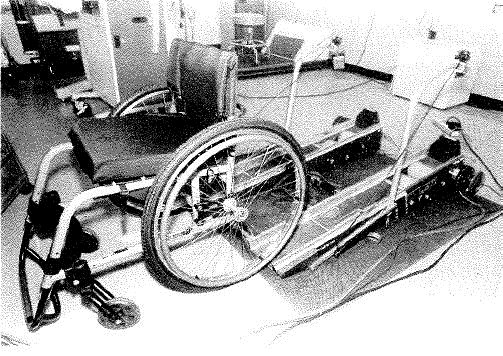
\includegraphics[scale = 25]{images/WAFT}
\caption{ Wheelchair Aerobic Fitness Trainer (WAFT) photograph \cite{langbein1993research}.}
\label{WAFT}
\end{figure}


Other roller ergometers have also been developed over the last four decades and particularly in the last fifteen years: Eagle Wheelchair Roller \cite{kerk1995effect}, Bromking Turbo Trainer \cite{goosey2001kinetic} \cite{goosey2001kinetic} \cite{ price1999thermoregulatory} or very recently the "Computer Monitored Wheelchair Dynamometer" \cite{cooper2003wheelchair}  \cite{digiovine2001dynamic}.  Other braking systems have been used, such as mechanical braking using a friction belt on a flywheel\\\cite{goosey1998relationship}  \cite{kulig2001effect} \cite{rodgers1994biomechanics}(Figure \ref{FRER}), an electric motor creating a frictional moment around the roller rotation axes \\\cite{coutts1987aerobic} \cite{kerk1995effect} \cite{patterson1997selected}     \\ \cite{vanlandewijck1999field} or an isokinetic apparatus  \cite{ruggles1994biomechanics}. To determine the speed, angular position sensors  \cite{brouha1967continuous}  \\ \cite{coutts1987aerobic}  \cite{coutts1990kinematics}  \cite{patterson1997selected} \\ \cite{rodgers1994biomechanics}, optical encoders   \cite{devillard1999wheelchair} \cite{devillard2001validation}   \\ \cite{langbein1993calibration}  \cite{langbein1994initial}  \cite{newsam1996temporal}  \\ \cite{theisen1996new}, tachometers  \cite{cooper1990exploratory}  \cite{kerk1995effect}   \cite{masse1992biomechanical} \\  \cite{vanlandewijck1999field} or speedometers   \cite{goosey1998relationship}  \cite{rodgers1994biomechanics} were used.

\begin{figure}[h]
\center
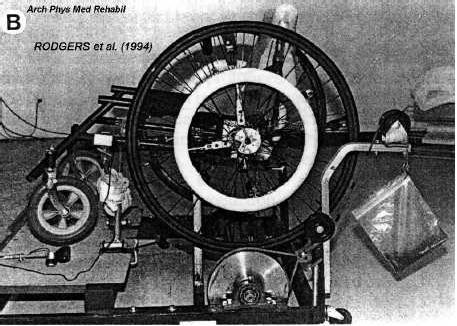
\includegraphics[scale = 25]{images/FRER}
\caption{Picture of a wheelchair on a roller ergometer with mechanical braking by friction belt on a flywheel. \cite{rodgers1994biomechanics}.}
\label{FRER}
\end{figure}

The main advantage of roller ergometers is that they allow subjects to be studied with their own MWC. Moreover, they occupy a little space in the laboratory and allow the MWC to be completely immobilized, thus ensuring the stability of the subject on the MWC and facilitating the measurement of  various physiological parameters. However, the various methods for estimating external  mechanical power used up to now still need to be refined to better evaluate this parameter. Furthermore, the comparison between the results of studies carried out with different roller ergometers and different mechanical models must be done with caution since the parameters neglected or taken into account are not all the same.

\subsection{Treadmill}
Like roller ergometers, the main advantage of treadmills is that they allow subjects to be studied with their own MWC. Since the four wheels of the MWC roll on the belt, the rolling friction forces are most certainly equivalent to those existing on the ground. Unlike roller ergometers, treadmills  allow to define a rolling speed of the belt and also a slope, that is, an inclination of the treadmill with respect to the horizontal. The main disadvantage of a treadmill comes from the steering problem related to the control of the trajectory: Indeed, a subject could drift and be ejected from the treadmill; to remedy this, railings have been installed on both sides using a surface strip that limits lateral movements \cite{claremont1985model}. However, it has still not been demonstrated that the propulsion technique used was identical on a treadmill and on the ground.

\begin{figure}[h]
\center
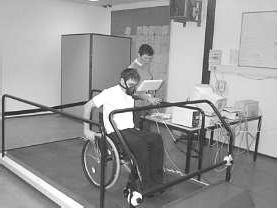
\includegraphics[scale = 40]{images/tapi_roulant}
\caption{ Exercise testing on a motor driven treadmill \cite{van2006manual}}
\label{tapi_roulant}
\end{figure}

\subsection{Wheelchair simulators}
To overcome the problems related to rolling resistance, some researchers chose to fix the rear wheels of the MWC without contact with the ground, on a rigid and fixed chassis on which the Subject could sit. The advantage of MWC simulators is that they can test different settings such as seat position or rear wheel camber angle, for example. The mechanical propulsion model is also simplified compared to roller ergometers and conveyor belts, which allows better quantification of work and external mechanical power.   However, the influence of the Subject's movements on the seat is not taken into account. This aspect is the major disadvantage of the simulators because neither the forces of resistance to the advance nor the kinematics of the MWC is modified according to the movements of the Subject on the seat.

\begin{figure}[h]
\center
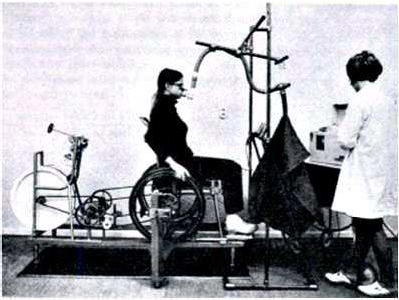
\includegraphics[scale = 30]{images/SFR}
\caption{Photograph of an experiment on a simulator connected to a flywheel (\cite{brattgaard1970energy})}
\label{SFR}
\end{figure}

\subsection{Wheelchair Field-Ergometer}
To analyse the efficiency of wheelchair propulsion, a Wireless Wheelchair Ergometer (WWE or FRET-1)  equipped with several sensors has been manufactured \cite{dabonneville2005self}. The sensors installed on the wheelchair measure the physical stresses applied to the MWC during actual use and record them.


The sensors are located on the right and left wheels of the MWC, on the footrest, on the seat and the backrest (Figure \ref{fret_legend}). These sensors measure the torques applied to each of the systems mentioned above.  The moment of a force concerning a given point is a vectorial physical quantity, which expresses (cf. explications Chap.\ref{application}) the ability of a force to turn a mechanical system around that point, often called a pivot. Other sensors installed on the FRET-2 are used to measure the kinematic parameters (speed, acceleration) of the movement of the MWC.


\begin{figure}[h]
\center
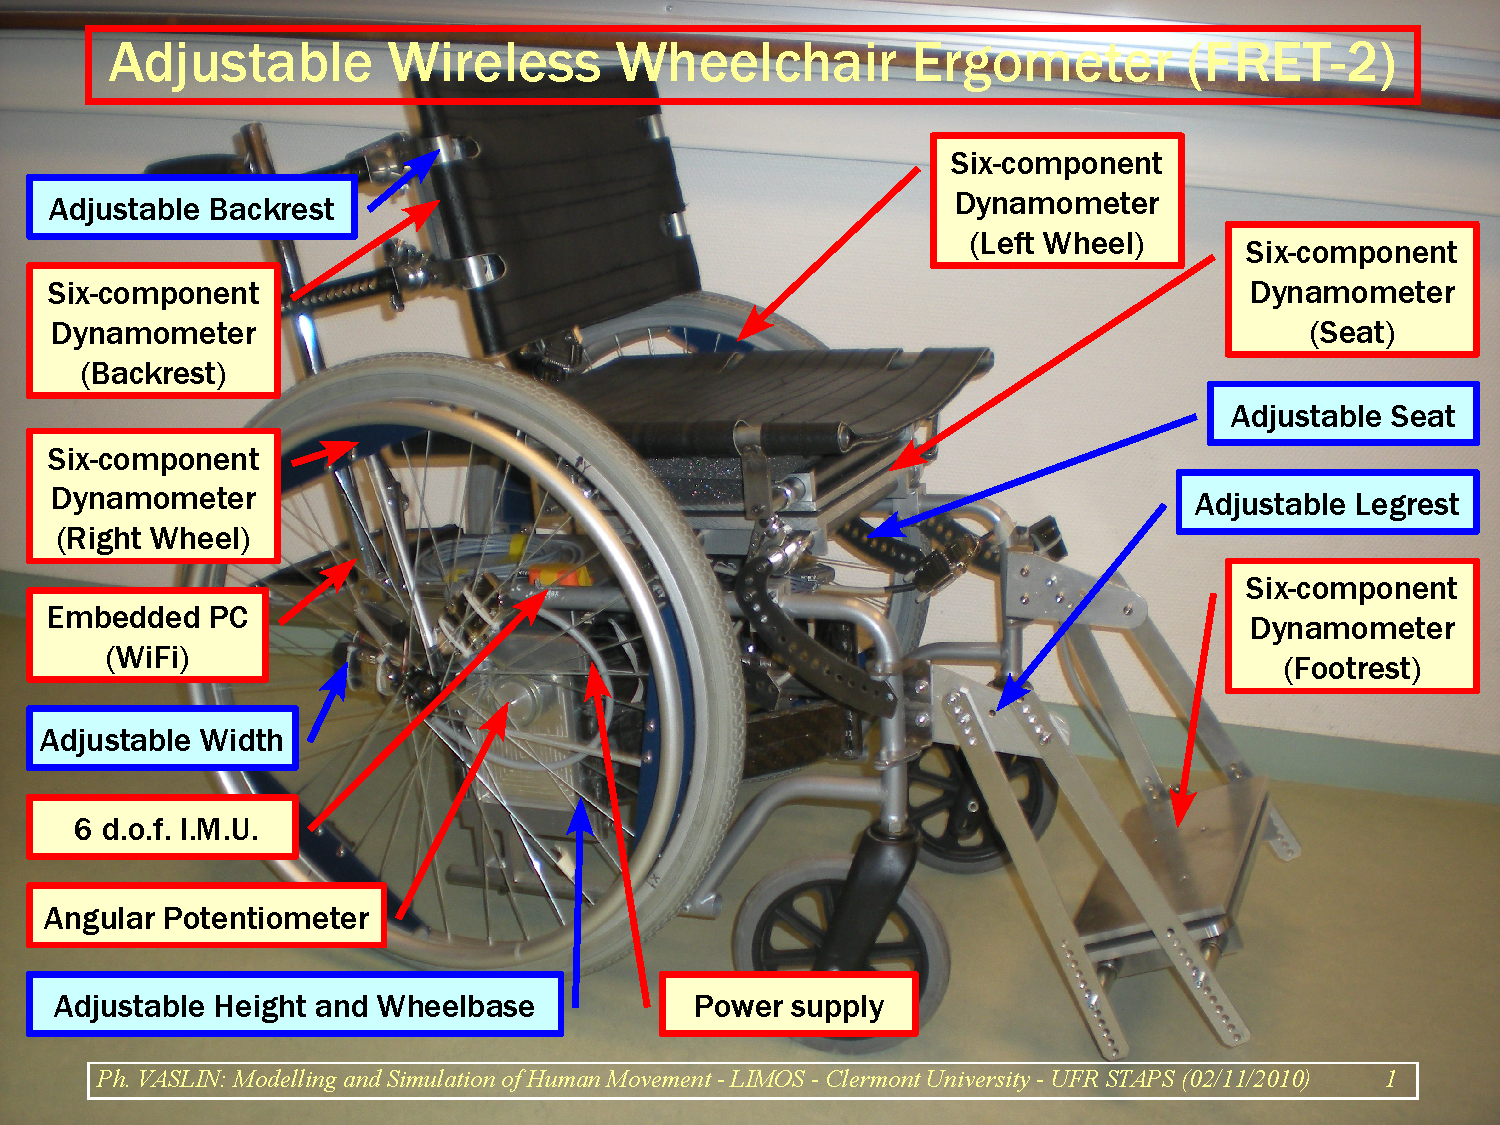
\includegraphics[scale = 0.4]{images/FRET-2_Legend_GB}
\caption{Captioned picture of the adjustable wireless wheelchair ergometer (FRET-2).}
\label{fret_legend}
\end{figure}


The measurements recorded by the sensors, which are the prupose of our analysis, consist of 44 attributes; of which 30 represent the dynamic parameters (Fx, Fy, Fz, Mx, My, Mz = 6 components x 5 dynamometers). The 14 other attributes represent the kinematic parameters of the MWC and its position relative to the Earth's magnetic North.

\section[Wheelchair time series]{Knowledge discovery on wheelchair time series}
After the construction ofthese measuring instruments (FRET-1 and FRET-2), they habe been used to measure the efforts made by MWC in actual conditions of wheelchair locomotion. Thus, several experiments have been conducted with several subjects,  where the efforts produced during actual wheelchair locomotion were measured with the FRET-2. The abundance of the recorded measurements highlighted the problem of the exploitation of these measures for knowledge extraction. Two main and complementary approaches can be used to analyze measurements from MWC locomotion. The first is to use mechanical models to calculate the physical parameters of motion and the second is to use data mining models to exploit measurements.  In this section, we present the contributions of these two approaches, which will allow us to position our work.



\paragraph{}Manual wheelchair locomotion causes significant mechanical stresses in the upper limbs. To remedy this problem, biomechanical studies have been conducted to identify and quantify traumatic factors such as:
\begin{itemize}
\item The doctoral thesis of Nicolas DE SAINT REMY (2005) \cite{Remy2005} who proposed a
mechanical model relating the forces applied to a MWC and its displacement ( Figure \ref{Wheelchair_model} ). This work particularly highlighted the fact that wheelchair acceleration is a function of subject's movements.

\begin{figure}[h]
\center
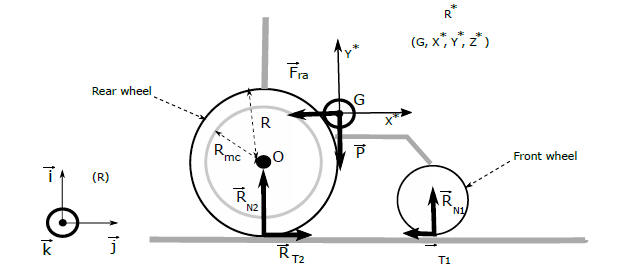
\includegraphics[scale = 0.6]{images/wheelchair_model2}
\caption{Balance of forces applied to a manual wheelchair during propulsion. For the clarity of the figure, the analysis of the movement of the {subject + MWC} system is reduced to that of the system's centre of gravity, G \cite{Remy2005}}
\label{Wheelchair_model}
\end{figure}

\item The doctoral thesis of Christophe SAURET (2010) \cite{Sauret2010} who proposed a method of calculating the mechanical power developed by manual wheelchair users to move. This model analyzes the kinetics of the {subject + MWC} system. For that purpose, the author developped a detailed kinematic model of the {subject + MWC} system (Figure \ref{Wheelchair_model2}) allowing to record their movements with a 3D motion analysis system during actual locomotion on the ground. 


\begin{figure}[h]
\center
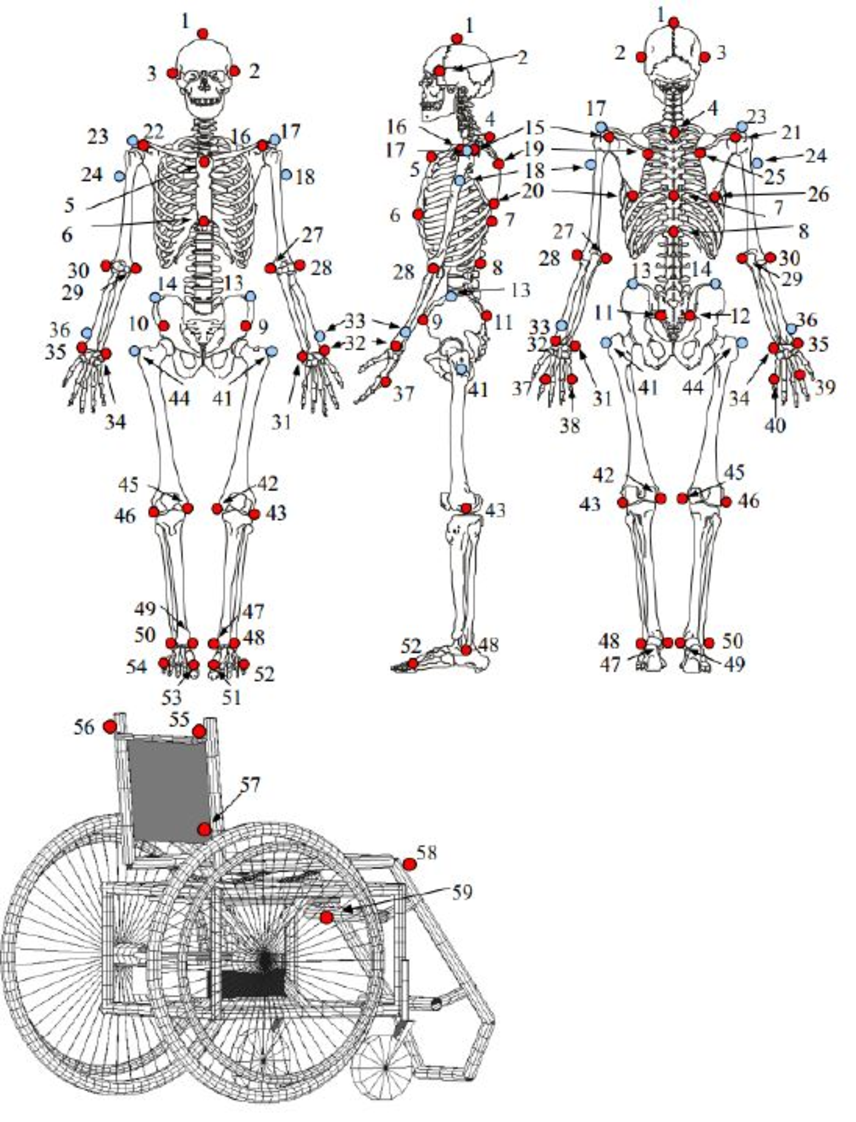
\includegraphics[scale = 0.5]{images/squelette}
\caption{Markers for kinematic analysis of manual wheelchair locomotion\cite{Sauret2010}}
\label{Wheelchair_model2}
\end{figure}

\end{itemize}


\paragraph{} More and more works in the literature suggest using the tools developed in data mining for a better understanding of human locomotion. For example, in \cite{van2017future}, the authors ask whether advances in data science and technology could provide a different and perhaps more objective view of the analysis of wheelchair users' motor abilities. On one hand, technical advances have made it possible to measure the efforts made by wheelchair users during their movement using sensors. On the other hand, datamining models have been proposed and allow to perform several task on the data (clustering, classification, …). 

In \cite{faria2012patient} the authors explained how they used robotics and data mining knowledge to build an Intelligent Manual Wheelchair. which can be controlled from multiple interfaces: joysticks, facial expressions, voice commands, head movements.  Since Intelligent Wheelchair users have various characteristics, a series of tests have been carried out to classify them and to define profiles that allow the MWC to be adjusted appropriately for each user.

In \cite{athanasiou2009bayesian} the authors presented a model based on Bayesian networks to improve the medical treatment of patients in wheelchairs with a spinal cord injury. Indeed, the treatment of these patients  is based on the level of spinal cord injury and symptoms. A lesion in the spine has three consequences: an inconsistency of the bowel, an inconsistency of the bladder, a loss of the skin sensitivity. The higher the lesion, the more widespread its effects on patients are. Thus a patient with a low lesion will affect the patient's legs  and a patient with a high lesion will see his four limbs affected. Because of this loss of sensitivity, symptoms observed in the patient are often incomplete, which introduces uncertainty into the diagnosis that is captured by Bayesian networks and conditional probabilities.





\section{Conclusion}



Throughout this chapter, we showed that there is a large number of MWC users in the world and that it is crucial to analyze this particular means of locomotion to improve the living conditions of people moving in a MWC. We have presented the main tools designed and manufactured for wheelchair locomotion analysis and some previous works that used data mining mechanics models to improve the study of wheelchair locomotion or  to help help physicians to diagnose the adverse for the adverse effects treatment of spinal cord injury causing paralysis and requiring the use of MWC. 


In the scientific literature,  mechanical or data mining models are used for manual wheelchair locomotion analysis.  In this thesis, however, we want to \textbf{design} data mining models that is able to take into account both the specificities of MWC locomotion data and their use to analyze wheelchair locomotion from a new point of view. In the next chapter, are presented the existing works in the literature of knowledge extraction on time-series, which will allow us to identify and then choose  useful approaches for the analysis of wheelchair locomotion.






\begin{table}[ht]
\centering
\begin{tabular}{|l|}

\hline
\rowcolor{LavenderBlush}
Key points\\
$\bullet$ The first section of the chapter \ref{locomotion_analysis} presents the three central research questions related \\ to the analysis of Manual Wheelchair locomotion \\ \; We explain why this thesis is focused on the study and improvement of motor skills of\\ Manual Wheelchair users. \\
\\
$\bullet$ The second section of the chapter \ref{locomotion_analysis} presents the measurement tools built to measure \\ the efforts  made by manual wheelchair users during their locomotion. Here we insist on \\ the Wheelchair Field  ergometer, which  produces the time series that we use throughout \\ our work for  the analysis of manual wheelchair locomotion. \\
\\
$\bullet$ The third section of the chapter \ref{locomotion_analysis} presents the mechanical models and data mining models \\ used in the literature for manual wheelchair locomotion analysis.\\

\hline
\end{tabular}
\end{table}





\chapter{Knowledge discovery on time series}
\label{kdd}

\section{Introduction}

Datasets can be grouped into four main categories regarding their temporality \cite{roddick2002survey}: 
\begin{itemize}
\item Static datasets: these are datasets with no temporal context. We have for example the radius of a wheel, the circumference of a circle, the gravity in a place.
\item Sequences datasets: they consist of   ordered sequences of events. This category includes an order but not time. As an example, we can cite a DNA sequence (GTTTTCCCAGTCACGAC).
\item Time-indexed datasets: they consist of a set of temporal data sequences ; for example a set of measures taken at a more or less regular time interval.
\item Full-time data: Each tuple has one or more time components; time series belongs to this latter category.
\end{itemize}

Time series have several characteristic properties: usually, they are noisy, uncertain and  
they often have high dimensionality and high auto-correlation. Each of those features can interfere with the mining of time series.  To remedy this, preprocessing technics have been proposed in the literature.
\section{Preprocessing of time series}


\subsection{Denoising time series}
Several filters have been proposed in the literature to remove noise contained in time series. In this section, the most  frequently used filters are presented.
\paragraph{Kernel smoothing:} this filter refers to a statistical technique for recovery of underlying structure in data sets. Its basic principle is to estimate a real-valued function as the weighted average of neighboring observed data. The weight is defined by a function named kernel, such that closer points to real values are given higher weights \cite{wand1994kernel}.

\paragraph{Polynomial Regression:} this filter consists in fitting a nonlinear relationship between the values of an independent variable x (predictor variable)  and the corresponding conditional mean of y (variable to explain), denoted E(y |x). This filter has been used to describe nonlinear phenomena. More formally, polynomial regression is defined as the problem of finding a polynomial:  $g(x)=\beta_{0}+\beta_{1}x+...+\beta_{m}x^{m}$ of a certain degree $m$ for wich $E(Y-g(x))^{2}$ is as small as possible \cite{kendall1961advanced}.

\paragraph{Wiener-Kolmogorov Filtering of Short Stationary Sequences:}  
The idea of this filter is to produce a statistical estimate of the actual signal from the noisy signal. Using the Wiener-Kolmogorov filter assumes the knowledge of stationary signal, noise spectra, and additive noise \cite{pollock2007wiener}.

\paragraph{Filtering in the Frequency Domain:}   The purpose of frequency-based filters is to remove the noise contained in a signal. To achieve this goal, the signal is initially broken down into a set of frequencies using a Fourier transform. This set of frequencies is called the signal spectrum. Depending on the application, it may be appropriate to suppress high or low frequencies, or both, to suppress signal noise. These filters are generally named low-pass, high-pass, bandpass, or notch filter. These filters can also be combined in many ways: in cascade, in parallel, etc \cite{buttkus2012spectral}.

\paragraph{Kalman Filter and the Smoothing Algorithm,} also known as linear quadratic estimation (LQE), is a Bayesian estimation technique used to track stochastic dynamic systems being observed with noisy sensors. The filter produces estimates of unknown variables that tend to be more accurate than those based on a single measurement alone, by estimating a joint probability distribution over the variables for each timeframe. The algorithm works in two phases: extrapolation (prediction) and update (correction). In the extrapolation step, the Kalman filter produces estimates of the current state variables, along with their uncertainties, based on the previous state variables and their uncertainties. Once the outcome of the next measurement is observed, these estimates are updated using a weighted average, with a higher weight being given to estimates with higher certainty. The algorithm is recursive. It can run in real time, using only the current input measurements and the previously calculated state and its uncertainty matrix \cite{matthies1989kalman}.



\subsection{Reducing uncertainty}
Another important step of preprocessing time series is to reduce the uncertainty that they contained. For this purpose some transformations have been introduced in literature.


\paragraph{Uncertain moving average:}   For uncertain time series, each value is associated with a standard deviation representing uncertainty. The uncertain moving average (UMA) filter is then defined as the weighted average of the consecutive data points of a time series over a given time interval. The weights at each timestamp $i$ are calculated from the inverse of the uncertainty. Thus, in the calculation of the mean, a weight $(w)$ inversely proportional to the uncertainty will be given to each data point in the time series. Uncertain moving average returns times series: $x^{UMA}=<x_{1}^{UMA},...,x_{m}^{UMA}>$ for which $x_{i}^{UMA}=\frac{1}{2w+1}\stackrel[k=i-w]{i+w}{\sum}\frac{x_{k}}{\sigma_{k}},\,1\leq i\leq m$ \cite{Orang2015}.

\paragraph{Z-normalization} is used with uncertain moving average to reduce the advert effect of uncertainty in time series. In general, z-normalization improves similarity search quality, because it makes similarity measures invariant to scaling and shifting. Given an uncertain time series: $X=<X_{1},...,X_{m}>,$ its normal form: $\hat{X}=<\hat{X}_{1},...,\hat{X}_{m}>$ is defined as follows: 

\[
\ensuremath{\hat{X}_{i}}=\frac{X_{i}-\overline{X}}{S_{X}},
\]
where $\overline{X}$ and $S_{X}$ denote the sample mean and standard deviation of expected values of X, respectively \cite{Orang2015}. That is,

\[
\overline{X}=\frac{1}{n}\stackrel[i=1]{n}{\sum}E(X_{i}),
\]

\[
S_{X}=\sqrt{\frac{1}{(n-1)}\stackrel[i=1]{n}{\sum}(E(X_{i})-\overline{X})^{2}}.
\]

\subsection{Dimensionality reduction}
Time complexity of a mining time series algorithm depends on the length of the time series. Reducing dimensionality of time series allows reducing their processing time. To achieve this goal, many representations have been proposed and can be grouped into three main categories: 

\paragraph{Non-data-adaptive:}Dimension reduction methods are called non-data-adaptive because they take parameters of which value does not vary according to the considered data set. One of the first work in this family was done by Agrawal \\ \cite{Agrawal1993} who used a Discrete Fourier Transform to compress time series. In the same family, we can also cite the following time series representations:  Discrete Wavelet Transform (DWT) \cite{chan1999efficient}, Piecewise Linear Approximation (PLA) \cite{eriksson2004piecewise}, Piecewise Aggregate Approximation (PAA) \cite{Keogh2001a}. 

\paragraph{Data adaptive:} This family of time series representation  consists of methods that take the properties of the dataset into account when choosing the method parameters. All non-data-adaptive representations can be transformed into data-adaptive representations by adding a parameter selection method to them. As examples of data-adaptive representations, there is Adaptive Piecewise Constant Approximation (APCA) \cite{keogh2001locally} and Singular Value Decomposition (SVD) \cite{de1994singular} and Symbolic Aggregate Approximation (SAX) \cite{lin2003symbolic}.

\paragraph{Model based:} The assumption here is that time series are described by an underlying model.  Dimensionality reduction is achieved by identifying the model parameters that generate the time series. Several approaches use temporal parametric models such as statistical modeling by feature extraction \cite{Esling2012}, Auto Regressive Moving Average (ARMA) models \cite{kalpakis2001distance}, Markov Chains (MCs) and Hidden Markov Models (HMM) \cite{panuccio2002hidden}.
\\

After cleaning the time series, we are now ready to extrat relevant information from them. Several data mining tasks can be performed with time series.

\section{Similarity Measures}

Before performing data mining tasks, it is essentia to be able to compare time series. Most often,  similarity functions compare time series as humans would do. Indeed, without much of stretch, human recognition understand and look at the likenesses between two time series based on their amplitude, scale, temporal warping, noise, and outliers. As indicated by \cite{fu2011review} \\ \cite{ralanamahatana2005mining}  \cite{Esling2012}, any similarity measure  for time series comparison ought to be reliable with human recognition and perception and have the following properties:


\begin{itemize}
\item It should perceive perceptually comparative datasets even if  they are not mathematically identical;
\item It should resemble human intuition;
\item It should be able to capture global and local similarities;
\item It should have a universal meaning that is not restricted to particular type of time series datasets and do not assume some constraints on time series data;
\item It should be robust to distortions and set of transformations. More specifically it should be robust to amplitude
shifting, uniform amplification, uniform time scaling, dynamic amplification, dynamic time scaling, adding noise and outliers transformations or any combination of these transformations.
\end{itemize}
The latter property is also known as invariance.

\subsection{Time-Series Invariances}
In this section, we review common time-series distortions and their invariances. More detailed information can be found in \cite{batista2014cid}. 

\paragraph{Scaling and translation invariances:} We should be able to perceive the similarity of sequences in spite of contrasts in amplitude (scaling) and offset (translation). For instance, these invariances may be helpful to analyze seasonal variations in currency values on foreign trade markets without being biased by inflation.


\paragraph{Shift invariance:}  We should be able to recognize two similar sequences even if they vary in phase (global alignment) or when there are regions of the sequences that are aligned and others are not (local alignment). For instance, heartbeats can be out of phase depending on when we start recording, and handwritings of the same sentence from various people will require alignment depending on the size of the letters and on the spaces between words (local alignment).


\paragraph{Uniform scaling invariance:} We should be able to compare two sequences even if they have different length. To do so, sequences that differ in length require either extending of the shorter sequence or, contracting of the longer sequence. For instance, this invariance is required for  heartbeats recorded at different sample frequencies  (e.g.: 10, 50 ou 100 Hz).  

\paragraph{Occlusion invariance:} We should be able to compare two time series even if some of their sub-sequences  are missing; we can also compare the sequences by ignoring the sub-sequences that do not match well.  For example, suppose an archaeologist who has just found a skull in a research site, and  would like to determine to which species this skull belongs. Let us also suppose that we have a database of time series corresponding to the skulls of living species. We could then compare the time series from the found skull to those stored in the database. This comparison should be possible even if the found skull is damaged. In other words, we should be able to make a comparison even if the time series extracted from the found skull has missing sub-sequences.

\paragraph{Complexity invariance:} We should be able to recognize time series with similar shape even if they have different complexity.  For example, the same audio signals that were recorded indoors and outdoors might be considered similar, although outdoor signals will surely be noisier than indoor ones. 


\\

Depending on the application domain, some or all the invariances can be required for the comparison of time series. The preprocessing step can handle some of those invariances; for instance, z-normalization of time series allows their comparison to be scaling invariant. However, all invariances cannot be handled by preprocessing step and should then considered by more sophisticated distances or dissimilarities functions. In the next section, we review the most common of such distance measures.





\subsection{Categories of time series similarity function}


Time series similarity measures can be generally divided into following four main categories:

\\

\textbf{Based similarity function} compares two time-series based on the sum of the distances in a Euclidian space between data points of both times series located at approximately the same timestamp. By doing so, the distance between two time series with similar shapes will be low. On the opposite, the distance between time-series that have a different shapes will be high. In this family, there are Lp norm \cite{yi2000fast} \cite{keogh2003need}, and Dynamic time warping distance \cite{ MyersRabinerRosenberg1980} for instance. However, those distances are sensitive to noise.

\\

\textbf{Edit Based distance} allows evaluating the dissimilarity between two character strings. These dissimilarity functions are able to handle noisy regions and outliers. The principle of these similarity functions is the following: Edit based distances count the minimum number of operation necessary to transform a character string to another. Different edit based dissimilarity functions use different operations to transform one string to another. A well known edit based distance is Levenshtein distance. That uses three operations: suppression, insertion and substitution of letters. Edit based distances in time series domain are based on the same principle. Time series data points can be skipped during the comparison (deletion) or one  data point can be compared to several data points of the other time series (insertion). Among the well-known  edit based distances in time series domain we can cited: Longest Common SubSequence (LCSS) \cite{das1997finding}, Edit Distance on Real sequence (EDR) \cite{chen2005robust} and Time Warp Edit Distance (TWED) \cite{marteau2009time} algorithms. LCSS distance uses a threshold parameter for point matching as well as a warping threshold for allowing gaps for matching two time series. EDR is a variant of the edit distance for real-valued series. Opposite to LCSS, EDR assigns penalties based on the length of existing gaps between two series. TWED is a dynamic programming algorithm that introduces a parameter to control the elasticity measure along the time axis. 

\paragraph{Feature Based distance:} this distance has been designed to ensure some invariances such as rotation invariance. Time series can be compared based on their properties rather than on their shape. So, Feature Based similarity measures compare two time series by computing a feature set for
each time series that reflects their properties\footnote{We will use this type of distance later when analyzing manual wheelchair locomotion (Chap. \ref{application}).}. For example, DFT and DWT coefficients can be used to compare the similarity between time series \cite{shatkay1996approximate}.


\paragraph{Structure Based similarity measures:}These measures are designed to compare time series on a global scale based on their structure. The general principle of those similarity functions is to compare time series based on a high-level representation that captures global properties of the time series, such as histogram, for instance  \cite{lin2009finding}.   



\section{Datamining task on time series}
\paragraph{Indexing time series: }
The problem of indexing or query by content can be defined as follows: given a query time series Q, and some similarity/dissimilarity measure D(Q,C), find the most similar time series in database DB. When querying time series by content, a challenge consists in finding as fast as possible a time series in the database that is similar to the query. To achieve this goal, some dimensionality reduction technics have been used:  for instance, in \cite{Agrawal1993}, time series have been transformed into a more compact representation using  DFT before their comparison. Many other dimensionality reduction techniques have been used for the same purpose, such as Discrete Wavelet Transform (DWT) and Discrete Cosine Transform (DCT) \cite{chan1999efficient}. Other representation approaches used for query by content are PLA, PAA, APCA \cite{keogh2001locally}, and SAX \cite{Lin2007}. These latter authors \cite{Lin2007}  have shown that SAX outperforms other representations for query by content applications.

\paragraph{Motif Discovery:}
Time series motifs are pairs of individual time series, or subsequences of a longer time series, which are very similar to each other and carry precise information about the underlying source of the time series. The idea for motif discovery in time series is inspired from DNA analysis. When they exist, motifs can be used to construct meaningful clusters when clustering time series, which is the case of unsupervised shapelet algorithm \cite{ulanova2015scalable}. Associating each class with a motif can speed-up the classification of time series; this idea is used by the shapelet transform algorithm\footnote{We will use this type of distance later when analyzing manual wheelchair locomotion (Chap. \ref{training_technic} ).} \cite{lines2012shapelet}.

\paragraph{Anomaly Detection:}
Anomaly detection refers to the problem of finding patterns in data that do not conform to the expected behavior. These nonconforming patterns are often referred to as anomalies, outliers, discordant observations, exceptions, aberrations, surprises, peculiarities, or contaminants in different application fields. Among these, anomalies and outliers are two terms  most commonly used in the context of anomaly detection; sometimes interchangeably. Anomaly detection finds extensive use in a wide variety of applications such as fraud detection for credit cards, insurance, or healthcare, intrusion detection for cyber-security, fault detection in safety-critical systems, and military surveillance of enemy activities \cite{chandola2009anomaly}.

\paragraph{Temporal Association Rule Discovery:}
In a transactional database, association rules allow searching for items that often appear together in the same transaction. For instance, in the database of a Shop, the discovered rules will indicate, which products are often bought together. The association rules do not give any information on the precedence of the occurrence of one event concerning the other. Hence the need to define temporal association rules,  which are particularly appropriate as candidates for causal rules' analysis in temporally adorned medical data, such as in the histories of patients' medical visits. Patients are associated with both static properties, such as gender, and temporal properties, such as age or current medical treatments, any or all of which may be taken into account during mining \cite{Vasimalla2017}.

\paragraph{Summarization (Visualization):}
The problem of time series visualization or summarization can be defined as follows: given a time series $Q$ containing $n$ data points where, $n$ is an extremely large number, create a (possibly graphics) approximation of $Q$ which retains its essential features but fits on a single page, computer screen, executive summary. Summarization can be viewed as a higher level clustering of time series  where clusters are associated with text or graphical descriptions. Some famous approaches of time series summarization  are:
\begin{itemize}

\item    \textbf{Time searcher}: it is a query by content summarization tool. Here, a user specifies a set of constraints (intervals) graphically to which time series data points should belong. Those constraints are called time series boxes \\ \cite{hochheiser2003interactive}.
\item    \textbf{Calendar based visualization} of univariate time series data: its goal is to simultaneously identify patterns and trends on multiple time scales (days, weeks, seasons). To do so, Calendar based visualization first clustered similar daily data patterns and visualized the average patterns as graphs and the corresponding days on a calendar \cite{van1999cluster}. 
\item    The \textbf{spiral visualization} is appropriated with large data sets and supports much better than line graphs the identification of periodic structures in the data. Spiral visualization supports both the visualization of nominal and quantitative data based. The extension of the spiral visualization to 3D gives access to concepts for zooming and focusing and linking in the data set \cite{weber2001visualizing}. 
\item    \textbf{GrammarViz} is a visualization tool that allows efficient discovery of frequent and rare patterns  of variable length in time series. It is based on the symbolic representation of time series sax and context-free grammar \cite{senin2014grammarviz}.
\end{itemize} 

\paragraph{Prediction} or time series forecasting is one of the most useful data mining tasks on time series: for example, time series forecasting is used to predict the weather, the cost of an action in the stock exchange market, or early identified epidemiological risks and raised up alarms. A time series forecasting method is based on a mathematical model that capture the main characteristics of the time series like seasonality, periodicity, trend, and that can be used to guess unknown (or future) values of the time series. Many other algorithms used for time series forecasting are based on Auto-Regressive (AR) models. More sophisticated approaches are also used such as neural networks and cluster function approximation \cite{mahalakshmi2016survey}.
\paragraph{Classification:}
Classified time series consists of assigning an unlabelled time series to one, two or more classes. Many classification algorithms for time series have been proposed in the literature and can be gathered into four main groups
\begin{itemize}
\item \textbf{Dictionary classifiers}: generally, these classifiers first transform time series into characters strings that can be decomposed into a set of word or bag of words, a word being simply a subsequence of the characters string. Each time series is then described by the occurrence frequency of each word in it. The set of time series represented in the space of words is called a dictionary; The classification of time series is then based on the presence or absence of words in this dictionnary. Several algorithms of the literature are based on this principle, such as Bag of Patterns \cite{lin2012rotation},  SAX and Vector Space Model \cite{senin2013sax}, Bag of SFA Symbols(BOSS) \cite{schafer2015boss} and DTW Features\cite{kate2016using}.

\item \textbf{Classifier-based on the alignment of whole time series}: those classifiers are based on distance functions that operate over the entire length of the time series. The difference between the classifiers of this family is based in part on the characteristics of the distance functions used. These distance functions can be based on the shape of the time series (Derivative Dynamic Time Warping  \cite{keogh2001derivative}, Weighted Dynamic Time Warping  \cite{jeong2011weighted}, Complexity-Invariant Distance  \cite{batista2011complexity}), on their properties, on their structures or on their symbolic representation (Time Warp Edit Distance \cite{marteau2008time}, Move Split Merge \cite{stefan2013move}).

\item \textbf{Shapelets Classifiers:}  Unlike classifiers based on the comparison of the time series over their entire length, shapelets classifiers look for characteristic sub-sequences in time series called shapelet whose presence or absence indicates whether or not a time series belongs to a class. We have for example: Shapelet Transform \cite{lines2012shapelet}, Learned Shapelets \cite{grabocka2014learning}, Fast Shapelet Tree \cite{rakthanmanon2013fast}

\item \textbf{Intervals Classifiers:} The idea here is to find localized discriminatory features on time series based on some statistical properties calculated over intervals of variable length. A time series of length $m$ will have $ m(m-1)/2$ possible contiguous intervals. An interval associated with some statistical properties and a condition is a literal, which gives some information about what happened in an interval: for instance, is the mean of a sequence of data points greater or less than a define threshold? The classifier tries to find a relationship between what happened in an interval and  time series classes. Many classifiers are based on this principle, such as: Time Series Bag of Features  \cite{baydogan2013bag}, Time Series Forest  \cite{deng2013time}, Learned Pattern Similarity  \cite{baydogan2016time}.
\end{itemize}


\paragraph{Clustering:}
The clustering of time series consists of grouping them to build very homogeneous and well-separated groups under some similarity/dissimilarity measure D(Q, C) \cite{rani2012recent}. "Homogeneous" means that the intra-group variance is small and "Well separated" means that the inter-groups variance is high. There are many ways to categorize time series clustering algorithms depending on the \textbf{distance function} used, the \textbf{data transformation} or  the \textbf{clustering strategy}. 


When considering \textbf{distance function}, we have two categories of time series clustering algorithms: those that operate on the whole time series and those that operates on a sub-sequences of time series.


 When considering \textbf{data transformation}, we can  gather time series clustering algorithms into three groups:  raw data, feature-based and model-based clustering. 


When considering \textbf{clustering strategy}, we have five categories of clustering algorithms: 

\begin{itemize}
\item   \textbf{Distance-based} clustering, which is divided in two sub-categories:
	\begin{itemize}
	\item \textbf{Partitioning clustering algorithms}  partition the data in        	high dimensional space into multiple clusters. We have for example kMeans like 		algorithms (kMeans, kMedians, kMedoids, XMeans, KMeans++)
	\item \textbf{Hierarchical clustering algorithms} are grouped into two 				subcategories: \textbf{Agglomerative clustering algorithms} first consider each 		object of the dataset as a cluster and then try to merge clusters until  obtainning 		one cluster: it is a bottom-up merging strategy. \textbf{Divisive clustering 			algorithms} first considers that all the data points are in the same cluster 		and then try to split this cluster to obtain more homogenous ones: it is the top-down merging strategy.
	\end{itemize}
   
\item \textbf{Density-Based clustering and grid-based clustering algorithm}:
 
\begin{itemize}
	\item The principle of \textbf{density-based clustering} is the following:   given a time 		series that will be considered as the center of the cluster,  all the time series of the database that have a distance less or 		equal to a defined threshold to the center of the cluster are gathered. Thus, the 			algorithm splits the space into more or less dense regions; then small dense  			regions can be merged into more significant regions. This algorithm allows to identify  		clusters of arbitrary shapes  \cite{kriegel2011density}.
	\item \textbf{Grid-based clustering} divides the data space into a grid-like 				structure, which allows determining the characteristics of the data \cite{amini2011study}.
\end{itemize}


\item \textbf{Probabilistic and generative models} can be modelled  with a generative process assuming the data follow a particular distribution like a mixture of Gaussian. Then the model parameters are estimated using the expectation-maximization algorithm (EM), that consider the parameters that maximize the likelihood of the model to the data. On this basis we may estimate the generative probabilities that will be used to construct the generative model \cite{merugu2003privacy}.


\item  \textbf{High-dimensional clustering algorithms}: time series may be set in a high dimensional feature space. To cluster them, many methods have been proposed:

\begin{itemize}
	\item  \textbf{Subspace clustering}: Subspace clustering looks for a cluster in 	different subspaces of a dataset.  A subspace is a subset of the $d$ dimensions 		of a given dataset; all the dimensions of high dimensional data are not useful. 	Subspace clustering algorithm identifies relevant dimensions allowing them to 		find clusters. There are two main subspace clustering branches based on their 		search strategy. Top-down algorithms find an initial clustering in the full set 		of dimensions and evaluate the subspaces of each cluster, iteratively improving 	the results. Bottom-up approaches find dense regions in low dimensional spaces 		and combine them to form clusters \cite{parsons2004subspace}.
	\item \textbf{Dimensionality reduction}: many dimensionality reduction 				techniques have been proposed for clustering purpose. A well-known one is co-clustering, which consists of simultaneously clustering  columns (or dimensions) 	and	rows (data points) of a matrix \cite{dhillon2003information}.
	\item \textbf{Probabilistic latent semantic indexing (PLSI)} and \textbf{laten 		dirichlet allocation (LDA)}  are typical clustering techniques for text data. Indeed, text can be clustered in multiple topics and  each topic can be associated with a 		set of words (or dimension) or a set of rows (documents) can be simultaneously associated 			\cite{hofmann2017probabilistic}.
	\item \textbf{Nonnegative matrix factorization} is a kind of co-clustering 			algorithm. It proceeds as follows: a nonnegative matrix X \in $\mathbb{R}^{M			\times N}$ can be 			factorised into two lower rank matrices U \in $			\mathbb{R}^{M\times L}$ and V \in $\mathbb{R}^{L\times N}$ with $L < M$ and $L 		< N$.  The idea here is to identify clusters using the matrix $U$ which has a lower 	dimension than $X$  						\cite{wang2013nonnegative}.
	\item \textbf{Spectral clustering}: the principle is to cluster time series or 		data objects based on the spectrum of their similarity matrix. The spectrum 			being used here for dimensionality reduction  \cite{filippone2008survey}.
	
\end{itemize}
 

\end{itemize}
In the context of this thesis, the analysis of manual wheelchair locomotion implies to grouping  manual wheelchair users with similar motor abilities, based on measurements made during their locomotion in actual conditions: this approach is  equivalent to time series clustering. Several clustering algorithms proposed in the literature are harmonious compositions, consisting of a representation of time series, an adequate distance function and an appropriate clustering strategy as illustrated in the Tables \ref{tab:1}, \ref{tab:2} and \ref{tab:3}. Detailed informations is presented in \cite{rani2012recent}. 

 
 
\begin{landscape}
% Please add the following required packages to your document preamble:
% \usepackage[normalem]{ulem}
% \useunder{\uline}{\ul}{}
\begin{table}[ht]
\centering
\small
\caption{Temporal-Proximity-Based Clustering Approach}
\label{tab:1}
\begin{tabular}{|l|l|l|l|}
\hline
\multicolumn{1}{|c|}{\textbf{Paper}}                           & \multicolumn{1}{c|}{\textbf{Distance Measure}}                                                                                               & \multicolumn{1}{c|}{\textbf{Algorithm}}                                                  & \multicolumn{1}{c|}{\textbf{Application}}                                                       \\ \hline
M. Kumar                                                       & \begin{tabular}[c]{@{}l@{}}Based      on      the      assumed  independent   \\   Gaussian models   of\\   data errors\end{tabular} & Agglomerative Hierarchical                                                               & Seasonality pattern in retails                                                                  \\ \hline
T.-W. Liao                                                     & \begin{tabular}[c]{@{}l@{}}Euclidean      and    symmetric\\   version    of    Kullback–Liebler\\   distance\end{tabular}             & \begin{tabular}[c]{@{}l@{}}K-Means\\   and Fuzzy C-Means\end{tabular}                    & Battle simulations                                                                              \\ \hline
T.-W. Liao                                                     & Dynamic Time Warping                                                                                                                         & \begin{tabular}[c]{@{}l@{}}K-Medoids    Based     Genetic\\   Clustering\end{tabular} & Battle simulations                                                                              \\ \hline
C.S. Möller-Levet                                              & \begin{tabular}[c]{@{}l@{}}Short     time     series     (STS)   distance\end{tabular}                                                     & Modified Fuzzy C-Means                                                                   & DNA microarray                                                                                  \\ \hline
Shumway                                                        & \begin{tabular}[c]{@{}l@{}}Kullback–Leibler\\   discrimination         information measure\end{tabular}                                      & Agglomerative Hierarchical                                                               & \begin{tabular}[c]{@{}l@{}}Earthquakes     and     mining  explosions\end{tabular}   \\ \hline
Vit Niennattrakul                                              & Dynamic Time Warping                                                                                                                         & K-Means, K-Medoids                                                                       & \begin{tabular}[c]{@{}l@{}}Multimedia time\\   series\end{tabular}                              \\ \hline
\begin{tabular}[c]{@{}l@{}}Pooya Sobhe\\   Bidari\end{tabular} & Pearson Correlation                                                                                                                          & K-Means, Fuzzy C-Means                                                                   & Pattern extraction in genes                                                                     \\ \hline
Hardy Kremer                                                   & Dynamic Time Warping                                                                                                                         & \begin{tabular}[c]{@{}l@{}}Density   Based \\    Subsequence\\   Clustering\end{tabular} & \begin{tabular}[c]{@{}l@{}}Detecting climate\\   change\end{tabular}                            \\ \hline
Jian Yin                                                       & Grey Relation                                                                                                                                & Hierarchical Clustering                                                                  & \begin{tabular}[c]{@{}l@{}}Change  trend  of\\    traffic  flow  data\end{tabular}       \\ \hline
S. Chandrakala                                                 & Euclidean                                                                                                                                    & Kernal DBScan                                                                            & \begin{tabular}[c]{@{}l@{}}Multivariate       time     \\    series\\   clustering\end{tabular} \\ \hline
Aurangzeb Khan                                                 & Euclidean                                                                                                                                    & \begin{tabular}[c]{@{}l@{}}K-Mean+ MFP(Most Frequent\\   Pattern)\end{tabular}           & Stock and inventory data                                                                        \\ \hline
Mengfan Zhang                                                  & \begin{tabular}[c]{@{}l@{}}CVT(Computational          Verb\\   Theory)\end{tabular}                                                          & K-Means                                                                                  & Stock market data                                                                               \\ \hline
S.R.Nanda                                                      & Euclidean                                                                                                                                    & K-Means                                                                                  & Portfolio management                                                                            \\ \hline
Jianfei Wu                                                     & N/A                                                                                                                                          & K-Means                                                                                  & Stock data                                                                                      \\ \hline
\end{tabular}
\end{table}
\end{landscape}



\begin{landscape}
\begin{table}[ht]
\centering
\small
\caption{Representation-Based Clustering Approach Paper}
\label{tab:2}
\begin{tabular}{|l|l|l|l|l|}
\hline
\multicolumn{1}{|c|}{\textbf{Paper}} & \multicolumn{1}{c|}{\textbf{Features}}                                     & \multicolumn{1}{c|}{\textbf{\begin{tabular}[c]{@{}c@{}}Distance\\   Measure\end{tabular}}}                                    & \multicolumn{1}{c|}{\textbf{Clustering Algorithm}}                                 & \multicolumn{1}{c|}{\textbf{Application}}                                              \\ \hline
T.-C. Fu                             & \begin{tabular}[c]{@{}l@{}}Perceptually important\\   points\end{tabular}  & \begin{tabular}[c]{@{}l@{}}Sum of the mean\\   squared distance along the\\   vertical and horizontal\\   scales\end{tabular} & Modified SOM                                                                       & Hong Kong stock market                                                                 \\ \hline
M. Vlachos                           & \begin{tabular}[c]{@{}l@{}}Haar wavelet\\   transform\end{tabular}         & Euclidean                                                                                                                     & Modified k-means                                                                   & Non-specific                                                                           \\ \hline
Huiting Liu                          & \begin{tabular}[c]{@{}l@{}}Empirical mode\\   decomposition\end{tabular}   & Euclidean                                                                                                                     & \begin{tabular}[c]{@{}l@{}}Forward propagation\\   learning algorithm\end{tabular} & Non-specific                                                                           \\ \hline
Chonghui GUO                         & \begin{tabular}[c]{@{}l@{}}Independent component\\   analysis\end{tabular} & Euclidean                                                                                                                     & Modified k-means                                                                   & \begin{tabular}[c]{@{}l@{}}Real world stock time-\\   series\end{tabular}              \\ \hline
Jian Xin Wu                          & \begin{tabular}[c]{@{}l@{}}Independent component\\   analysis\end{tabular} & N/A                                                                                                                           & \begin{tabular}[c]{@{}l@{}}support vector\\   regression\end{tabular}              & Financial time-series                                                                  \\ \hline
Geert Verdoolaege                    & Wavelet transform                                                          & \begin{tabular}[c]{@{}l@{}}Kullback- Liebler\\   divergence\end{tabular}                                                      & k-means                                                                            & \begin{tabular}[c]{@{}l@{}}Detection of activated\\   voxels in FMRI data\end{tabular} \\ \hline
Liu Suyi                             & Hough transform                                                            & N/A                                                                                                                           & Mean shift algorithm                                                               & \begin{tabular}[c]{@{}l@{}}Feature recognition of\\   underwater images\end{tabular}   \\ \hline
Dong Jixue                           & Wavelet transform                                                          & N/A                                                                                                                           & \begin{tabular}[c]{@{}l@{}}Grid-based partitioning\\   method\end{tabular}         & Financial time-series                                                                  \\ \hline
\end{tabular}
\end{table}
\end{landscape}


\begin{landscape}
\begin{table}[ht]
\centering
\small
\caption{Model-Based Clustering Approach}
\label{tab:3}
\begin{tabular}{|l|l|l|l|l|}
\hline
\multicolumn{1}{|c|}{\textbf{Paper}} & \multicolumn{1}{c|}{\textbf{Model}}                                                     & \multicolumn{1}{c|}{\textbf{Distance measure}}                      & \multicolumn{1}{c|}{\textbf{\begin{tabular}[c]{@{}c@{}}Clustering\\   algorithm\end{tabular}}} & \multicolumn{1}{c|}{\textbf{Application}}                                              \\ \hline
Baragona                             & ARMA                                                                                    & \begin{tabular}[c]{@{}l@{}}Cross-correlation\\   based\end{tabular} & \begin{tabular}[c]{@{}l@{}}Tabu    search,  \\    GA\\   and\end{tabular}                      & Non-specific                                                                           \\ \hline
K. Kalpakis                          & AR                                                                                      & Euclidean                                                           & Partitioning   around medoids                                                                  & Public data                                                                            \\ \hline
Xiong and Yeung                      & ARMA mixture                                                                            & Log-liklihood                                                       & EM learning                                                                                    & Public data                                                                            \\ \hline
L. Wang                              & Discrete HMM                                                                            & Log-liklihood                                                       & EM learning                                                                                    & \begin{tabular}[c]{@{}l@{}}Tool        \\    condition\\   monitoring\end{tabular}     \\ \hline
Xin Huang                            & \begin{tabular}[c]{@{}l@{}}Fuzzy  set\\    and\\    R/S\\   analysis model\end{tabular} & N/A                                                                 & \begin{tabular}[c]{@{}l@{}}Fuzzy     \\    clustering iteration method\end{tabular}            & \begin{tabular}[c]{@{}l@{}}Predicting\\   agriculture drought\end{tabular}             \\ \hline
Shan Gao                             & ARMA-ARCH                                                                               & N/A                                                                 & N/A                                                                                            & \begin{tabular}[c]{@{}l@{}}To analyze the\\   effects of wind data series\end{tabular} \\ \hline
\end{tabular}
\end{table}
\end{landscape}


\section{Conclusion}
Time series are ubiquitous in science and are more and more used in the analysis of human locomotion. This chapter presents a general framework for extracting knowledge from time series, starting by time series pre-processing, which allows reducing the advert effects of noise, uncertainty, and dimensionality. Then, we present strategies that are used to compare time series, and we finally present data mining tasks on time series. This chapter presents what has been already done in the literature and raises the question of extracting relevant information from time series coming from wheelchair locomotion. The following chapters present some new strategies that we introduce and that are adapted to characteristics of time series issued from manual wheelchair locomotion.

\begin{table}[ht]
\centering
\begin{tabular}{|l|}

\hline
\rowcolor{LavenderBlush}
Key points\\
We highlight the different models of data mining present in the literature that could\\ be useful to our work, particularly for  \\
\\
$\bullet$ Pre-processing of time series (noise reduction, dimensionality reduction) \\
$\bullet$ Comparison of time series.\\ 
$\bullet$ The different data mining tasks performed on time series.\\
\hline
\end{tabular}
\end{table}
\part{Contributions}
\chapter[Preprocessing of time series]{Compression for a better classification with Dynamic Time Warping}

\begin{abstract}
 Dynamic Time Warping (DTW) is a time series alignment algorithm that is often used because it
 considers that it exits small distortions between time series during their alignment.  However, DTW
 sometimes produces pathological alignments that occur when, during the comparison of two time series
 X and Y, one data point of the time series X is compared to a large subsequence of data points of Y.
 In this paper, we demonstrate that to compress time series using Piecewise Aggregate Approximation
 (PAA) is a simple strategy that greatly increases the quality of the alignment with DTW this is
 particularly true for synthetic data sets.      
 \end{abstract}

\section{Introduction}

Time series databases are often large and several transformations have been
introduced in order to represent them in a more compact way. One of these transformations is
Piecewise Aggregate Approximation (PAA) \cite{keogh2001dimensionality}, which consists in dividing a
time series into several segments of fixed length and replacing the data points of each segment with
their averages. Due to its simplicity and low computational time, PAA has been widely used as a
basic primitive by other temporal data mining algorithms such as \cite{lin2003symbolic,
sun2014improvement, lkhagva2006extended}, in order  
\begin{itemize}
  \item To construct symbolic representations of time
series; \cite{camerra2010isax, ulanova2015scalable}.
  \item To construct an index for time series; \cite{zhao2016shapedtw,
keogh2000scaling, Kate2016}. Indeed, PAA allows queries which are shorter than length for which the
index was built, this very desirable feature is impossible in Discrete Fourier Transform, Singular
Value Decomposition and Discrete Wavelet Transform.
\item To classify time series.
\end{itemize}


\subsection{Why the use of PAA can improve alignment with Dynamic Time Warping}

An important task is time series comparison  that
can be done in two main ways.
Either the comparison method  considers that there is no time distortion as in Euclidian distance
(ED), or it considers that  some small time distortions  exist between time axis of time series as
in Dynamic Time Warping alignment algorithm (DTW)
\cite{ZhangTangDuan2015}. Since time distortion often exists between time series, DTW often has
better results than the ED \cite{UCRArchive}. An exhaustive comparison of time series algorithms
\cite{Bagnall} shows that DTW is among the efficient techniques to be used. However, DTW has two major
drawbacks:
 the comparison of two time series under DTW is time-consuming
\cite{Rakthanmanon2012} and  DTW
sometimes produces pathological alignments \cite{KeoghPazzani2001}. A
pathological alignment occurs when, during the comparison of two time  series $X$
and $Y$, one datapoint of the time series $X$ is compared to a large subsequence
of datapoints of $Y$.  A pathological alignment causes a wrong comparison.


 Three categories of methods are used to avoid pathological alignments with DTW:

\begin{itemize}
  \item The first one adds constraints to DTW \cite{RatanamahatanaKeogh2004, YuYuHuLiuWu2011, candan2012sdtw, SakoeChiba1978, jeong2011weighted}.
  The main idea here is to limit the length of the subsequence of a time series
  that can be compared to a single datapoint of another time series.
  
  \item The second one suggests skipping datapoints that
  produce pathological alignment during the comparison of two time series \cite{longin2005elastic, itakura1975minimum, MyersRabinerRosenberg1980}.
  \item The third one proposes to replace the datapoints of time
  series with a high-level abstraction that captures the local behavior of those
  time series. A high-level abstraction can be a histogram of values that
  captures the repartition of time series datapoints in space \cite{ZhangTangDuan2015} or a 
  feature that captures the local  properties of time series, such as the trend with Derivative DTW
  (DDTW) \cite{KeoghPazzani2001}.
\end{itemize}
Another simple but yet interesting way to capture local properties of time series is to consider
mean of segments of the time series as PAA does. Indeed, the use of the mean reduces the harmful
effects of singularities contained in the data and thus allows to avoid the pathological
alignments.  However, one major challenge with PAA is the choice of the number of segments to
consider especially with long time series.


\subsection{The problem of choosing a suitable segment number for PAA}

If the number of segments considered with PAA is too small, the resulted
representation  is compact, but it contains less information. On the other side, if the number of
segments is too large, the obtained representation  is less compact and more prone to the noise
contained in the original time series (Fig. \ref{relation_nb_acc}). Our idea is that a number of
segments for PAA will be considered as good if it allows obtaining a compact representation of the
time series, and also if it preserves the quality of the alignment of time series. So when
considering classification task, one of the best classification algorithm to use for
evaluating the quality of time series alignment is one nearest neighbor (1NN).   
Indeed, its classification error directly depends on time series alignment, since 1NN has no other
parameters \cite{wang2013experimental}.


\begin{figure}[h]
\center
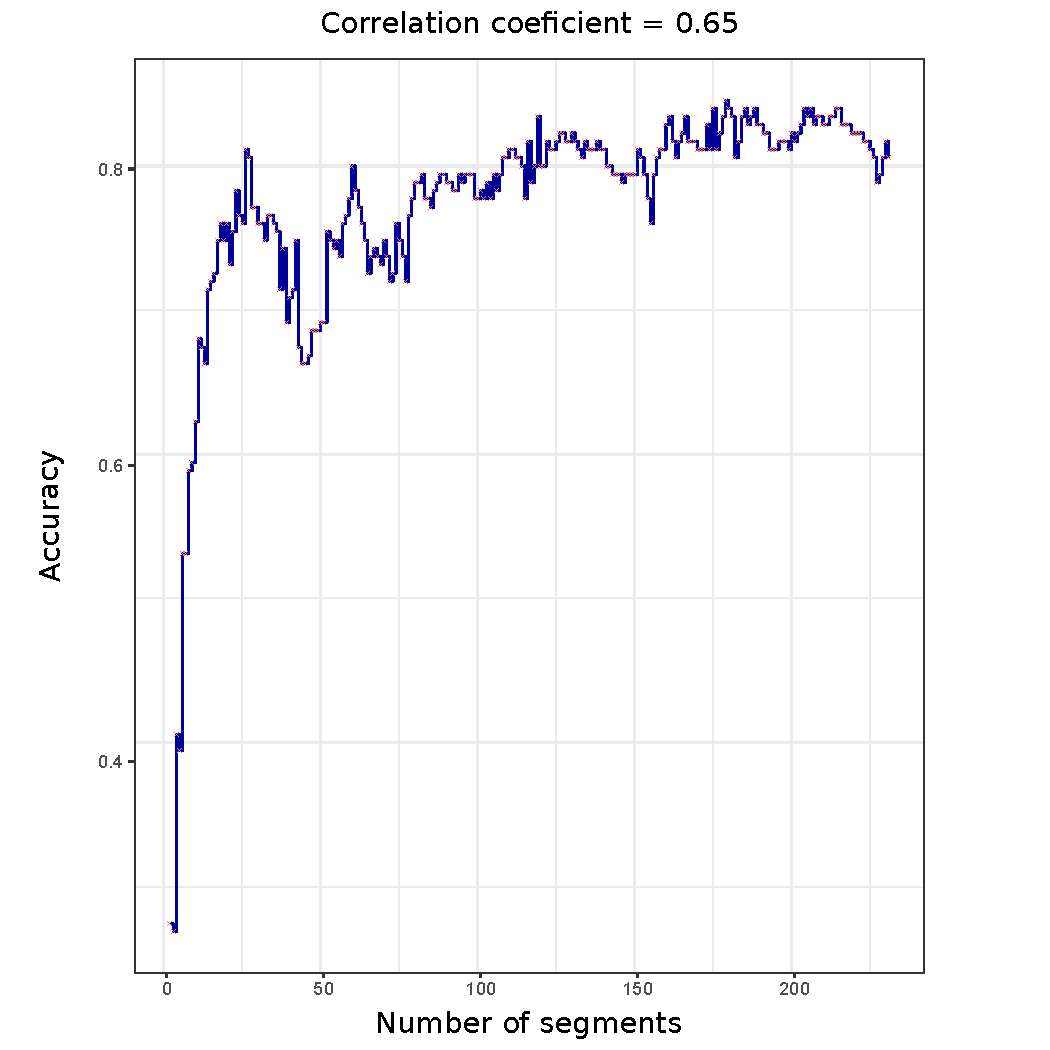
\includegraphics[scale = 0.4]{images/effets_de_n_sur_accuracy}
\caption{Relation between Accuracy and the number of segment on FISH dataset. The accuracy is computed from the algorithm one nearest neighbor associated with PDTW. When the number of segments
considered is very small, there is a loss of information and the accuracy is reduced. However, considering all the points in the time series, we also do not obtain maximum accuracy due to the presence of noise or singularities \cite{KeoghPazzani2001}  in the data. }
\label{relation_nb_acc}
\end{figure}

\subsection{Summary of Contributions}

In this paper, 
\begin{itemize}
\item We define the problem of preprocessing time series with PAA for a better classification with
DTW.
\item We propose a parameter free heuristic for aligning piecewise aggregate time series with DTW, which approximates the optimal value of the number of segments to be considered with PAA. 
\item  We make our source code and all our results available to allow the reproducibility of
our experiments.
work.
\end{itemize}

The rest of the paper is organized as follow: In Section
\ref{sec:1} we recall the definitions and background. Section \ref{sec:2} explains our approach.
Section \ref{sec:3} presents experimental results and comparisons to others methods. Section
\ref{sec:4} offers conclusions and venues for future work.   


\section{Background and related work}
\label{sec:1}
Let's recall some definitions.

\begin{definition}:  A \textbf{time series}
$X=x_{1},\cdots,x_{n}$ is a sequence of numerical values representing the evolution of a specific quantity over time. $x_{n}$ is the most recent value.
\end{definition}

\begin{definition}:
A segment  $X_{i}$ of length  $l$ of the time series $X$ of length $n$
$(l<n)$ is a sequence constituted by $l$ \hyphenation{conse-cutive} variables of $X$ starting at the position $i$ and ending at the position $i+l-1$.
We have: $X_{i}=x_{i},x_{i+1},...,x_{i+l-1}$
\end{definition}

\begin{definition}:
The arithmetic average of the data points of a segment  $X_{i}$ of length
$l$ is noted $\bar{X}_{i}$ and is defined by:
\begin{eqnarray}
\bar{X}_{i}=\frac{1}{l}\sum_{j=0}^{l-1}x_{i+j}
\end{eqnarray}

\end{definition}

\begin{definition}:
Let $T$ be the set of time series. The Piecewise Aggregate Approximation (PAA) is defined as follows:

\begin{eqnarray}
\begin{array}{ccc}
 PAA: T\times\mathbb{N^{*}}\rightarrow T\\
\\
(X,N)\mapsto PAA(X,N) & = &
 \begin{cases}
 \begin{array}{c}
\bar{X}_{1},\cdots,\bar{X}_{N}\:if\:N<|X|\\
X\:otherwise
\end{array}
\end{cases}
\end{array}
\end{eqnarray}

\end{definition} 

\begin{definition}:
Let $d\subseteq T$ be a subset of time series,
$N\in\mathbb{N}^{*},\:PAAset(d,N)=\{PAA(X,N),\:\forall X\in d\}$
\end{definition}

\subsection{Dynamic Time Warping algorithm.}
DTW \cite{sakoe1978dynamic} is an algorithm of time series alignment
algorithm that  performs a non-linear alignment while
minimizing the distance between two time series. To align two time series : 
$X=x_{1},x_{2},\cdots,x_{n};\,
Y=y_{1},y_{2},\cdots,y_{m},$ the algorithm constructs an  $n\times m$  matrix where the cell $(i,
j)$ of the matrix corresponds to the squared distance $(x_{i}-y_{j})^{2}$ between $x_{i}$
and $y_{j}$. To find the best alignment between two time series, DTW constructs the path that minimizes the sum of squared distances. This path, noted
$W = w_1, w_2, \ldots, w_k, \ldots, w_K,$ must respect the following constraints:
\begin{itemize}
  \item Boundary constraint: $w_1 = (1, 1)$ and  $w_K = (n, m)$
  \item Monotonicity constraint: given $w_k = (i, j)$ and :  $w_{k + 1} =
  (i',j')$ then : $i \leq i'$ and $j \leq j'$
 \item Continuity constraint: given $w_k = (i, j)$ and :   $w_{k + 1} = (i', j')$
 then : $i' \leq i + 1$ and : $j' \leq j + 1$
\end{itemize}
The warping path is computed by  an algorithm based on the dynamic
programming paradigm that solves the following recurrence:
\begin{eqnarray}
\gamma(i,j)=d(x_{i},y_{j})+min\{\gamma(i-1, j-1),\gamma(i-1, j),\gamma(i, j-1)\},
\end{eqnarray}


where $d(x_{i},y_{j})$ is the squared distance contained in the cell $(i, j)$ and $\gamma(i, j)$ is the cumulative distance at the position $(i, j)$ that is computed by the sum of the squared distance at the position $(i, j)$ and the minimal cumulative distance of its three adjacent cells.


\subsection{Piecewise Dynamic Time Warping}

Piecewise Dynamic Time Warping Algorithm (PDTW) \cite{keogh2000scaling} is the DTW algorithm applied on Piecewise Aggregate time series \cite{Keogh2001}. Let $N\in\mathbb{N^{*}}$, $X$ and $Y$ be two time series.
\begin{eqnarray}
PDTW(X, Y, N) = DTW(PAA(X, N), PAA(Y, N)).
\end{eqnarray}


\section[Heuristic]{Heuristic search of the number of segments}
\label{sec:2}
\subsection{Problem definition.}

\begin{definition}
Let $D = \{d_i\}$ be a set of datasets composed of time series and $X \in d_i$ be a time series of
the dataset $d_i$; we note $|X| = n$ the length of the time series $X$. Let $N\in\mathbb{N}^{*} and \,N \leq n$, $1NNPDTW( d_i, N)$  is the
classification error of 1-NN with PDTW using $N$ segments on $d_i$.
\end{definition}


Our goal is to find a number of segments $N
\in \{1 \ldots n \}$ such that
\[
1NNPDTW(d_{i},N)=\underset{1\leq\alpha\leq n}{min}\{1NNPDTW(d_i,\alpha)\}.
\]


The simplest way to find the value for the number of segments that minimized the
classification error is to test all the possible values.  Obviously, this method is time-consuming as we have to test $n$ values to find the one
that has the minimal classification error. The time complexity of this process is :
\[
O((\frac{|trainingset|}{2})^{2} \times \underset{N\in C}{\sum}{\displaystyle
N^{2}}),\, |C|=n,
\]

where $C$ is the set of values for the number of segments.

To reduce the time of the search, the FDTW proposes to look for the
number of segments with the minimal classification error without testing all the possible values.

\subsection{ Greedy Randomized Adaptive Search Procedures}
The Greedy Randomized Adaptive Search Procedures (GRASP) is a multi-start, or iterative metaheuristic proposed by Feo and Resende
(1995) \cite{feo1995greedy}, in which each iteration consists of two phases:
firstly a new solution is constructed by a greedy randomized
procedure and  then is improved using a local search procedure.


The greediness criterion establishes that elements with the best quality are
 added to a restricted candidate list and chosen at random when
building up the solution. The candidates obtained by greedy algorithms are not
necessarily optimal. So, those candidates are  used as initial solutions
to be explored by local search. The heuristic that we proposed is build upon
GRASP and strengthened with an inclusion of specific global search component.


\subsection{Parameter free heuristic}

The idea of our heuristic is the following:

\paragraph{1.} We choose $N_{c}$ candidates distributed in the space of possible values
to ensure that we are going to have small, medium and large values as
candidates. The candidates values are: $n,\,n-\left\lfloor
\frac{n}{N_{c}}\right\rfloor ,\,n-2\times\left\lfloor \frac{n}{N_{c}}\right\rfloor
,\,...,\,n-N_{c}\times\left\lfloor \frac{n}{N_{c}}\right\rfloor $. For instance, if the length of
time series is $n = 12$ and the number of candidates is $N_c = 4$, we are going to select the
candidates 12, 9, 6, 3.
\begin{center}

\begin{tikzpicture}[shorten >=1pt,->]
\node (1) at (1,1) {1};
\node (2) at (1.75,1) {2};
\node[draw,circle,fill=gray!30] (3) at (2.5,1) {3};
\node (4) at (3.25,1) {4};
\node (5) at (4,1) {5};
\node[draw,circle,fill=gray!30] (6) at (4.75,1) {6};
\node (7) at (5.5,1) {7};
\node (8) at (6.25,1) {8};
\node[draw,circle,fill=gray!30] (9) at (7,1) {9};
\node (10) at (7.75,1) {10};
\node (11) at (8.5,1) {11};
\node[draw,circle,fill=gray!30] (12) at (9.25,1) {12};

\draw[->,>=latex] (12) to[bend left] (9);
\draw[->,>=latex] (9) to[bend left] (6);
\draw[->,>=latex] (6) to[bend left] (3);

\end{tikzpicture}
\end{center}


\paragraph{2.} We evaluate the classification error with $1NNPDTW$ for each chosen candidate, and we
select the candidate that has the minimal classification error: it is the best candidate.
In our example, we may suppose that we get the minimal value with the candidate 6 : it is thus the
best candidate at this step.

\begin{center}

\begin{tikzpicture}[shorten >=1pt,->]

\node (1) at (1,1) {1};
\node (2) at (1.75,1) {2};
\node[draw,circle,fill=gray!30] (3) at (2.5,1) {3};
\node (4) at (3.25,1) {4};
\node (5) at (4,1) {5};
\node[draw,circle,fill=green!30] (6) at (4.75,1) {6};
\node (7) at (5.5,1) {7};
\node (8) at (6.25,1) {8};
\node[draw,circle,fill=gray!30] (9) at (7,1) {9};
\node (10) at (7.75,1) {10};
\node (11) at (8.5,1) {11};
\node[draw,circle,fill=gray!30] (12) at (9.25,1) {12};

\end{tikzpicture}

\end{center}

\paragraph{3.} We respectively look between the predecessor (i.e., 3 here) and successor (i.e., 9
here) of the best candidate for a number of segments with a lower classification error : this number
of segments corresponds to a local minimum.
In our example, we are going to test values 4, 5, 7 and 8 to see if there is a local minimum.

\begin{center}

\begin{tikzpicture}[shorten >=1pt,->]

\node (1) at (1,1) {1};
\node (2) at (1.75,1) {2};
\node[draw,circle,fill=gray!30] (3) at (2.5,1) {3};
\node (4) at (3.25,1) {4};
\node (5) at (4,1) {5};
\node[draw,circle,fill=green!30] (6) at (4.75,1) {6};
\node (7) at (5.5,1) {7};
\node (8) at (6.25,1) {8};
\node[draw,circle,fill=gray!30] (9) at (7,1) {9};
\node (10) at (7.75,1) {10};
\node (11) at (8.5,1) {11};
\node[draw,circle,fill=gray!30] (12) at (9.25,1) {12};

\draw[->,>=latex] (6) to[bend left] (5);
\draw[->,>=latex] (5) to[bend left] (4);
\draw[->,>=latex] (6) to[bend right] (7);
\draw[->,>=latex] (7) to[bend right] (8);

\end{tikzpicture}

\end{center}


\paragraph{4.} We restart at step one while choosing
different candidates during each iteration to ensure that we return a good
local minimum. We fix the number of iterations to $k \leq \left\lfloor log(n)\right\rfloor $. At each iteration, the first candidate is $n-(number \_ of \_ iteration \,-\, 1)$.

\paragraph{}In short, in the worst case, we test the first $N_{c}$ candidates to find the best one.
Then, we test $\frac{2n}{N_{c}}$ other candidates to find the local minimum.
We finally perform $nb(N_{c})\, =\, N_{c}\, +\, \frac{2n}{N_{c}}$ tests. The number of tests
 to be performed is a function of the number of candidates. Hence, how many
candidates should we consider to reduce the number of tests? The first
derivative of $nb$ function  vanishes when $N_{c}=\sqrt{2n}$ and its second derivative is
positive; so the minimal number of tests is obtained when the number of candidates is : 
$N_{c}=\sqrt{2n}$.

\paragraph{Lemma 1.}:
For a given a dataset $d_i$,
$ FDTW(d_{i}) \leq 1NNDTW(d_{i}) $. The quality of the alignment of our heuristic
is better than that of DTW.


\paragraph{Proof}:
 $1NNDTW(d_i) = 1NNPDTW(d_i,n)$. Then, $1NNDTW(d_i)$ is one of the
candidates considered by the heurisitic $FDTW$. Since $FDTW$ returns the
minimal classification error from all candidates, the classification error of
$1NNDTW$ is always greater than or equal to $FDTW$.

\paragraph{} A heuristic does not always give the optimal value. To ensure that
it gives a result not far from the optimal value, one approach is to
 guarantee that the result of the heuristic always lies in an interval with respect to the optimal
value \cite{ibarra1975fast}.

In our case, we are looking for the number of segments that allows a good
alignment of time series. The alignment is good when the classification error
with 1NN is minimal or when the accuracy is maximal.


Let $d_i$ be a dataset:

$acc_{max(d_i)} = 1-\underset{1\leq\alpha\leq n}{min}\{1NNPDTW(di,\alpha)\}$ is the maximal accuracy
for the dataset $d_i$,

$acc_{DTW} = 1 - 1NNDTW(d_i)$ is the accuracy with $d_i$ and 1NNDTW and


$acc_{FDTW}=1 - FDTW(d_i)$ is the accuracy of our heuristic.

To ensure the quality of our heuristic FDTW, wee hypothesized tat $1NNDTW$ is better than
Zero Rule classifier. Zero Rule classifier is a simple classifier that predicts the majority class of test data (if nominal) or average value (if numeric). Zero Rule is often
used as baseline classifier \cite{cuvrin2007meeting}. The minimal value of the
accuracy of Zero Rule is $\frac{1}{c}$ where c is the number of classes of the
dataset.

\paragraph{Proposition 1.}:
For a given dataset $d_i$ that has $c_i$ classes, $c_i\in \mathbb{N}^*,$

$
if \; acc_{DTW} \geq \frac{1}{c_i} \; then \;  \frac{1}{c_i} \times acc_{max}
\leq acc_{FDTW} \leq acc_{max}
$

Proposition 1 shows that when 1NN associated with DTW has a better accuracy than the baseline
classifier Zero Rule, the FDTW heuristic is an approximation.

\begin{flushleft}:
By definition, $ acc_{FDTW} \leq acc_{max}$ 
We look for $\beta \in \mathbb{N}$ such that 
\begin{eqnarray}
\frac{1}{\beta} \times acc_{max} \leq acc_{FDTW} \\
\frac{1}{\beta}\times acc_{max}\leq acc_{FDTW}\Leftrightarrow\frac{acc_{max}}{acc_{FDTW}}\leq \beta \\
However,\quad \frac{acc_{max}}{acc_{FDTW}}\leq\frac{1}{acc_{FDTW}}\quad \\
because\quad acc_{max}\leq1
\\
And,\quad \frac{1}{acc_{FDTW}}\leq\frac{1}{acc_{DTW}} \quad \\
because \quad acc_{DTW}\leq acc_{FDTW}
\\
So,\quad \frac{1}{acc_{DTW}}\leq c_{i} \quad \\
because \quad \frac{1}{c_{i}}\leq
acc_{DTW} \quad by \quad hypothesis
\end{eqnarray}
we take $\beta = c_{i}$.

\end{flushleft}


\section{Experiments and discussion}
\label{sec:3}
\subsection{Datasets}
The performance of FDTW has been evaluated on  84 datasets of the UCR
time series datamining archive \cite{UCRArchive}, which provides a large collection of
datasets that cover various  domains. Each dataset is divided
into a training set and a testing set.

\subsection{Compression}
When it is used with a suitable segments number determined with FDTW, PAA allows compression of the
time series of the \textbf{Coffee}  without loss of information. Although they are more
compact, the obtained time series capture the main variations of the original time series (Fig.
\ref{coffee}).

\begin{figure}
\center
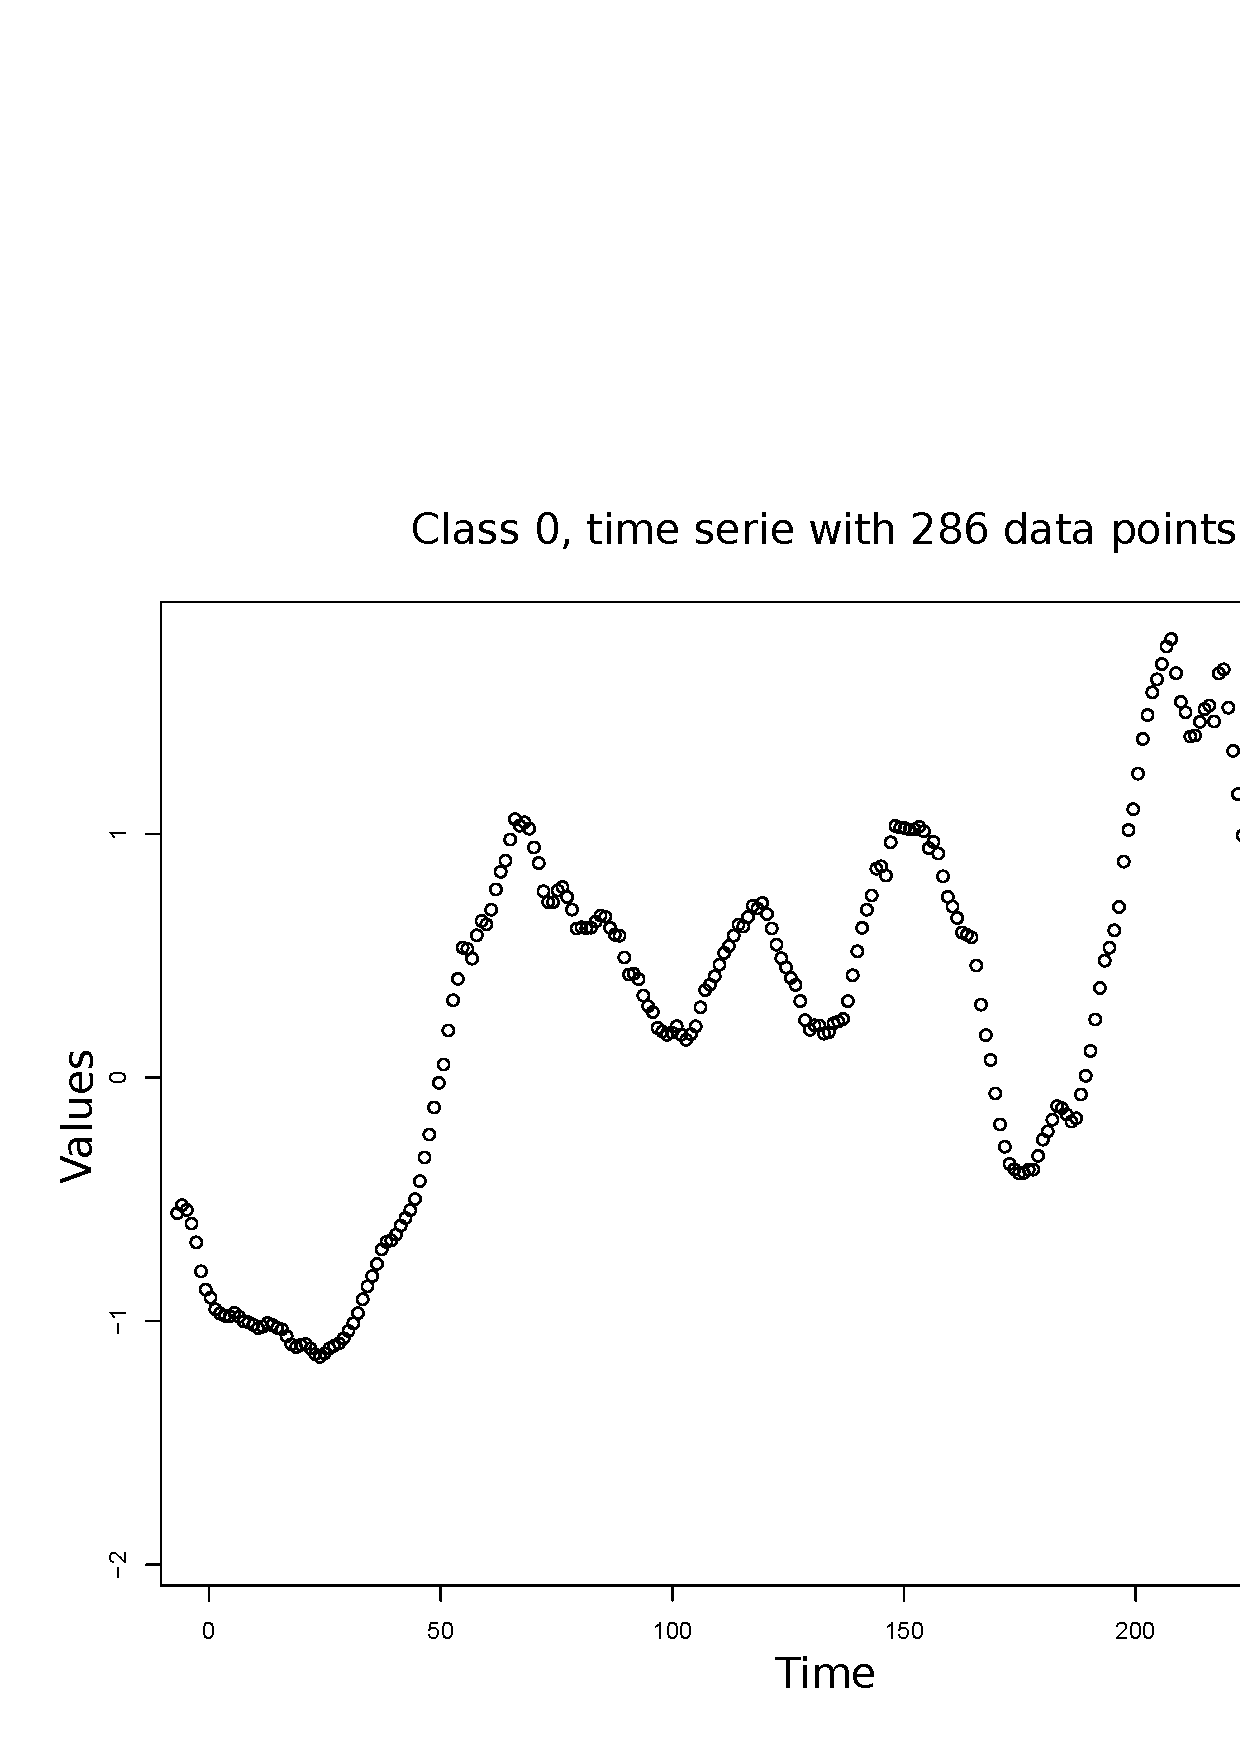
\includegraphics[scale=0.18]{images/coffee_0_ts}
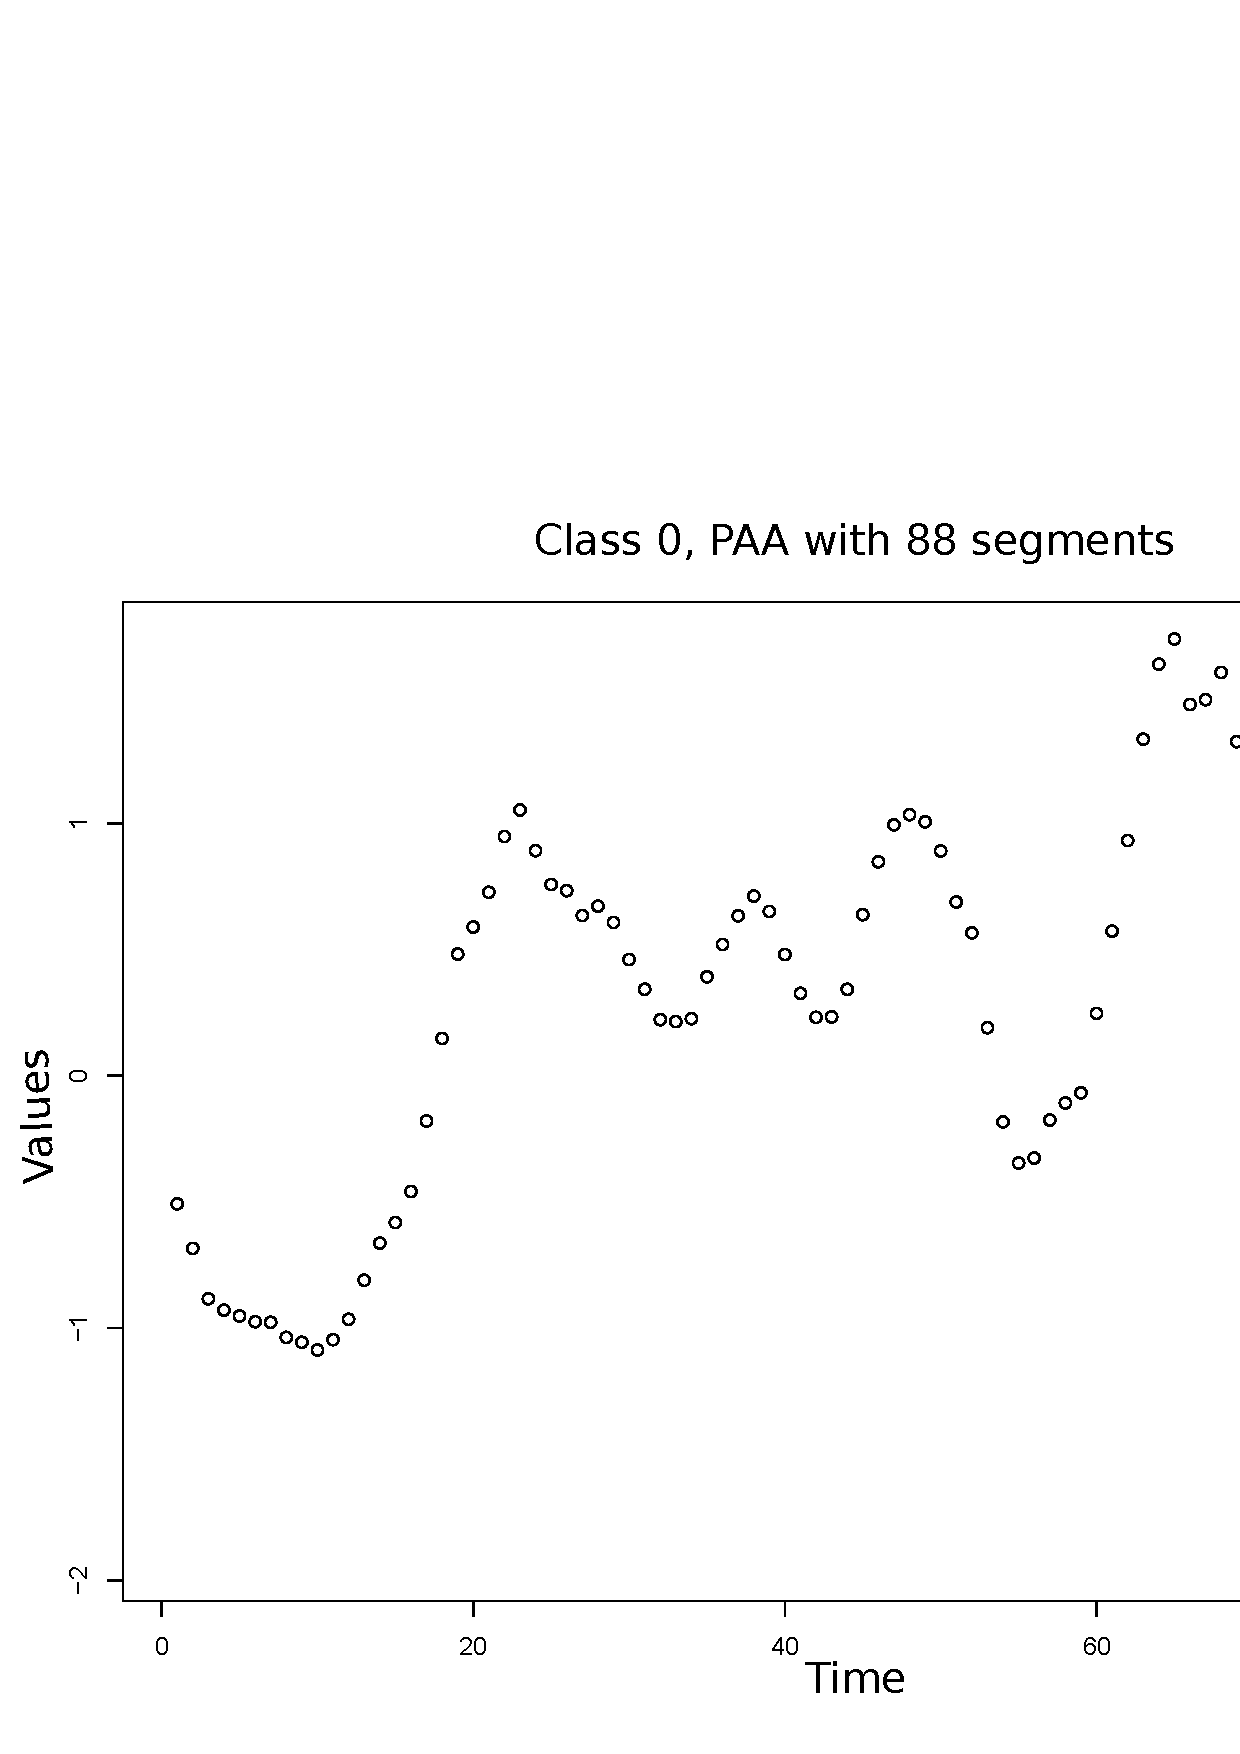
\includegraphics[scale=0.18]{images/coffee_0_paa_88}

%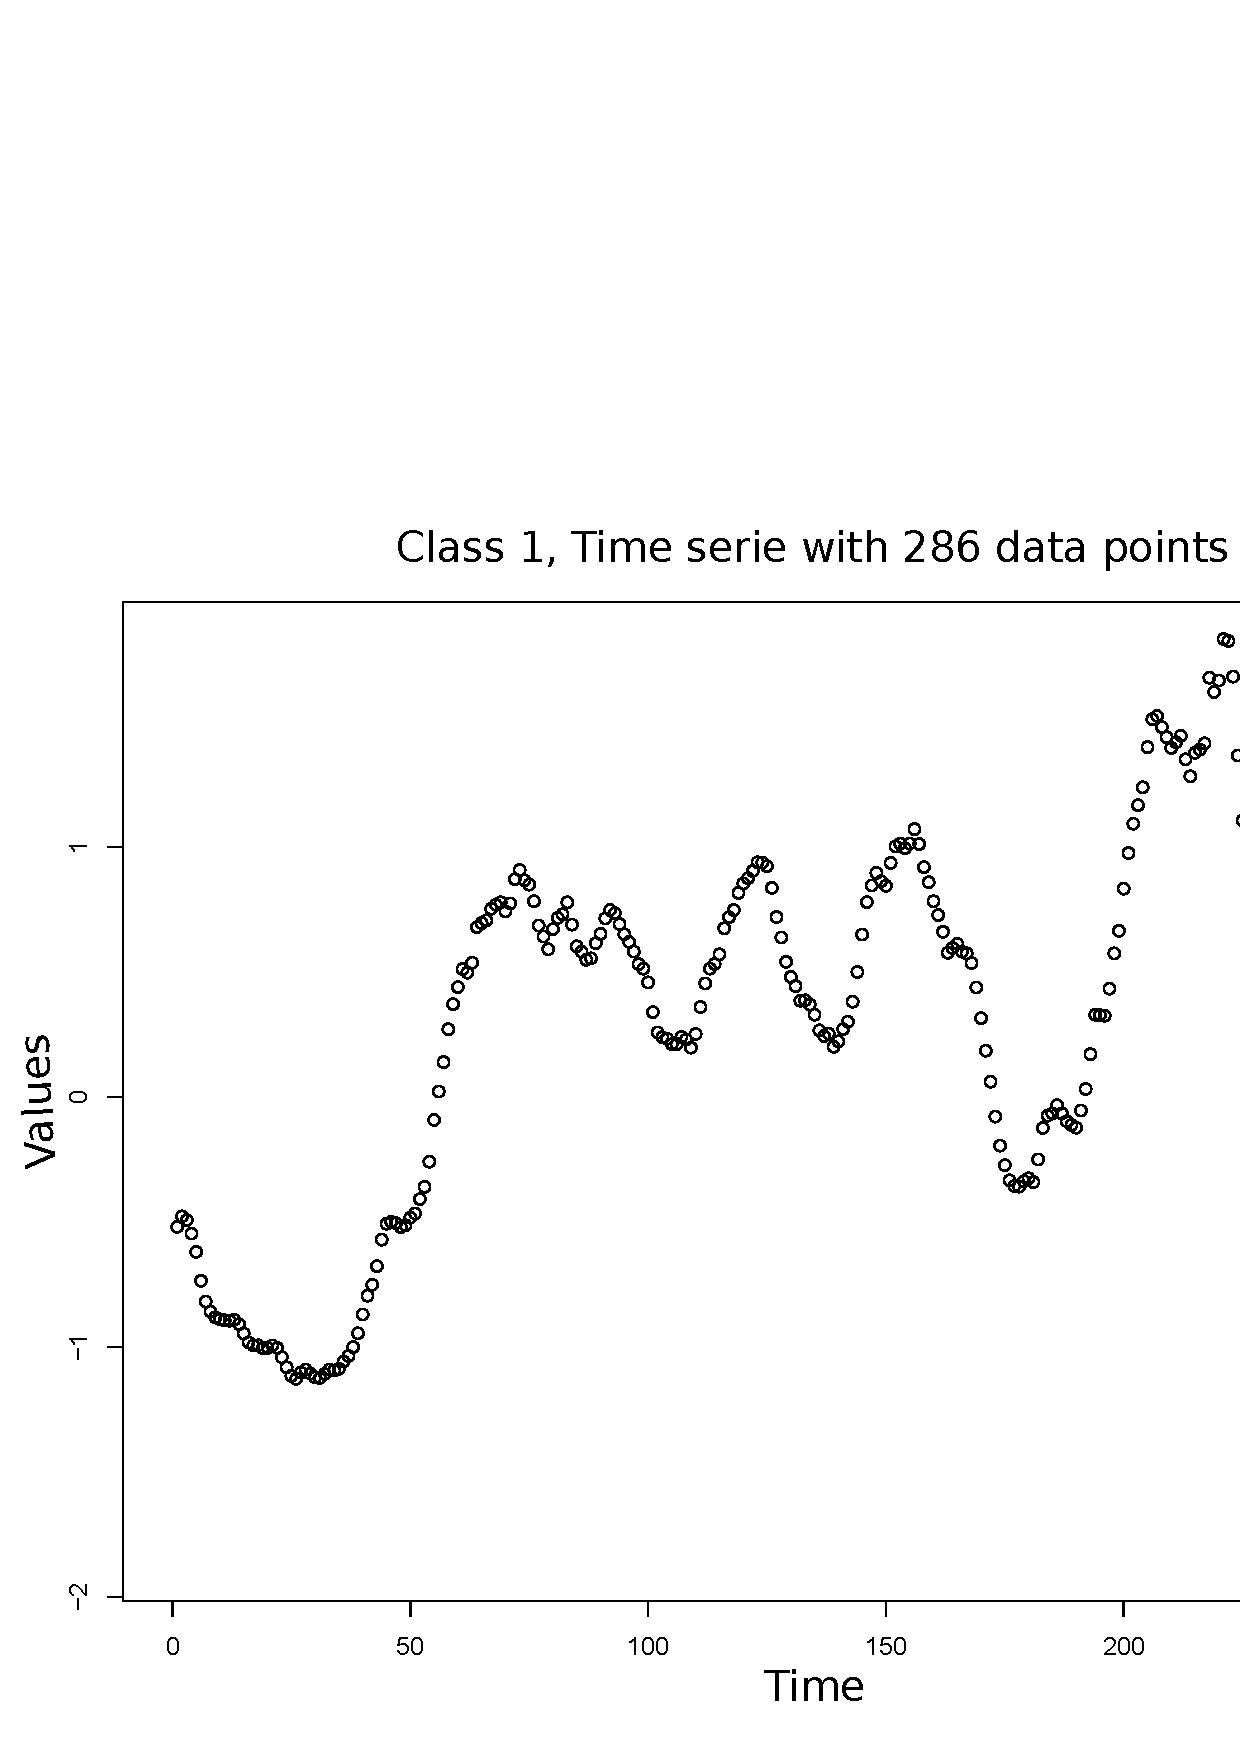
\includegraphics[scale=0.21]{coffee_1_ts}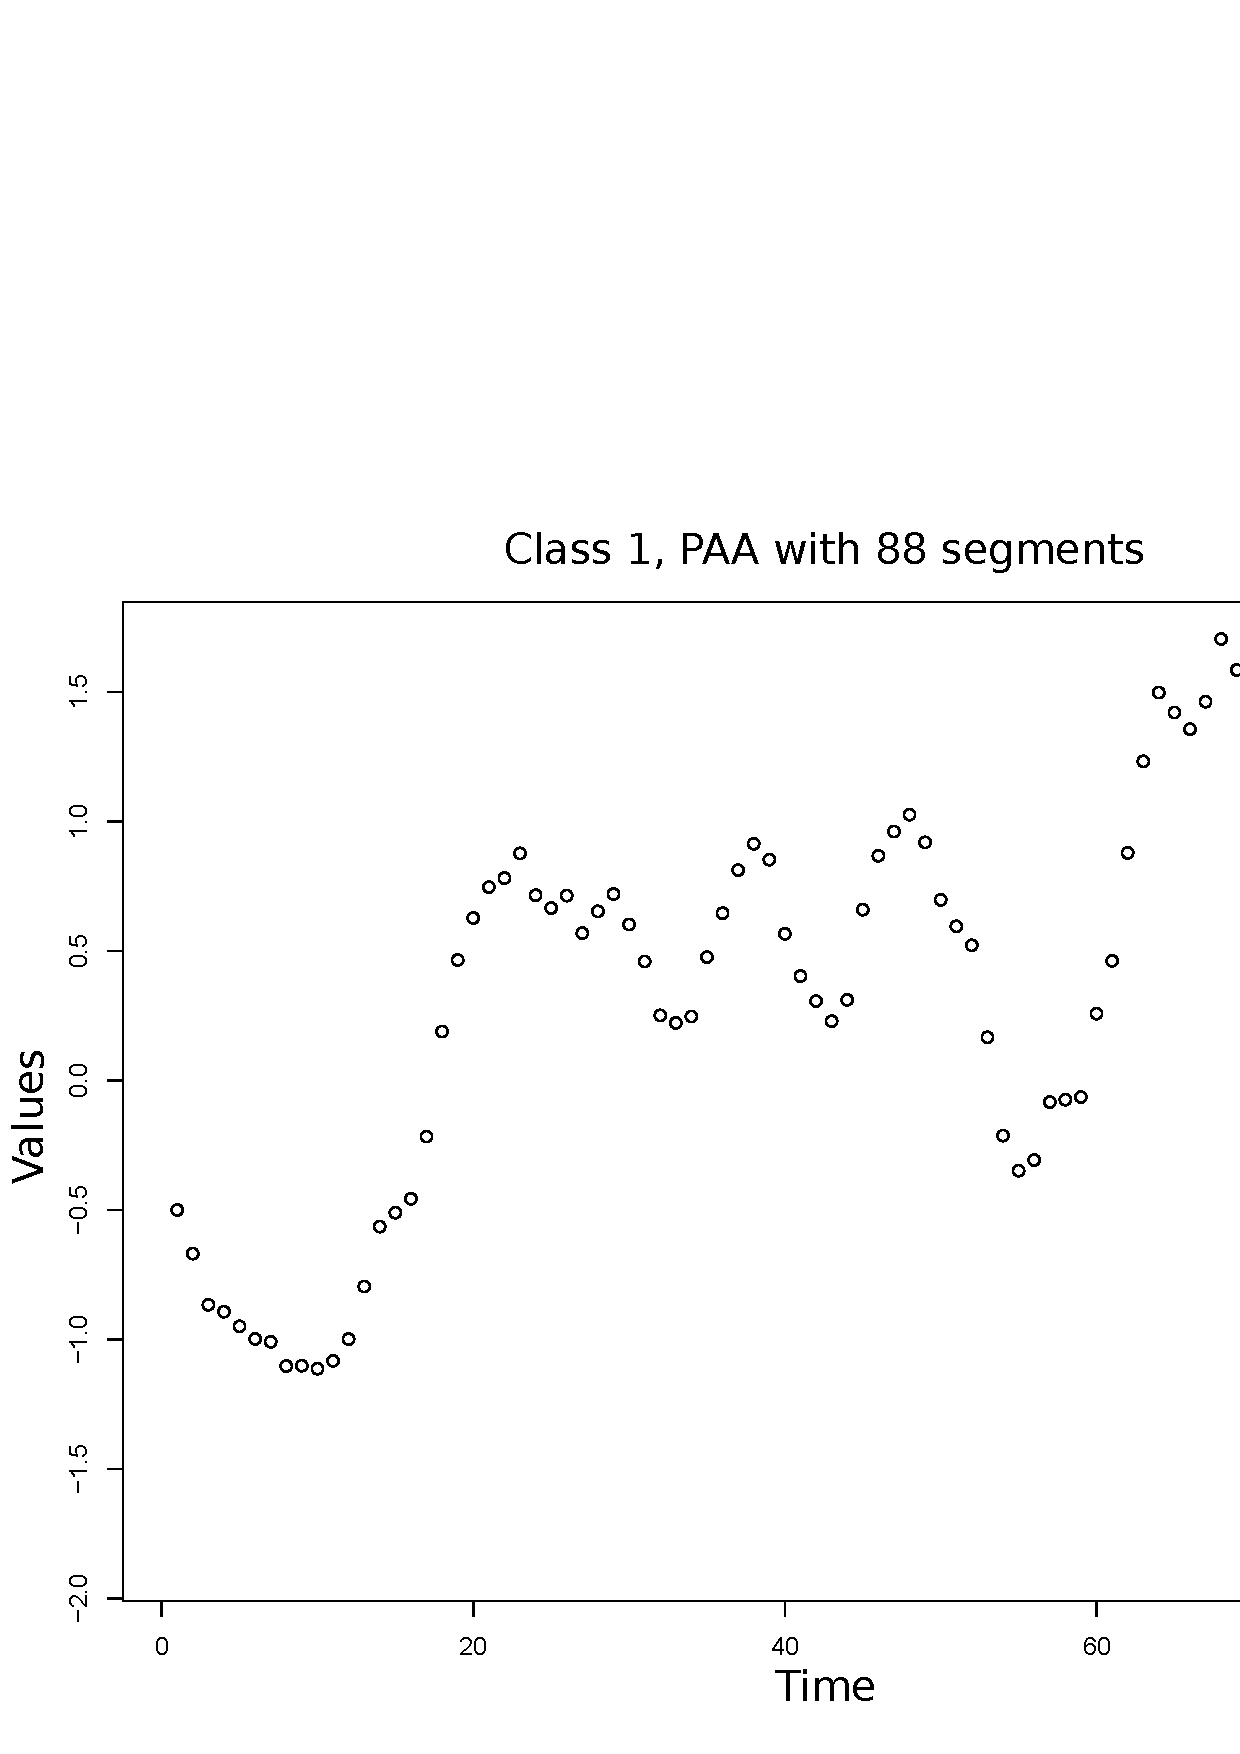
\includegraphics[scale=0.21]{coffee_1_paa_88}

\caption{Coffee dataset time series compression with PAA: original time series
(left) versus PAA represetion using 88 segments (right). The number of segments
is found by FDTW and allow to reduce the length of the time series while retaining the information that it contains.}

\label{coffee}
\end{figure}



\subsection{Classification}
To evaluate the quality of FDTW, we compared its classification errors with that of 35 other classification algorithms \cite{bagnall2016great} of the literature on 84 datasets of UCR archive{{}}.
The classification error  was calculated  based on the holdout model evaluation. FDTW used
the training set to find the number of segments $N$ using 3-fold cross-validation. If two
numbers of segments $N_1$ and $N_2$ are associated with the same classification error, we retain the
largest. The performances of the algorithms are compared using 
the Nemenyi test that compares all the algorithms pairwise and  provides an intuitive way to
visualize the results (Fig. \ref{cd2}). The Nemenyi test allows ranking the classification algorithms according to their average accuracy on 84 datasets.


The value of the segment number N found on the training set may in some cases not be appropriate for the testing set. We speak of an error of generalization which is due to the representativeness of the training set. Thus, FDTW obtains good results on the simulated data sets 3rd / 37 algorithms in terms of average accuracy (Fig. \ref{cd2}) because the data of the training set and the testing set are generated by the same models.

\begin{figure}
\centering
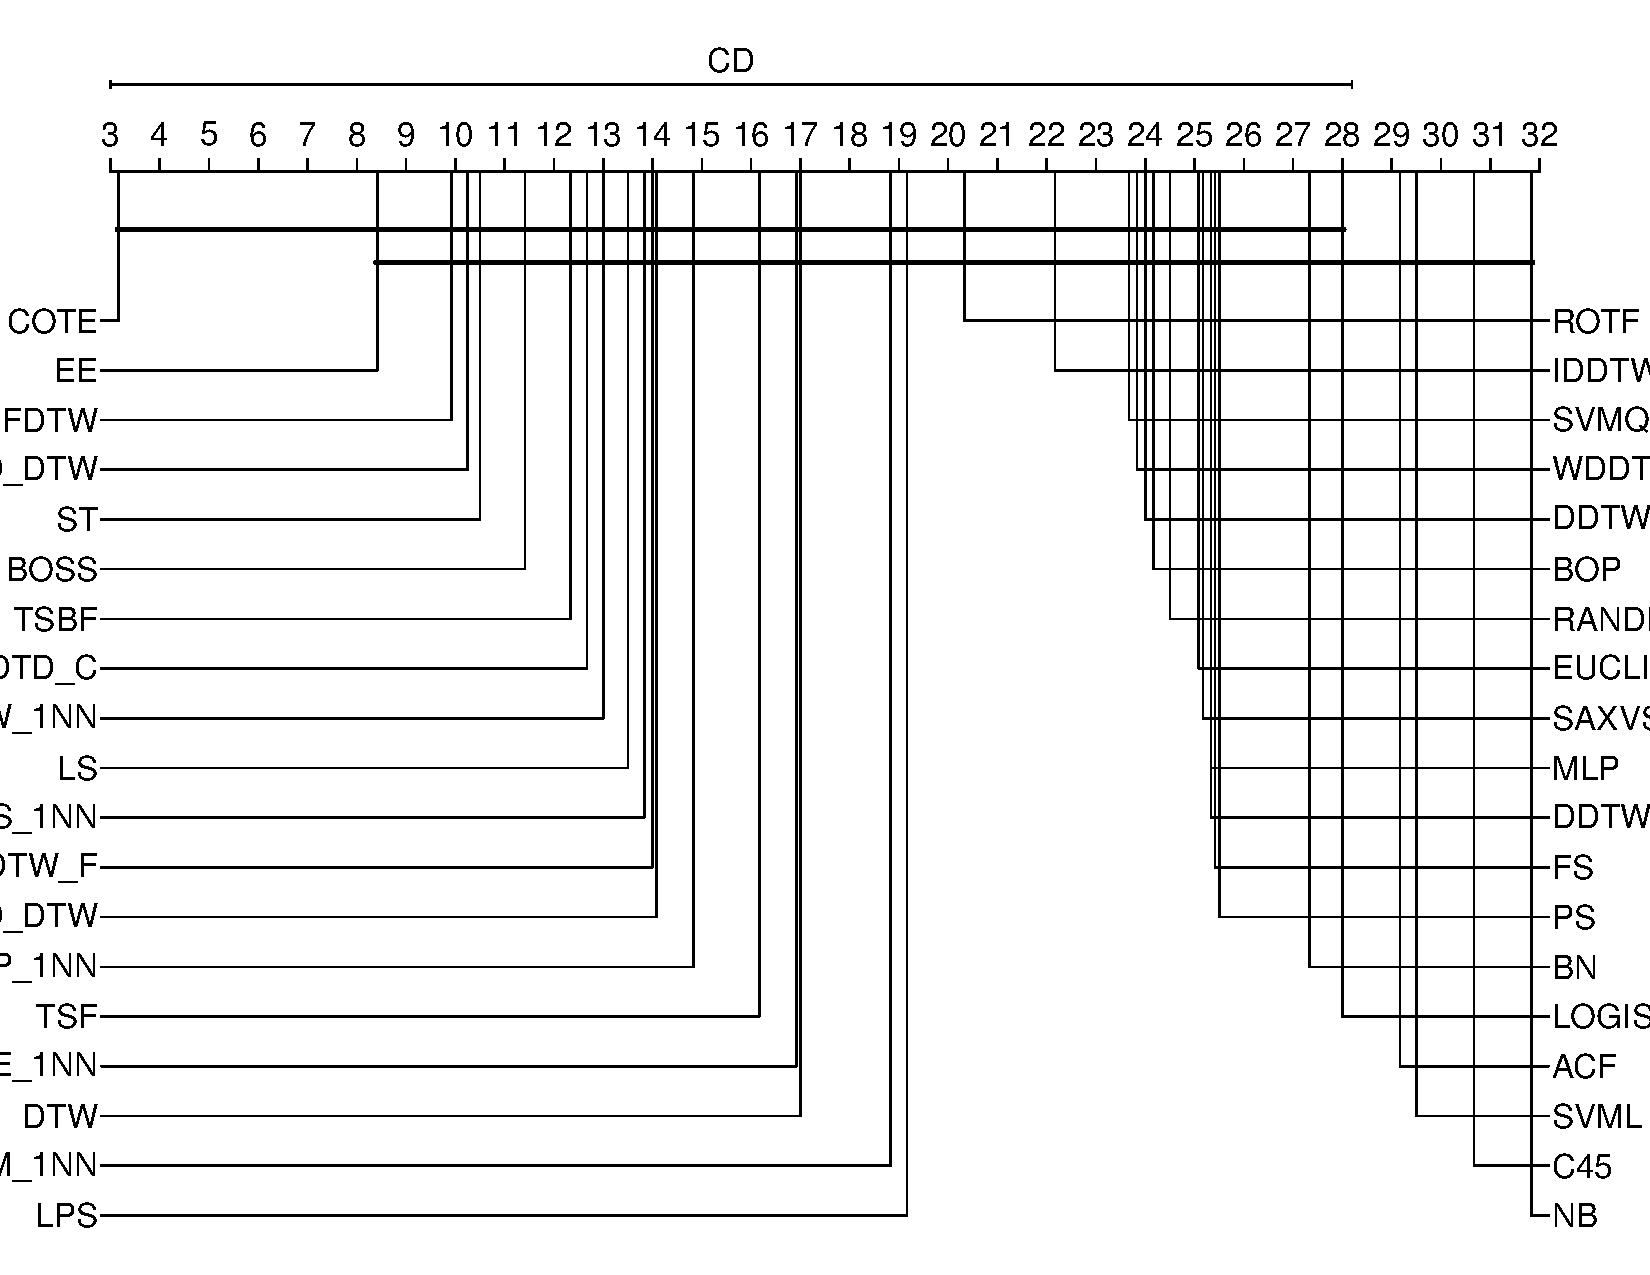
\includegraphics[scale=0.23]{images/cd1}
\caption{Critical difference diagram for FDTW and $36$ other classification algorithms on 6 simulated datasets.}

\label{cd2}
\end{figure}



However, to evaluate the significance of the difference between the classification algorithms on 84 datasets, we use the Wilcoxon signed rank test with continuity correction which has more statistical power.The results of these experiments are summarized below. 

The experiments show that despite data compression : 
\begin{itemize}
  \item  FDTW have better performance than Naive Bayes (NB), C45,  logistic regression (Logistic), BN;
  \item FDTW has similar performance to that of 26 other algorithms in the literature, namely : SVMQ, RANDF, ROTF, MLP, EUCLIDEAN\_1\_NN, DDTW\_R1\_1NN, DDTW\_RN\_1NN, ERP\_1NN, LCSS\_1NN, MSM\_1NN, TWE\_1NN, WDDTW\_1NN, WDTW\_1NN, DD\_DTW, DTD\_C, LS, BOP, SAXVSM, TSF, TSBF, LPS, PS, CID\_DTW, SVML, FS, ACF;
  \item DTW\_F, Shapelet Transform (ST), BOSS, Elastic Ensemble (EE) and COTE perform better overall than FDTW.
\end{itemize}

This demonstrates its competitiveness. Moreover, FDTW
outperforms the best result reported in the literature on  UWaveGestureLibraryAll dataset (Fig.
\ref{geste}).
The challenge with the UWaveGestureLibraryAll dataset is to recognize the gesture made by a user
from measurements made by accelerometers. As reported here \cite{Bagnall} the best accuracy obtained
on this dataset is 83.44\% with TSBF algorithm. FDTW outperforms this result and allows to obtain \textbf{91.87\%} of accuracy.


\begin{figure}[h]
\center
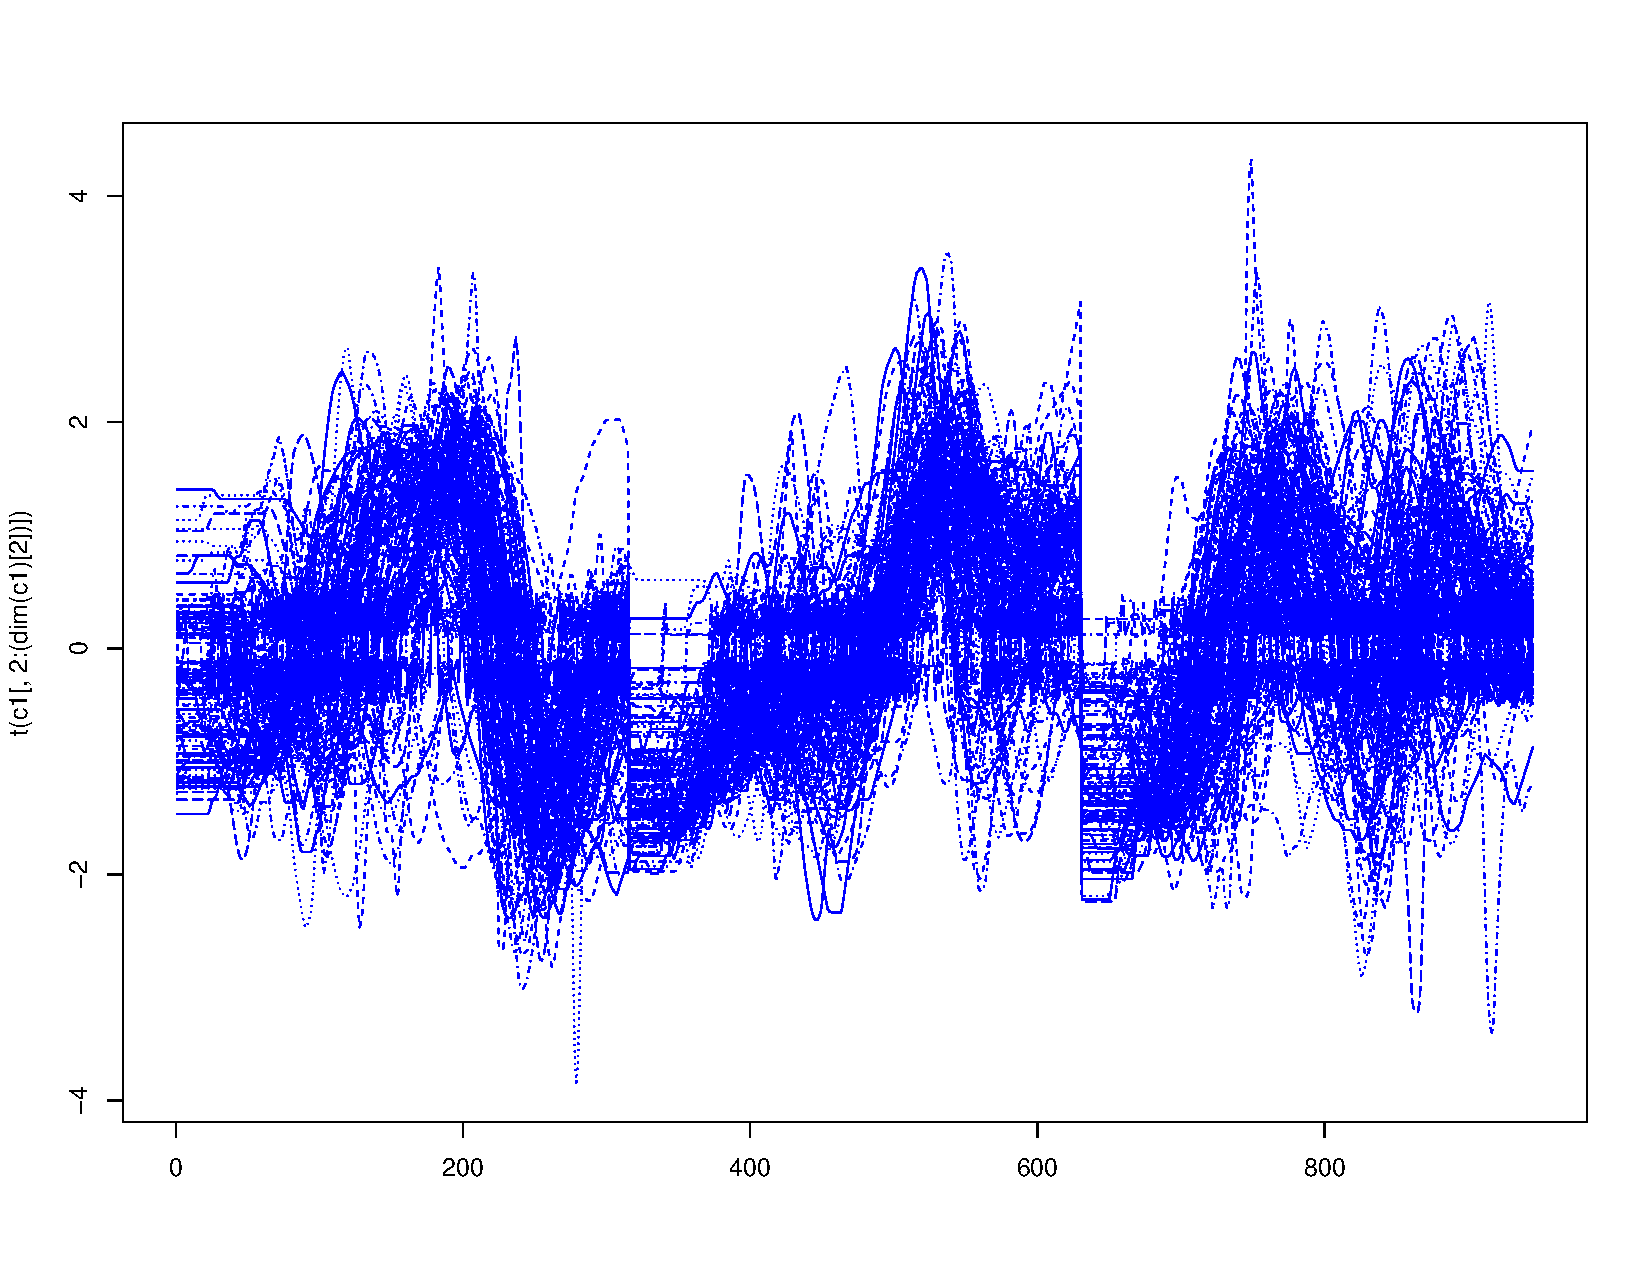
\includegraphics[scale=0.1]{images/c1}
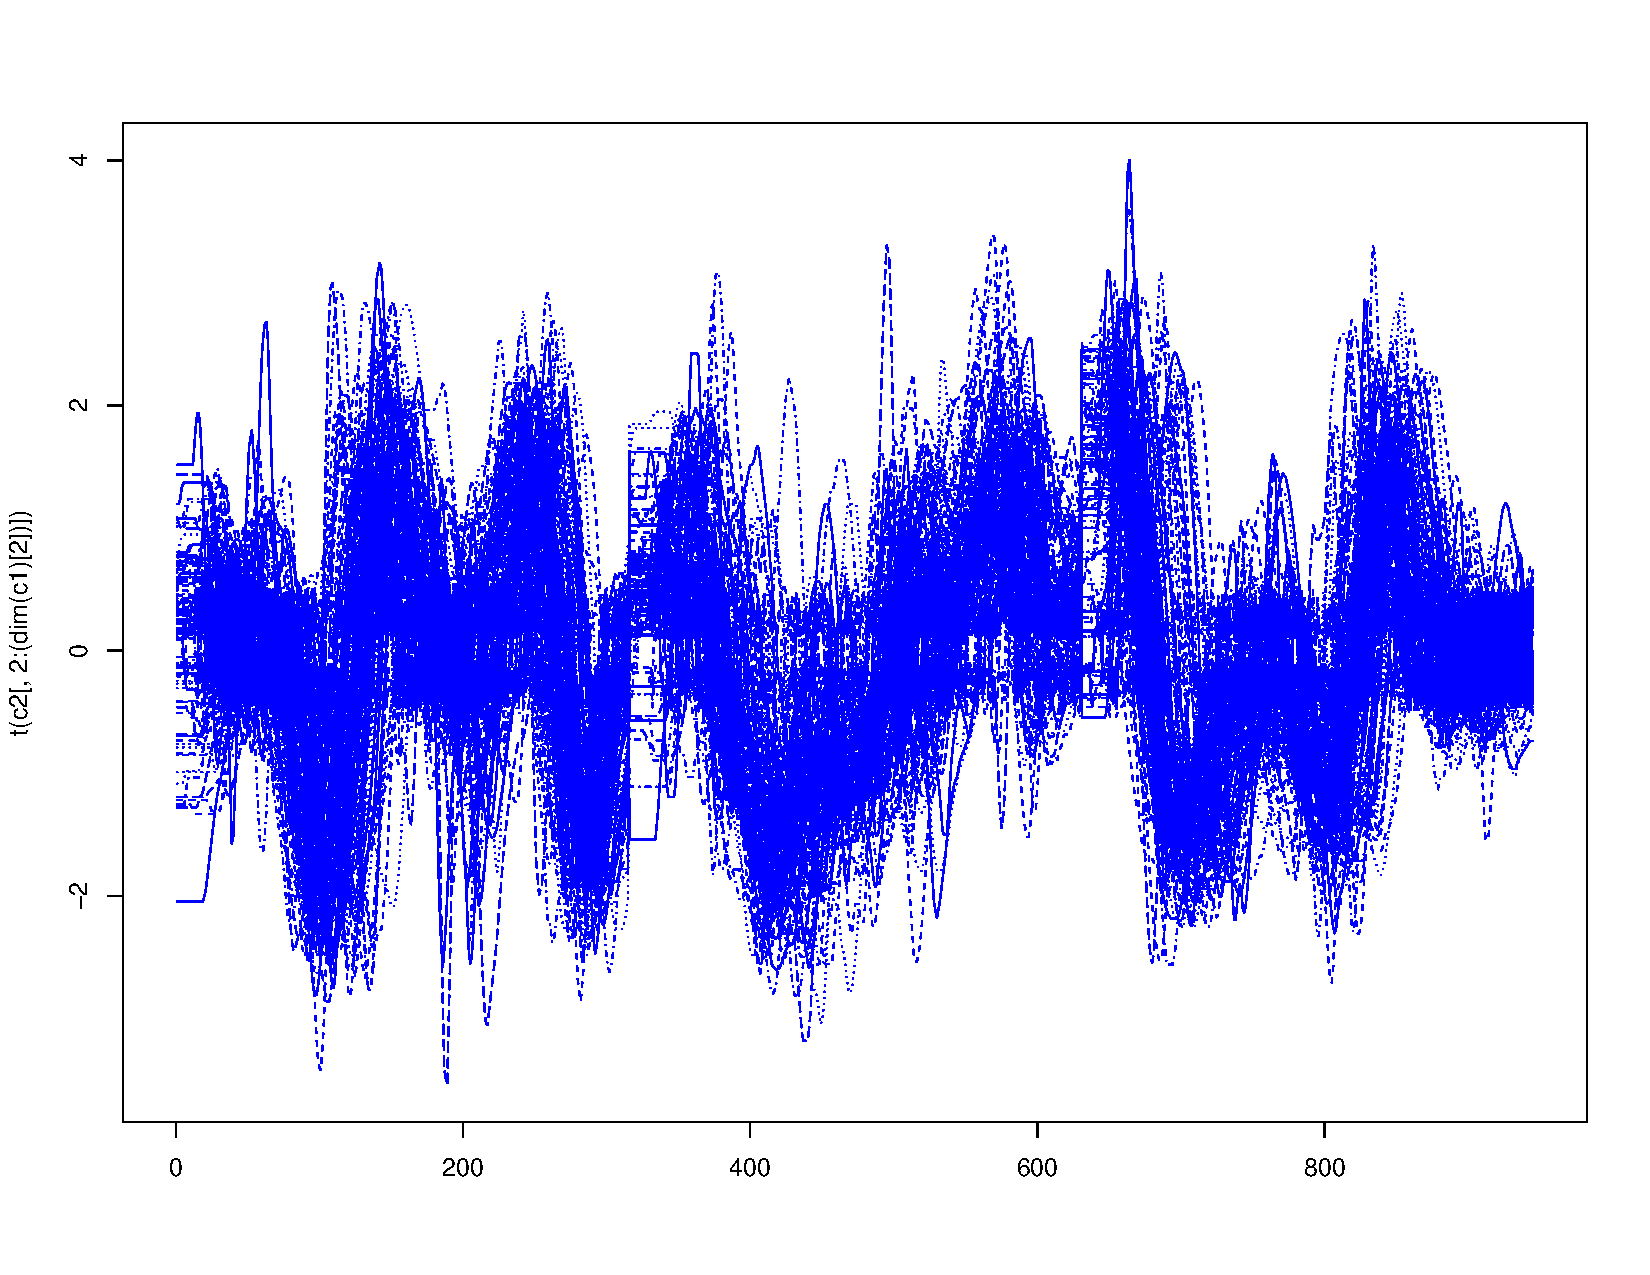
\includegraphics[scale=0.1]{images/c2}
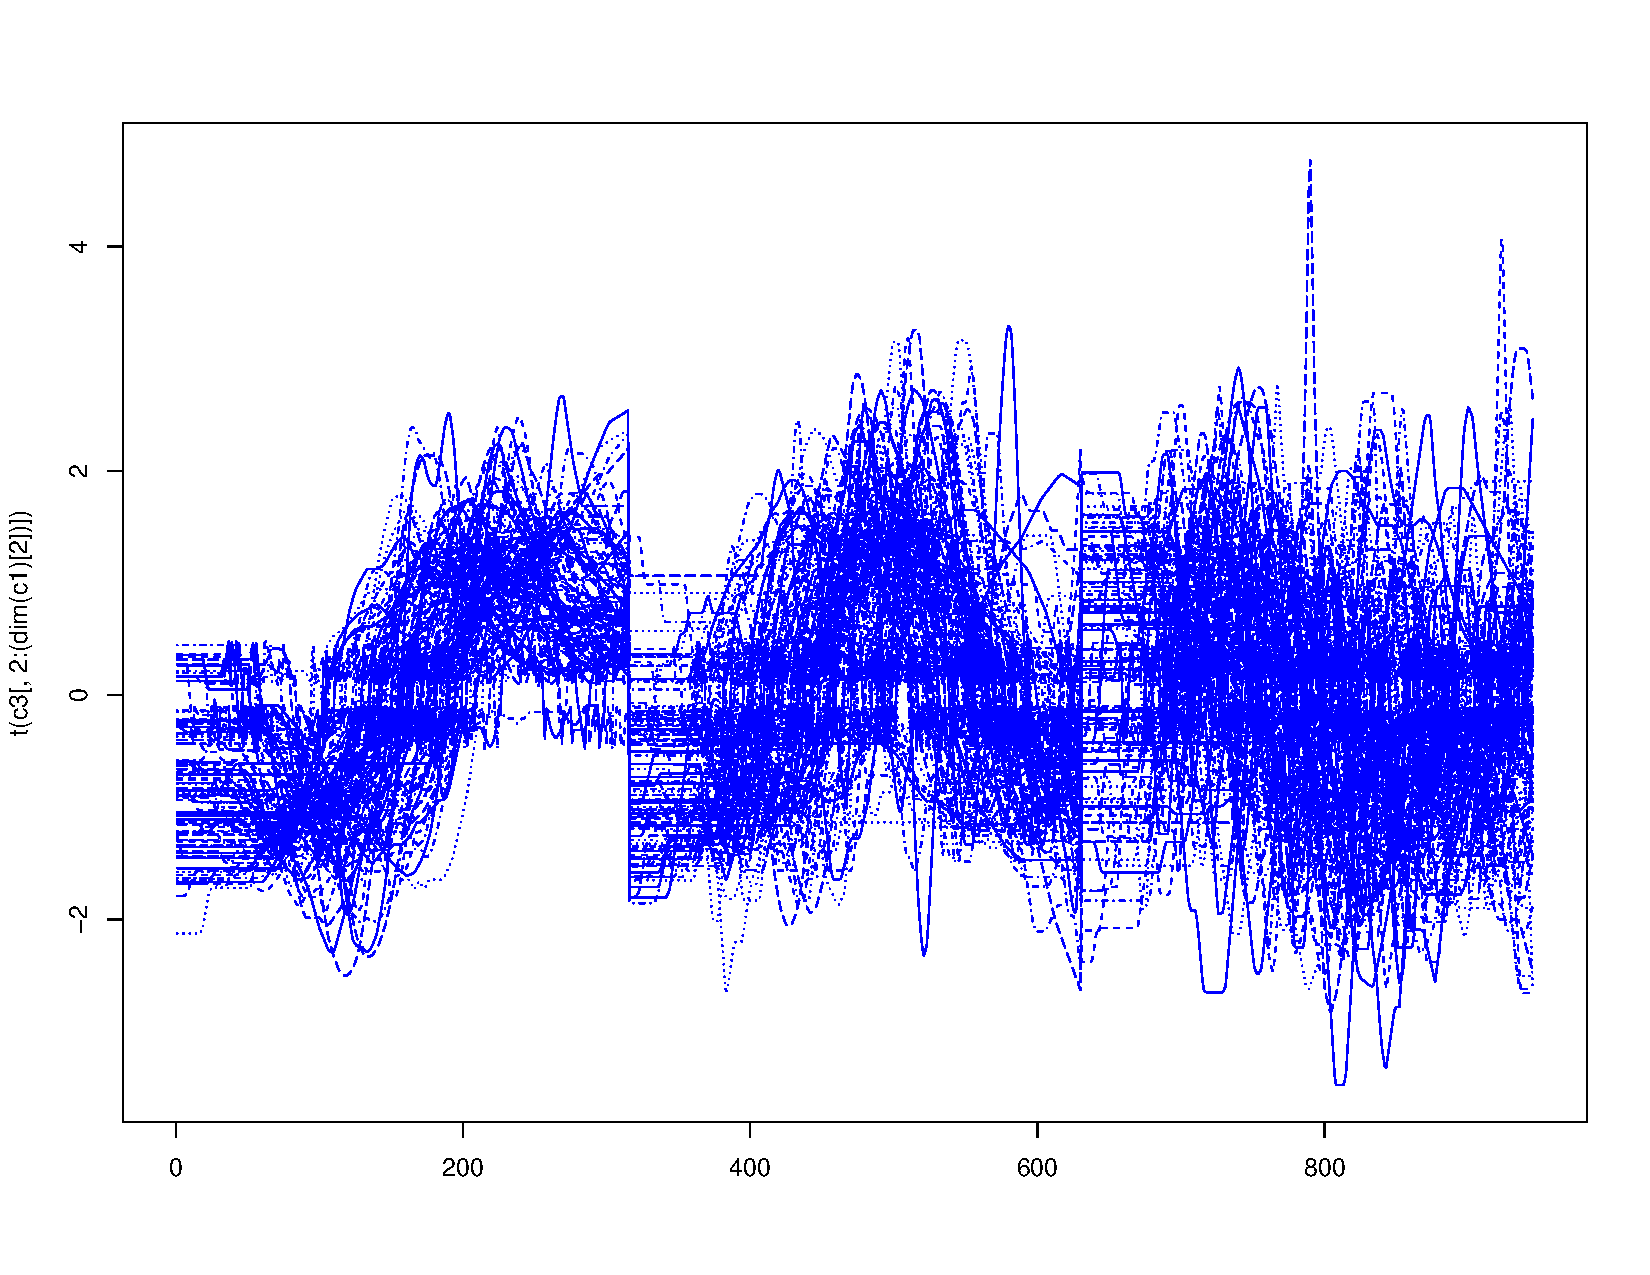
\includegraphics[scale=0.1]{images/c3}
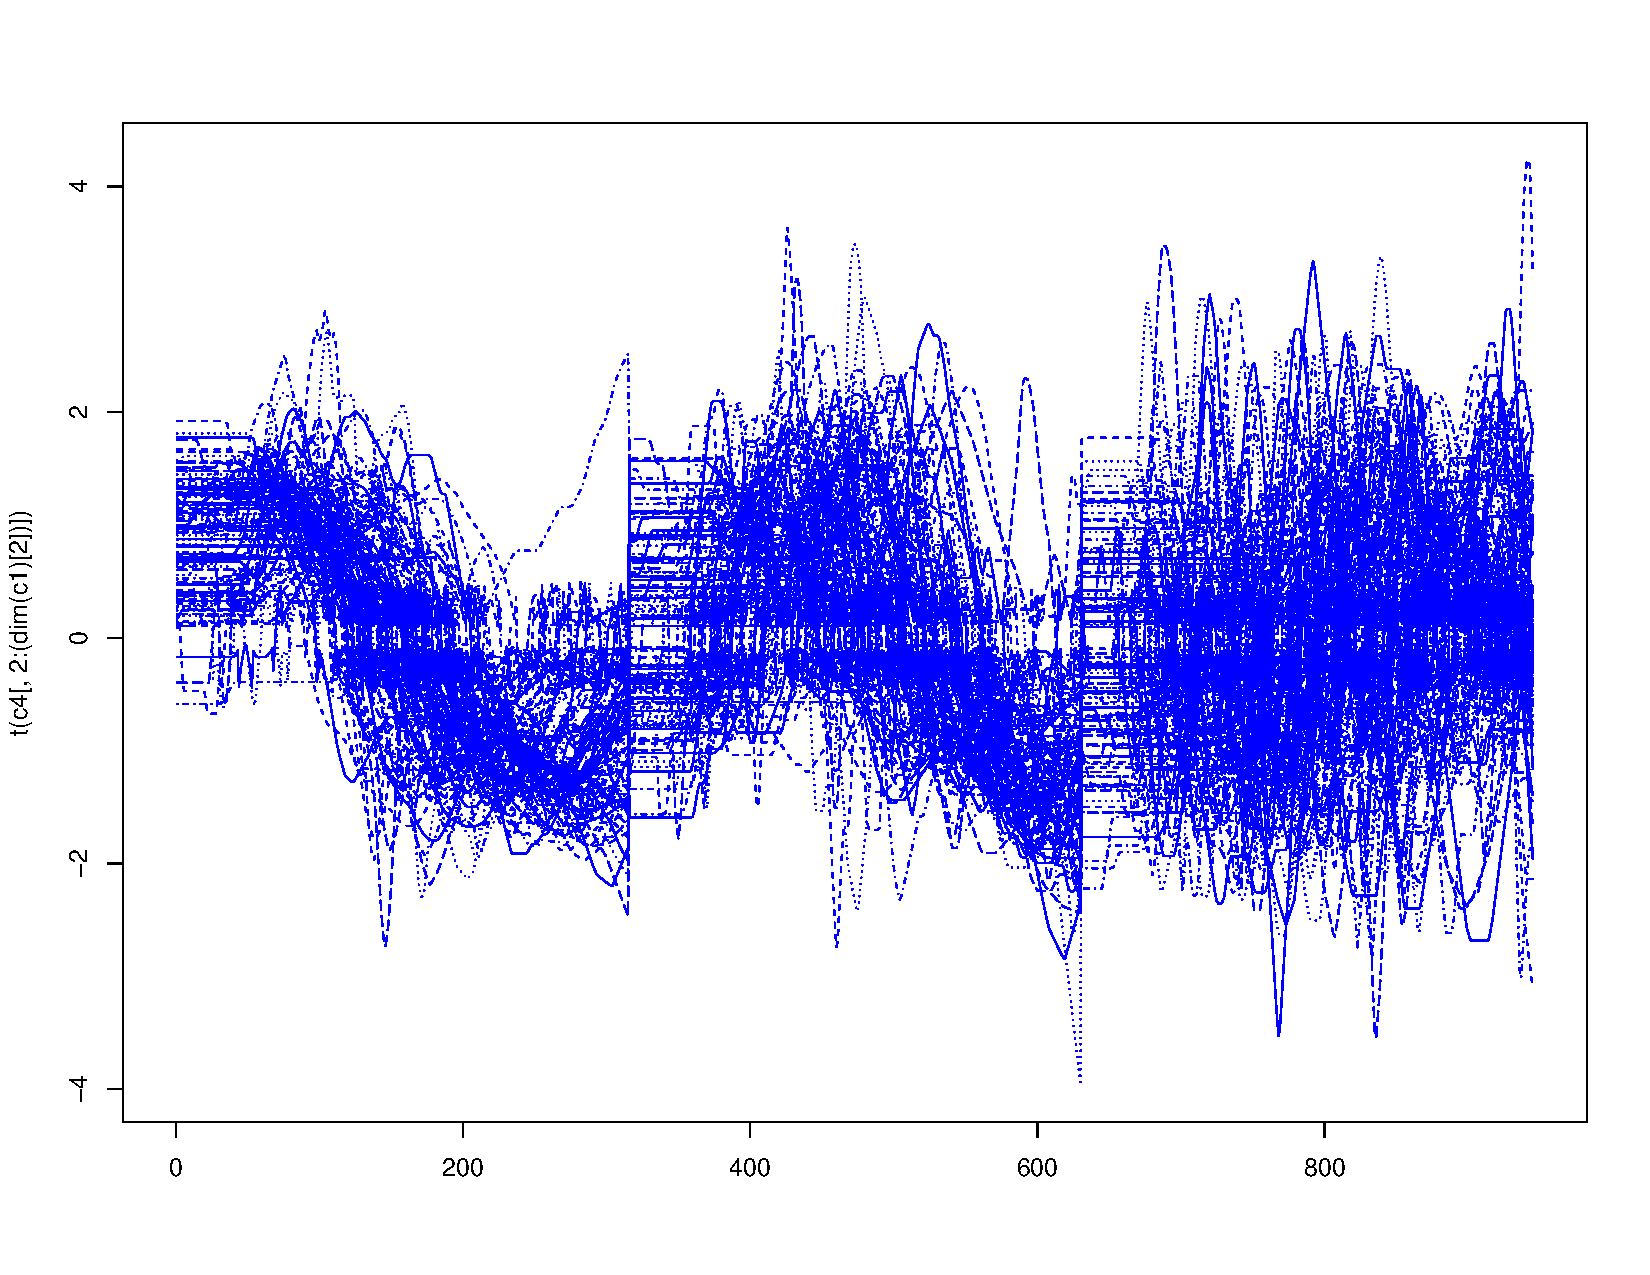
\includegraphics[scale=0.1]{images/c4}
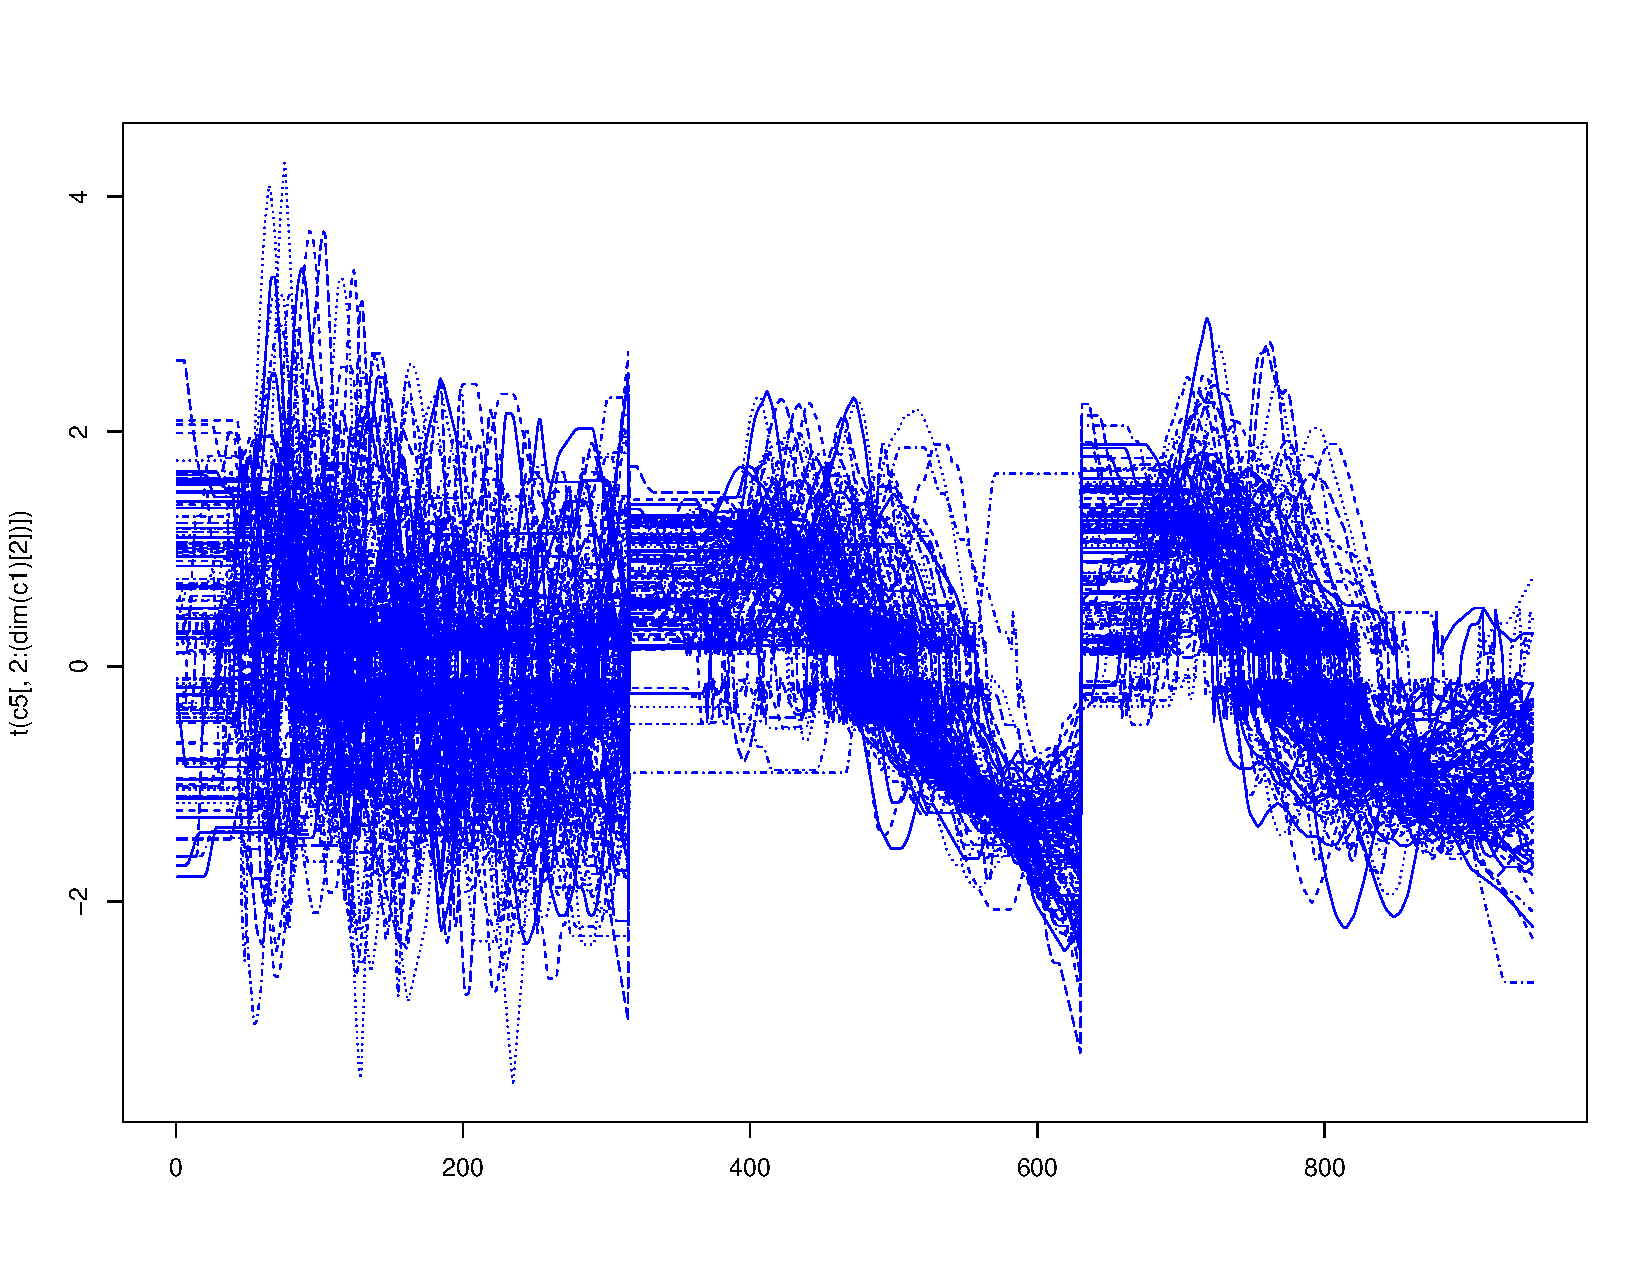
\includegraphics[scale=0.1]{images/c5}
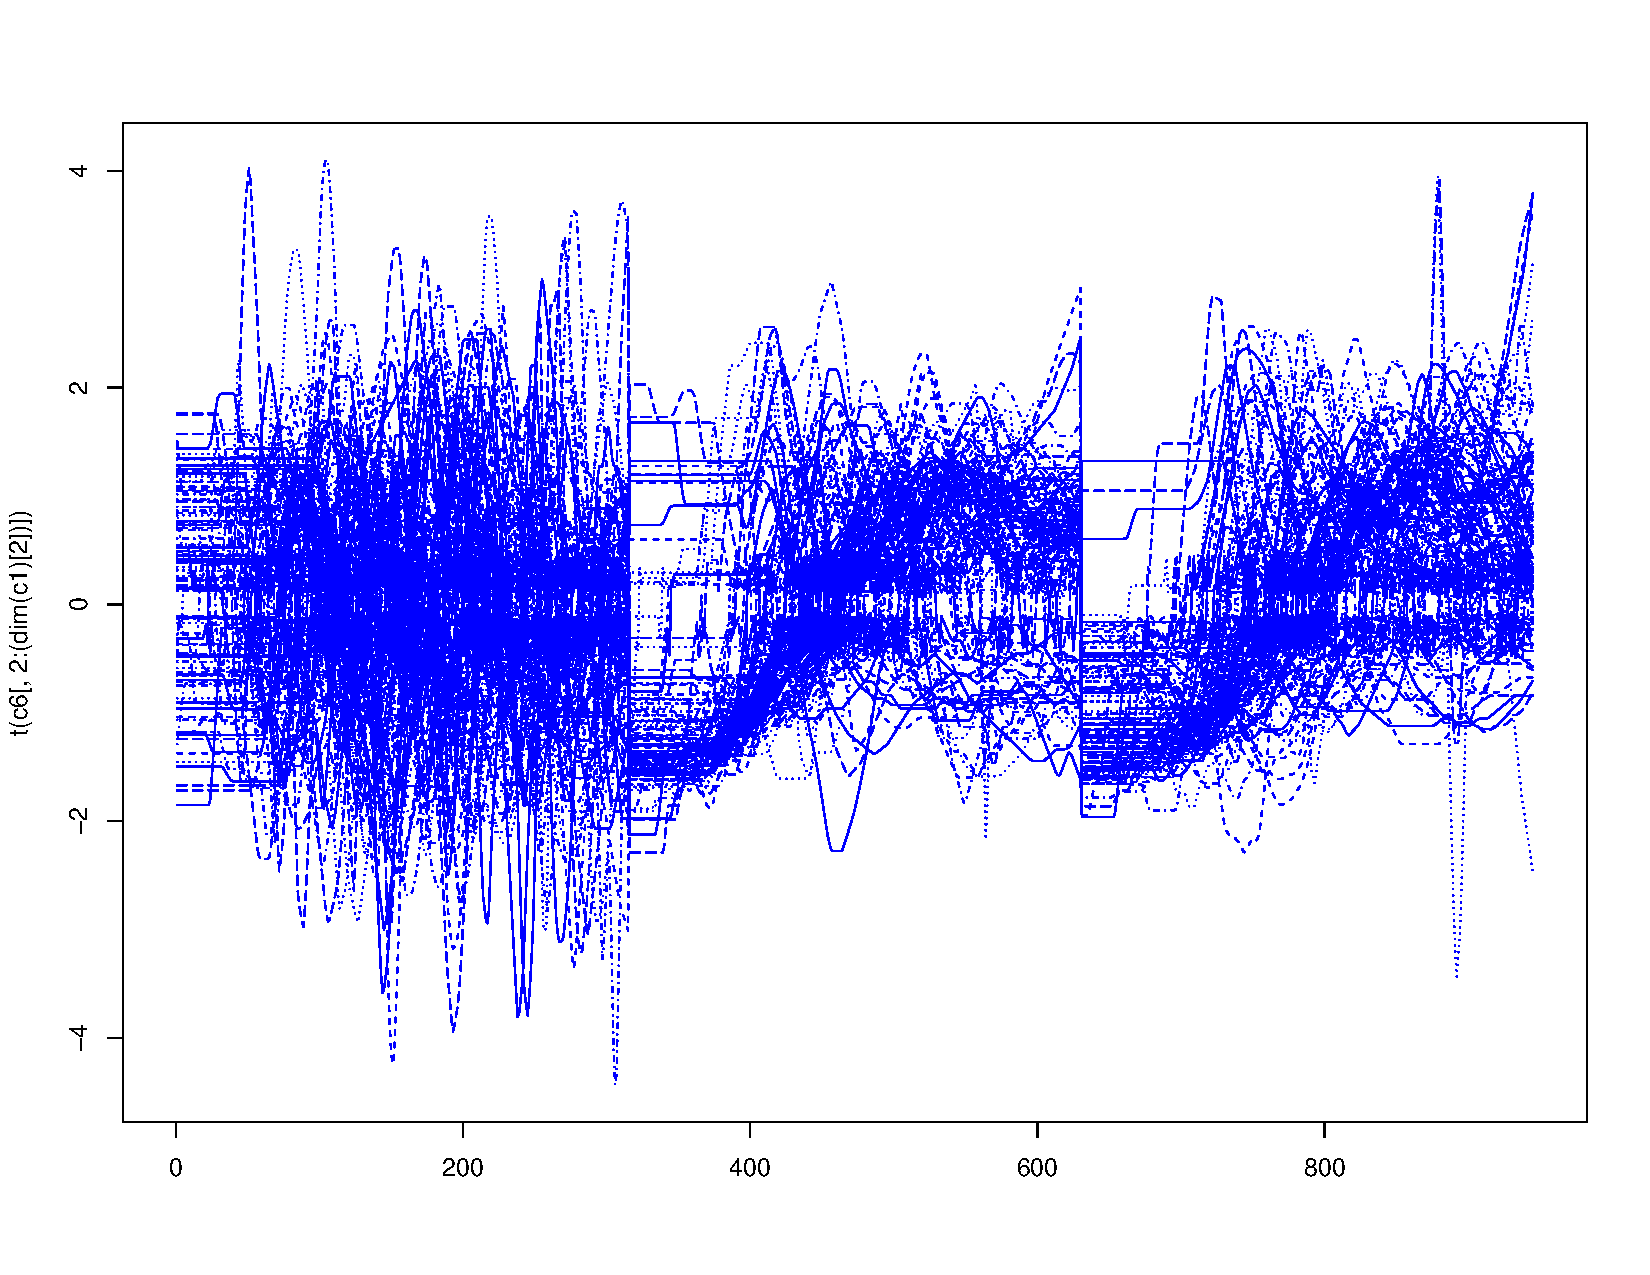
\includegraphics[scale=0.1]{images/c6}
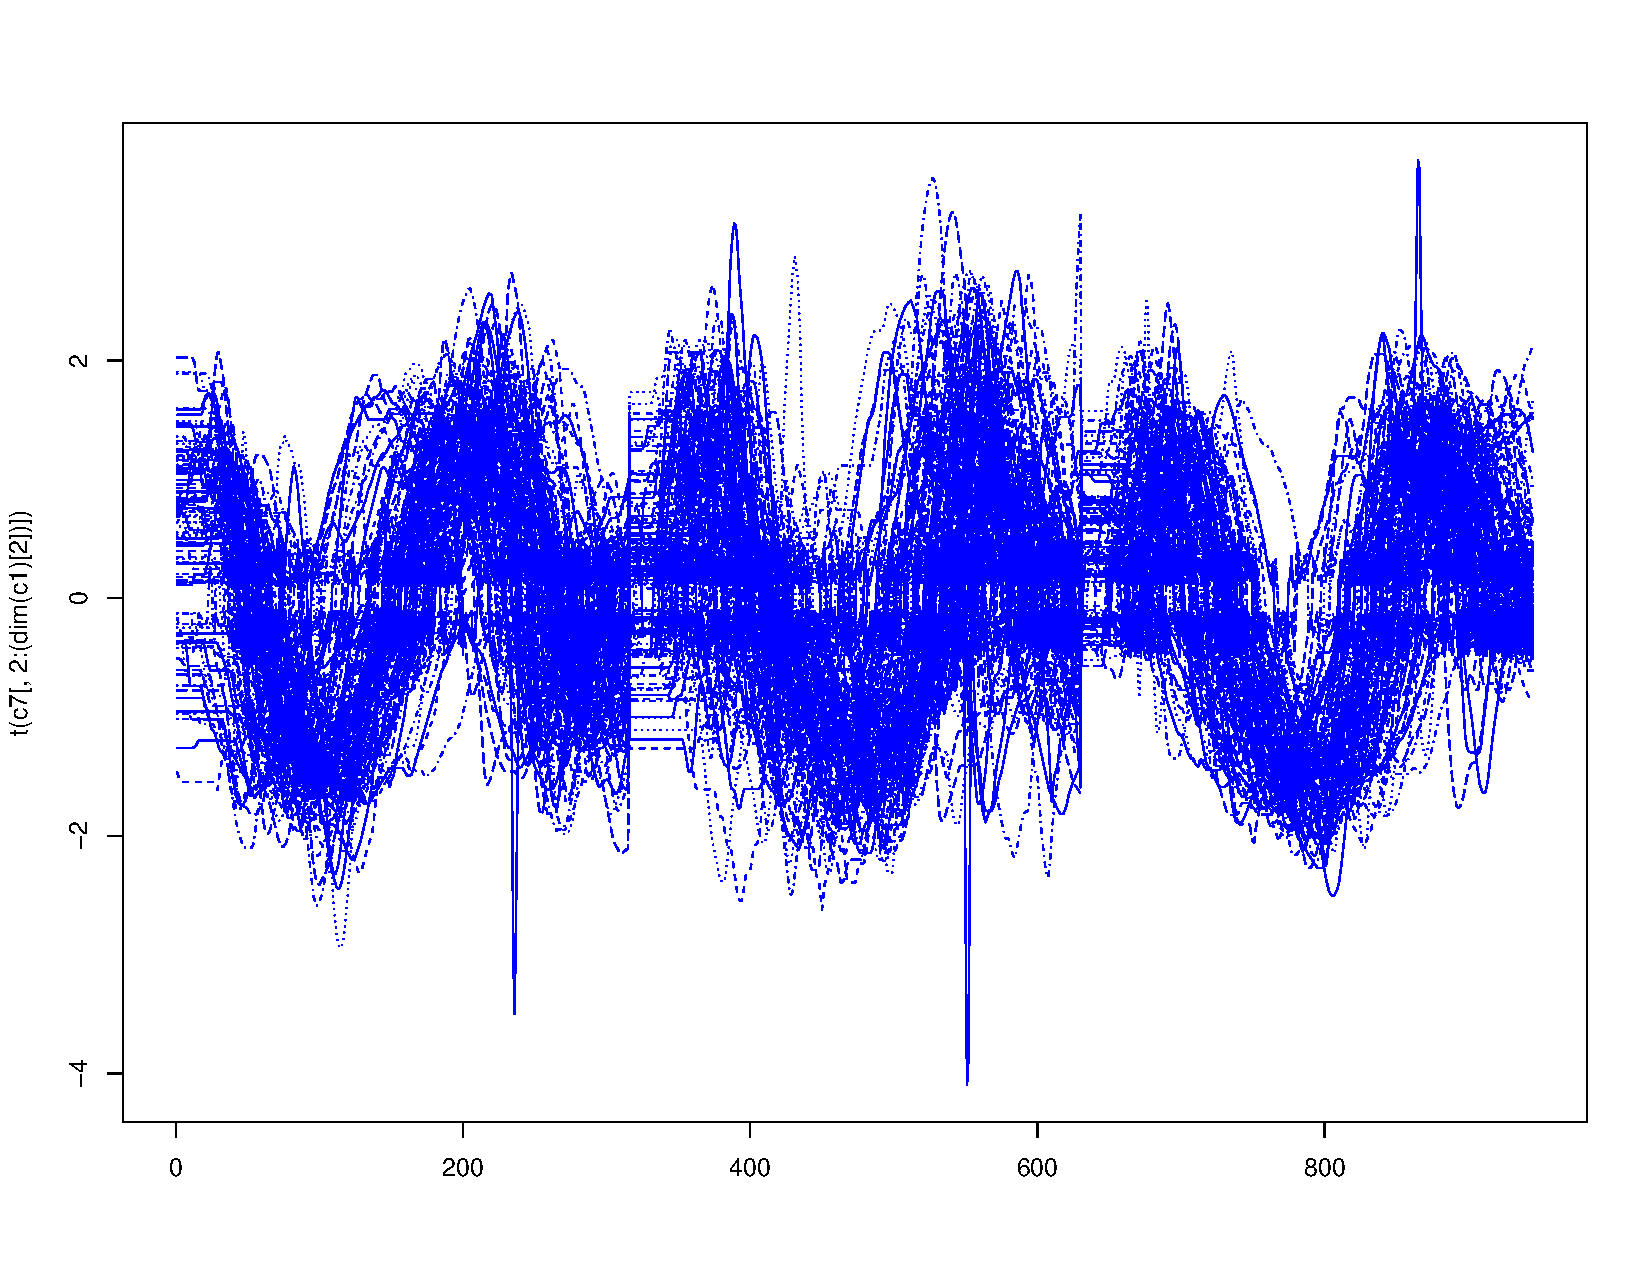
\includegraphics[scale=0.1]{images/c7}
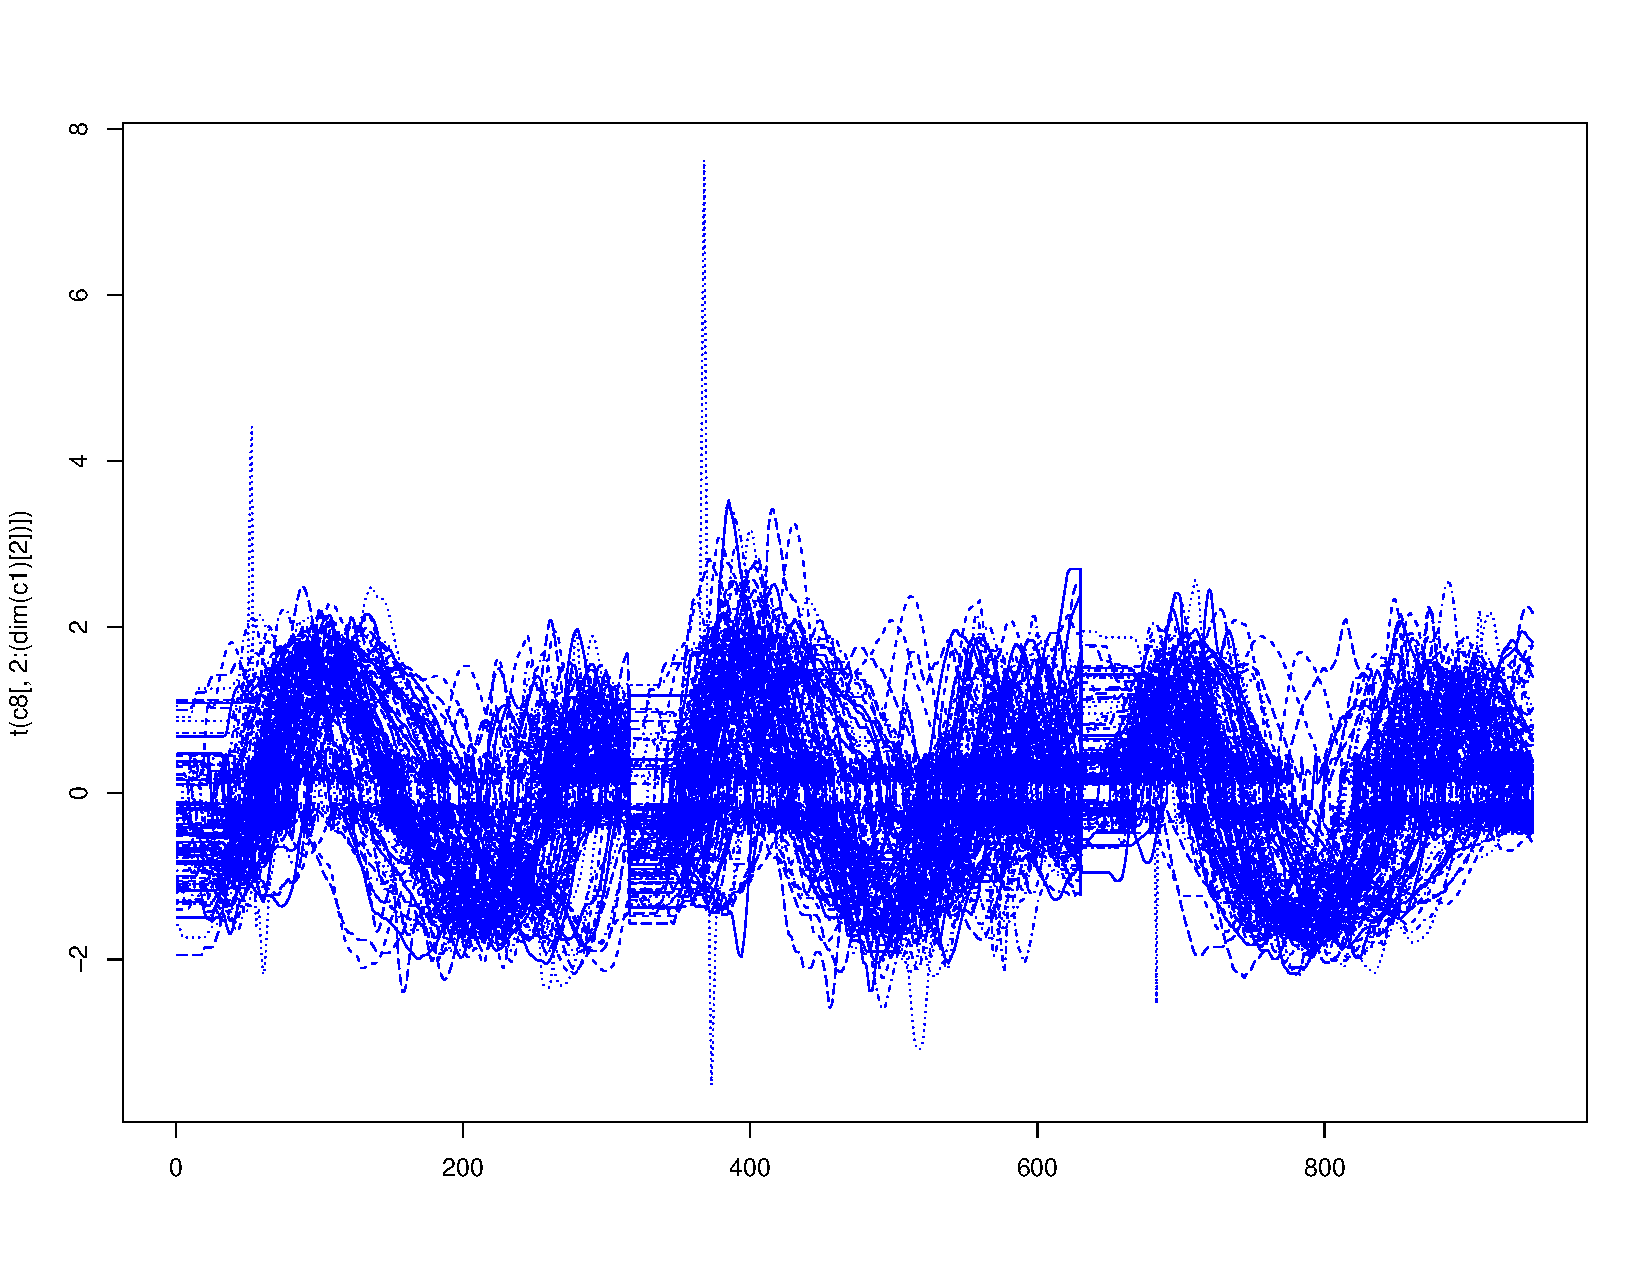
\includegraphics[scale=0.1]{images/c8}

\caption{Eight types of time series corresponding to the vocabulary of 8 gestures.}

\label{geste}
\end{figure}



\section{Conclusion}
\label{sec:4}
Our problem in this paper was to choose an appropriate number of segments to compress time series with PAA in order to improve the alignment with DTW. To achieve this goal we proposed a parameter Free heuristic named FDTW with approximate the optimal number of segment to use. The experiments show that our heuristic increased the quality of alignment of time series with especially on synthetic datasets where DTW associated with PAA perform better than any other variant of DTW on a classification task and was rank 3/37 behind two ensemble classification algorithms COTE and EE. This work allows reducing the storage space and the processing time of time series while increasing the quality of the alignment of DTW. 
The same strategy presented in FDTW can be used to find the number of segments to be considered for the indexation and for symbolic representations of time series like SAX \cite{lin2003symbolic}, ESAX \cite{lkhagva2006extended}, SAX-TD \cite{sun2014improvement}.

\chapter[Uncertain time series u-shapelet discovery]{Frobenius correlation based u-shapelets discovery for time series clustering}

\begin{abstract}
An u-shapelet is a sub-sequence of a time series used for clustering a time series dataset. The purpose of this paper is to discover u-shapelets on uncertain time series. To achieve this goal, we propose a dissimilarity score called FOTS whose computation is based on the eigenvector decomposition and the comparison of the autocorrelation matrices of the time series. This score is robust to the presence of uncertainty; it is not very sensitive to transient changes; it allows capturing complex relationships between time series such as oscillations and trends, and it is also well adapted to the comparison of short time series. The FOTS score is  used with the Scalable Unsupervised Shapelet Discovery algorithm for the clustering of 17 datasets, and it has shown a substantial improvement in the quality of the clustering with respect to the Rand Index. This work defines a novel framework for the clustering of uncertain time series.
\end{abstract}

\section{Introduction}
Uncertainty in time series comes from several sources.  For instance, to protect privacy, privacy-preserving transformation \cite{papadimitriou2007time, aggarwal2008unifying} deliberately introduce uncertainty to the confidential data before further processing. In a sensor
network, sensor readings are imprecise because of the presence of noise generated either by the equipment
itself or other external influences \cite{cheng2003evaluating}. Ignoring the uncertainty of the data
can lead to rough or inaccurate conclusions, hence the need to implement uncertain data management techniques. 


Several recent studies have focused on the processing of uncertainty in data mining. Two main approaches allow to take uncertainty into account in data mining tasks: either it is taken into account during the comparison by using appropriate distance functions \cite{Rizvandi2013, Hwang2014, Rehfeld2014, Orang2014, Wang2015, Orang2017}, or its impact is reduced by transformations performed on the data
\cite{Orang2015}.This latter strategy is used natively by the u-shapelet algorithm.

\subsection{U-shapelets algorithm for clustering Uncertain Time Series }

U-shapelets clustering is a framework introduced by\cite{zakaria2012clustering} who suggested clustering time series from the local properties of their sub-sequences rather than
using their global features of the time series \cite{zhang2016unsupervised}. In that aim, u-shapelets clustering first seeks a set of sub-sequences characteristic of the different categories of time series and classifies a time series according to the presence or absence of these typical sub-sequences in it. 

Clustering time series with u-shapelets has several advantages. Firstly, u-shapelets clustering is defined for datasets in which  time series have different lengths, which is not the case for most techniques described in the literature. Indeed, in many cases, the equal length assumption is implied,
and the trimming to equal length is done by exploiting expensive human skill \cite{ulanova2015scalable}.  Secondly, u-shapelets clustering is much more expressive regarding representational power. Indeed, it allows clustering only time series that can be
clustered and do not cluster those that do not belong to any cluster.

Furthermore, it is very appropriate to use u-shapelets clustering with uncertain time series because it can ignore irrelevant data and thus, reduce the adverse effects of the presence of uncertainties in the time series. Despite this advantage, it is highly desirable to take into account the adverse impact of uncertainty during u-shapelet discovery.

\subsection{Uncertainty and u-shapelets discovery issue}
Traditional measurement of similarity like Euclidean distance (ED) or Dynamic Time  Warping (DTW) do not always work well for uncertain time series data. Indeed,   they aggregate the uncertainty of each data point of the time series being compared and thus amplify the negative impact of uncertainty. However, ED plays a   fundamental role in u-shapelet discovery because it is used to compute the gap, i.e. the distance between the two groups formed by a u-shapelet candidate. The discovery of u-shapelet on uncertain time series could thus lead to the selection of a wrong u-shapelet candidate or to assign a time series to the wrong cluster.
 
 
 In this study, our goal is to cluster uncertain time series with u-shapelets algorithm. Our work leverages the observation that the use of a dissimilarity function robust to uncertainty could improve the quality of the u-shapelets discovered and thus improve the clustering quality of uncertain time series.

\subsection{Summary of contributions}

\begin{itemize}
  \item We review state of the art on similarity functions for uncertain time
  series and evaluate them for the comparison of small, uncertain time series.  
  \item We introduce the Frobenius cOrrelation for uncertain Time series uShapelet
  discovery (FOTS), a  new dissimilarity score based on local correlation, which
  has interesting properties useful for comparison of small, uncertain  time
  series and that makes no assumption on the probability distribution of
  uncertainty in data.
\item We put the source code at the disposal of the scientific community to
allow extension of our work\cite{expe}.
\end{itemize}
\section[Background]{Definitions and Background}

\subsection{Related work}

An Uncertain Time Series (UTS) $X=<X_1, \ldots, X_n>$  is a sequence of random
variables where $X_i$  is the random variable modeling the unknown real value
number at timestamp $i$. There are two main ways to model uncertain time series:
multiset-based model and PDF-based model.   

\paragraph{}In \textbf{Multiset-based model}, each element $X_i (1 \leq i \leq n)$ of an UTS $X = <X_1, \ldots,  X_n>$ is represented as a set $\{X_{i,1}, \ldots, X_{i,N_i}\}$ of observed values (Fig. \ref{multiset}) and $N_i$
  denotes the number of observed values at timestamp $i$.
  
 \begin{figure}
  \centering
   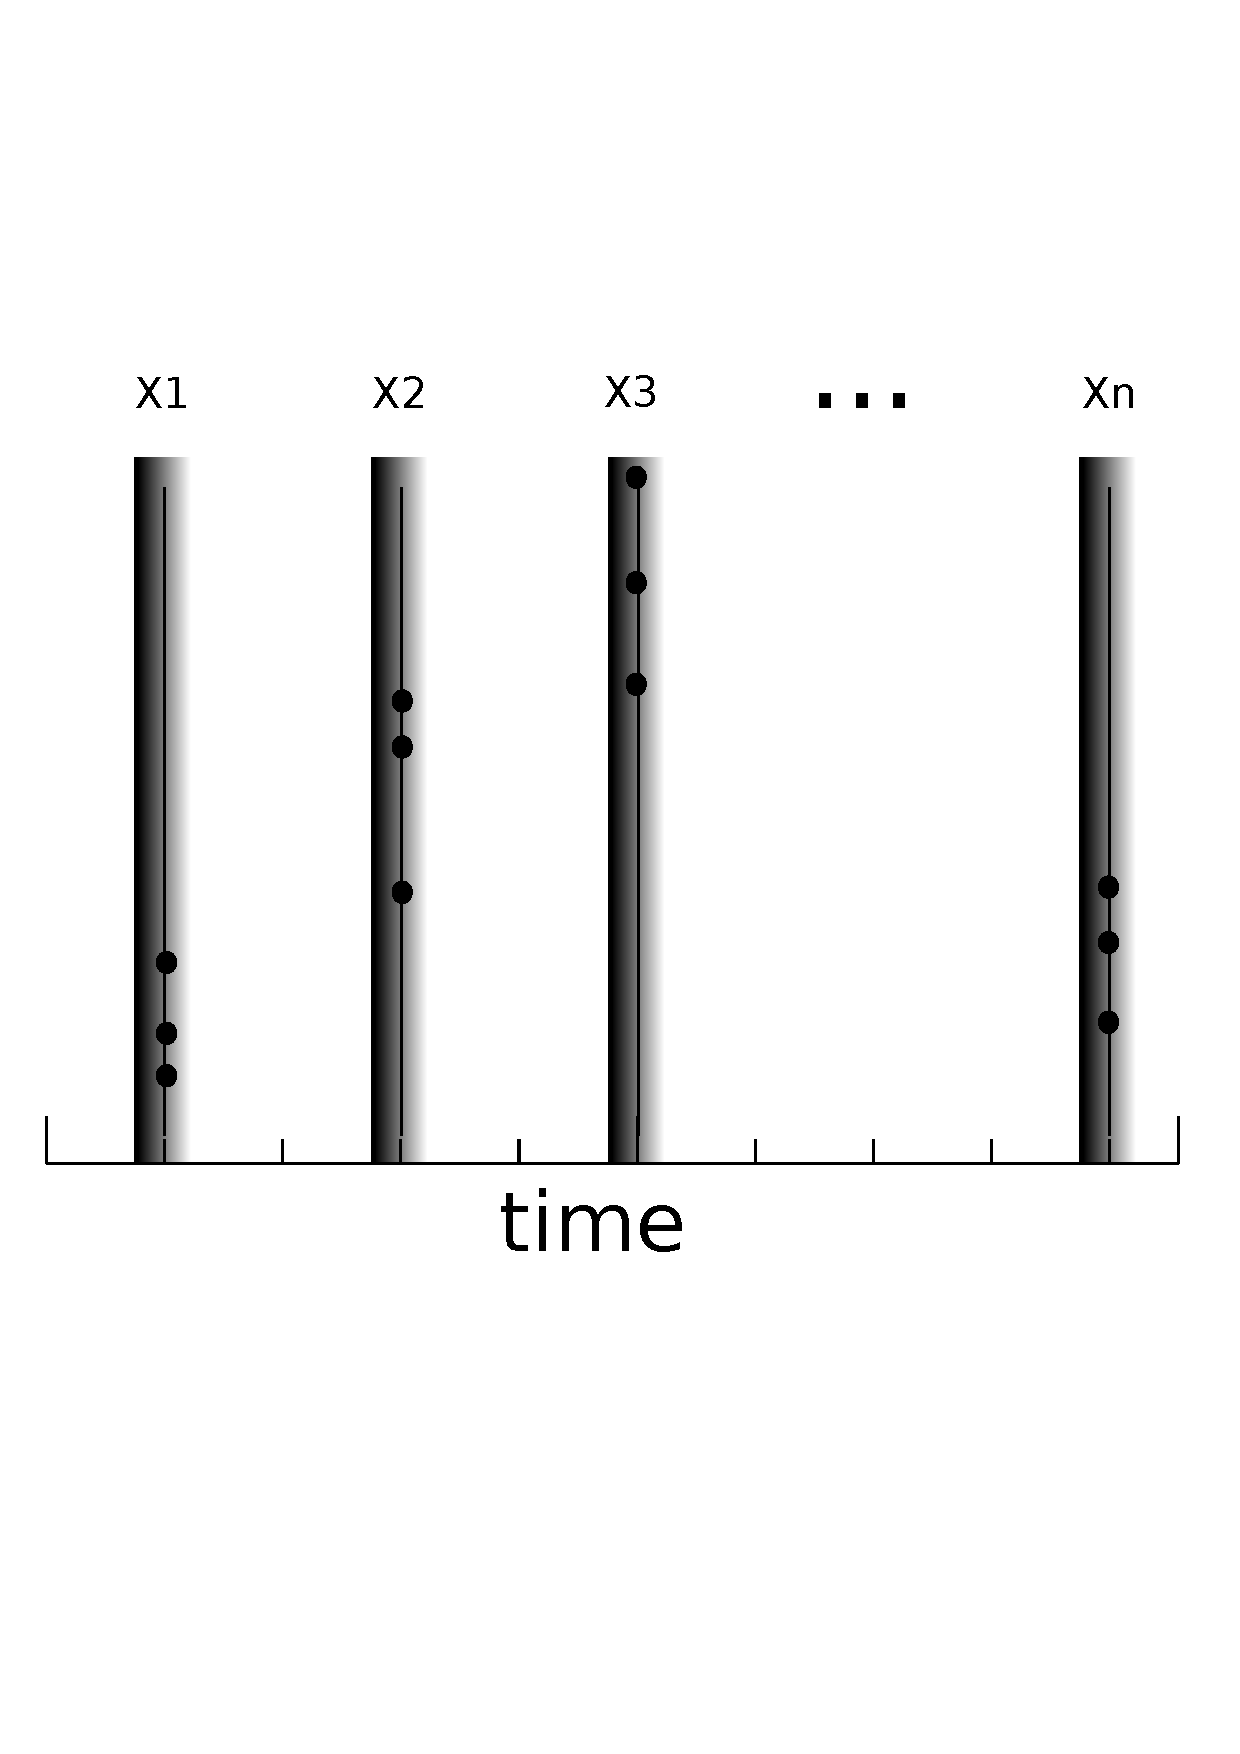
\includegraphics[scale=0.4]{images/multiset2}
    \caption{Multiset-based model of uncertain time series}
  \label{multiset}
  \end{figure}

\paragraph{} In \textbf{PDF-based model}, each element $X_i, (1\leq i \leq n)$ of UTS $X = <X_1, \ldots, X_n>$ is   represented as a random variable $X_i=x_i + X_{e_i}$, where $x_i$ is the exact value that is   unknown and $X_{e_i}$ is a random variable representing the error (Fig. \ref{pdf}). It is this model that we  consider this work.
  
  \begin{figure}
  \centering
   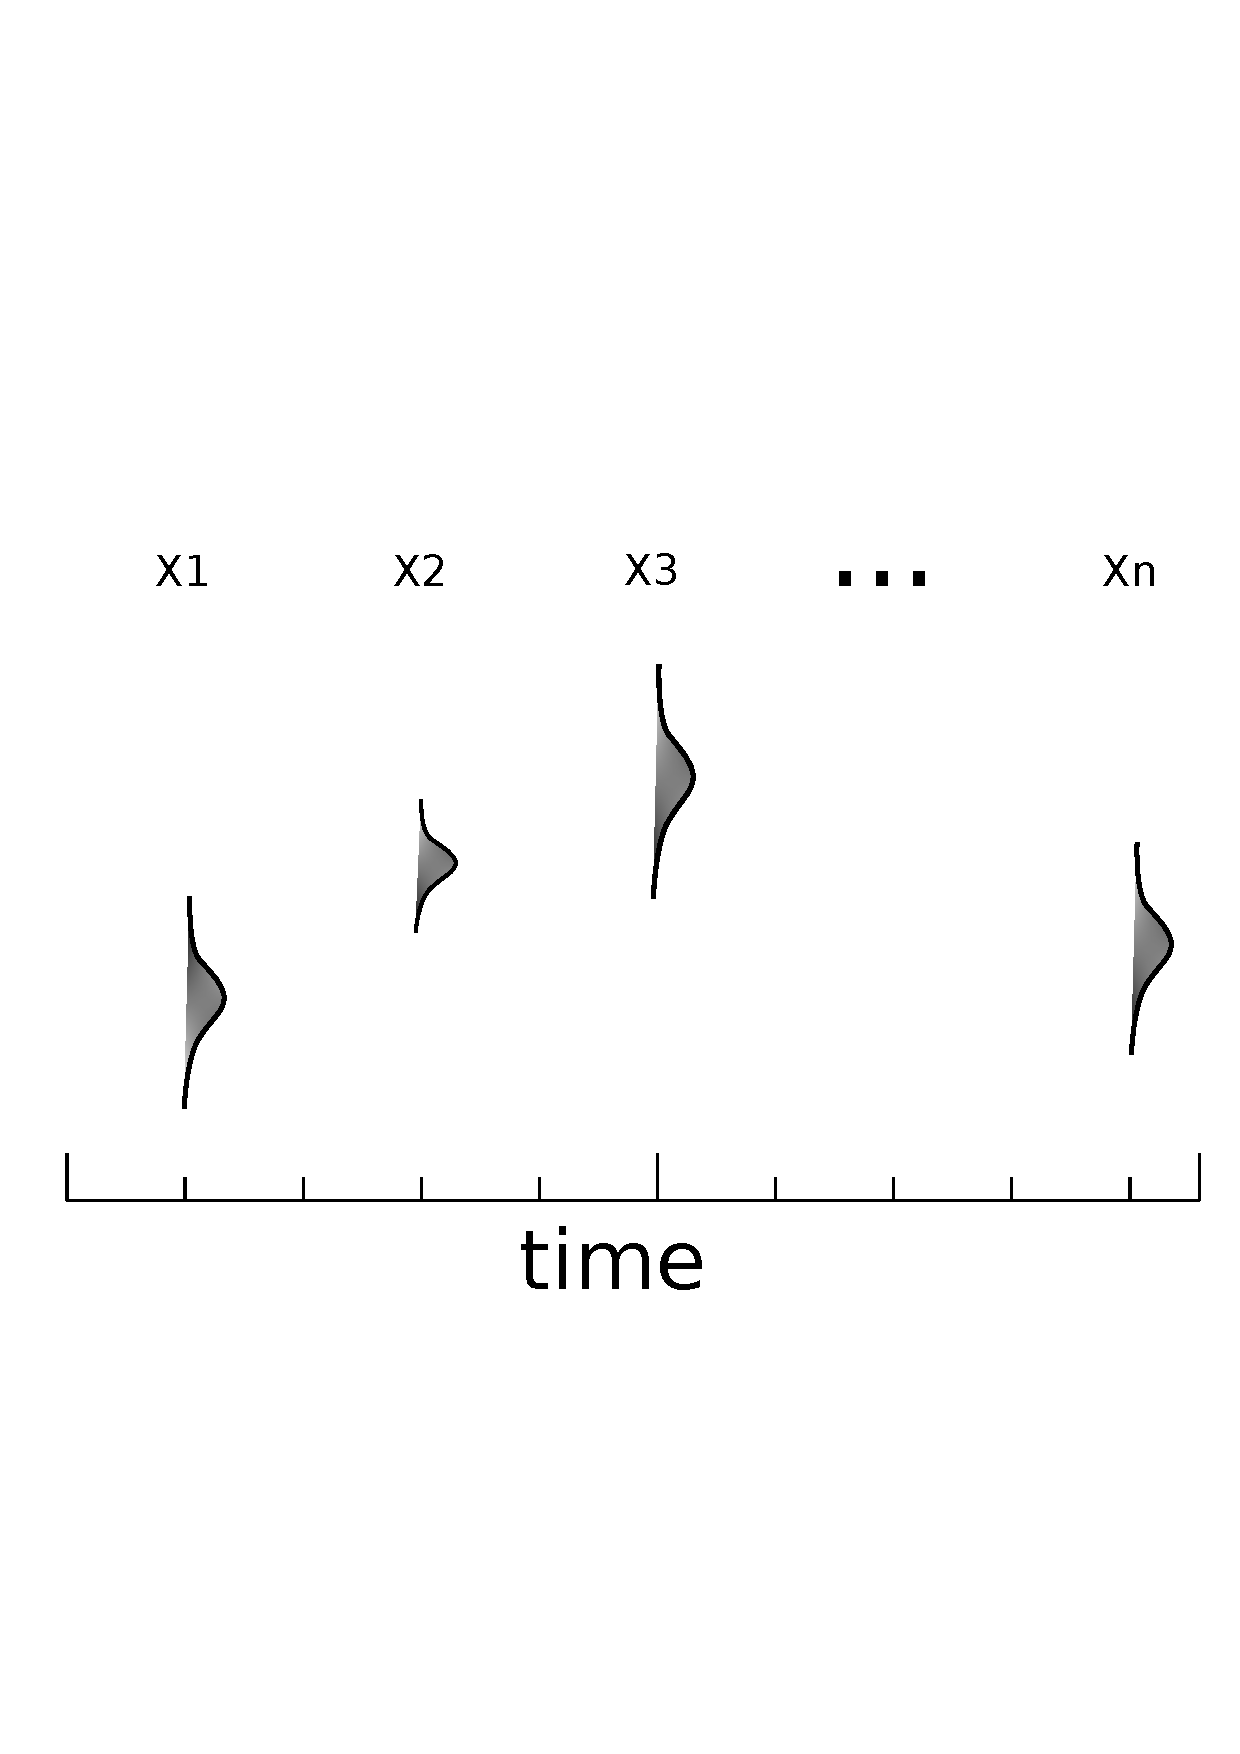
\includegraphics[scale=0.4]{images/pdf2}
  \caption{PDF-based model of uncertain time series}
  \label{pdf}
  \end{figure}
  


Several similarity measures have been proposed for uncertain time series. They are grouped into two main categories: Traditional similarity measures and uncertain similarity measures.

\begin{itemize}
  \item Traditional similarity measures such as Euclidean distance are those conventionally used with time series. They use a single uncertain value at each timestamp as an approximation of
  the unknown real value.
  \item Uncertain similarity measures use additional statistical information that quantifies the uncertainty associated with each approximation of the real value : this is the case of
  DUST, PROUD, MUNICH\cite{dallachiesa}. \cite{Orang2015} demonstrates that the performances of Uncertain similarity measures associated with pre-processing of data are higher than those of traditional similarity measurements.
\end{itemize}


\subsection{Review of u-shapelets}

\begin{definition}
Two datasets  $D_A$ and $D_B$ are said to be \textbf{r-balanced} if only if
$\frac{1}{r}<\frac{|D_{A}|}{|D_{B}|}<(1-\frac{1}{r}),\,r>1$
\end{definition}


\begin{definition}
An \textbf{Unsupervised-Shapelet} is any sub-sequence that has a length shorter than or equal to the length of the shortest time series in the dataset, and that allows dividing the dataset into two
\textbf{r-balanced} groups $D_A$ and $D_B$; where $D_A$ is the group of time series that contains a pattern \textbf{similar} to the shapelet and $D_B$ is the group of
time series that does not contain the shapelet.
\end{definition}

The similarity between a time series and a shapelet is evaluated using a distance function.


\begin{definition}
The sub-sequence distance \textbf{sdist(S, T)} between
a time series T and a sub-sequence S is the minimum of the
distances between the sub-sequence S and all possible
sub-sequences of T of length equal to the length of S.
\end{definition}
This definition opens the question of which distance measure to use for $sdist$.
In general, the ubiquitous Euclidean distance (ED) is used, but it is not
appropriate for uncertain time series \cite{Orang2014}. In the following section, we introduce a
dissimilarity function that is more adapted to  uncertainty.   


Computing the $sdist$ between a u-shapelet candidate
and all time series in a dataset creates an orderline:


\begin{definition}
An orderline is a vector of sub-sequence
distances sdist(S, Ti) between a u-shapelet and all time series Ti in the dataset.
\end{definition}

The computation of the orderline is time-consuming. An orderline for a single u-shapelet candidate is $O(NMlog(M))$ where N is the number of time series in the dataset and M is the average length of the time series. The brute force algorithm for U-shapelets discovery requires K such computations, where K is the number of sub-sequences. The strategy used by \cite{ulanova2015scalable} in \textbf{Scalable Unsupervised Shapelet algorithm} consists in filtering the K candidate segments  by considering only those allowing to build r-balanced groups.  This selection is made efficiently thanks to a hash algorithm.       


The assessment of a u-shapelet quality is based on its separation power which is calculated as follows :
\begin{eqnarray}
gap=\mu_{B}-\sigma_{B}-(\mu_{A}-\sigma_{A}),
\end{eqnarray}


where $\mu_{A}$ (resp. $\mu_{B}$) denotes mean(sdist(S, $D_A$)) (resp. mean(sdist(S, $D_B$))), and
$\sigma_{A}$ (resp. $\sigma_{B}$) represents standard deviation of $sdist(S,
D_A)$ (resp. standard deviation of $sdist(S, D_B)$).
If $D_A$ or $D_B$ consists of only one element (or of an insignificant number of elements that cannot represent a separate cluster), the gap score is assigned to zero. This ensures that a  high gap scored for a u-shapelet candidate corresponds to a true separation power.   

\subsection{Review on uncertain similarity functions}


Uncertain similarity measures  can be grouped into two broad categories : deterministic similarity measurements and probabilistic similarity measurements.

\subsubsection{Deterministic Similarity Measures} 
Like traditional similarity measures, deterministic  similarity measures  return a real number as the distance between two uncertain time series. \textbf{DUST} is an example of deterministic similarity measure.
\paragraph{DUST}
\cite{murthy2013generalized} Given two uncertain time series $X=<X_1, \ldots,X_n>$ and $Y=<Y_1, \ldots,Y_n>$ , the distance between two uncertain values $X_i$, $Y_i$ is defined as the distance between their true (unknown) values r($X_i$), r($Y_i$): $dist(X_i, Y_i) = |r(X_i) - r(Y_i)|$. This distance is used to measures the similarity of two uncertain values. 

$\varphi(|X_{i}-Y_{i}|)$ is the probability that the real values at timestamp i are equal, given the observed values at that instant :
\begin{eqnarray}
\varphi(|X_{i}-Y_{i}|)=Pr(dist(0, |X_{i}-Y_{i}|)=0).
\end{eqnarray}
This similarity function is then used inside the $dust$ dissimilarity function:
\begin{eqnarray}
dust(X_{i},Y_{i})=\sqrt{-log(\varphi(|X_{i}-Y_{i}|))+log(\varphi(0))}.
\end{eqnarray}
The distance between uncertain time series $X=<X_1, \ldots,X_n>$ and $Y=<Y_1, \ldots,Y_n>$ in $DUST$
is then defined as follows:
\begin{eqnarray}
DUST(X,Y)=\sqrt{\stackrel[i=1]{n}{\sum}dust(X_{i},Y_{i})^{^{2}}}.
\end{eqnarray} 

The problem with the deterministic uncertain distances like $DUST$ is that their expression varies as a function of the probability distribution of uncertainty,  and the probability distribution of the uncertainty is not always available in time series datasets.


\subsubsection{Probabilistic Similarity Measures}
Probabilistic similarities measures do not require knowledge of the uncertainty probability distribution. Furthermore, they provide the users with more information about the reliability of the result. There are several probabilistic similarity functions, as MUNICH, PROUD, PROUDS or Local Correlation. 
\paragraph{MUNICH}
\cite{assfalg2009probabilistic}
This distance function is suitable for uncertain time series represented by the multiset based model. The probability that the distance between two uncertain time series X and Y is less than a threshold $\varepsilon$ is equal to the number of distances between X and Y, which are less than $\varepsilon$, over the possible number of distances:

\begin{eqnarray}
Pr(distance(X,Y))\leq\varepsilon=\frac{|\{d\in
dists(X,Y)|d\leq\varepsilon\}|}{|dists(X,Y)|}
\end{eqnarray}

The computation of this distance function is very time-consuming.

\paragraph{PROUD}
\cite{yeh2009proud} Let$X=<X_{1},...,X_{n}>$ and $Y=<Y_{1},...,Y_{n}>$ be two
UTS each modeled  by a sequence of random variables, the PROUD distance between X and Y is $d(X,Y)=\stackrel[i=1]{n}{\sum}(X_{i}-Y_{i})^{2}.$
According to the central limit theorem \cite{hoffmann1976law}, the cumulative distribution of the distances approaches asymptotically a normal distribution:

\begin{eqnarray}
d(X,Y)\propto
N(\underset{i}{\sum}E[(X_{i}-Y_{i})^{2}],\underset{i}{\sum}Var[(X_{i}-Y_{i})^{2}])
\end{eqnarray}

As a consequence of that feature of PROUD distance,  the table of the normal centered reduced law can be used to compute the probability that the normalized distance is lower than a threshold:
\begin{eqnarray}
Pr(d(X,Y)_{norm}\leq\epsilon).
\end{eqnarray} 

A major disadvantage of PROUD is its inadequacy for comparing time series of small lengths like u-shapelets. Indeed, the calculation of the probability that the PROUD distance is less than a value is based on the assumption that it follows \textbf{asymptotically} a normal distribution.  Thus, this probability will be all the more accurate as the compared time series are long (more than 30 data points).


\paragraph{PROUDS}\cite{Orang2015} is an enhanced version of PROUD, which suppose that random variables coming from time series are independent and
identically distributed. 


\begin{definition}
\label{normal}
The normal form of a standard time series $X = <X_1, \ldots, X_n>$ is defined as
$\hat{X}=<\hat{X_{1}},\ldots,\hat{X_{n}}>$ in which for each timestamp i $(1 \leq i \leq n)$, we have:

\begin{eqnarray}
\hat{X_{i}}=\frac{X_{i}-\bar{X}}{S_{X}},\:\bar{X}=\stackrel[i=1]{n}{\sum}\frac{X_{i}}{n},\:S_{X}=\sqrt{\stackrel[i=1]{n}{\sum}\frac{(X_{i}-\bar{X})^{^{2}}}{(n-1)}}.
\end{eqnarray}
\label{normal}
\end{definition}



PROUDS defines the distance between two normalized time series  $\hat{X}=<\hat{X}_{1}...\hat{X}_{n}>$ and $\hat{Y}=<\hat{Y}_{1}...\hat{Y}_{n}>$ (Definition \ref{normal}) as follows:

\begin{eqnarray}
Eucl(\hat{X},\hat{Y})=2(n-1)+2\stackrel[i=1]{n}{\sum}\hat{X}_{i}\hat{Y}_{i}
\end{eqnarray}

For the same reasons as PROUD, PROUDS is not suitable for short time series comparison. Another disadvantage of PROUDS is that it assumes that the random variables  are independent : this hypothesis is strong and particularly inappropriate for short time series like u-shapelets. A more realistic hypothesis with time series would be to consider that the random variables constituting the time series are M-dependent. Random variables of a time series are called M-dependent
 if $X_{i},X_{i+1},...,X_{i+M}$ are dependent (correlated) and the
variables $X_{i}$ and $X_{i+M+1}$ are independent. However, the M-dependent assumption could make PROUDS writing more complex and its use more difficult because of the choice of the parameter M. 


\paragraph{Uncertain Correlation} \cite{Orang2017} : 
Correlation analysis techniques are useful for feature selection in uncertain time series data. Indeed, correlation indicates the degree of dependency of a feature on other features. Using this information, redundant features can be identified. The same strategy can be useful for  u-shapelet discovery.  Uncertain
correlation is defined as follows : 


\begin{definition}
(Uncertain time series correlation) Given UTS  $X = <X_1, \ldots, X_n>$ and  $Y = <Y_1, \ldots, Y_n>$, their correlation is defined as:
\begin{eqnarray}
Corr(X,Y)=\stackrel[i=1]{n}{\sum}\hat{X_{i}}\hat{Y_{i}}/(n-1),
\end{eqnarray}
where $\hat{X_{i}}$ and
$\hat{Y_{i}}$ are normal forms of $X_i$ and $Y_i$ (Definition \ref{normal}), respectively. $X_i$ and $Y_i$ are supposed to be independant continous random variables.
\end{definition}
If we know the probability distribution of random variables, it is possible to determine the probability density function associated with the correlation, which will subsequently be used to calculate the probability that the correlation between two time series is greater than a given threshold.   
Uncertain correlation has however some drawbacks :
\begin{itemize}
\item It is too sensitive to transient changes, often leading to widely fluctuating scores;
\item It cannot capture complex relationship in timeseries;
\item It requires to know the probability distribution function of the uncertainty or to make some assumption on the independence of the random variables  contained in time series.

\end{itemize}
Because of all thoses drawbacks, uncertain correlation cannot be used as it is for u-shapelet discovery. The next paragraph presents a generalisation of correlation coefficient that is not an uncertain similarity function but is still interesting for u-shapelet discovery.

\paragraph{Local Correlation} \cite{papadimitriou2007time} is a
generalization of the correlation. It computes a time-evolving correlation scores that tracks a local similarity on multivariate time series based on local autocorrelation matrix. The autocorrelation matrix \textbf{allows capturing complex relationship} in time series like the key oscillatory (e.g., sinusoidal) as well as aperiodic trends (e.g., increasing or decreasing)  that are present. The use of  autocorrelation
matrices which are computed based on overlapping windows allows \textbf{reducing the sensibility to transient changes} in time series.


\begin{definition}
(Local autocovariance, sliding window). Given a time series $X$, a sample set of windows with length w, the local autocorrelation matrix estimator $\hat{\Gamma}_{t}$ using a sliding window is defined at time $t \in \mathbb{N} $ as (Eq.\ref{autoCor}) : 

\begin{eqnarray}
\hat{\varGamma}_{t}(X,w,m)=\stackrel[\tau=t-m+1]{t}{\sum}x_{\tau,w}\otimes x_{\tau,w}.
\label{autoCor}
\end{eqnarray}

where $\boldsymbol{x}_{\tau,\omega}$ is a sub-sequence of the time series of length $w$ and started at $\tau$, $x \otimes y = xy^T$ is the outer product of x and y. The sample set of m windows is centered around time t.
We typically fix the number of windows to m = w.
\end{definition}

Given the estimates $\hat{\Gamma}_{t}(X)$ and $\hat{\Gamma}_{t}(Y)$ for the two time series, the next step is how to compare them and extract a correlation score. This goal is reached using the spectral decomposition; The eigenvectors of the autocorrelations matrices capture the key aperiodic and oscillatory trends, even \textbf{in short time series}.  Thus, the subspaces spanned by the first few (k) eigenvectors are used  to locally characterize the behavior of each series. Definition \ref{score} formalizes this notion: 


\begin{definition}
\label{score}
(LoCo score). Given two series $X$ and $Y$, their LoCo score is defined by

\begin{eqnarray}
\ell_{t}(X,Y)=\frac{1}{2}(\Vert
\boldsymbol{U}_{X}^{T}\boldsymbol{u}_{Y}\Vert+\Vert
\boldsymbol{U}_{Y}^{T}\boldsymbol{u}_{X}\Vert)
\end{eqnarray}

\end{definition}    
   

Where $\boldsymbol{U}_X$ and  $\boldsymbol{U}_Y$ are the k first eigenvector
matrices of the local autocorrelation $\hat{\Gamma}_{t}(X)$ and
$\hat{\Gamma}_{t}(Y)$ respectively, and $u_X$  and $u_Y$  are the
corresponding eigenvectors with the largest eigenvalue. 

\begin{figure}
\centering
 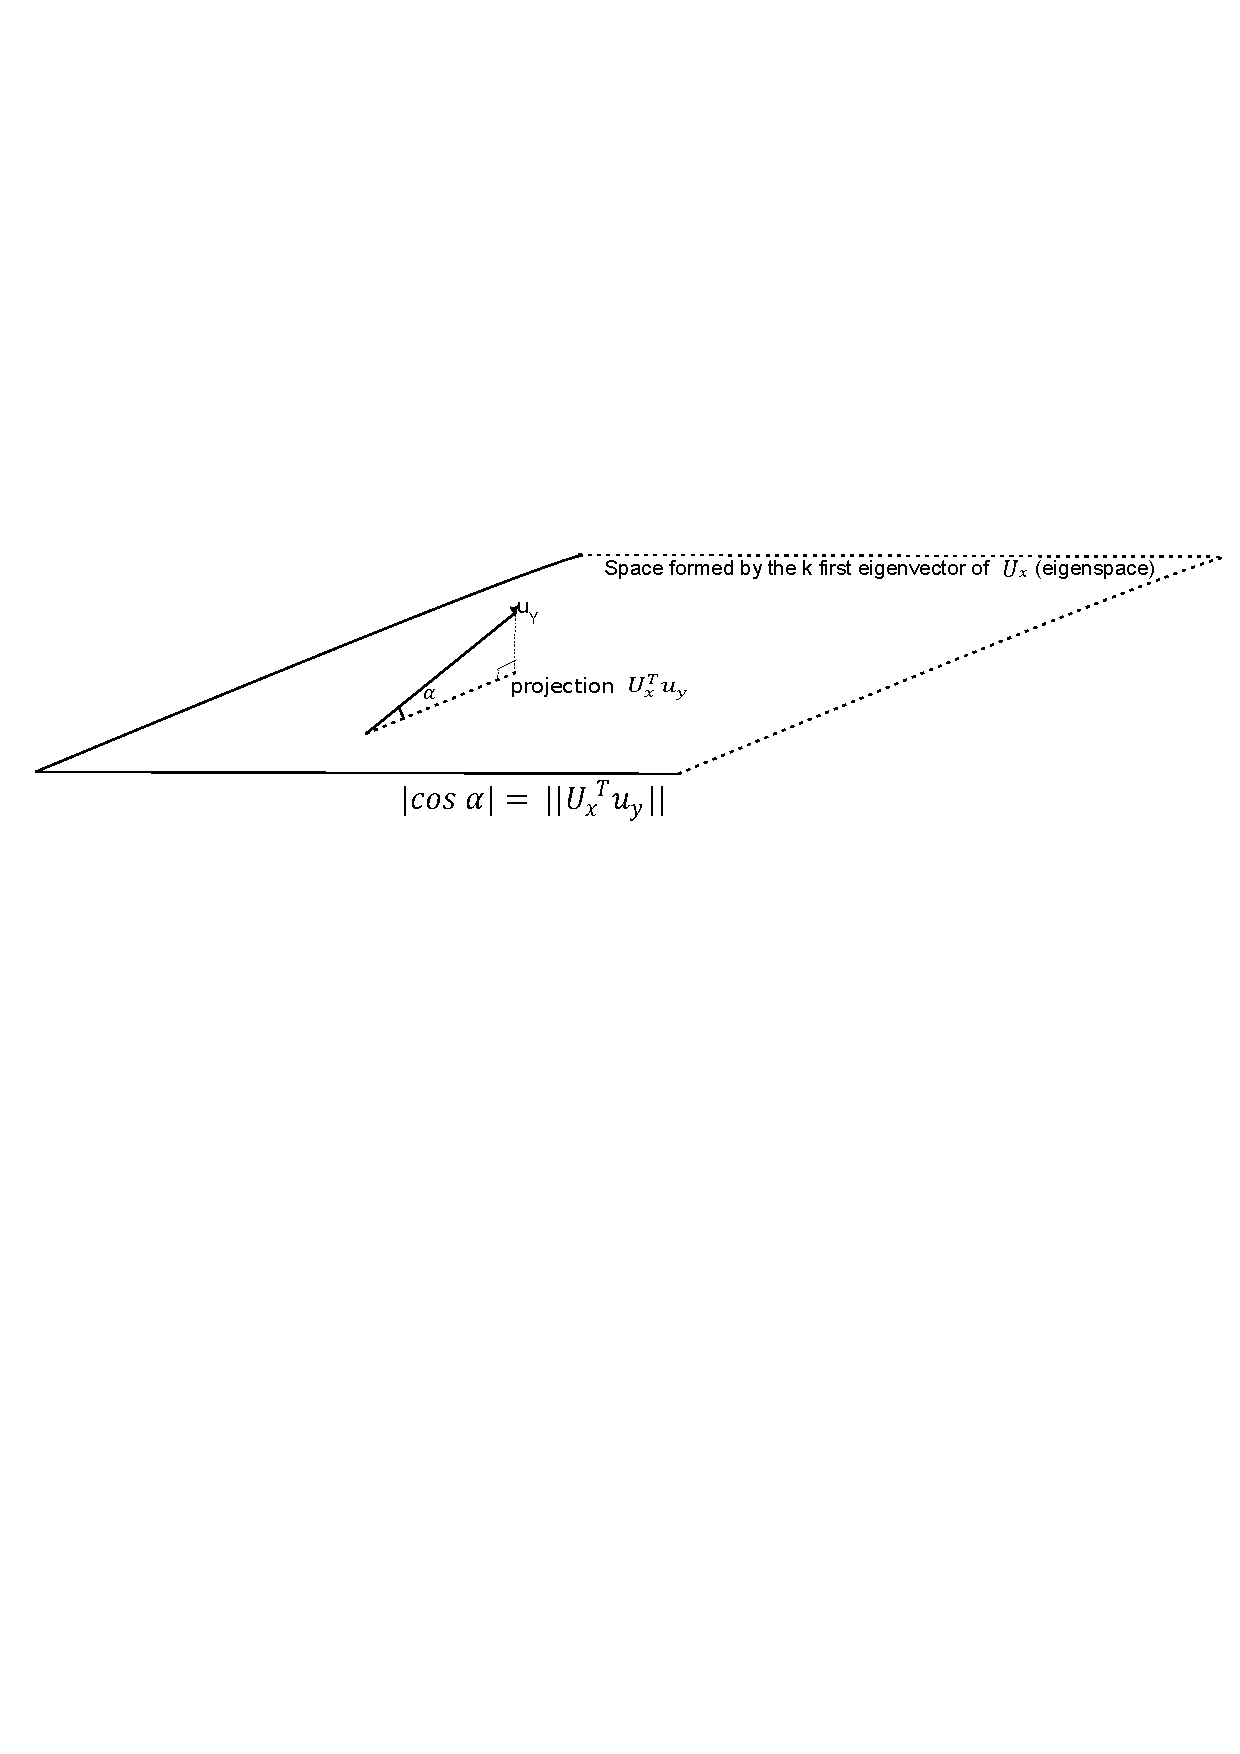
\includegraphics[scale=0.70]{images/loco2}
\caption{Geometric representation of loco similarity.}
\label{geoLoco}
\end{figure}


Intuitively, two time series X and Y will be considered as close when the angle
$\alpha$ formed by the space carrying the information of the time series X and
the vector carrying the information the time series Y is zero. In other words X
and Y will be close when the value of the $cos(\alpha)$ will be 1. The only
assumption made for the computation of LoCo similarity is that the mean of time
series data point is zero. This could be easily achieve with z-normalization.
LoCo similarity function has many interesting properties and does not require to:
\begin{itemize}
  \item Know the probability distribution of the uncertainty,
  \item Assume the independence of the random variables or the length of
  u-shapelets.
\end{itemize}

It is therefore interesting for feature selection, but we still need a dissimilarity
function to be able to discover u-shapelet. In the next paragraph, we 
define a dissimilarity function that has the same properties as LoCo and that is
robust to the presence of uncertainty.
\section{Our Approach}
\subsection{Dissimilarity function}

The LoCo similarity function defined on two multivariate time series X and Y approximately corresponds  to the absolute value of the cosine of the angle formed by the eigenspaces of X and Y ($|cos(\alpha)|$). A straightforward idea would be to use the $sin(\alpha)$ or $\alpha$-value as a dissimilarity function but this approach does not work so well; the sine and the angle are not discriminant enough for eigenvector comparison for clustering purpose. We thus propose the following dissimilarity measure (Definition. \ref{FOTS}). 


\begin{definition}
\label{FOTS}
(FOTS : Frobenius cOrrelation for uncertain Time series uShapelet discovery) Given two series $X$
and $Y$, their FOTS score is defined by
\begin{eqnarray}
FOTS(X,Y)=\Vert U_{X}-U_{Y}\Vert_{F}
=\sqrt{\stackrel[i=1]{m}{\sum}\stackrel[j=1]{k}{\sum}(U_{X}-U_{Y})_{ij}^{2}}
\end{eqnarray}
where $\Vert\Vert_{F}$ is the Frobenius norm.
\end{definition}
 
 Because the FOTS computation is based on the comparison of the k-first eigenvectors of the autocorrelation
 matrices of the time series, it has the same desirable properties of the LoCo
 similarity function, that is: 
 
 \begin{itemize}
   \item It \textbf{allows to capture complex relationship}
in time series like the key oscillatory (e.g., sinusoidal) as well as aperiodic (e.g.,
increasing or decreasing) trends that are present;
   \item It allows to \textbf{reduce the sensibility to transient changes} in time
   series;
   \item It is appropriate for the \textbf{comparison of short
   timeseries}.
 \end{itemize}

  Moreover, the FOTS dissimilarity function is \textbf{robust to the presence of
  uncertainty} due to the spectral decomposition of the autocorrelation matrices of the time series. The robustness of FOTS to the uncertainty is confirmed by the following theorem:   

\begin{theorem}
\textbf{(Hoffman\-Wielandt)} \cite{Bhatia1993} If $X$ and $X + E$ are $n \times
n$ symmetric matrices, then : 
\begin{eqnarray}
\stackrel[i=1]{n}{\sum}(\lambda_{i}(X+E)-\lambda_{i}(X))^{2}\leq||E||_{F}^{2}.
\end{eqnarray}
where $\lambda_i(X)$ is the ith largest eigenvalue of $X$, and $||E||_{F}^{2}$
is the squared of the Frobenius norm of E.
\end{theorem}

The next section explains how FOTS is integrated in the Scalable Unsupervised Shapelet discovery algorithm.


\subsection{Scalable u-shapelets Algorithm with FOTS score}
In this section we do not define a new SUShapelet algorithm, but we explain how we use SUShapelet algorithm with FOTS score (FOTS-SUSh) to deal with uncertainty.


 Two main criteria make  possible to evaluate the quality of a u-shapelet:
\begin{itemize}
  \item It has to produce two r-balanced groups.
  \item It must build two well separated groups, i.e., groups whose gap is
  maximal.
\end{itemize}

The gap is, therefore, an essential criterion for the selection of u-shapelets candidate. It is subject to uncertainty because its calculation is based on the
Euclidean distance. To remedy this, we propose to use the FOTS score instead of
a simple Euclidean distance when calculating the gap in the Scalable u-shapelet algorithm. Algorithms \ref{algo1} and \ref{algo2} present a more formal definition:    


 \begin{definition}
The sub-sequence FOTS dissimilarity $\boldsymbol{sd_f(S, T)}$ between
a time series T and a sub-sequence S is the minimum of the FOTS
score between the sub-sequence S and all possible
sub-sequences of T of length equal to the length of S.
\end{definition}


\begin{algorithm}[h]
\DontPrintSemicolon
\KwIn{u-shapeletCandidate : s,\\ time series dataset : D}
\KwOut{Distance between the u-shapelet Candidate and all the time series of the
dataset}
\SetKwBlock{Begin}{function}{end function}

\Begin($\text{ComputeOrderline} {(} s, \, D{)}$)
{
  $dis \leftarrow \{\}$\;
  $s \leftarrow zNorm(s)$\;
  \ForAll{$i \in \left\lbrace  1, 2, \ldots, |D|\right\rbrace$}
  {
    $ts \leftarrow D(i,:)$\;
    $dis(i) \leftarrow sd_f(s,ts)$\;    
  }  
  \Return{$\nicefrac{dis}{|s|}$}

}
\caption{ComputeOrderline}
\label{algo1}
\end{algorithm}



\begin{algorithm}[h]
\DontPrintSemicolon
\KwIn{u-shapeletCandidate : s,\\ 
timeseries dataset : D, \\
lb, ub : lower/upper bound of reasonable number of time series in cluster}
\KwOut{gap : gap score}
\SetKwBlock{Begin}{function}{end function}

\Begin($\text{ComputeGap} {(} s, \, D, \, lb, \, ub{)}$)
{
  $dis \leftarrow ComputeOrderline(s,D)$\;
  $gap \leftarrow 0$\;
  
     \For{$i \leftarrow lb \, \boldsymbol{to} \, ub$}
    {
        $D_A \leftarrow dis \leq dis(i)$,
        $D_B \leftarrow dis > dis(i)$
        
      \uIf{$lb \leq |D_A| \leq ub$}
      {
       $m_A \leftarrow mean(D_A) $,
       $ m_B \leftarrow mean(D_B)$\;
       
       $s_A \leftarrow std(D_A)$,
       $s_B \leftarrow std(D_B)$\;
       
       $currGap \leftarrow m_B - s_B - (m_A + s_A)$
       
       \uIf{$currGap > gap$}
       {
       	$gap \leftarrow currGap$
       } 
      }
    }  
  \Return{$gap$}

}
\caption{ComputeGap}
\label{algo2}
\end{algorithm}

\section{Experimental Evaluation}

\subsection{Clustering with u-shapelets}
The algorithm iteratively splits the data with each discovered u-shapelet: each u-shapelet splits the dataset into two groups $D_A$ and $D_B$. The time series that belong to $D_A$ are considered as members of the cluster form by the u-shapelet and are then removed from the dataset. A new u-shapelet search continues with the rest of the data until there is no more time series in the dataset or until the algorithm is no more able to find u-shapelet. As a stopping
criterion for the number of u-shapelets extracted, the decline of the u-shapelet gap score is
examined: the algorithm stops when the gap score of the newly-found u-shapelet
becomes less than half of the gap score of the first discovered u- shapelet. This approach is a direct implementation of the u-shapelet definition

\paragraph{Choosing the length $N$ of a uShapelet : }
The choice of the length of u-shapelet is directed by the knowledge of the
domain to which the time series belongs. As part of these experiments, we tested all  numbers between 4 and half the length of the time series. We consider as length of u-shapelet the one allowing to better cluster the time series.

\paragraph{Choosing the length $w$ of the windows : }
The use of overlapping windows for calculating the autocorrelation matrix makes
it possible to capture the oscillations present in the time series. During these experiments, we consider that the size of the window is equal to half the length of the u-shapelet.
  
\paragraph{Choosing  the number $k$ of eigenvectors: }
A practical choice is to fix $k$ to a small value; we use $k = 4$ throughout all
experiments. Indeed, key aperiodic trends are captured by one eigenvector,
whereas key oscillatory trends manifest themselves in a pair of eigenvectors.  

\subsection{Evaluation Metric}
To appreciate the quality of the u-shapelets found, we use them for a clustering task. The quality of clustering is evaluated from the Rand Index \cite{rand1971objective} which is calculated as follows:

Let Lc be the cluster labels returned by a clustering algorithm and Lt be the
set of ground truth class labels. Let A be the number of time series that are
placed in the same cluster in Lc and Lt, B be the number of time series in
different clusters in Lc and Lt, C be the number of time series in the same
cluster in Lc but not in Lt and D be the number of time series in different
clusters in Lc but in same cluster in Lt. The Rand Index is equals to : 

\begin{eqnarray}
Rand\,Index = (A+B)/(A+B+C+D)
\end{eqnarray}    

\subsection{Comparison with u-shapelet}
Similarly to \cite{dallachiesa}, we tested our method on 17 datasets coming from UCR archive \cite{UCRArchive} representing a wide range of application domains. The training and testing sets have been joined to obtained bigger datasets. Table \ref{datasets} present detailed information about tested datasets.



\begin{table}[ht]
\centering
\small
\begin{tabular}{lcccl}
\textbf{Data-set}   & \textbf{Size of  } & \textbf{Length} & \textbf{No. of  } & \textbf{Type} \\
\textbf{ }   & \textbf{  dataset} & \textbf{ } & \textbf{  Classes} & \textbf{ } \\
50words            & 905                      & 270             & 50                      & IMAGE         \\
Adiac              & 781                      & 176             & 37                      & IMAGE         \\
Beef               & 60                       & 470             & 5                       & SPECTRO       \\
Car                & 120                      & 577             & 4                       & SENSOR        \\
CBF                & 930                      & 128             & 3                       & SIMULATED     \\
Coffee             & 56                       & 286             & 2                       & SPECTRO       \\
ECG200             & 200                      & 96              & 2                       & ECG           \\
FaceFour           & 112                      & 350             & 4                       & IMAGE         \\
FISH               & 350                      & 463             & 7                       & IMAGE         \\
Gun\_Point         & 200                      & 150             & 2                       & MOTION        \\
Lighting2          & 121                      & 637             & 2                       & SENSOR        \\
Lighting7          & 143                      & 319             & 7                       & SENSOR        \\
OliveOil           & 60                       & 570             & 4                       & SPECTRO       \\
OSULeaf            & 442                      & 427             & 6                       & IMAGE         \\
SwedishLeaf        & 1125                     & 128             & 15                      & IMAGE         \\
synthetic\_control & 600                      & 60              & 6                       & SIMULATED     \\
FaceAll            & 2250                     & 131             & 14                      & IMAGE        
\end{tabular}
\caption{Datasets}
\label{datasets}
\end{table}

Table \ref{ri} presents the comparison of the two algorithms.

\begin{table}[ht]
\centering
\begin{tabular}{lcc}
\textbf{Datasets}  & \textbf{RI\_SUSh} & \textbf{RI\_FOTS} \\
50words            & 0.811             & \textbf{0.877}    \\
Adiac              & 0.796             & \textbf{0.905}    \\
Beef               & 0.897             & \textbf{0.910}    \\
Car                & 0.708             & \textbf{0.723}    \\
CBF                & 0.578             & \textbf{0.909}    \\
Coffee             & 0.782             & \textbf{0.896}    \\
ECG200             & 0.717             & \textbf{0.866}    \\
FaceFour           & 0.859             & \textbf{0.910}    \\
FISH               & 0.775             & \textbf{0.899}    \\
Gun\_Point         & 0.710             & \textbf{0.894}    \\
Lighting2          & 0.794             & \textbf{0.911}    \\
Lighting7          & 0.757             & \textbf{0.910}    \\
OliveOil           & 0.714             & \textbf{0.910}    \\
OSULeaf            & 0.847             & \textbf{0.905}    \\
SwedishLeaf        & 0.305             & \textbf{0.909}    \\
synthetic\_control & 0.723             & \textbf{0.899}    \\
FaceAll            & 0.907             & \textbf{0.908}   
\end{tabular}
\caption{Comparison of the Rand Index of SUSH (RI\_SUSh) and FOTS-SUSh (RI\_FOTS). The best Rand Index is in bold}
\label{ri}
\end{table}

				
\subsection{Discussion}

The use of the FOTS score associated with the SUShapelet algorithm makes it
possible to discover different u-shapelets than those found by the Euclidean
distance. The FOTS-SUSh improves the results of time series clustering because the FOTS score takes into account the intrinsic properties of the time series when searching for u-shapelets and is robust to the presence of uncertainty. This improvement is particularly significant when the FOTS score is used for the clustering of time series containing several small oscillations. Indeed, these oscillations are not captured by the Euclidean distance but are by the FOTS score whose calculation is based on the autocorrelation matrix. This observation is illustrated by the result obtained on  SwedishLeaf dataset.

\subsubsection{Time complexity analysis} ED can be computed in $\mathcal{O}(n)$ and  FOTS score is computed in $\mathcal{O}(n^\omega),\:2\leq\omega\leq3$ due to the time complexity of the eigenvector decompositions \cite{pan1999complexity}. The computation of FOTS score is then more expensive than that of ED. However, its use remains relevant for u-shapelet research as they are often small.



\section{Conclusion and Future Work}
The purpose of this work was to discover u-shapelets on uncertain time series. To answer this question, we have proposed a dissimilarity score (FOTS) adapted to the comparison of short time series, whose computation is based on the comparison of the eigenvector of the autocorrelation matrices of the time series. This score is robust to the presence of uncertainty, it is not very sensitive to transient changes, and it allows capturing complex relationships between time series such as oscillations and trends. The FOTS score was used with the Scalable Unsupervised Shapelet Discovery algorithm for clustering 17 literature datasets and showed an improvement in the quality of clustering evaluated using the Rand Index.  By combining the benefits of the u-shapelets algorithm, which reduces the adverse effects of uncertainty, and the benefits of the FOTS score, which is robust to the presence of uncertainty, this work is defining a framework for clustering uncertain time series. As a perspective to this work, we plan to use the FOTS score for fuzzy clustering of uncertain time series.

\chapter[SAX-P]{Symbolic representation of cyclic time series based on properties of cycles}
\label{chapter_saxp}
\begin{abstract} 
The analysis of cyclic time series from bio-mechanics is based on the
comparison of the properties of their cycles. As usual algorithms of time 
series classification ignore this particularity, we propose
a symbolic representation of cyclic time series based on the properties
of cycles, named SAX-P. The resulting character strings can be compared
using the Dynamic Time Warping distance. The application of SAX-P
to propulsive moments of three subjects (S1, S2, S3) moving in Manual
Wheelchair highlight the asymmetry of their propulsion. The symbolic representation 
SAX-P facilitates the reading of
the cyclic time series and the clinical interpretation of the classification results.

\end{abstract} 

\section{Introduction}
\label{introduction}

Generally, during his locomotion, the human being performs cyclic movements (e.g. : walking, running, swimming,
cycling). The bio-mechanical analysis of these movements is performed with various measuring instruments 
(eg force and acceleration sensors, kinematic analysis systems) that enable continuous recording over 
long periods of many kinematic and dynamic parameters. These recordings produce long
time series composed of many cycles or patterns, representative of the movements made and effort 
produced by the subject during his displacement (Fig. \ref{fig:cyclicTS}).


 \begin{figure}[h]
  \centering
   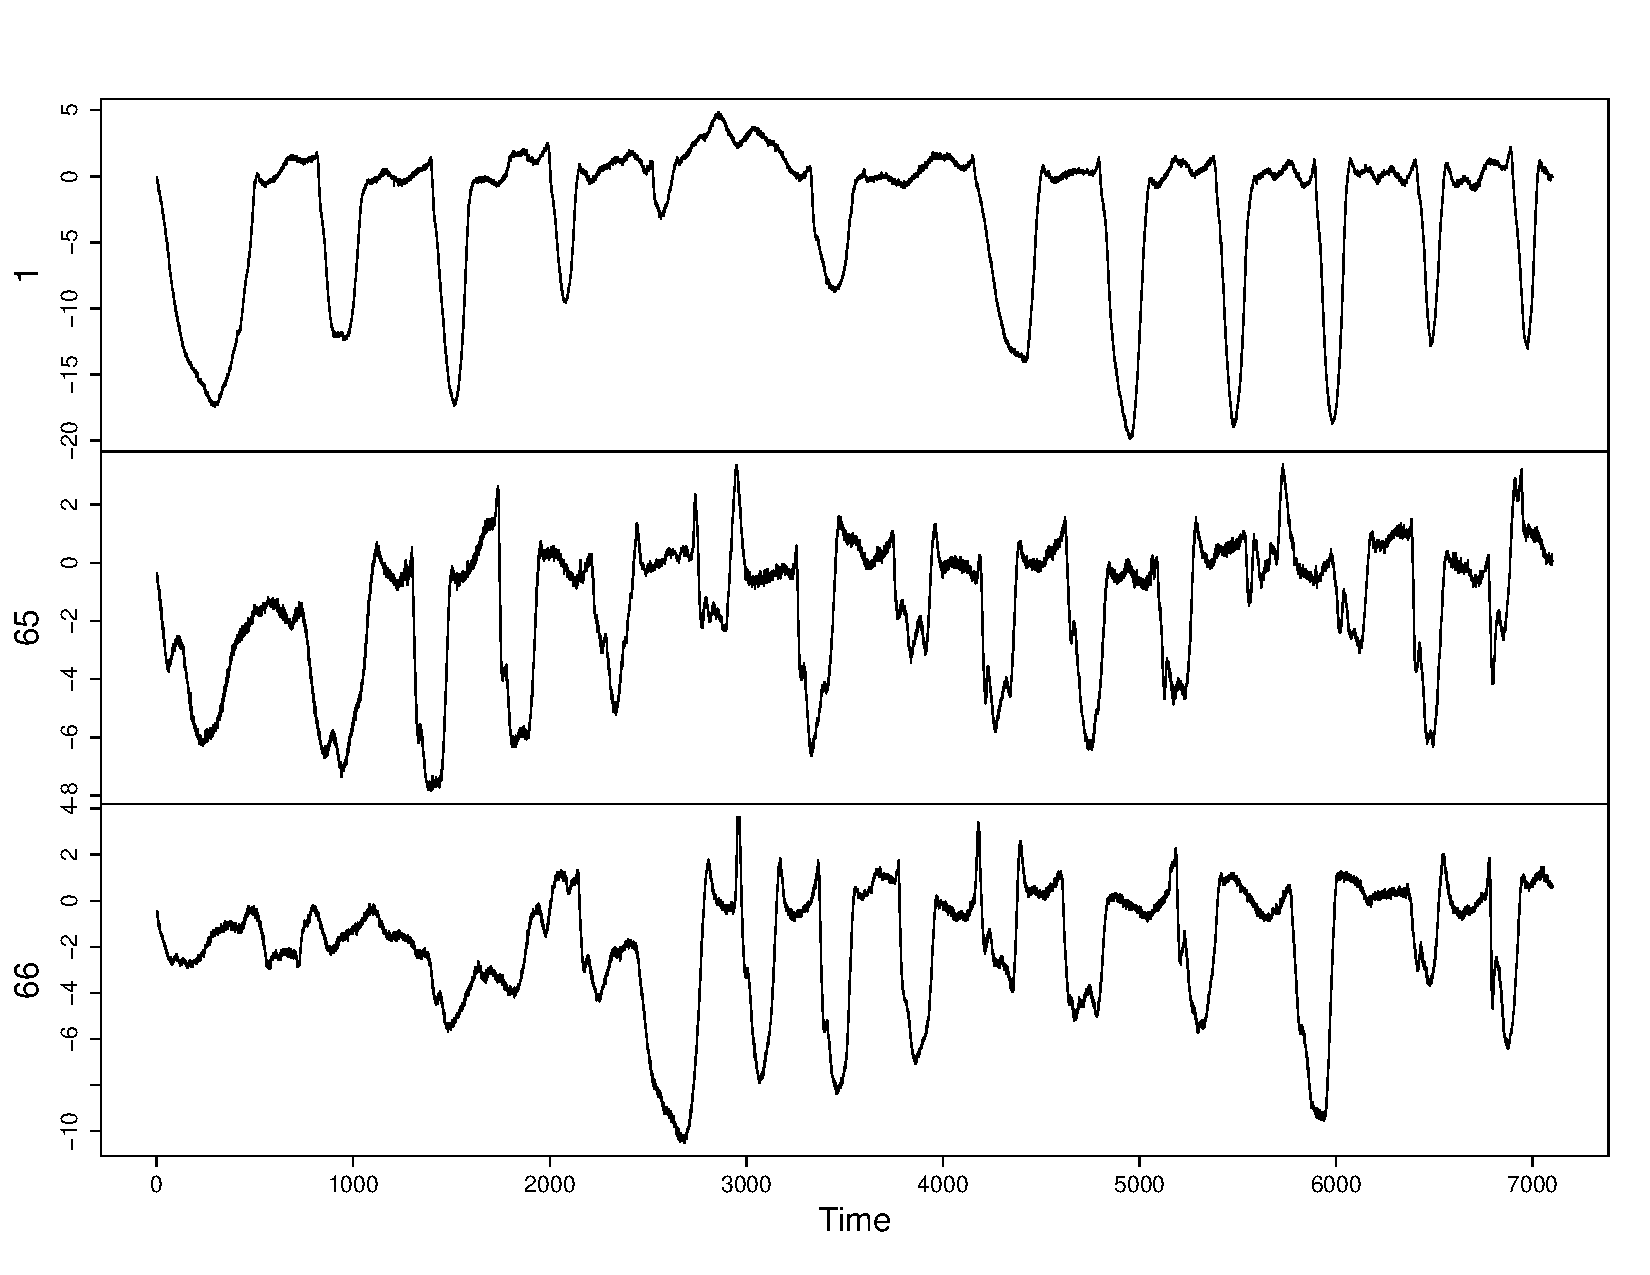
\includegraphics[scale=0.4]{images/sax-p/cycliqueTS}
    \caption{Cyclic time series form manual wheelchair locomotion}
  \label{fig:cyclicTS}
  \end{figure}


These cycles are the time series analysis units and have several
characteristic properties such as the minimum value, the area under the cycle 
\cite{Vegter2014} (Fig. \ref{fig:cycleProp}). 

 \begin{figure}[h]
  \centering
   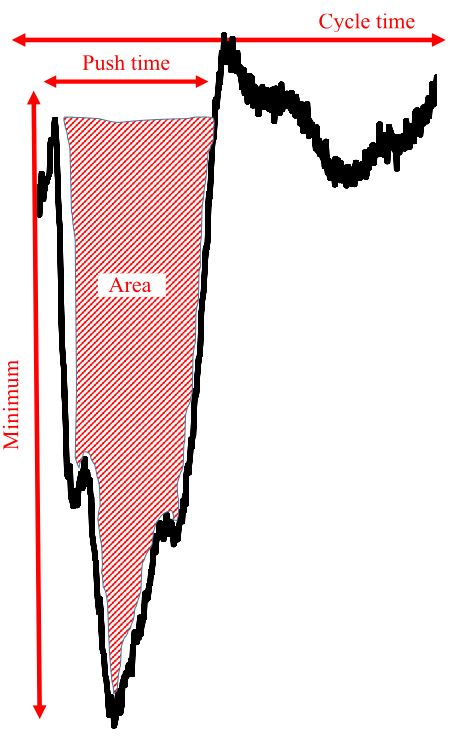
\includegraphics[scale=0.4]{images/sax-p/cycle_prop}
    \caption{Properties of a cycle}
  \label{fig:cycleProp}
  \end{figure}
	

For comparing time series, several previous studies suggested to break them into 
small segments and then to compare the properties of their segments.
A segment of a time series is a sequence of consecutive values belonging to it \cite{Abonyi2003}.


\cite{keogh2001dimensionality} proposed replacing each segment of a time series
$X=x_{1},x_{2},\cdots,x_{n}$ by its mean values;
$\bar{x}_{i}=\frac{N}{n}\sum_{j=\frac{n}{N}(i-1)+1}^{(\frac{n}{N})i}x_{j},$  transforming the time
series, which is a sequence of values, in the suite of the means of its N segments
$\bar{X}=\bar{x}_{1}\bar{,x}_{2},\cdots,\bar{x}_{N}.$ This method is known as Piecewise Aggregate
Approximation (PAA) (Fig. \ref{fig:paa}). The time series $C$ and $Q$ are then compared by calculating the distance $DR$
between the suite $\bar{C}$ and $\bar{Q}$ of the means of their segments :
\begin{equation}
DR(\bar{C},\bar{Q})=\sqrt{\frac{n}{N}\sum_{i=1}^{N}(\bar{c}_{i}-\bar{q}_{i})^{2}}.
\label{equ:paa}
\end{equation}

 \begin{figure}[h]
  \centering
   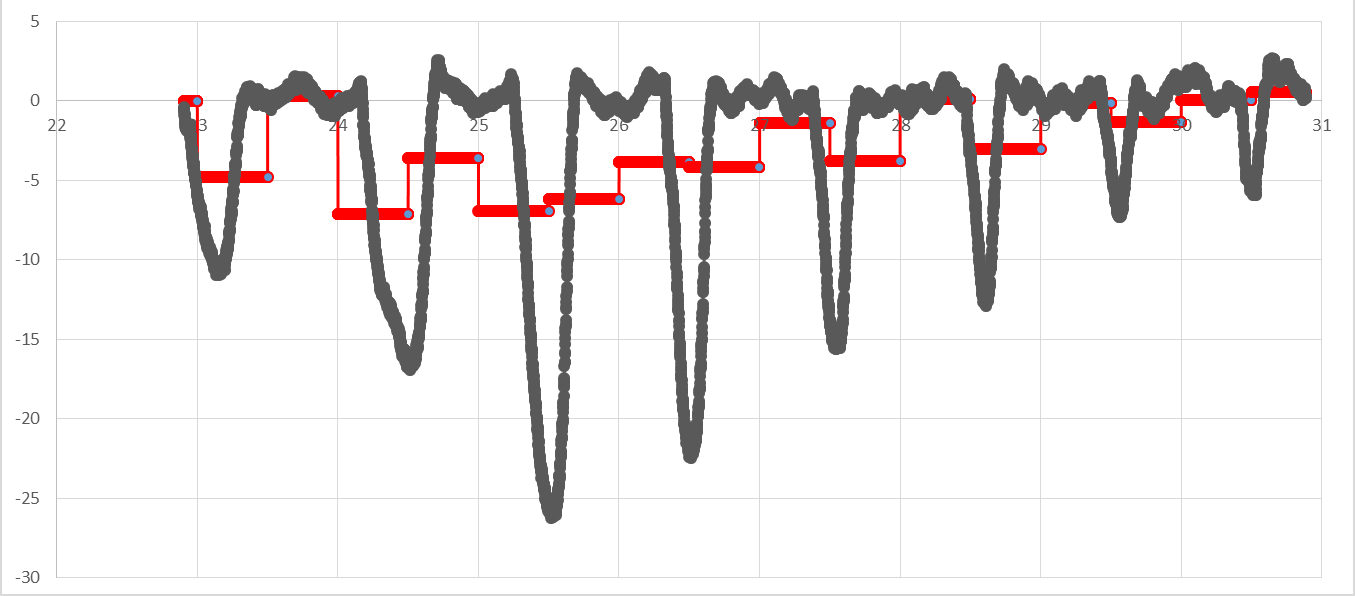
\includegraphics[scale=0.4]{images/sax-p/paa}
    \caption{Piecewise aggregate approximation of a cyclic time series}
  \label{fig:paa}
  \end{figure}

The main objective of PAA was to reduce the length of the time series. However, 
as it computes the segments means, it also allows us to compare two time series C and Q from 
the properties of their 
segments (Equation \ref{equ:paa} ).


\cite{lin2003symbolic} were based on the PAA method to provide a symbolic representation of time
series called Symbolic Aggregate Approximation (SAX). The objective of SAX is to assign a letter to
each segment. To do this, the domain of the values of the time series is divided into intervals
so that every point of the temporal series has approximately the same probability to belong to an 
interval and a letter is associated with each of these intervals.  Then each segment of the time
series is associated with the letter of the interval  to which belongs its average (Fig. \ref{fig:sax}).

 \begin{figure}[h]
  \centering
   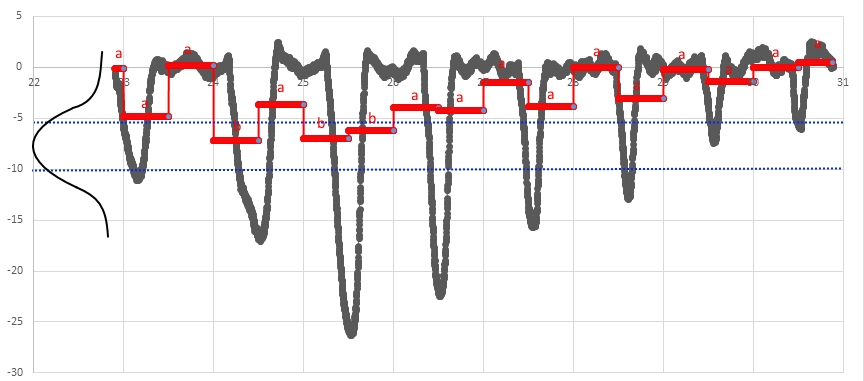
\includegraphics[scale=0.6]{images/sax-p/sax2}
    \caption{Symbolic Aggregate approXimation of a cyclic time series}
  \label{fig:sax}
  \end{figure}
	

With SAX, the distance $MINDIST$ between two strings $\hat{Q}$ and $\hat{C}$ of length $N$ is calculated from the
distance between the borders of the intervals represented by each character in the string 
(Equation \ref{equ:sax}).


\begin{equation}
MINDIST(\hat{Q},\hat{C})=\sqrt{\frac{n}{N}\sum_{i=1}^{N}(dist(\hat{q}_{i},\hat{c}_{i}))^{2}}.
\label{equ:sax}
\end{equation}


$\hat{q}_{i}\:et\:\hat{c}_{i}$ are characters and $ dist() $ is the distance between the borders of 
the intervals which represent these characters  \cite{lin2003symbolic}. However, two segments with very 
different shapes can have the same average and be represented by the same letter: the mean is not 
enough to define a segment. In order to solve this problem, \cite{Lkhagva2006} proposed the ESAX 
model that considers three properties for each segment: its mean, its minimum and maximum (Fig. \ref{fig:esax}).

 \begin{figure}[h]
  \centering
   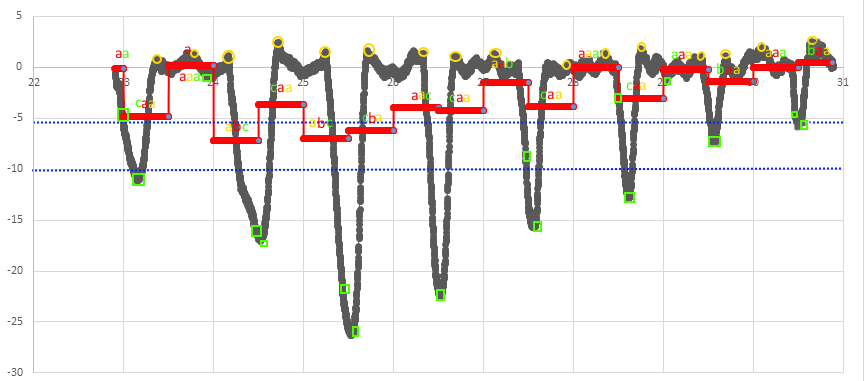
\includegraphics[scale=0.6]{images/sax-p/Esax}
    \caption{Extended Symbolic Aggregate approXimation of a cyclic time series}
  \label{fig:esax}
  \end{figure}

Thereafter, \cite{sun2014improvement} proposed the SAX-TD model that takes into account 
 two properties for each segment: its mean and trend. They then adjust the distance used by the SAX 
 method for it to take into account the trend (Fig. \ref{fig:saxtd}).

 \begin{figure}[h]
  \centering
   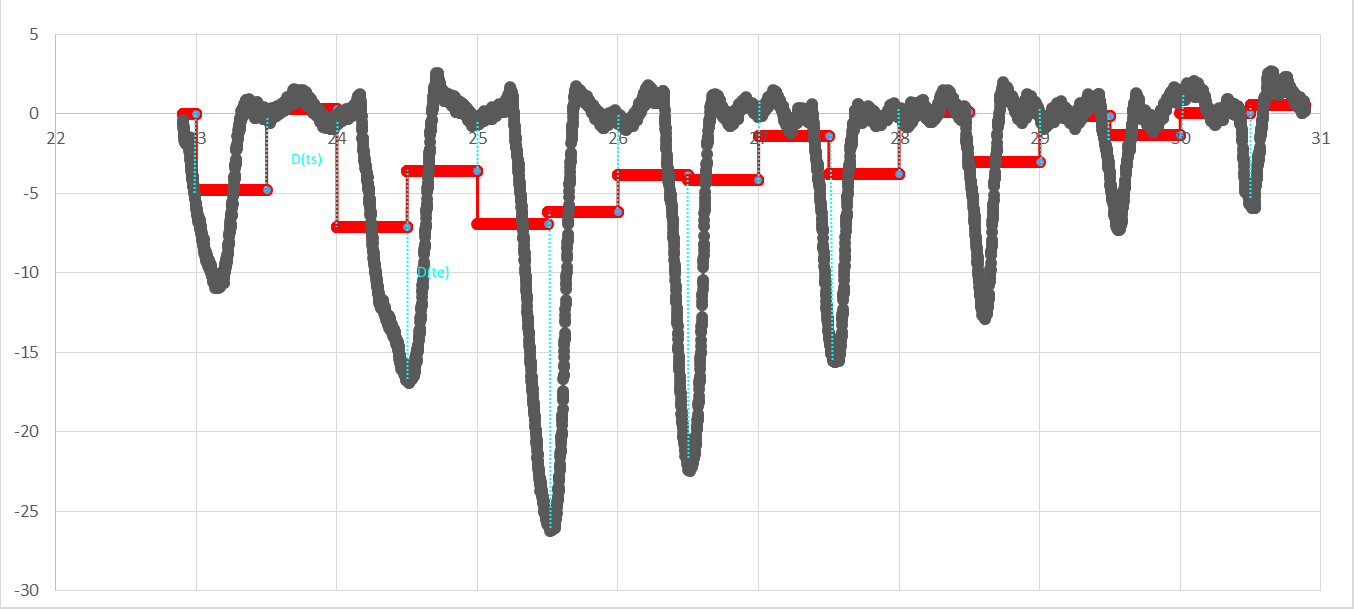
\includegraphics[scale=0.4]{images/sax-p/Sax-td}
    \caption{Trend Symbolic Aggregate approXimation of a cyclic time series}
  \label{fig:saxtd}
  \end{figure}
	
	 \begin{figure}[h]
  \centering
   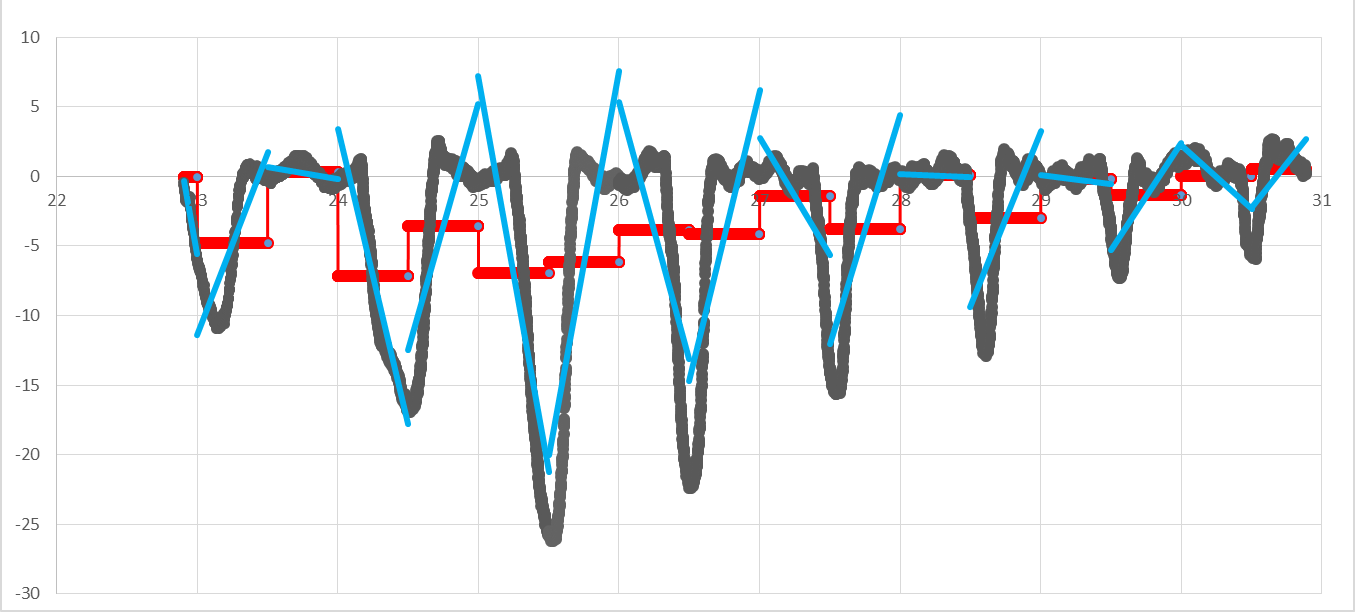
\includegraphics[scale=0.4]{images/sax-p/unD_sax}
    \caption{Properties of a cycle}
  \label{fig:1dsax}
  \end{figure}

Both methods provide better results than the SAX method \cite{sun2014improvement}. However, they have the
disadvantage of increasing the number of symbols required to represent the time series. Indeed, 
the method ESAX triple the size of the representation of a time series provided by the SAX method, 
while the SAX-TD method the double. In addition,  the previous four methods have two major drawbacks: 
they consider fixed-size segments, while the cycles are variable-sized segments, and they do not take into account the characteristic properties of cycles such as 
the duration and the surface under a cycle. Our goal is to provide a symbolic representation that 
takes into account several properties for each cycle, but without increasing the number of symbols 
used for the representation.


 The symbolic representations obtained have another advantage;
they allow to use a large number algorithms available
for sequence analysis like novelty detection (finding
unusual shapes or sub-sequences), motif discovery (finding
repeated shapes or sub-sequences) \cite{Begum2014}, clustering, classification,
indexing and also some interesting algorithms for
text processing or the bio-informatics community \cite{Aach2001, Papapetrou2011, Dietterich2002}. 

\section{SAX-P}

A prerequisite to be able to build a symbolic representation based on the cycles of the cyclic time series is to be able to segment the cyclic time series into consecutive cycles.

\subsection{Segmentation of cyclic time series}
The principle used to segment cyclic time series is as follows: A cycle contains all the data points between the beginning of two consecutive peaks. To locate the peaks, we set a threshold (Fig. \ref{fig:seuil}). The threshold considered can be the first or the second quartile of the time series data point.

	 \begin{figure}[h]
  \centering
   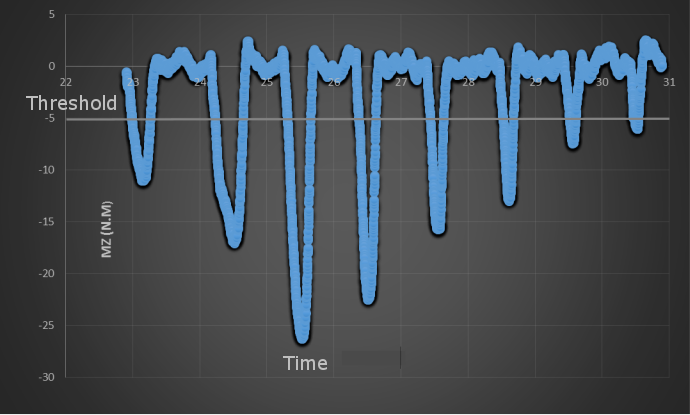
\includegraphics[scale=0.4]{images/sax-p/sax-p_deplacement_seuil}
    \caption{Threshold for the segmentation of cyclic time series}
  \label{fig:seuil}
  \end{figure}

If the current value of the time series is below this threshold, then it is a peak. It is then necessary to turn back to find the moment of the beginning of the peak. The figure (Fig. \ref{fig:segmentation}) presents the results obtained after segmentation of a cyclic time series.

	 \begin{figure}[h]
  \centering
   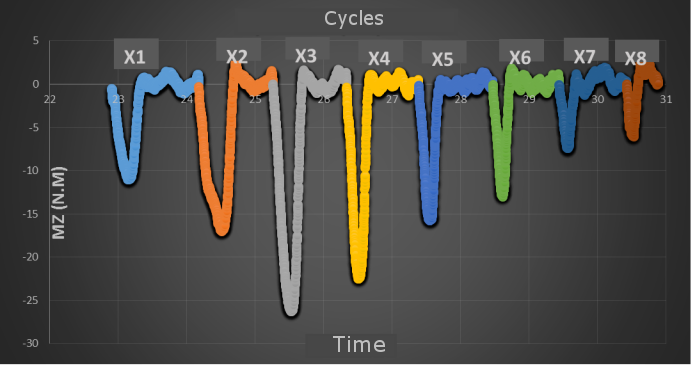
\includegraphics[scale=0.4]{images/sax-p/sax-p_deplacement32_thesee}
    \caption{Segmentation}
  \label{fig:segmentation}
  \end{figure}
	
\subsection{From cycles to letters}
The method SAX-P is based on SAX and works as follows:  
\begin{enumerate}
\item A cyclic time series is split in successive segments using a threshold
for identifying the beginning and the end of cycles, which have variable
durations;	
\item Several parameters (properties) are computed on each segment: cycle
time, push time, mean, median, standard deviation, minimum and maximum
values, and the area under the time series curve. As all these parameters
have different units, they must be normalized (i.e. centered and reduced) (Fig. \ref{fig:property} );

	 \begin{figure}[h]
  \centering
   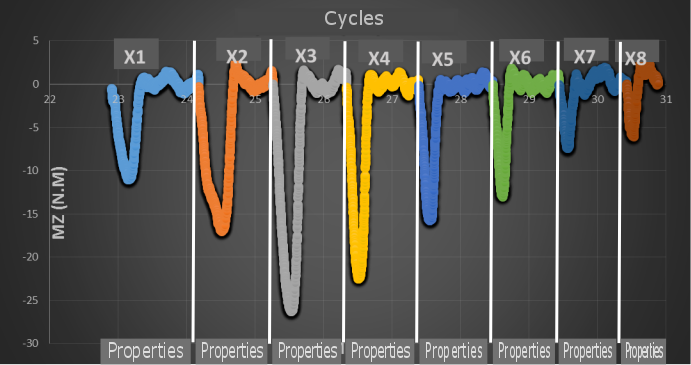
\includegraphics[scale=0.4]{images/sax-p/sax-p_deplacement_property}
    \caption{Some properties are computed on each cycle}
  \label{fig:property}
  \end{figure}
	
 
\item Segments are then gathered in clusters using a classification algorithm \\
\cite{Esling2012} and each cluster is named by a capital letter (Fig. \ref{fig:classification}); 

	 \begin{figure}[h]
  \centering
   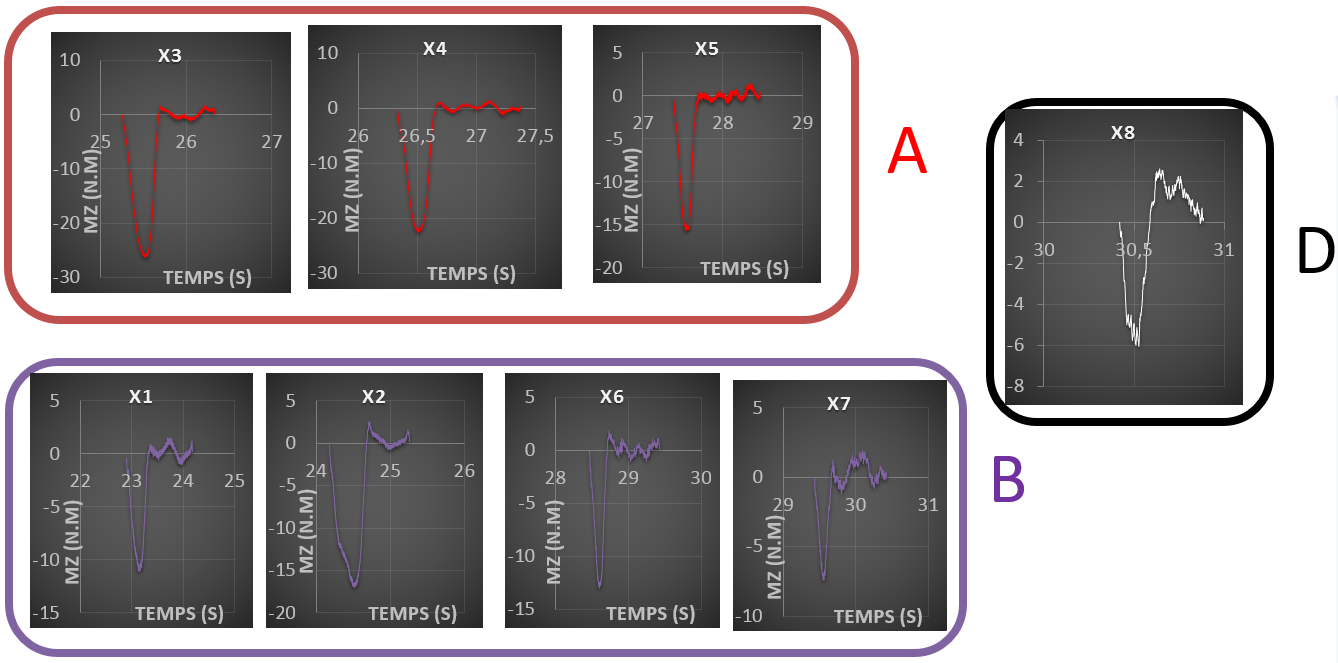
\includegraphics[scale=0.4]{images/sax-p/regroupement}
    \caption{Classification of cycles based on properties}
  \label{fig:classification}
  \end{figure}
	
	
\item Each segment is replaced by the letter of the cluster to which it
belongs, so that the initial cyclic time series is then represented
by a string of characters (Fig. \ref{fig:symbolic}); 

	 \begin{figure}[h]
  \centering
   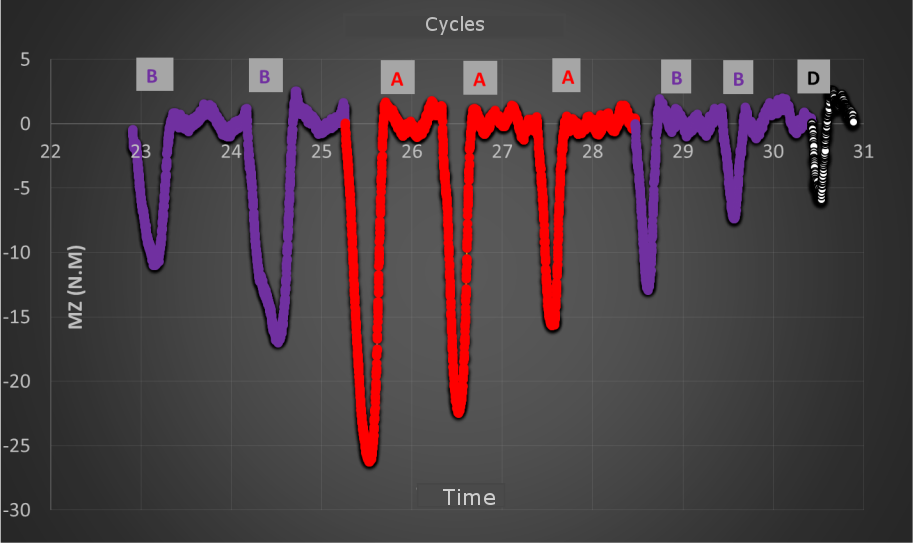
\includegraphics[scale=0.4]{images/sax-p/representionSymbolique2_t}
    \caption{Symbolic representation of cyclic time series}
  \label{fig:symbolic}
  \end{figure}
	
 \end{enumerate}

The distance between two strings, which may have different numbers
of characters, is computed using Dynamic Time Warping \cite{Petitjean2014} which is known as the
best distance measure for several domains \cite{Ding2008}. The distance between two characters is
the euclidean distance between the centers of the classes represented by those characters.

Unlike SAX, ESAX and SAX-TD methods that require  to fix the length of segments to consider when 
building the symbolic representation of a time series, SAX-P considers the cycles which
constitute basic unit of analysis of time series recorded during cyclic movements and also 
allows taking into account several characteristic features for each cycle. Figure \ref{fig:symbolic}
presents the symbolic representations obtained with the SAX method (in small letters) and SAX-P (in
capital letters). It illustrates that SAX-P unlike SAX considers cycles of the time series during
the construction of the symbolic representation.

%\begin{figure}[ht]
%\vskip 0.2in
%\begin{center}
%\centerline{\includegraphics[width=\columnwidth]{methode.png}}
%\caption{A cyclic time series is segmented in 5 propulsion cycles  
%(X1, X2, X3, X4, X5). For each cycle, a set of properties was 
%calculated and cycles with similar properties are gathered in 
%the same class (A or B). The original time series is thus transformed 
%into a string (here: AAABB).}
%\label{fig:methode}
%\end{center}
%\vskip -0.2in
%\end{figure} 

%\begin{figure}[ht]
%\vskip 0.2in
%\begin{center}
%\centerline{\includegraphics[width=\columnwidth]{representationS2.png}}
%\caption{Example of cyclic time series: propulsive moment applied by
% the subject S1  to the rear wheel of a Manual Wheelchair for a rectilinear
%  movement. Vertical bars delimit the propulsion cycles (segments) 
%  identified during this run, and the capital letter above each 
%  cycle indicates the cluster to which it belongs. Applying SAX to the propulsive moment divide
%  the time series into 10 segments of equal size (lowercase letter) regardless of propulsion cycles.
%  The area under the cycle, the cycle time and the pushed time are not taken into account by SAX.}
%\label{fig:moment}
%\end{center}
%\vskip -0.2in
%\end{figure} 

\section{Application to manual wheelchair locomotion}
This method has been applied to the axial moment (Mz) measured by both right and left rear wheels of
an instrumented Manual WheelChair (MWC) during five there and back 10-m linear displacements between
two cones performed by three handicapped subjects. We group propulsion cycles into 5 clusters  (Table
\ref{tab:centroide}) and we obtained a symbolic representation for Mz (Table
\ref{tab:symbole}).




\begin{table}
\center
\begin{tabular}{|c|c|c|c|c|c|}
\hline 
Cluster & A & B & C & D & E\tabularnewline
\hline 
\hline 
Nb of cycles & 18 & 36 & 59 & 18 & 104\tabularnewline
\hline 
\textbf{Cycle time (s)} & 1.2 & 1.0 & 1.0 & 1.7 & 0.8\tabularnewline
\hline 
\textbf{Push time (s)} & 0.6 & 0.3 & 0.4 & 1.0 & 0.3\tabularnewline
\hline 
Mz Min (Nm) & -22.3 & -17.4 & -11.4 & -8.7 & -6.4\tabularnewline
\hline 
Mz Max (Nm) & 0.1 & 0.1 & 0.1 & 0.7 & 0.1\tabularnewline
\hline 
Mean (Nm) & 13.6 & -8.1 & -6.2 & -3.0 & -3.3\tabularnewline
\hline 
Median (Nm) & -16.1 & -10.8 & -7.4 & -4.2 & -3.9\tabularnewline
\hline 
IRQ (Nm) & 12.4 & 10.7 & 6.0 & 4.3 & 3.1\tabularnewline
\hline 
SD (Nm) & 7.1 & 5.6 & 3.4 & 2.6 & 1.8\tabularnewline
\hline 
\textbf{Area (Nm.s)} & -7.1 & -2.3 & -2.2 & -1.8 & -1.0\tabularnewline
\hline 
\end{tabular}\protect\caption{Average vectors of the properties of classes (A, B, C, D, E) used
for the symbolic representation of the axial moment (Mz) SAX-P takes into account 
the surface under the push, the time-push and
the time-cycle.}
\label{tab:centroide}
\end{table}





\begin{center}

\begin{table}
\center
\begin{tabular}{|c|c|c|c|c|c|c|}
\hline 
Subject & \multicolumn{2}{c|}{S1} & \multicolumn{2}{c|}{S2} & \multicolumn{2}{c|}{S3}\tabularnewline
\hline 
\hline 
Push & Right & Left & Right & Left & Right & Left\tabularnewline
\hline 
1 & C & A & C & D & E & D\tabularnewline
\hline 
2 & B & B & E & E & D & E\tabularnewline
\hline 
3 & B & B & C & E & C & E\tabularnewline
\hline 
4 & B & B & C & E & E & E\tabularnewline
\hline 
5 & B & B & C & D & E & E\tabularnewline
\hline 
6 & C & B & E & C &  & D\tabularnewline
\hline 
7 & B & C & E & E &  & E\tabularnewline
\hline 
8 & E &  & E & E &  & \tabularnewline
\hline 
9 &  &  & C & C &  & \tabularnewline
\hline 
10 &  &  & E & E &  & \tabularnewline
\hline 
11 &  &  & C & E &  & \tabularnewline
\hline 
12 &  &  & C & E &  & \tabularnewline
\hline 
13 &  &  &  & E &  & \tabularnewline
\hline 
DTW & \multicolumn{2}{c|}{268} & \multicolumn{2}{c|}{354} & \multicolumn{2}{c|}{44}\tabularnewline
\hline 
\end{tabular}

\protect\caption{Strings of characters obtained with SAX-P method on times series of
axial moments applied by the three subjects on right and left rear
wheels of an instrumented MWC during their second 10-m run.}
\label{tab:symbole}

\end{table}

\end{center}





An important task of analyzing manual wheelchair locomotion 
 is the comparison of its rolling movement. Experts from the fields seek to 
 compare two movements simultaneously taking into account 
 several criteria or properties. Applying SAX-P method to the time series 
 of axial moments exerted
by a wheelchair user on the right and left wheels greatly
facilitates the comparison, the analysis and the interpretation of these time series: 
\begin{itemize}
\item At first sight (Table 2), it immediately appears that during their
second 10-m run the three subjects analyzed here did not exert the
same number of pushes for moving a MWC on the same distance (S1:
7-8; S2: 12-13; S3: 5-7); 
\item It is also obvious that each subject did not exert the same number
of pushes on both rear wheels. Moreover, although right and left pushes
exerted by one subject globally belong to the same clusters, the total
distance between all these pushes can be more (S2: 354) or less (S3:
44) high. Both these observations clearly demonstrate that the three
subjects did not propel their MWC symmetrically during this particular
exercise. The first results of the evaluation of SAX-P on a classification task are presented on
the web page \cite{Validation}
\end{itemize}


\section{Conclusion}
In this ongoing work, we proposed a method of symbolic representation of cyclic time series called SAX-P.
This method is used to represent a cyclic time series as a string, each character representing a
class of the cycles of the considered time series. The character strings
obtained were then compared using the Dynamic Time Warping distance.
 The SAX-P model has been applied to propulsive moments measured during the movements in a straight
 line by three subjects in MWC. The preliminary results obtained have particularly showed that these
 subjects had different modes of propulsion and propulsion cycles of the same subject were not 
 symmetrical. Ongoing research is devoted on applying this new symbolic representation to a 
 supervised classification of cyclic time-series in bio-mechanics.
 
 
 \begin{table}[ht]
\centering
\begin{tabular}{|l|}

\hline
\rowcolor{LavenderBlush}
Key points\\
$\bullet$ We propose a symbolic representation of cyclic time series based \\ on the properties of the cycles. \\
\\
$\bullet$ We show that this symbolic representation improves the \\ visualization and processing of cyclic time series from manual wheelchair locomotion.\\ 
\\
Communications :\\
$-$ Siyou Fotso VS, Mephu-Nguifo E, Vaslin Ph. Symbolic representation of cyclic\\ time series: application to biomechanics. Constructive Machine Learning \\workshop at International Conference on Machine Learning , France, July 2015\\

$-$ Siyou Fotso VS, Mephu-Nguifo E, Vaslin Ph. Représentation symbolique de \\ séries temporelles cycliques basée sur les propriétés des cycles : application \\ à la biomécanique . Treizièmes Rencontres des Jeunes Chercheurs en Intelligence \\ Artificielle (RJCIA 2015), Rennes, France, Jun 2015\\

$-$ Siyou Fotso VS, E. M. Nguifo, and P. Vaslin, “Symbolic representation of \\propulsion cycles in manual wheelchair locomotion,” Comput. Methods \\ Biomech. Biomed. Engin., vol. 18, no. sup1, pp. 2060–2061, 2015.\\

$-$ C. Sauret, Siyou Fotso VS, J. Bascou, H. Pillet, E. Mephu-Nguifo, P. Fodé, \\and P. Vaslin, “Cluster analysis to investigate biomechanical changes during learning \\ of manual wheelchair locomotion: a preliminary study,” Comput. Methods Biomech.\\ Biomed. Engin., vol. 18, no. sup1, pp. 2058–2059, 2015.\\

 
\hline
\end{tabular}
\end{table}
\chapter[Application]{Application to manual wheelchair locomotion}
\label{application}
\section{Introduction}
The moment of a force around an axis is a physical vector quantity, which measures the ability of the force to rotate a solid around an axis. In the case of wheelchair locomotion, the moment measures a subject's ability to turn the wheels of his Wheelchair, that is, to move with his Wheelchair. It is, therefore, a quantity whose measurement is essential for the analysis of locomotion in a Manual Wheelchair. With this in mind, a sensor capable of measuring wheel moment was installed on the field-ergometer manual wheelchair.  In this chapter, we will analyse the measurements made by this sensor to understand manual wheelchair locomotion better. To do this, we will first present the moment-sensor, then the data sets that are the subject of our analyses. We will then revisit the classic questions of manual wheelchair locomotion: the symmetry of manual wheelchair locomotion, the evaluation of the propulsion capacities of subjects in manual wheelchairs.

\section{The torsor sensor}

A torsor is a mathematical object used to characterize the movements of a solid. It measures both the forces and moments applied to this object along three axes. A torsor sensor was designed, built and installed on the wheels of the field-ergometer manual wheelchair (Fig. \ref{capteur_tri_axe}), to measure the forces exerted by wheelchair users during their locomotion.

\begin{figure}[h]
\center
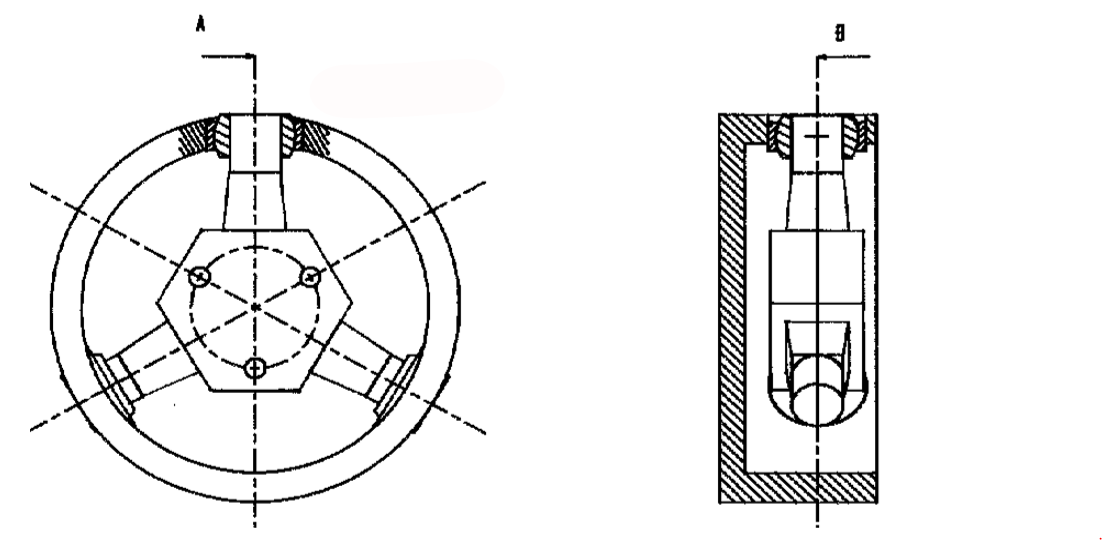
\includegraphics[scale = 0.4]{images/capteur_tri_axe}
\caption{Torsor sensor, brevet WO 1995001556 A1}
\label{capteur_tri_axe}
\end{figure}

It consists of three bidirectional sensors measuring the forces applied to the handrail.

\section{Description of  datasets}
The data sets we use throughout these tests are from experiments that were conducted with subjects with disabilities; here, the measurements were intended to understand manual wheelchair locomotion and also to evaluate the mechanical stresses it exerts on manual wheelchair users. In the other case, experiments were conducted with valid subjects. Here, the objective was to measure the impact of the experience on the propulsion technique used by the subjects. 


In both cases, the measurements made produce noisy, cyclic and uncertain time series (Fig. \ref{TWMWC}). All subsequent treatments are performed on the Z moment measured on the wheels of a manual wheelchair field ergometer.

\begin{figure}[h]
\center
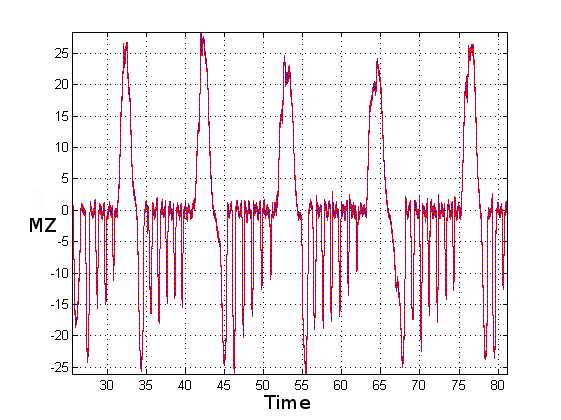
\includegraphics[scale = 0.5]{images/TSMWC}
\caption{Example of Z moment from a wheel of a  field-ergometer manual wheelchair}
\label{TWMWC}
\end{figure}


We want to return to the characteristic properties of the Z moments measured by the torsor sensor and explain why the recorded measurements are long, noisy, cyclic and uncertain.

\paragraph{Length of time series:} the length of the time series is due to the high acquisition frequency of the torsor sensor. The acquisition frequency is 100Hz in other words; the sensor makes 100 measurements per second. Thus, a 10-minute recording generates a time series of $100 \times 60 \times 10 = 60,000$ data points. As another example is the Z moment of the left wheel of subject S02 has $107 227$ data points (Fig. \ref{mz_left_wheel}). The length of time series is problematic because the processing time of time series is highly dependent on their length. As an illustration, the time complexity of comparing two time series using the DTW alignment algorithm is $O(n^2)$ where $n$ is the length of the time series.

\begin{figure}[h]
\center
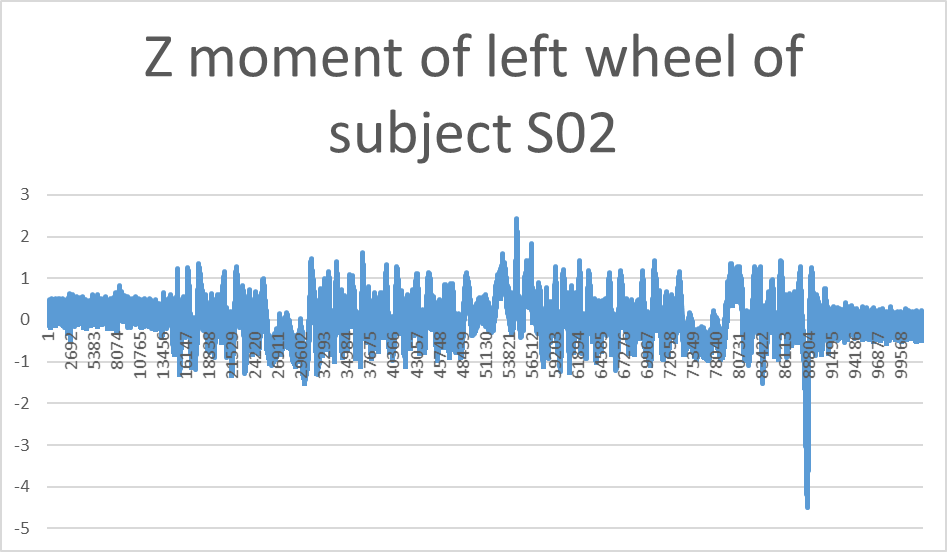
\includegraphics[scale = 0.6]{images/mz_left_wheel}
\caption{Z moment of the left wheel of manuel wheelchair recorded during the locomotion of subject S02}
\label{mz_left_wheel}
\end{figure}


\paragraph{Noise in time series:} The time series noise comes from the sensitivity of the torsor sensor which measures low-intensity forces applied to the handrail during manual wheelchair locomotion. These forces can come from the texture of the ground, the friction of the arm on the handrail during the movement or other. Noise in time series is problematic because it influences the calculation of the distance between two time-series, the division into cycles of a cyclic time series, or even the computation of properties that can characterize a time series.

\begin{figure}[h]
\center
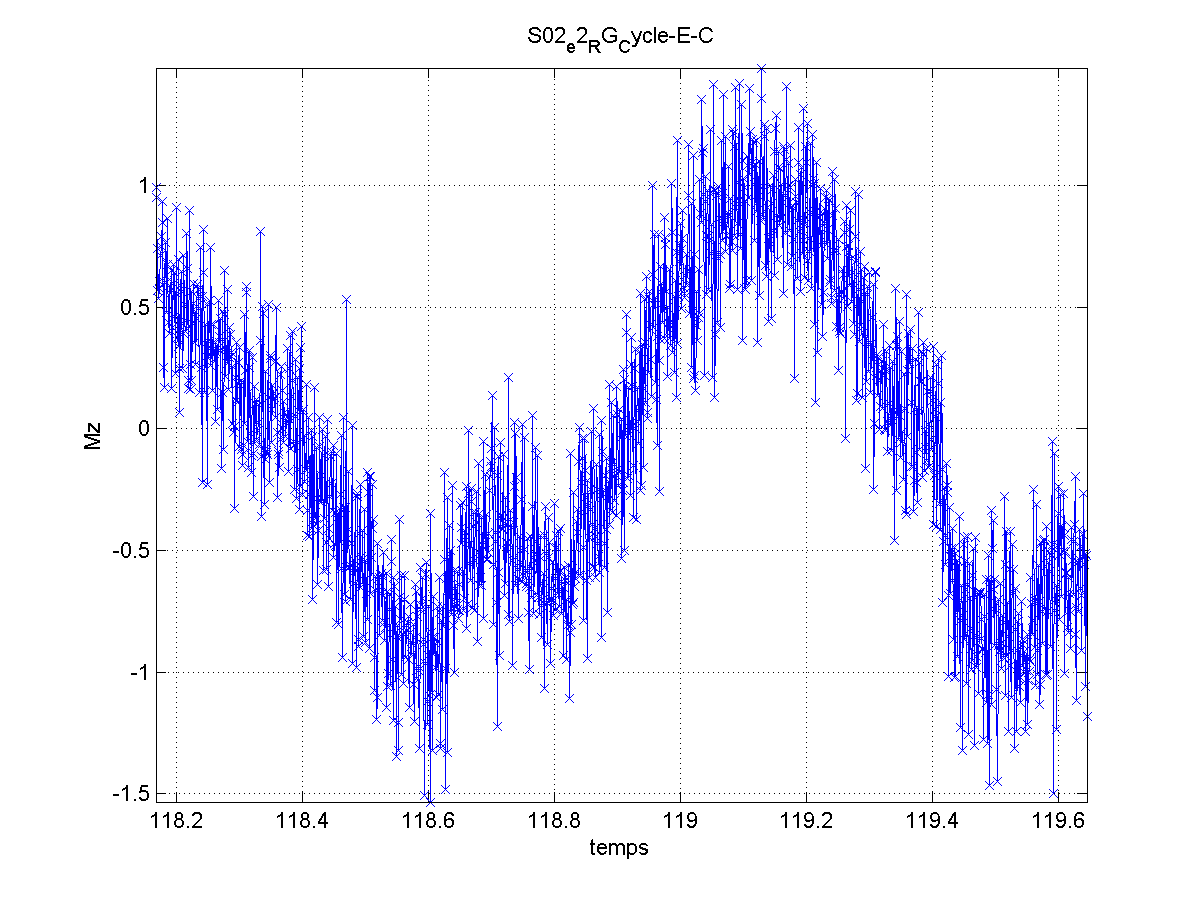
\includegraphics[scale = 0.5]{images/TSN}
\caption{Time series recorded by torsor sensor are noisy}
\label{TWMWC}
\end{figure}

\paragraph{Cycles in time series:} The cyclical aspect of the time series comes from the cyclical nature of the movement in the Manual Wheelchair. Indeed, manual wheelchair movement consists of a succession of push moments during which the user of the manual wheelchair applies a force on the handrail of the wheelchair to move it and freewheel moment, instant during which the user of the manual wheelchair rests and takes momentum for the next push. The push is recorded by the sensor and materialized by a peak in the measurements, the periods of freewheel correspond to the values close to zero(Fig. \ref{TWMWC}). 

\paragraph{Uncertainty in time series :} The presence of uncertainty in sensor measurements is not a myth; it is a reality. To realize it, it is necessary to first understand the calibration process of the sensors in general, and of the torsor sensor in the case of this work. 
There are two leading families of sensors: piezo-resistive and piezo-electric, that have a similar operating principle. When a force is applied to the sensor, it causes a deformation of the sensor which induces a change in its resistance in the case of the piezo-resistive sensor or a change in the electrical voltage at its terminals, as is the case with piezoelectric sensors. The functioning of the sensor is based on the assumption that the change in resistance or electrical voltage induced by the force is proportional to the intensity of the force. Thus, the  sensor measures variation in resistance or electrical voltage and uses the proportionality relationship to infer the intensity of the force that has been applied. Calibrating a sensor consists in constructing this proportionality relation by applying greater and greater or smaller and smaller forces on the sensor. Doing so, we record a sequence of couples of force intensity, electrical voltage (or resistance) which is used to plot a regression line which will then be used to deduct the applied force knowing the voltage intensity  variation. However, the regression line does not define a perfect proportionality relationship. In fact, it minimizes the error made but does not cancel it. This error (Fig. \ref{residus}) introduces uncertainty into the estimation of the applied force intensity. It is essential to take this error into account when processing time series to extract relevant information from them.
Characterization of uncertainty is a time-consuming task (Appendix .\ref{pdf_uncertainty}) and is not always possible because sensor calibration data are generally not available. We, therefore, chose during these experiments to consider strategies that did not require knowledge of the probability distribution of uncertainty.

\begin{figure}[h]
\center
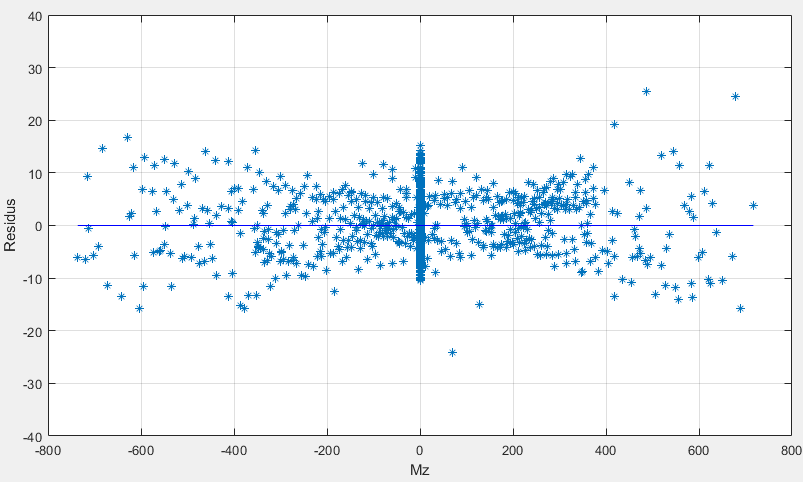
\includegraphics[scale = 0.5]{images/residus}
\caption{Residus of Mz; they represents difference between the real value and the value measured by the sensor.}
\label{residus}
\end{figure}

We will then explain how we use this data for the analysis of Manual Wheelchair locomotion. We remove noise on time series using a moving average filter. However, we don’t compress the time series using FDTW because we don’t have classes labels. 

\section{Manual Wheelchair locomotion analysis}

\subsection{Preprocessing}
Removing the noise contained in the time series and reducing their length are prerequisites to its operation for the analysis of manual wheelchair locomotion.

\subsection{Exploitation of time series of rolling chair locomotion}

\subsubsection{The symmetry of Manual Wheelchair Locomotion}
For a long time, experts assumed that the Manual Wheelchair locomotion was symmetrical, which made it possible to construct measuring instruments consisting of a single wheel \cite{brouha1967continuous}. Subsequently, the conclusions that were drawn from the measurements made with one wheel were generalized to both upper limbs of the subject. Then \cite{langbein1993research} built a roller ergometer capable of separately measuring the speed and resistance of the left and right wheels of the Manual Wheelchair during its use. The measurements taken from this roller ergometer revealed a difference between the properties measured by the left and right wheels and allowed the asymmetric character of the Manual Wheelchair locomotion to be deduced. In this paragraph, we use the SAX-P symbolic representation and the additional information we have on the subjects to carry out a new analysis of the symmetry of manual wheelchair locomotion.


As we have already demonstrated in chapter \ref{chapter_saxp}, even if a user of a Manual Wheelchair makes the same number of pushes with the right and left wheels during a straight line movement, these cycles may have different properties, which in our case takes the form of different letters in the character strings corresponding to the right and left wheels. This asymmetry of the locomotion in the Manual Wheelchair can be evaluated by calculating a relative Edit distance between the characters strings that correspond to the straight line displacements of the of the right and left wheels. The relative Edit distance counts the number of different letters between two characters strings.

\[
D(X,Y)=\frac{1}{n}\stackrel[i=1]{n}{\sum}[X_{i}\neq Y_{i}]
\]









\begin{longtable}
   {|p{0.35\linewidth}|p{0.2\linewidth}|p{0.1\linewidth}|}
   
   \hline
\multicolumn{1}{|l|}{\textbf{Subject}} & \multicolumn{1}{|l|}{\textbf{Straight displacement}} & \multicolumn{1}{|l|}{\textbf{Relative Edit Distance}}\endfirsthead 
 \hline

\multicolumn{1}{|l|}{\textbf{Subject}} & \multicolumn{1}{|l|}{\textbf{Straight displacement}} & \multicolumn{1}{|l|}{\textbf{Relative Edit Distance}}  \\

	 \hline
   \multicolumn{3}{|p{0.65\linewidth}|}{Following ... } \\

   \hline
	 \endhead

   \hline
   \multicolumn{3}{|p{0.65\linewidth}|}{Continue to the next page}\\ 

	 \hline 
	 \endfoot 

	 \hline
   \multicolumn{3}{|p{0.65\linewidth}|}{End} \\

   \hline
   \endlastfoot 
	\hline
S02\_e1\_RD\_H4-Cycle-A                & AAAAAA                                              & 0,17\\
S02\_e1\_RG\_H4-Cycle-A                & AAAAA                                               &\\
S02\_e1\_RD\_H4-Cycle-B                & AAAAAAAAAAAAA                                       &0,06\\
S02\_e1\_RG\_H4-Cycle-B                & AAAAAAAAAAAA                                        &\\
S02\_e1\_RD\_H4-Cycle-C                & AAAAAAAAAAA                                         &0\\
S02\_e1\_RG\_H4-Cycle-C                & AAAAAAAAAAA                                         &\\
S02\_e1\_RD\_H4-Cycle-D                & AAAAAAA                                             &0\\
S02\_e1\_RG\_H4-Cycle-D                & AAAAAAA                                             &\\
Moyenne                                &                                                     & 0,05\\
&&\\
S03\_E3\_T\_RD-Cycle-A                 & EEBCB                                               & 0,40                                                  \\
S03\_E3\_T\_RG-Cycle-A                 & EEECC                                               &                                                       \\
S03\_E3\_T\_RD-Cycle-B                 & BBBBCB                                              & 0,33                                                  \\
S03\_E3\_T\_RG-Cycle-B                 & EBBBCC                                              &                                                       \\
S03\_E3\_T\_RD-Cycle-C                 & EBBBBBC                                             & 0,17                                                  \\
S03\_E3\_T\_RG-Cycle-C                 & EBBBBCC                                             &                                                       \\
S03\_E3\_T\_RD-Cycle-D                 & EBCBC                                               & 0,86                                                  \\
S03\_E3\_T\_RG-Cycle-D                 & EEECBCC                                             &                                                       \\
S03\_E3\_T\_RG-Cycle-E                 & EBBBBBC                                             & 0,29                                                  \\
S03\_E3\_T\_RD-Cycle-E                 & EBEBBCC                                             &                                                       \\
S03\_E3\_T\_RD-Cycle-F                 & EEEBBCC                                             & 0,43                                                  \\
S03\_E3\_T\_RG-Cycle-F                 & EEECCCD                                             &                                                       \\
S03\_E3\_T\_RG-Cycle-G                 & EEBCCC                                              & 0,57                                                  \\
S03\_E3\_T\_RD-Cycle-G                 & BEECBCC                                             &                                                       \\
S03\_E3\_T\_RD-Cycle-H                 & EEBCBCC                                             & 0,29                                                  \\
S03\_E3\_T\_RG-Cycle-H                 & EBBBBCC                                             &                                                       \\
S03\_E3\_T\_RG-Cycle-I                 & CC                                                  & 1,00                                                  \\
S03\_E3\_T\_RD-Cycle-I                 & BBD                                                 &                                                       \\
Moyenne                                &                                                     & 0.48                                                  \\
                                       &                                                     &                                                       \\
S04\_E1\_T\_RD-Cycle-A                 & EEDBBCCC                                            & 0,38                                                  \\
S04\_E1\_T\_RG-Cycle-A                 & DEEBBCCA                                            &                                                       \\
S04\_E1\_T\_RG-Cycle-B                 & EEBDACC                                             & 0,63                                                  \\
S04\_E1\_T\_RD-Cycle-B                 & BBBBCCCC                                            &                                                       \\
S04\_E1\_T\_RD-Cycle-C                 & ECBCCCC                                             & 0,57                                                  \\
S04\_E1\_T\_RG-Cycle-C                 & BBECCC                                              &                                                       \\
S04\_E1\_T\_RG-Cycle-D                 & EBBCC                                               & 0,57                                                  \\
S04\_E1\_T\_RD-Cycle-D                 & EBBBBBC                                             &                                                       \\
S04\_E1\_T\_RD-Cycle-E                 & EBBC                                                & 0,50                                                  \\
S04\_E1\_T\_RG-Cycle-E                 & EBC                                                 &                                                       \\
S04\_E1\_T\_RD-Cycle-F                 & EBC                                                 & 0,33                                                  \\
S04\_E1\_T\_RG-Cycle-F                 & BBC                                                 &                                                       \\
Moyenne                                &                                                     & 0.5                                                   \\
                                       &                                                     &                                                       \\
S05\_E3\_T\_RD-Cycle-A                 & BBBBCDD                                             & 0,86                                                  \\
S05\_E3\_T\_RG-Cycle-A                 & EEBDBCA                                             &                                                       \\
S05\_E3\_T\_RD-Cycle-B                 & BBCDCDBC                                            & 0,63                                                  \\
S05\_E3\_T\_RG-Cycle-B                 & BBBCCA                                              &                                                       \\
S05\_E3\_T\_RD-Cycle-C                 & EDDDDDCAD                                           & 0,78                                                  \\
S05\_E3\_T\_RG-Cycle-C                 & BBBCBCA                                             &                                                       \\
S05\_E3\_T\_RD-Cycle-D                 & BBCCDCA                                             & 0,29                                                  \\
S05\_E3\_T\_RG-Cycle-D                 & BBCBCCA                                             &                                                       \\
S05\_E3\_T\_RD-Cycle-E                 & BBBCDCCD                                            & 0,75                                                  \\
S05\_E3\_T\_RG-Cycle-E                 & BCDDCDA                                             &                                                       \\
S05\_E3\_T\_RD-Cycle-F                 & BCBDCDCD                                            & 0,63                                                  \\
S05\_E3\_T\_RG-Cycle-F                 & DBBCDDAD                                            &                                                       \\
S05\_E3\_T\_RD-Cycle-G                 & BC                                                  & 1,00                                                  \\
S05\_E3\_T\_RG-Cycle-G                 & DA                                                  &                                                       \\
Moyenne                                &                                                     & 0.70                                                  \\
                                       &                                                     &                                                       \\
S07\_e1\_T\_RD-Cycle-A                 & AEDBDA                                              & 0,33                                                  \\
S07\_e1\_T\_RG-Cycle-A                 & EEBBD                                               &                                                       \\
S07\_e1\_T\_RG-Cycle-B                 & BBCCC                                               & 0,00                                                  \\
S07\_e1\_T\_RD-Cycle-B                 & BBCCC                                               &                                                       \\
S07\_e1\_T\_RD-Cycle-C                 & ECDADAA                                             & 0,71                                                  \\
S07\_e1\_T\_RG-Cycle-C                 & EBCCD                                               &                                                       \\
S07\_e1\_T\_RG-Cycle-D                 & BBBCCD                                              & 0,57                                                  \\
S07\_e1\_T\_RD-Cycle-D                 & EBCCADA                                             &                                                       \\
S07\_e1\_T\_RD-Cycle-E                 & EBCCCAD                                             & 0,57                                                  \\
S07\_e1\_T\_RG-Cycle-E                 & BBBCCC                                              &                                                       \\
S07\_e1\_T\_RD-Cycle-F                 & BC                                                  & 1,00                                                  \\
S07\_e1\_T\_RG-Cycle-F                 & EC                                                  &                                                       \\
Moyenne                                &                                                     & 0.53                                                  \\
                                       &                                                     &                                                       \\
S08\_e3\_T\_RD-Cycle-A                 & DDDDDAD                                             & 0,29                                                  \\
S08\_e3\_T\_RG-Cycle-A                 & DDDDDDA                                             &                                                       \\
S08\_e3\_T\_RD-Cycle-B                 & DDDADDDDAA                                          & 0,40                                                  \\
S08\_e3\_T\_RG-Cycle-B                 & BDDDDAADAA                                          &                                                       \\
S08\_e3\_T\_RD-Cycle-C                 & DDDDDDDDA                                           & 0,67                                                  \\
S08\_e3\_T\_RG-Cycle-C                 & AAADAADAA                                           &                                                       \\
S08\_e3\_T\_RD-Cycle-D                 & DDDDDDDDC                                           & 0,89                                                  \\
S08\_e3\_T\_RG-Cycle-D                 & AAADAAAAA                                           &                                                       \\
S08\_e3\_T\_RD-Cycle-E                 & BDDD                                                & 0,50                                                  \\
S08\_e3\_T\_RG-Cycle-E                 & DDDA                                                &                                                       \\
Moyenne                                &                                                     & 0.55                                                  \\
                                       &                                                     &                                                       \\
S09\_e1\_T\_RD-Cycle-A                 & DADDDA                                              & 0,33                                                  \\
S09\_e1\_T\_RG-Cycle-A                 & DDDADA                                              &                                                       \\
S09\_e1\_T\_RD-Cycle-B                 & DDAADAAAAA                                          & 0,92                                                  \\
S09\_e1\_T\_RG-Cycle-B                 & AADDDDDDDDAA                                        &                                                       \\
S09\_e1\_T\_RD-Cycle-C                 & DDAAADADD                                           & 0,40                                                  \\
S09\_e1\_T\_RG-Cycle-C                 & DDADDDCDDA                                          &                                                       \\
S09\_e1\_T\_RD-Cycle-D                 & DDDDAAA                                             & 0,70                                                  \\
S09\_e1\_T\_RG-Cycle-D                 & AADDDDADAA                                          &                                                       \\
Moyenne                                &                                                     & 0.59                                                  \\
                                       &                                                     &                                                       \\
S10\_e3\_RD\_H-4-Cycle-A               & EEBC                                                & 0,20                                                  \\
S10\_e3\_RG\_H-4-Cycle-A               & EEBCD                                               &                                                       \\
S10\_e3\_RD\_H-4-Cycle-B               & EBDCCA                                              & 0,83                                                  \\
S10\_e3\_RG\_H-4-Cycle-B               & BBBBCC                                              &                                                       \\
S10\_e3\_RD\_H-4-Cycle-C               & EBBCCCD                                             & 0,29                                                  \\
S10\_e3\_RG\_H-4-Cycle-C               & BBBCCCC                                             &                                                       \\
S10\_e3\_RD\_H-4-Cycle-D               & EECCCA                                              & 0,67                                                  \\
S10\_e3\_RG\_H-4-Cycle-D               & BBBCCC                                              &                                                       \\
S10\_e3\_RD\_H-4-Cycle-E               & EBCCDC                                              & 0,50                                                  \\
S10\_e3\_RG\_H-4-Cycle-E               & BBBCCC                                              &                                                       \\
S10\_e3\_RD\_H-4-Cycle-F               & CAAAEB                                              & 0,86                                                  \\
S10\_e3\_RG\_H-4-Cycle-F               & BCDCABC                                             &                                                       \\
S10\_e3\_RD\_H-4-Cycle-G               & C                                                   & 0,50                                                  \\
S10\_e3\_RG\_H-4-Cycle-G               & CE                                                  &                                                       \\
Moyenne                                &                                                     & 0.55                                                  \\
                                       &                                                     &                                                       \\
S11\_e1\_T\_RD-Cycle-A                 & BDDA                                                & 0,50                                                  \\
S11\_e1\_T\_RG-Cycle-A                 & BBD                                                 &                                                       \\
S11\_e1\_T\_RD-Cycle-B                 & DDDDADDA                                            & 0,38                                                  \\
S11\_e1\_T\_RG-Cycle-B                 & BBDBADDA                                            &                                                       \\
S11\_e1\_T\_RD-Cycle-C                 & DDDADADA                                            & 0,50                                                  \\
S11\_e1\_T\_RG-Cycle-C                 & BDDDDDDD                                            &                                                       \\
S11\_e1\_T\_RD-Cycle-D                 & BDDDAAAA                                            & 0,50                                                  \\
S11\_e1\_T\_RG-Cycle-D                 & BDDDDDDD                                            &                                                       \\
S11\_e1\_T\_RD-Cycle-E                 & DA                                                  & 0,67                                                  \\
S11\_e1\_T\_RG-Cycle-E                 & DDD                                                 &                                                       \\
Moyenne                                &                                                     & 0.51                                                  \\
                                       &                                                     &                                                       \\
S12\_e2\_RD\_H4-Cycle-A                & DDDAAAA                                             & 0,71                                                  \\
S12\_e2\_RG\_H4-Cycle-A                & BDDDDD                                              &                                                       \\
S12\_e2\_RD\_H4-Cycle-B                & DADDDAAAA                                           & 0,44                                                  \\
S12\_e2\_RG\_H4-Cycle-B                & AADDDDADD                                           &                                                       \\
S12\_e2\_RD\_H4-Cycle-C                & DDAADADDAAAA                                        & 0,67                                                  \\
S12\_e2\_RG\_H4-Cycle-C                & DBDDDDDDDDDD                                        &                                                       \\
S12\_e2\_RD\_H4-Cycle-D                & DDAADD                                              & 0,50                                                  \\
S12\_e2\_RG\_H4-Cycle-D                & DDADD                                               &                                                       \\
Moyenne                                &                                                     & 0.58 \\ \hline  
\caption{Straight displacement in manual wheelchair}
\label{dw}                                              
\end{longtable}



We observe that the asymmetry of Manual Wheelchair locomotion is not the same for all subjects. Indeed, it is zero for subject S02 who has only carried out type A pushes throughout his movements, but it is very important (0.7) for subject S05. We then want to know what factors might influence asymmetry of locomotion. We then cross-referenced the previous results with the number of years of Manuals wheelchair locomotion practice of the subjects who participated in the experiment (Tab. \ref{dissymmetry}).

\begin{table}[h]
\centering
\begin{tabular}{|l|l|l|}
\hline
\multicolumn{1}{|l|}{\textbf{Subject}} & \multicolumn{1}{l|}{\textbf{Edit distance}} & \multicolumn{1}{l|}{\textbf{Duration of practice}} \\ \hline
S02 & 0.05 & 33 years         \\
S03 & 0.43 & 7 years          \\
S04 & 0.5  & 6 months         \\
S11 & 0.51 & 12 years         \\
S07 & 0.53 & 7 months 6 days  \\
S08 & 0.55 & 3 years 6 months \\
S10 & 0.55 & 2 years          \\
S12 & 0.58 & 11 months        \\
S09 & 0.59 & 9 months         \\
S05 & 0.7  & 2 months         \\
\hline                                             
\end{tabular}
\caption{Dissymmetry and number of years of practice}
\label{dissymmetry}
\end{table}




We observe that the subject S05 who has the least experience in the use of the Manual Wheelchair (2 months) has very asymmetric propulsion (0.7) whereas the subject S02 who has a vast experience in the use of the wheelchair (33 years) has an almost symmetrical propulsion (0.05). We calculated the correlation of Pearson between the dissymmetry and the number of years of use of the Manual Wheelchair. We obtain a correlation coefficient c = -0.928. 



These results suggest that the more experience subjects have in using the Manual Wheelchair, the more symmetrical its propulsion will be when moving in a straight line. 


\subsubsection{Group Manual Wheelchair users according to their motor skills}

It is essential to be able to group wheelchair users according to their motor abilities. In the context of the Paralympic Games, this classification makes it possible to form teams based on functional and not physiological criteria and thus to guarantee that competition is fairer. The assessment of motor skills can, however, be subjective, as it is sometimes based on observation of matches, or on a test set offered to the subject in a Manual Wheelchair. In both cases, it is an expert who appreciates the mobility of the subjects by scoring it on a scale. In this section, we present a different, more objective approach for comparing Manual Wheelchair users based on measurements made during their use of the chair. We want that the method used for the evaluation of motor abilities remains understandable by experts in the field. The experiments presented in this section were performed on measurements from manual wheelchair locomotion of 11 subjects with different physiological characteristics: sex, weight, height, age, level of spinal injury. Table \ref{physio} details the physiological characteristics of the patients. 

\begin{landscape}

\begin{table}[h]
\centering
\begin{tabular}{|c|c|c|c|c|c|c|c|c|c|c|c|}
\hline
\multicolumn{1}{|c|}{ \textbf{\begin{tabular}[c]{@{}c@{}}\end{tabular}}      } & \multicolumn{1}{c|}{\textbf{F/M}} & \multicolumn{1}{c|}{\textbf{Age}} & \multicolumn{1}{c|}{  \textbf{\begin{tabular}[c]{@{}c@{}}H.\\  (cm)\end{tabular}}} & \multicolumn{1}{c|}{  \textbf{\begin{tabular}[c]{@{}c@{}}W.\\  (kg)\end{tabular}}} & \multicolumn{1}{c|}{\textbf{\begin{tabular}[c]{@{}c@{}}Dominant\\  Membre\end{tabular}}} & \multicolumn{1}{c|}{\textbf{\begin{tabular}[c]{@{}c@{}} injury\end{tabular}}} & \multicolumn{1}{c|}{\textbf{\begin{tabular}[c]{@{}c@{}}Affected\\ Vertebrae\end{tabular}}} & \multicolumn{1}{c|}{\textbf{\begin{tabular}[c]{@{}c@{}}Severity \end{tabular}}} & \multicolumn{1}{c|}{\textbf{\begin{tabular}[c]{@{}c@{}}Experience\\ (years)\end{tabular}}} & \multicolumn{1}{c|}{\textbf{\begin{tabular}[c]{@{}c@{}}hours /\\   day\end{tabular}}} & \multicolumn{1}{c|}{\textbf{\begin{tabular}[c]{@{}c@{}}days /\\   week\end{tabular}}} \\ \hline
S2                                                     & F                                   & 33                                & 162                                       & 50                                        & Right                                                                                    & Cervical                                                                                 & C5-C6                                                                                      & Complet                                                                                     & 33                                                                                              &                                                                                            & 1                                                                                          \\ \hline
S3                                                     & M                                   & 34                                & 178                                       & 78                                        & Right                                                                                    & Thoracic                                                                                 & D4-D5                                                                                      & Complet                                                                                     & 7                                                                                               & 14                                                                                         & 6                                                                                          \\ \hline
S4                                                     & M                                   & 47                                & 180                                       & 80                                        & Right                                                                                    & Thoracic                                                                                 & D8                                                                                         & Complet                                                                                     & 0,5                                                                                             & 5                                                                                          & 7                                                                                          \\ \hline
S5                                                     & M                                   & 48                                & 170                                       & 66                                        & Left                                                                                     & Thoracic                                                                                 & D6                                                                                         & Complet                                                                                     & 0,167                                                                                           & 6                                                                                          & 7                                                                                          \\ \hline
S7                                                     & M                                   & 27                                & 180                                       & 78                                        & Right                                                                                    & Lumbar                                                                                   & L3                                                                                         & Incomplet                                                                                   & 0,583                                                                                           & 12                                                                                         & 7                                                                                          \\ \hline
S8                                                     & M                                   & 60                                & 177                                       & 75                                        & Right                                                                                    & Cervical                                                                                 & C5                                                                                         & Incomplet                                                                                   & 3,5                                                                                             & 12                                                                                         & 7                                                                                          \\ \hline
S9                                                     & M                                   & 72                                & 167                                       & 70                                        & Right                                                                                    & Thoracic                                                                                 & D5                                                                                         & Complet                                                                                     & 0,75                                                                                            & 7                                                                                          & 7                                                                                          \\ \hline
S10                                                    & F                                   & 26                                & 163                                       & 68                                        & Left                                                                                     & Lumbar                                                                                   & L1-L2                                                                                      & Incomplet                                                                                   & 2                                                                                               & 7                                                                                          & 7                                                                                          \\ \hline
S11                                                    & M                                   & 38                                & 177                                       & 85                                        & Right                                                                                    & Thoracic                                                                                 & D4-D6                                                                                      & Incomplet                                                                                   & 12                                                                                              & 12                                                                                         & 7                                                                                          \\ \hline
S12                                                    & F                                   & 22                                & 165                                       & 54                                        & Right                                                                                    & Thoracic                                                                                 & D5                                                                                         & X                                                                                           & 0,917                                                                                           & 10                                                                                         & 7                                                                                          \\ \hline
S13                                                    & M                                   & 47                                & 178                                       & 78                                        & Right                                                                                    & Thoracic                                                                                 & D4                                                                                         & Complet                                                                                     & 18,5                                                                                            & 17                                                                                         & 6                                                                                          \\ \hline
\end{tabular}
\caption{Physiological parameters}
\label{physio}
\end{table}

\end{landscape}

First, we applied the SAX-P symbolic representation to the Z moments measured on the right and left wheels of the patients during their movements. This allowed us to compare the propulsion cycles performed by the patients during their displacement. Next, we compare patients based on the relative frequency of occurrence of each cycle type for each patient(Tab. \ref{frequency2}). 


\begin{table}[h]
\centering
\begin{tabular}{|c|c|c|c|c|c|}
\hline
             & \textbf{A} & \textbf{B} & \textbf{C} & \textbf{D} & \textbf{E} \\ \hline
\textbf{S02} & 64         & 0          & 0          & 0          & 0          \\ \hline
\textbf{S03} & 7          & 43         & 35         & 2          & 28         \\ \hline
\textbf{S04} & 2          & 25         & 26         & 3          & 13         \\ \hline
\textbf{S05} & 9          & 30         & 25         & 25         & 3          \\ \hline
\textbf{S07} & 7          & 17         & 21         & 9          & 7          \\ \hline
\textbf{S08} & 26         & 2          & 1          & 49         & 0          \\ \hline
\textbf{S09} & 29         & 0          & 1          & 39         & 0          \\ \hline
\textbf{S10} & 6          & 21         & 31         & 5          & 10         \\ \hline
\textbf{S11} & 13         & 9          & 0          & 38         & 0          \\ \hline
\textbf{S12}          & 22         & 2          & 0          & 42         & 0          \\ \hline
\textbf{S13}          & 35         & 11         & 0          & 80         & 0          \\ \hline
\end{tabular}
\caption{Frequency of occurrence of each type of relapse for each user}
\label{frequency2}
\end{table}

This comparison is based on cosine similarity, which is used in the literature to compare documents based on the frequency with which words appear in these documents. Cosine similarity is defined as follows: 
Let $V_1$ and $V_2$ be two integer vectors, 


\[
cos(V_{1},V_{2})=\frac{V_{1}. V_{2}}{\parallel V_{1}\parallel\times\parallel V_{2}\parallel}.
\]


Where $.$ is the dot product and $\paralleld\parallel$ is the norm of the vector $d$.



For example, we will evaluate the similarity between subjects S02 and S03.

\[
\begin{cases}
\begin{array}{c}
V_{S02}=(64,0,0,0,0),\\
V_{S03}=(7,43,35,2,28).
\end{array}
\end{cases}
\]

First we calculate the dot product between $V_{S02}$ and $V_{S03}$:

\[
V_{S02}. V_{S03}=64\times7+0\times43+0\times35+0\times2+0\times28=448.
\]

Then we calculate the vector norm $\parallel V_{S02}\parallel,\,and\,\parallel V_{S03}\parallel$.
\[
\parallel V_{S02} \parallel =\sqrt{64\times64+0\times0+0\times0+0\times0+0\times0}=64,
\]

\[
\parallel V_{S03} \parallel =\sqrt{7\times7+43\times43+35\times35+2\times2+28\times28}=62.54.
\]
The cosine similarity is then equal to 

\[
cos(V_{S02},V_{S03})=\frac{448}{64\times62.54}=0.112.
\]
We define in the same ways the similarity matrix between MWC users (Tab. \ref{distances}) : 

\begin{table}[h]
\centering
\begin{tabular}{llllllllllll}
\textbf{}    & \textbf{S02} & \textbf{S03} & \textbf{S04} & \textbf{S05} & \textbf{S07} & \textbf{S08} & \textbf{S09} & \textbf{S10} & \textbf{S11} & \textbf{S12} & \textbf{S13} \\
\textbf{S02} & 1.000        & 0.112        & 0.052        & 0.190        & 0.232        & 0.468        & 0.597        & 0.152        & 0.316        & 0.464        & 0.398        \\
\textbf{S03} &              & 1.000        & 0.984        & 0.798        & 0.917        & 0.116        & 0.104        & 0.938        & 0.215        & 0.109        & 0.160        \\
\textbf{S04} &              &              & 1.000        & 0.841        & 0.950        & 0.129        & 0.107        & 0.977        & 0.230        & 0.120        & 0.173        \\
\textbf{S05} &              &              &              & 1.000        & 0.942        & 0.588        & 0.548        & 0.863        & 0.686        & 0.582        & 0.635        \\
\textbf{S07} &              &              &              &              & 1.000        & 0.405        & 0.392        & 0.977        & 0.472        & 0.396        & 0.434        \\
\textbf{S08} &              &              &              &              &              & 1.000        & 0.988        & 0.216        & 0.971        & 1.000        & 0.993        \\
\textbf{S09} &              &              &              &              &              &              & 1.000        & 0.208        & 0.929        & 0.987        & 0.967        \\
\textbf{S10} &              &              &              &              &              &              &              & 1.000        & 0.281        & 0.205        & 0.242        \\
\textbf{S11} &              &              &              &              &              &              &              &              & 1.000        & 0.973        & 0.992        \\
\textbf{S12} &              &              &              &              &              &              &              &              &              & 1.000        & 0.994        \\
\textbf{S13} &              &              &              &              &              &              &              &              &              &              & 1.000       
\end{tabular}
\caption{Similarity matrix between wheelchair users}
\label{distances}
\end{table}


Using this matrix and a hierarchical classification algorithm named single-link, we group subjects with similar motor abilities (Fig. \ref{classification_tree})

\begin{figure}[h]
\center
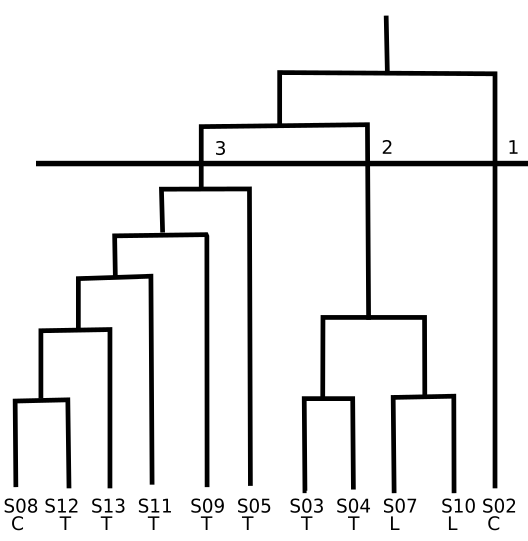
\includegraphics[scale = 0.6]{images/histogramme_sujets_frm}
\caption{Classification tree of manual wheelchair users}
\label{classification_tree}
\end{figure}

These experiments reveal that the subject S02 moves differently from all the other subjects participating in the experiment. Subjects S03, S04, S07 and S10 move similarly, as do subjects S08, S12, S13, S11, S09, and S05.


By crossing this classification with the frequency of appearance of each type of cycle, we observe that only the subject S02 is classified in cluster 1 and it is also the only subject which carries out mainly cycles of type A. The subjects S03, S04, S07 and S10 were classified in cluster 2 and all four carry out majority cycles of type B and C. Subjects S08, S12, S13, S11, S09, and S05 were classified in cluster 3 and these subjects mainly carry out cycles of type A and D. The case of subject S05 is particular, because it also carries out cycles of type B and C, it could thus have been classified in cluster 2. It was finally classified in cluster 3 because of the significant presence of D-type cycles during its movement. The additional information we have on users indicates that the subject S02 is the one with reduced physical abilities. He has been using the Manual Wheelchair once a week for 33 years. This long  experience allowed him to exercise but is not intense enough for significant development of muscle tissue. However, due to its long experience, the subject S02 has a symmetrical propulsion technic. Subjects S03 and S04 both have thoracic lesions, and subjects S07 and S10 both have lumbar lesions. Subject S08 has a low cervical lesion, and subjects S12 and S13 have upper thoracic lesions. 


This information also allows us to deduce that the subjects that are in the same cluster have similar motor abilities, and the subjects belonging to cluster 2 have motor abilities higher than those belonging to cluster 3 who have motor abilities higher than those belonging to cluster 1. We also infer that the majority presence of B and C cycles characterize the movement of subjects with significant motor capacity, that of D-type cycles characterize the movements of subjects with average motor capacity, and that of A-type cycles characterize subjects with weak motor capacity.


We want to establish that the use of the manual wheelchair field-ergometer and the data measured during locomotion in a Manual Wheelchair provides a different but relevant view of locomotion in a Manual Wheelchair. 


Paper \cite{athanasiou2009bayesian} established that the motor abilities of Manual Wheelchair users depend primarily on their level of spinal injury. And this links the physiological characteristics of Wheelchair users and their motor abilities. We consider the physiological characteristics of the subjects who participated in the experiments. These characteristics are Gender, Age, height, weight, dominant limb, level of spinal injury, the severity of injury (complete or incomplete), number of days of practice per week, number of hours of exercise per day. We cross this external information that we have subjects with their motor abilities to determine if this external information would be sufficient to explain the motor abilities of the subjects. We thus obtain the following classification tree using classification algorithm C4.5 (Fig. \ref{physio_tree}): Which suggest that the motor abilities of Manual Wheelchair users depend mainly on the number of practice days per week and also on the level of spinal injury. However, subjects who use the Manual Wheelchair more than one day per week and who have thoracic injuries may have different locomotion abilities that may approach subjects with a cervical injury or subjects with a lumbar injury. This result suggests that the consideration of physiological parameters helps to evaluate the motor abilities of the subjects, but the measurements taken during locomotion allow a more precise evaluation. This experiment highlights a primary interest of the Wheelchair Field Ergometer.

\begin{figure}[h]
\center
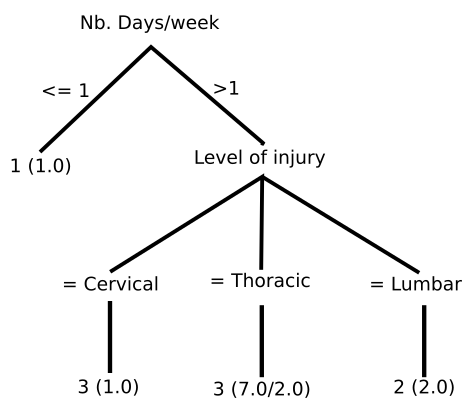
\includegraphics[scale = 0.6]{images/arbre_physio_motor}
\caption{This tree shows that in our experiments, external information only cannot be enough to explain propulsion capabilities of manual wheelchair users}
\label{physio_tree}
\end{figure}


\section{Conclusion}

In this chapter, we have applied the algorithms we have proposed throughout our thesis work to extract time series information from manual wheelchair locomotion. These allowed us to highlight the asymmetrical character of manual wheelchair locomotion, but also to show that manual wheelchair locomotion became more and more symmetrical with years of practice. The experiments also showed that knowledge of the physiological characteristics of subjects in manual wheelchairs was not sufficient for an evaluation of the motor abilities of manual wheelchair users and that an evaluation of locomotion requires measurements to be made in the actual situation of use of the manual wheelchair. The experiments have also shown that the experiment changes the propulsion technology of manual wheelchair users and that these changes vary according to the subjects.


In perspective, we propose to cross the information we obtain from the time series measuring the effort made by the subjects with that representing the kinematics of the body, in particular, the hands of the subjects, and their energy consumption, to evaluate the efficiency of the propulsion techniques in the Manual Wheelchair. Appendix \ref{training_technic} presents a preliminary work on manual wheelchair propulsion technique analysis.


\begin{table}[ht]
\centering
\begin{tabular}{|l|}

\hline
\rowcolor{LavenderBlush}
Key points\\
$\bullet$ We apply the models proposed in Chapters 3, 4 and 5 to cyclical time \\ series from manual wheelchair locomotion. These experiments allow us to \\ highlight the non-symmetrical character of locomotion in a Manual Wheelchair, and also \\ the decrease in the asymmetry of locomotion with years of practice. They also \\ allow us to objectively assess the motor abilities of manual wheelchair users based \\ on cycle properties.\\


 
\hline
\end{tabular}
\end{table}

\chapter*{\textbf{General conclusion and Future works}}
\section*{Aims}
Our primary objective throughout this work was to analyze manual wheelchair locomotion using measurements made by the sensors when using the wheelchair.  This primary objective is divided into three specific goals: how to pre-treat time series to reduce their length and therefore their processing time, how to take into account the existence of uncertainty in the time series during their analysis and finally how to base the exploitation of time series on the cycles that constitute them. Each of these specific objectives has resulted in proposed models.
\section*{Summary of contributions}
\subsection*{Reduce the length of time series with FDTW}
We proposed a heuristic named FDTW that find a suitable parameter to use with the piecewise aggregate approximation algorithm with the aim to reduce the length of time series for classification purpose. This heuristic is based on Greedy Randomized  Adaptative Search Procedure but defines a specific global search strategy. Extensive experimentation has been run out and shows that the compression with FDTW allows reducing the length of time series while keeping their main shape. Moreover, the compression with FDTW can enhance the accuracy of classification because it will enable avoiding pathological alignment with Dynamic Time Warping algorithm this amelioration is particularly perceptible with synthetic datasets.
\subsection*{Dealing with uncertainty using FOTS score}
We introduce a novel dissimilarity score for the comparison of time series named FOTS for Frobenius Correlation for Time series uShapelet discovery. This dissimilarity score is based on local correlation and allows to capture internal properties of the time series while being robust to uncertainty because its computation is based on the comparison of eigenvectors of the autocorrelation matrices of time series. This score has been used for clustering purpose with UShapelet clustering algorithm an shows a significant improvement of the quality of clustering according to the rand Index.
\subsection*{Taking into accounts cycles with a symbolic representation}
Time series coming from wheelchair locomotion are cyclic due to the cyclic aspect of the wheelchair locomotion. The analysis of the wheelchair locomotion is based on those cycles, but none of the data mining models of the literature consider this aspect. We then proposed a symbolic representation of cyclic time series based on the properties of cycles that allow better visualization of the data and a better comprehension of the results obtained after the data mining process. We use this symbolic representation for the analysis of the wheelchair locomotion of eleven users, and this symbolic representation allows establishing that the wheelchair locomotion is asymmetric but this asymmetry get lower and lower with the years' of practice. This symbolic representation also allows a more precise evaluation of motor capabilities of manual wheelchair mainly based on the effort measure during their use of the manual wheelchair.
\section*{Future works and prospects}
\subsection*{Multidimensionality for a better characterization of the propulsion technic}
The analyses in this thesis are based on the Z moment of the wheels of the manual wheelchair. However, several measurements, including seat, back and footrest forces, were taken during the locomotion of the manual wheelchair users. Considering these signals could allow a better analysis of the subjects' movement and therefore suggests that we propose multidimensional data mining models that would simultaneously take into account all the measurements and their characteristics, namely their length, the presence of uncertainty, and the cyclical nature of specific measures.
\subsection*{Fuzziness for a more realistic categorization}
As we saw in Chapter 6 with subject S05, a subject can be very likely to belong to two or more groups. It would, therefore, be wise to associate each assignment with a degree of trust about the subject's group member. This data mining amounts to considering fuzzy approaches in the analysis of time series from manual wheelchair locomotion.
\addcontentsline{toc}{chapter}{Conclusion}
\cleardoublepage% le corps du document est termin�
\pagestyle{back}
\appendix
\chapter[Wheelchair locomotion]{Analysis of manual wheelchair locomotion}
\label{locomotion_analysis}
%\minitoc
\section{Introduction}
Wheelchair locomotion concerns many people, for different reasons: genetic  (myopathy), accidental (spinal cord injury, lower extremity amputee), degenerative (multiple sclerosis, poliomyelitis) or just related to the natural aging of locomotor functions (muscle degeneration, arthritis of the lower limbs, etc.). Then, in the 34 developed countries, it is estimated that 1\% or 10,000,000 people require a wheelchair. In the 156 developing countries, it is estimated that at least 2\% or 121,800,000 people require a wheelchair. Overall, of the 7,091,500,000 people in the world, approximately 131,800,000 or 1.85\% need a wheelchair \cite{Needs2016}. However, the use of manual wheelchair is not without risk.

\section[Problem]{The problem of locomotion manual wheelchair locomotion}
\label{problem}
Although the wheelchair use improves the mobility of its users, doctors quickly realized that it often leads to sedentarization, and to related problems of obesity, diabetes, etc. Also, to promote daily physical activity, sport has been strongly encouraged \cite{machida2013resilience}. However, intensive and prolonged sports practice in Manual WheelChair (MWC) can lead to specific injuries and pains \cite{johnson2004sport}, especially in the shoulder, and at the elbow, wrist and hand. For instance in \cite{pentland1991weight}, the  authors claimed that 73\%  of paraplegic individuals suffered from shoulder pain. In addition, prolonged sitting of   users causes dermatological problems such as bedsores or pressure ulcers, due to immobility, loss of sensitivity and incontinence. These symptoms are recognized as a major cause of discontinuation of wheelchair use \cite{van2006manual}  \cite{ville2006work}, thus the sedentarization of users.  \cite{lundqvist1991spinal} showed that upper limb pain was the main factor correlated with poor quality of life in MWC users. The challenge for the therapist is then to encourage a daily practice of physical activity adapted to  wheelchair users, for limiting orthopedic problems,  and thus to promote the use of the MWC over time.


Given the problems faced by manual wheelchair users at the level of
their autonomy and health, van der Woude et al. \cite{van2005wheelchair} \cite{woude1986wheelchair} summarized the issues of manual wheelchair locomotion research into three main areas:

\begin{itemize}
\item Improving the interface between the subject and his manual wheelchair, that is, the ergonomy and the adequacy of the system \{subject + MWC\} with the external physical environment (ramps, lifts, corridor widths, etc.).
\item The improvement of the MWC regarding the design and the mechanical principles of propulsion;
\item \textbf{Improving the subject's physical abilities}, that is, improving propulsion techniques, as well as rehabilitation techniques and training programs.
\end{itemize}

After the construction of a measuring tool,  a wheelchair field ergometer \ref{dabonneville2005self},  bio-mechanical works has been conducted in LIMOS to identify and quantify traumatic factors such as \cite{Remy2005}  \cite{Sauret2010}. 

\section[Evaluation tools]{Tools to evaluate manual wheelchair locomotion}
\label{measurment_tools}
This section summarises different tools designed over the last 60 years to measure the efforts made by subjects moving in a MWC. We put a  particular emphasis on the wheelchair  ergometer designed and manufactured at LIMOS, which is at the origin of the time series that are the subject of our analysis throughout this thesis.

\subsection{Crank Ergometers}
Crank ergometers allow a subject to manually operate a crankset connected to the flywheel of an ergo-cycle. The speed is determined by measuring the rotation speed of the flywheel, whose diameter is known, or by imposing a cadence, in which case the rotation speed is considered constant. Crank ergometers established that the mechanical work of the upper limbs is less efficient than that of the lower limbs and also that the physical capacities evaluated by the maximum oxygen consumption of MWC users depended on their level of spinal injury (cervical, thoracic or lumbar injury)\footnote{This assertion will be commented later in chapter \ref{chapter_saxp}}. One of the main limitations of crank ergometers is that the motion measured from a crank ergometer is not representative of the MWC propulsion motion, most of which is propelled by handrims \cite{0aastrand1961maximal}  \cite{bergh1976maximal}    \cite{stenberg1967hemodynamic}.

\subsection{Roller Ergometers}
To reproduce more precisely the specificities of  MWC locomotion, Brouha and Krobathc\cite{brouha1967continuous}, as early as 1967, used a roller ergometer to measure cardiac and respiratory responses during continuous MWC exercice. This tool consisted of a platform on which were fixed two rollers, each rotating around an axis and on which rested the rear wheels of a real MWC. The MWC frame was attached to the ergometer, and the subjects simulated locomotion by applying forces to the handrims, causing the rear wheels of the MWC and the rollers to rotate. 


In 1971, Stoboy et al. \cite{stoboy1971workload}, using an ergometer inspired by that of Brouha and Krobath, quantified the mechanical power (in watts) produced by the user from the relationship between oxygen consumption and mechanical power calculated during an incremental exercise on a crank ergometer.


The problem with roller ergometers of \cite{brouha1967continuous}\\\cite{stoboy1971workload} was that they did not take into account the influence of the inertia of translation encountered by the Subject when he moves. To take this phenomenon into account, the rollers have been connected  to a small flywheel. However,  both rear wheels were on the same rollers, which did not allow to measure the differences in propulsion between the right and left wheels to be explored \cite{brouha1967continuous} \cite{stoboy1971workload}.



Then \cite{langbein1993research} \cite{langbein1993calibration} \cite{langbein1994initial}  designed a new roller ergometer called the Wheelchair Aerobic Fitness Trainer (WAFT), which had an access ramp to facilitate subject and MWC installation (Figure \ref{WAFT}). When the latter was attached to the ergometer, its rear wheels rested on three rollers each, which made it possible to differentiate the forces applied to the right and left wheels\footnote{This separation is essential to establish the dissymmetry of wheelchair locomotion and is discussed in more details in chapter \ref{chapter_saxp}}.

\begin{figure}[h]
\center
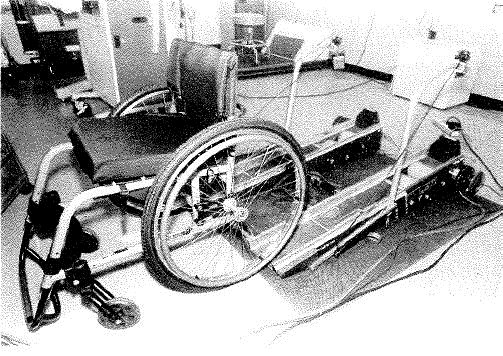
\includegraphics[scale = 25]{images/WAFT}
\caption{ Wheelchair Aerobic Fitness Trainer (WAFT) photograph \cite{langbein1993research}.}
\label{WAFT}
\end{figure}


Other roller ergometers have also been developed over the last four decades and particularly in the last fifteen years: Eagle Wheelchair Roller \cite{kerk1995effect}, Bromking Turbo Trainer \cite{goosey2001kinetic} \cite{goosey2001kinetic} \cite{ price1999thermoregulatory} or very recently the "Computer Monitored Wheelchair Dynamometer" \cite{cooper2003wheelchair}  \cite{digiovine2001dynamic}.  Other braking systems have been used, such as mechanical braking using a friction belt on a flywheel\\\cite{goosey1998relationship}  \cite{kulig2001effect} \cite{rodgers1994biomechanics}(Figure \ref{FRER}), an electric motor creating a frictional moment around the roller rotation axes \\\cite{coutts1987aerobic} \cite{kerk1995effect} \cite{patterson1997selected}     \\ \cite{vanlandewijck1999field} or an isokinetic apparatus  \cite{ruggles1994biomechanics}. To determine the speed, angular position sensors  \cite{brouha1967continuous}  \\ \cite{coutts1987aerobic}  \cite{coutts1990kinematics}  \cite{patterson1997selected} \\ \cite{rodgers1994biomechanics}, optical encoders   \cite{devillard1999wheelchair} \cite{devillard2001validation}   \\ \cite{langbein1993calibration}  \cite{langbein1994initial}  \cite{newsam1996temporal}  \\ \cite{theisen1996new}, tachometers  \cite{cooper1990exploratory}  \cite{kerk1995effect}   \cite{masse1992biomechanical} \\  \cite{vanlandewijck1999field} or speedometers   \cite{goosey1998relationship}  \cite{rodgers1994biomechanics} were used.

\begin{figure}[h]
\center
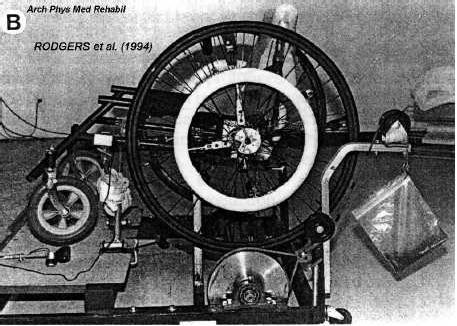
\includegraphics[scale = 25]{images/FRER}
\caption{Picture of a wheelchair on a roller ergometer with mechanical braking by friction belt on a flywheel. \cite{rodgers1994biomechanics}.}
\label{FRER}
\end{figure}

The main advantage of roller ergometers is that they allow subjects to be studied with their own MWC. Moreover, they occupy a little space in the laboratory and allow the MWC to be completely immobilized, thus ensuring the stability of the subject on the MWC and facilitating the measurement of  various physiological parameters. However, the various methods for estimating external  mechanical power used up to now still need to be refined to better evaluate this parameter. Furthermore, the comparison between the results of studies carried out with different roller ergometers and different mechanical models must be done with caution since the parameters neglected or taken into account are not all the same.

\subsection{Treadmill}
Like roller ergometers, the main advantage of treadmills is that they allow subjects to be studied with their own MWC. Since the four wheels of the MWC roll on the belt, the rolling friction forces are most certainly equivalent to those existing on the ground. Unlike roller ergometers, treadmills  allow to define a rolling speed of the belt and also a slope, that is, an inclination of the treadmill with respect to the horizontal. The main disadvantage of a treadmill comes from the steering problem related to the control of the trajectory: indeed, a subject could drift and be ejected from the treadmill; to remedy this, railings have been installed on both sides using a surface strip that limits lateral movements \cite{claremont1985model}. However, it has still not been demonstrated that the propulsion technique used was identical on a treadmill and on the ground.

\begin{figure}[h]
\center
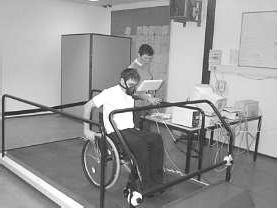
\includegraphics[scale = 40]{images/tapi_roulant}
\caption{ Exercise testing on a motor driven treadmill \cite{van2006manual}}
\label{tapi_roulant}
\end{figure}

\subsection{Wheelchair simulators}
To overcome the problems related to rolling resistance, some researchers chose to fix the rear wheels of the MWC without contact with the ground, on a rigid and fixed chassis on which the Subject could sit. The advantage of MWC simulators is that they can test different settings such as seat position or rear wheel camber angle, for example. The mechanical propulsion model is also simplified compared to roller ergometers and conveyor belts, which allows a better quantification of work and external mechanical power.   However, the influence of the Subject's movements on the seat is not taken into account. This aspect is the major disadvantage of the simulators because neither the forces of resistance to the advance nor the kinematics of the MWC is modified according to the movements of the Subject on the seat.

\begin{figure}[h]
\center
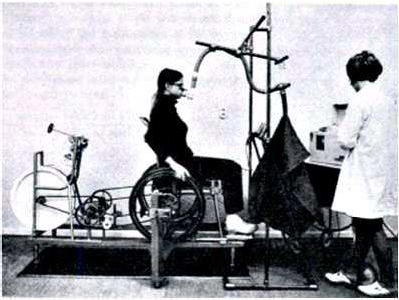
\includegraphics[scale = 30]{images/SFR}
\caption{Photograph of an experiment on a simulator connected to a flywheel (\cite{brattgaard1970energy})}
\label{SFR}
\end{figure}

\subsection{Wheelchair Field-Ergometer}
To analyse the efficiency of wheelchair propulsion, a Wireless Wheelchair Ergometer (WWE or FRET-1)  equipped with several sensors has been manufactured \cite{dabonneville2005self}. The sensors installed on the wheelchair measure the physical stresses applied to the MWC during actual use and record them.


The sensors are located on the right and left wheels of the MWC, on the footrest, on the seat and the backrest. These sensors measure the torques applied to each of the systems mentioned above.  Other sensors installed on the FRET-2 are used to measure the kinematic parameters (speed, acceleration) of the movement of the MWC (Figure \ref{fret_legend}).


\begin{figure}[h]
\center
\includegraphics[scale = 0.4]{images/FRET-2_Legend_GB}
\caption{Captioned picture of the adjustable wireless wheelchair ergometer (FRET-2).}
\label{fret_legend}
\end{figure}


The measurements recorded by the sensors, which are the prupose of our analysis, consist of 41 attributes; of which 30 represent the dynamic parameters (Fx, Fy, Fz, Mx, My, Mz = 6 components x 5 dynamometers). The 11 other attributes represent the kinematic parameters of the MWC and its position relative to the Earth's magnetic North.

\subsubsection{The force and torque dynamometer}

A "torsor" is a mathematical object that characterizes the efforts applied on – or by – a solid. It is composed of two vectors, which have three components each: the three components (Fx, Fy, Fz) of the resulting force (F) and the three components (Mx, My, Mz) of the resulting moment (M) that are applied to this solid along three orthogonal axes (x, y, z). To measure the six components of the "torsor" applied by wheelchair users on both handrims during their actual displacements on the ground, an original force and torque dynamometer has been designed, built and installed on both rear wheels of the FRET-1 and then the FRET-2 (Fig. \ref{capteur_tri_axe}). This dynamometer is composed of three bidirectional force sensors that measure all the forces applied to the handrim which are then used to compute the three components of the resulting force and the three components of the resulting moment.

\begin{figure}[h]
\center
\includegraphics[scale = 0.4]{images/principle_six_component_sensor}
\caption{Schematic principle of the six-component force and torque sensor (patent WO 1995001556 A1) mounted of both rear wheels of the MWC field ergometer used in this study (FRET-2).
\\
\textbf{Legend}
\begin{itemize}
\item $R^{*} (O,\,x,\,y,\,z)$: moving reference frame linked to the wheel;
\item $O:$ centre of the wheelchair rear wheel;
\item $R:$ radius of the wheelchair rear wheel;
\item $A,\, B,\, C:$ locations of the three two-component force tranducers;
\item $u1,\, ... ,\, u6:$ unit vectors of the six force transducers;
\item $F_{ext}$: external force applied by the user on the handrim;
\item $P:$ point of application of Fext on the handrim;
\item Angles: $a = (u_x, F_{ext}); b = (u_z, F_{ext}); q = (u_x, OP)$ 
\end{itemize}
}
\label{capteur_tri_axe}
\end{figure}



The wheel dynamometer used in that study is based on a mechanical principle already applied for the design of a six-component dynamometer used for the measurement of the forces and torques applied by the pole-and-vaulter system in the vaulting box during the pole vault.

According to that principle, the handrim is assumed to be rigid and firmly fixed on three two-component force transducers designed to measure the handrim displacement with respect to the wheel. In that approach, the handrim is considered as hanging on the wheel through the force transducers. Each transducer measures one component of the resulting propulsive force in the tangential direction of the wheel and one in the direction perpendicular to the plane of the wheel. The vectorial sum of all these components is equal to the resulting propulsive force in the moving reference frame $R^{*}$ linked to the wheel. This derives from the fact that the handrim is static in $R^{*}$ with respect to the wheel.


When an external force Fext is applied on the handrim, it is instantaneously transmitted to the six force transducers so that each of them simultaneously measures a local force $F_i$ $(i = 1 \, to \, 6)$. As the transducers behave as springs, which stiffness $k_i$ are determined through the calibration procedure, the measurement of the displacements $m_i$ by the strain gauges allows to compute the values of $F_i$ using Hooke's law (equation \ref{eq:hooke})

\begin{eqnarray}
F_i = k_i m_i.
\label{eq:hooke}
\end{eqnarray}



Finally, the force and torque components created by $F_{ext}$ are calculated by equation \ref{eq:torseur}

\begin{eqnarray}

\overrightarrow{F}_{ext}=
\stackrel[i=1]{6}{\sum}\vec{F}_{i}\iff\left[F_{ext}\right]=
\left[k_{i}\right]\left[m_{i}\right]\iff\left[F_{ext}\right]=\left[\begin{array}{c}
F_{x}\\
F_{y}\\
F_{z}\\
M_{x}\\
M_{y}\\
M_{z}
\end{array}\right]

\label{eq:torseur}

\end{eqnarray}

Where $\left[F_{ext}\right]$ is a column matrix containing the six components of the torsor applied on the dynamometer; $\left[k_{i}\right]$ is the sensitivity matrix of the dynamometer;  $\left[m_{i}\right]$ is the column matrix containing the signals measured by the six forces transducers of the dynamometer.
Several mechanical and kinetic parameters can be computed from the forces and torques measured by the six-component dynamometers mounted on the MWC field ergometer \cite{Sauret2010}. All of them have a specific and useful meaning as their relationships are defined by a complete mechanical (i.e. dynamic and kinematic) model of wheelchair propulsion. However, because of their number and their complexity, these parameters can only be analysed and interpreted by specialists in biomechanics. To overcome this drawback, in the present study, relevant mechanical information has been extracted from only some dynamic data (z-moments $M_z$) recorded by both rear wheel dynamometers of the instrumented MWC (FRET-2) [This information have then been used to group subjects in homogeneous clusters, which have been compared to clinical injury levels.

\section[Wheelchair time series]{Knowledge discovery on wheelchair time series}
\label{mechanical_model}
After the construction of these measuring instruments (FRET-1 and FRET-2), they have been used to measure the efforts made by MWC uses in actual conditions of wheelchair locomotion. Thus, several experiments have been conducted with several subjects,  where the efforts produced during actual wheelchair locomotion were measured with the FRET-2. The abundance of the recorded measurements highlighted the problem of the exploitation of these measures for knowledge extraction. Two main and complementary approaches can be used to analyze measurements from MWC locomotion. The first is to use mechanical models to calculate the physical parameters of motion and the second is to use data mining models to exploit measurements.  In this section, we present the contributions of these two approaches, which will allow us to position our work.



\paragraph{}Manual wheelchair locomotion causes significant mechanical stresses in the upper limbs \cite{desroches2010expression}. To remedy this problem, biomechanical studies have been conducted to identify and quantify traumatic factors such as:
\begin{itemize}
\item The doctoral thesis of Nicolas DE SAINT REMY (2005) \cite{Remy2005} who proposed a
mechanical model relating the forces applied to a MWC and its displacement ( Figure \ref{Wheelchair_model} ). This work particularly highlighted the fact that wheelchair acceleration is a function of subject's movements.

\begin{figure}[h]
\center
\includegraphics[scale = 0.6]{images/wheelchair_model2}
\caption{Balance of forces applied to a manual wheelchair during propulsion. For the clarity of the figure, the analysis of the movement of the {subject + MWC} system is reduced to that of the system's centre of gravity, G \cite{Remy2005}}
\label{Wheelchair_model}
\end{figure}

\item The doctoral thesis of Christophe SAURET (2010) \cite{Sauret2010} who proposed a method of calculating the mechanical power developed by manual wheelchair users to move. This model analyzes the kinetics of the \{subject + MWC\} system. For that purpose, the author developped a detailed kinematic model of the \{subject + MWC\} system (Figure \ref{Wheelchair_model2}) allowing to record their movements with a 3D motion analysis system during actual locomotion on the ground. 


\begin{figure}[h]
\center
\includegraphics[scale = 0.5]{images/squelette}
\caption{Locations of passive markers for the kinematic analysis of manual wheelchair locomotion \cite{Sauret2010}}
\label{Wheelchair_model2}
\end{figure}

\end{itemize}


\paragraph{} More and more works in the literature suggest using the tools developed in data mining for a better understanding of human locomotion. For example, in \cite{van2017future}, the authors ask whether advances in data science and technology could provide a different and perhaps more objective view of the analysis of wheelchair users' motor abilities. On one hand, technical advances have made it possible to measure the efforts made by wheelchair users during their movement using sensors. On the other hand, datamining models have been proposed and allow to perform several task on the data (clustering, classification, …). 

In \cite{faria2012patient} the authors explained how they used robotics and data mining knowledge to build an Intelligent Manual Wheelchair, which can be controlled from multiple interfaces: joysticks, facial expressions, voice commands, head movements.  Since Intelligent Wheelchair users have various characteristics, a series of tests have been carried out to classify them and to define profiles that allow the MWC to be appropriately adjusted  for each user.

In \cite{athanasiou2009bayesian} the authors presented a model based on Bayesian networks to improve the medical treatment of patients in wheelchairs with a spinal cord injury. Indeed, the treatment of these patients  is based on the level of spinal cord injury and symptoms. A lesion in the spine has three consequences: an inconsistency of the bowel, an inconsistency of the bladder, a loss of the skin sensitivity. The higher the lesion, the more widespread its effects on patients are. Thus a patient with a low lesion will affect the patient's legs  and a patient with a high lesion will see his four limbs affected. Because of this loss of sensitivity, symptoms observed in the patient are often incomplete, which introduces uncertainty into the diagnosis that is captured by Bayesian networks and conditional probabilities.





\section{Conclusion}



Throughout this chapter, we showed that there is a large number of MWC users in the world and that it is crucial to analyze this particular means of locomotion to improve the living conditions of people moving in a MWC. We have presented the main tools designed and manufactured for wheelchair locomotion analysis and some previous works that used data mining mechanics models to improve the study of wheelchair locomotion or  to  help physicians to diagnose its the adverse effects. 


In the scientific literature,  mechanical or data mining models are used for manual wheelchair locomotion analysis.  In this thesis, however, we want to \textbf{design} data mining models that are able to take into account both the specificities of MWC locomotion data and their use to analyze wheelchair locomotion from a new point of view. 


%\chapter{Hellinger Based Distance for Uncertain time series}
%\label{helinger}
%Deterministic Measures like traditional similarity measures, return a real number as
%the distance between two uncertain time series. 







































\chapter{An optimal approach for time series segmentation: Application to the supervised classification}
\label{seg}

\section{Introduction}
Time series databases are often huge. This is particularly the case of the Large Synoptic Survey Telescope (LSST) database which records data from of telescopes \cite {lsst}. It has billions of time series (10 Petabytes). The time series recorded in these databases are sometimes very long. Another example is the  SACR-FRM project that uses sensors to measure the efforts of a  manual wheelchair user at a frequency of 100 Hz \cite{SACR-FRM}. Ten minutes recording time series of 60 000 measurements. Faced with this, several scientific works were carried out with the aim of reducing the storage space of time series and accelerating their treatment.  A widely used approach is to change the representation of time series to reduce their length. This technique was introduced by Agrawal et al. \cite{Agrawal1993}; he uses the discrete Fourier transform to obtain a compact representation of the time series.
 Other methods have also been used: the decomposition in eigenvalue \cite{Wu1996}, the  discrete wavelet transform \cite{Chan1999} and the piecewise approximate aggregation (PAA) \cite{keogh2001locally}. This last method has shown its effectiveness compared to previous three because it is easier to understand, to implement, but also faster and allows to build indexes in linear time. PAA suggests splitting the time series into segments of the same length, then replace each segment by the average of its points. This method generates a compact representation, able to have a few segments as possible to reduce space storage and processing time of time series.
 However, a too compact representation distorts the time series and causes a loss of information. How then to choose the right number of segments to consider? Our work is based on a simple observation: the use of the arithmetic average is relevant when the variance of the population is small as illustrated by the figure \ref{fig:average}.
 
 

\begin{figure}
\centering
\subfloat[]{\includegraphics[scale=0.6]{moyenne_des_segment1.jpg}} \subfloat[]{\includegraphics[scale=0.6]{moyenne_des_segment2.jpg}}
\caption{These figures show the average of two segments. In the first
case (a) the data points of the segment are far from the average, in the second case (b) they are close to the average. Replace data points of a segment by their average introduces an error that the can be measured from the gap between the points and the average. }

\label{fig:average}
\end{figure}


 
 
 We define here a minimal bound for the number of segments to be considered, and we propose an algorithm which allows choosing the number of segments which minimizes their mean squared error, with the aim to reduce the length of the time series without altering the information they contain.
 
 
  The rest of this chapter is organized as follows: the \ref{problem} section presents a formal definition of our problem and an algorithm used to solve it; the section \ref{results} presents and comments the results of the experiments and the section \ref{conclusion} concludes the paper and presents perspectives for this work.
 

\section{Granularity of time series segments}
\label{probleme}


\subsection{Notations and definitions}
\paragraph{Definition 1:} A \textbf{time series} or \textbf{time series}
$ X = x_{0}, x_{1}, \cdots, x_{m} $ is a sequence of numerical values representing the evolution of a specific quantity over time. $ x_{m} $ is the most recent value.

\paragraph{Definition 2:} A segment $ X_{i} $ of length $ l $ of the time series
$ X $ of size $ m $ $ (l <m) $ is a sequence consisting of $ l $ consecutive variables
$ X $ beginning at the  position  $ i $  and ending at the position $ i + l-1 $.
We have: $ X_{i} = x_{i}, x_{i + 1}, ..., x_{i + l-1} $

\paragraph{Definition 3:} The arithmetic mean of the data points of a segment $ X_{i} $ of size $ l $ is
denoted $ \bar {X}_{i} $ and is defined by
\[
\bar{X}_{i} = \frac{1}{l} \sum_{j = 0}^{l-1} x_{i + j}.
\]



\subsection{Information theory and minimum number of segments}
To mitigate the effects of noise during time series processing, Keogh and Kasetty \cite{KeoghBenchmarks} recommend that they are normalized. Normalizing the time series makes them compatible with a normal distribution \cite{Lin2007}. In this case, 95 \% of the points in the time series are between minus two times the standard deviation $ (\sigma) $ and twice the standard deviation of the points, and thus 5 \% of the points of the series are outside this range. These points correspond to the ends of the series as shown in the figure \ref{standard_deviation}.


\begin{figure}
\centering
\includegraphics[scale = 0.50]{fordA_ecart-type}
\caption{This figure shows the first 100 points of the first time series  of the fordA dataset available in the UCR \cite{UCRArchive} database. Time series are normalized. The two horizontal lines delimit the interval corresponding to twice the standard deviation and minus two times the standard deviation of the points of the time series. We can observe that the points outside this range are at the ends of the time series.}
\label{standard_deviation} 
\end{figure}



\subsection{Notations and definitions}
\paragraph{Definition 1:} A \textbf{time series} or \textbf{time series}
$ X = x_{0}, x_{1}, \cdots, x_{m} $ is a sequence of numerical values representing the evolution of a specific quantity over time. $ x_{m} $ is the most recent value.

\paragraph{Definition 2:} A segment $ X_{i} $ of length $ l $ of the time series
$ X $ of size $ m $ $ (l <m) $ is a sequence consisting of $ l $ consecutive variables
$ X $ beginning at the  position  $ i $  and ending at the position $ i + l-1 $.
We have: $ X_{i} = x_{i}, x_{i + 1}, ..., x_{i + l-1} $

\paragraph{Definition 3:} The arithmetic mean of the data points of a segment $ X_{i} $ of size $ l $ is
denoted $ \bar {X}_{i} $ and is defined by
\[
\bar{X}_{i} = \frac{1}{l} \sum_{j = 0}^{l-1} x_{i + j}.
\]




Also, information theory tells us that the amount of information relating to an event is equal to $ -log_{2}(p) $ where $ p $ is the probability of the event
\cite{Shannon2001} . In other words, a very likely event ($ p \longrightarrow1 $) brings less information than an unlikely event ($ p \longrightarrow0 $). Therefore, a point outside the interval $ [- 2 \sigma, 2 \sigma] $ provides more information than a point in that range. Indeed, the probability that one point is in the range is $ 0.95$ while the probability that one point is out of range is $ 0.05 = \frac{1}{20} $ .


If we choose a minimum number $ (\alpha) $ of segments less than 5 \% of the length of the time series, we risk to aggregate the data points within the interval $ [- 2 \sigma, 2 \sigma] $ and those outside this range. This will have two consequences: firstly, this aggregation will alter the information carried by data points. Secondly, this aggregation will increase the variance of the segments obtained. So we chose to  consider 5\% of the number of points in the time series as the minimum number of segments. This allows us to define the following functions of $ \mathbb{N} \rightarrow \mathbb{N} $:

\[
\alpha: n \mapsto \alpha(n) = \left \{
\begin{array}{c}
\left \lfloor \frac{n}{20} \right \rfloor \: if \: \left \lfloor \frac{n}{20} \right \rfloor \geq 2 \\
2 \: otherwise
\end{array} 
\right.
\]



\[
\beta: n \mapsto \beta(n) = \left \lfloor \frac{n}{2} \right \rfloor
\]
 $ \beta $ gives the maximum number of segments. Indeed, a segment is made up of at least 2 points, so there is at most $ \left \lfloor
\frac{n}{2} \right \rfloor $ segments. The number of segments W that we will consider is greater than or equal to $ \alpha (| X |) $ and less than or equal to $ \beta (| X |) $. The next subsection explains how we choose the value of W.

\subsection{Minimize the squared error to choose the number of segments}
After dividing into segments, we replace each segment by the average of the data points that constitute it. The variance between the points of each segment can be measured from the mean squared error. Our problem is therefore the following:
\paragraph{} Let $ X = x_{0}, x_{1}, \cdots, x_{n} $ a time series of size $ n $, look for $ W \in \mathbb{N} $ such that $ \alpha(n) \leq W \leq \beta(n) $ and $ \frac{1}{n} \sum_{i = 1}^{^{W}} \sum_{j = (i-1) k}^{ik} (\bar{X}_{i} - X_{j})^{2} $ is minimal. Where $ \bar{X}_{i} $ is the arithmetic mean of a segment of length $ k $. 




\paragraph{} To solve this problem, we
propose an algorithm that proceeds as follows:
\begin{enumerate}
\item For each value of W, with $ \alpha(n) \leq W \leq \beta(n) $
\begin{enumerate}
\item Calculate the squared error of each segment
$ X_{i} = x_{i}, x_{i + 1}, ..., x_{i + l-1}; $
\item Calculate the mean of the quadratic errors;
\end{enumerate}
\item The value of W returned is the one that produces a minimum average squared error; 
\end{enumerate}

Algorithm \ref{algo1} details the previous principle.


\begin{algorithm}[h]
\DontPrintSemicolon
\KwIn{length\_min, length\_max : repectively the minimal and the maximal length of a segment.\\ v : a time series}
\KwOut{The optimal number of segment to be use with Piecewise Aggregate approXimation}
\SetKwBlock{Begin}{function}{end function}

\Begin($\text{optimalNumberOfSegment} {(} length\_min, \, length\_max, \, v{)}$)
{
  $len\_v \leftarrow length(v)$\;
  $n \leftarrow length\_max - length\_min + 1$\;
  \ForAll{$i \in \{length\_min,...,length\_max\}$}
  {
    $x[j, 1] \leftarrow i$\;
    $z[j, 1] \leftarrow  (1/len\_v) * sum\_SSE(v, i)$\; \\computation of the error    
		$j \leftarrow j + 1$\;
  }
	$ind\_min \leftarrow indice\_minimun(z)$\;
  \Return{$floor(len\_v/x[ind\_min, 1])$}

}
\caption{optimalNumberOfSegment}
\label{algo1}
\end{algorithm}


%\begin{algorithm}
%\caption{longueur\_optimale (long\_min, long\_max, v)}
%\begin{algorithmic} 
%\STATE $len\_v \leftarrow length(v)$
%\STATE $n \leftarrow long\_max - long\_min + 1$
%\FOR{$(i\, in \,long\_min:long\_max)$} 
% \STATE $x[j, 1] \leftarrow i$
% \STATE $z[j, 1] \leftarrow  (1/len\_v) * somme\_SSE(v, i)$ //Calcul de l'erreur
% \STATE $j \leftarrow j + 1$
%%\ENDFOR
% \STATE $ind\_min \leftarrow indice\_minimun(z)$
%\RETURN $floor(len\_v/x[ind\_min, 1])$
%\end{algorithmic}
%\end{algorithm}


%\begin{algorithm}
%\caption{sum\_SSE (v, nbPoints)}
%\begin{algorithmic} 
%\STATE $n \leftarrow length(v)$
%\STATE $ind\_debut \leftarrow 1$
%\STATE $aux\_se \leftarrow c()$
%\STATE $tableau\_indice\_debut \leftarrow c()$
%\STATE $i \leftarrow 0$

%\WHILE{$(ind\_debut + nbPoints) \leq n$} 
%\STATE $tableau\_indice\_debut[i] \leftarrow ind\_debut$
%\STATE $ind\_debut \leftarrow ind\_debut + nbPoints$
%\STATE $i \leftarrow i + 1$
%\ENDWHILE

%\STATE $m \leftarrow length(tableau\_indice\_debut)$
%%\FOR{(i in 1:m) parallel loop} 
% \STATE $aux\_se[i] \leftarrow $
%\STATE$ SSE\_segment(v, nbPoints, tableau\_indice\_debut[i])$
%\ENDFOR
%\RETURN $somme(aux\_se)$
%\end{algorithmic}
%\end{algorithm}

\begin{algorithm}[h]
\DontPrintSemicolon
\KwIn{v : a time series.\\ nbPoints : the length of a segment}
\KwOut{The sum of squares error associated with a segment length}
\SetKwBlock{Begin}{function}{end function}

\Begin($\text{sum\_SSE} {(} v, \, nbPoints{)}$)
{
  $n \leftarrow length(v)$\;
	$ind\_debut \leftarrow 1$\;
	$aux\_se \leftarrow c()$\;
	$tab\_indices\_debut \leftarrow c()$\;
	$i \leftarrow 0$\;
	
	\While{$(ind\_debut + nbPoints) \leq n$}
	{
		$tab\_indices\_debut[i] \leftarrow ind\_debut$\;
		$ind\_debut \leftarrow ind\_debut + nbPoints$\;
		$i \leftarrow i + 1$\;
	}
	
	$m \leftarrow length(tab\_indices\_debut)$\;
	
	 \ForAll{$i \in \{1,...,m\}$}
  {
		$aux\_se[i] \leftarrow SSE\_segment(v, nbPoints, tab\_indices\_debut[i]) $\;
  }

  \Return{$sum(aux\_se)$}

}
\caption{sum\_SSE}
\label{algo2}
\end{algorithm}
 
 

\paragraph{Complexity of the algorithm}
The calculation of the squared error of a segment is done in $ O(\left \lfloor
\frac{n}{W} \right \rfloor) $.

The time complexity of calculating the mean squared error for segment splitting is
$ O(n). $


The number of segments varies from $ \left \lfloor \frac{n}{20} \right \rfloor, \; \left \lfloor \frac{n}{19} \right \rfloor $ \ldots $ \left \lfloor \frac{n}{2} \right \rfloor $. There are 19 possible divisions in segments. The time complexity of calculating the value of W which minimizes the error
mean squared is $ 19 \times O(n) = O(n) $.


To exploit the compact representations of the time series, we must be able to compare them. The next subsection presents how to compare compact time series that we get.

\subsection{Dynamic Time Warping Algorithm and comparison of compact representations}

The dynamic time warping algorithm \cite{Keogh2004} allows to carry out a non-linear correspondence between two time series by minimizing the distance between the two. It proceeds as follows:
Let $X$ and $Y$ be two time series;

\[
X=x_{1},x_{2},\cdots,x_{n};
\]


\[
Y=y_{1},y_{2},\cdots,y_{m}.
\]

 To align them, the algorithm constructs a matrix $ n \times m $ where
the element $ (i, j) $ of the matrix corresponds to the square distance $ (x_{i} - y_{j}) ^ {2} $ which
is the alignment between $ x_{i} $ and $ y_{j} $. To find the best alignment between the two time series, we build
the path in the matrix that minimizes the sum of the square distances. This path is calculated by
dynamic programming from the following recurrence:
\[
\gamma(i, j) = d (x_{i}, y_{j}) + min \{\gamma(i-1, j-1), \gamma(i-1, j), \gamma(i , j-1) \},
\]
where $ d(x_{i}, y_{j}) $ is the square of the distance contained in the cell $ (i, j) $ and $ \gamma(i, j) $ is the
cumulative distance at the position $ (i, j) $ which is calculated by the sum of the square of the distance to
the position $ (i, j) $ and the minimum cumulative distance of its three adjacent cells.


Piecewise aggregate approximation provides Euclidean-based distance measurement to compare compact representations. However, we chose to use the dynamic time warping algorithm. For the following reasons:
\begin{enumerate}
\item The dynamic time warping algorithm  is known to have the best performance for sequence alignment in several areas:
in robotics, biometrics, music, climatology, aviation, in gesture recognition, cryptanalysis, astronomy, exploration
space \cite{Rakthanmanon2012}.
\item Piecewise aggregate approximation of the time series leads to temporal deformation. Indeed,
with two time series of length $ n $, we can apply our algorithm to the
 first time series, then reduce it to $ N_{1} $ segments and reduce the second to $ N_{2} $
 segments with $ N_{1} <N_{2} $.
\end{enumerate}


\section{Results and Discussion}
\label{results} 
 First, we present the datasets used during the experiment.
 Then we evaluate the performances of the proposed methods in terms of  reduction of the
 length of time series and classification errors.

\subsection{Datasets}

We performed tests on 85 datasets that come from the UCR database
\cite{UCRArchive} . Detailed information on the datasets is presented in
the table \ref{sets_of_data}.
 In the UCR database, each data set is divided into a learning set and a test set. Datasets contain between 2 and 60 classes and the time series of these datasets have lengths that range from 24 to 2709 points. The table \ref{sets_of_data} presents a
 detailed description of the datasets. The following paragraph presents the assessment of the performance of our algorithm on these datasets.
 
\LTcapwidth=\textwidth
\begin{longtable}
   {|p{0.05\linewidth}|p{0.4\linewidth}|p{0.1\linewidth}|p{0.15\linewidth}|p{0.15\linewidth}|}
   \hline
	 \textbf{N} & \textbf{Name} &\textbf{Nb. of classes} &\textbf{Size of training set} &\textbf{Size of testing set}  \endfirsthead
   \hline
   \textbf{N} & \textbf{Name} &\textbf{Nb. of classes} &\textbf{Size of training set} &\textbf{Size of testing set}  \\
	 \hline
   \multicolumn{5}{|p{0.6666\linewidth}|}{Following ... } \\
   \hline
	 \endhead
   \hline
   \multicolumn{5}{|p{0.6666\linewidth}|}{Continue to the next page}\\ 
	 \hline 
	 \endfoot 
	 \hline
   \multicolumn{5}{|p{0.6666\linewidth}|}{End} \\
   \hline
   \endlastfoot 
	\hline
	
1 & 50Words  & 50  & 450  & 455 \\

2 & Adiac  & 37 & 390 & 391 \\

3 & ArrowHead  & 3 & 36 & 175\\

4 & Beef  & 5 & 30 & 30\\

5 & BeetleFly  & 2  & 20  & 20\\

6 & BirdChicken  & 2  & 20  & 20\\

7 & Car  & 4  & 60  & 60\\

8 & CBF & 3 & 30 & 900\\

9 & ChlorineConcentration  & 3  & 467  & 3840\\
 
10 & CinC\_ECG\_torso  & 4  & 40  & 1380\\

11 & Coffee  & 2  & 28  & 28 \\

12 & Computers  & 2  & 250  & 250\\

13 & Cricket\_X  & 12  & 390  & 390\\

14 & Cricket\_Y  & 12  & 390  & 390\\

15 & Cricket\_Z  & 12  & 390  & 390\\

16 & DiatomSizeReduction  & 4  & 16  & 306\\

17 & DistalPhalanxOutlineAgeGroup  & 3  & 139  & 400\\
 %& OutlineAgeGroup &  &  & \\

18 & DistalPhalanxOutlineCorrect & 2  & 276  & 600\\
 %& OutlineCorrect  &  &  & \\
 
19 & DistalPhalanxTW  & 6  & 139  & 400 \\

20 & Earthquakes  & 2  & 139 & 322 \\

21 & ECG & 2  & 100  & 100 \\

22 & ECG5000  & 5  & 500 & 4500\\

23 & ECGFiveDays & 2  & 23 & 861\\
24 & ElectricDevices  & 7  & 8926  & 7711\\

25 & Face (all)  & 14  & 560 1 & 690\\

26 & Face (four)  & 4  & 24  & 88\\
 
27 & FacesUCR  & 14  & 200  & 2050\\

28 & Fish & 7  & 175 & 175 \\

29 & FordA  & 2  & 1320 & 3601\\

30 & FordB  & 2  & 810  & 3636 \\

31 & Gun-Point  & 2  & 50  & 150 \\
 
32 & Ham  & 2  & 109 & 105\\
 
33 & HandOutlines  & 2  & 370 & 1000 \\
 
34 & Haptics  & 5  & 155  & 308 \\
 
35 & Herring  & 2 & 64 & 64 \\
 
36 & InlineSkate  & 7  & 100  & 550 \\

37 & InsectWingbeatSound  & 11  & 220  & 1980\\
 
38 & ItalyPowerDemand  & 2  & 67  & 1029 \\
 
39 & LargeKitchenAppliances  & 3  & 375  & 375 \\

40 & Lightning-2  & 2 & 60  & 61 \\
41 & Lightning-7  & 7  & 70  & 73 \\
 
42 & MALLAT & 8  & 55  & 2345\\
 
43 & Meat  & 3 & 60  & 60 \\
 
44 & MedicalImages  & 10  & 381  & 760\\

45 & MiddlePhalanxOutlineAgeGroup & 3  & 154  & 400 \\
 %& OutlineAgeGroup  &  &  & \\
 \ldots& \ldots  & \ldots & \ldots & \ldots \\
\caption{85 UCR  datasets used for experimental validation.
The full list is available here \cite{UCRArchive}}
\label{sets_of_data}
\end{longtable}



\subsection{Comparison of algorithm performance}
% Visionner le code LaTeX du paragraphe 21
The table \ref{erreur_classification} presents the comparison
of the classification error of 1-Nearest Neighbor (1-NN) algorithms associated with Euclidean  distance (4), 1-NN, associated with the dynamic time warping algorithm using a constraint (a deformation window) (5), 1-NN associated with the algorithm of unconstrained dynamic time warping (DTW) applied to the raw data (6) and the 1-NN algorithm associated with DTW applied to the data pre-processed by our algorithm  (7). The $ (4) $ algorithm gives the best results that are to say
$ ((4) \leq (5) \: and \:(4) \leq (6) \: and \:(4) \leq (7)) $ on $ 20 $ datasets, the algorithm $ (5) $ is the best on $ 47 $ datasets, the $ (6) $ algorithm is the best on $ 21 $ datasets, the $ (7) $ algorithm is the best on $ 21 $ datasets. Although no of these algorithms have the best performance on all datasets, the algorithm $ (5) $ averaged the smallest misclassification \textbf{0.237} and the most expensive $ (4) $ algorithm large average error \textbf{0,288}.
The $ (6) $ and $ (7) $ algorithms have relatively close average error rates  equal to \textbf{0,256} and \textbf{0,258} respectively.


To evaluate the effects of the \textbf{change of representation} of the time series on their
\textbf{classification}, we compare the length of the time series and the errors of
classification presented by the columns $ (6) $ and $ (7) $ of the table  \ref{erreur_classification}.
Indeed, these two columns use the same 1-NN classification algorithm and the same function
distance DTW. The only difference between these columns is the nature of the data; the $ (6) $ column
uses the raw data and the column $ (7) $ the compacted data with the method described above.

\begin{itemize}
\item Regarding the length of the time series; the $ (6) $ algorithm uses all the points of
the time series. On the other hand, the $ (7) $ algorithm uses compact representations whose
length varies between \textbf{15} \% and \textbf{34} \% of the initial length of the time series.
On average, the compact representations have a length equal to \textbf {20} \% of the initial time series
\item For classification errors, the error $ (7)> (6) $ on 40 datasets,
the error of $ (7) = (6) $ on 3 datasets and the error of $ (7) <(6) $ on 42 datasets.
\end {itemize}

 These results are encouraging because despite the reduction in the length of the time series
 errors, the classification error with the compact representation is less than or equal to
that of the raw data classification for 45 datasets out of the 85 available in the
UCR base. These results are summarized in Figure \ref{synthesis}. One of the reasons for this observed improvement over 42 datasets is as follows: the dynamic time warping algorithm  is sensitive to noise, therefore by aggregating the points of the segments, we reduce the effects of noise.


% Visionner le code LaTeX du paragraphe 29

\begin{figure}
\center
\subfloat[]{\includegraphics[scale=0.50]{erreur_dtw-reduit_euclid2.png} }
\subfloat[]{\includegraphics[scale=0.50]{erreur_dtw-reduit_dtw(r)2.png}}\\
\subfloat[]{\includegraphics[scale=0.50]{erreur_dtw-reduit_dtw2.png}}

\caption{Two-to-two comparison of the classification errors of the algorithm
1-Nearest Neighbor (1-NN) using Euclidean distance with 1-NN using two variations of the temporal warping algorithm on data
raw and compact data}

\label{synthesis}

\end{figure}



\begin{longtable}
   {|p{0.05\linewidth}|p{0.1\linewidth}|p{0.1\linewidth}|p{0.1\linewidth}|p{0.15\linewidth}|p{0.1\linewidth}|p{0.1\linewidth}|}
   \hline
	 \textbf{(1)} &\textbf{(2)} &\textbf{(3)} &\textbf{(4)} &\textbf{(5)} &\textbf{(6)} &\textbf{(7)} \endfirsthead
   \hline
   \textbf{(1)} &\textbf{(2)} &\textbf{(3)} &\textbf{(4)} &\textbf{(5)} &\textbf{(6)} &\textbf{(7)} \\
	 \hline
   \multicolumn{7}{|p{0.6666\linewidth}|}{Following ... } \\
   \hline
	 \endhead
   \hline
   \multicolumn{7}{|p{0.6666\linewidth}|}{Continue to the next page}\\ 
	 \hline 
	 \endfoot 
	 \hline
   \multicolumn{7}{|p{0.6666\linewidth}|}{End} \\
   \hline
   \endlastfoot 
	\hline
	
1  & 54  & 0,20  & 0,369   & 0,242 (6)  & 0,31  & \textbf{\emph{0,279}}\\
2  & 35  & 0,20  & \emph{0,389 } & 0,391 (3)  & \textbf{0,396 } & 0,425\\
3  & 50  & 0,20  & \emph{0,2 } & \emph{0,200 (0) } & 0,297  & \textbf{0,246}\\
4  & 78  & 0,17  & \emph{0,333} & \emph{0,333 (0) } & \textbf{0,367 } & 0,433\\
5  & 85  & 0,17  & \emph{0,25 } & 0,300 (7)  & 0,3  & \textbf{0,300}\\
6  & 85  & 0,17  & 0,45  & 0,300(6)  & \emph{0,25 } & \textbf{\emph{0,250}}\\
7  & 96  & 0,17 & 0,267  & 0,233 (1)  & 0,267  & \textbf{\emph{0,217}}\\
8  & 32  & 0,25  & 0,148   & 0,004 (11)  & 0,003  & \textbf{\emph{0,002}}\\
9  & 33  & 0,20 & \emph{0,35 } & \emph{0,35 (0) } & \textbf{0,352 } & 0,414\\
10  & 234  & 0,14  & 0,103  & \emph{0,07 (1)}  & 0,349  & \textbf{0,285}\\
11  & 57  & 0,20  & \emph{0 } & \emph{0,000 (0)} & \textbf{\emph{0 }} & 0,036\\
12  & 120  & 0,17  & 0,424  & 0,380 (13)  & \textbf{\emph{0,3 }} & 0,416\\
13  & 60  & 0,20  & 0,423  & 0,228 (10)  & 0,246  & \textbf{\emph{0,241}}\\
14  & 60  & 0,20  & 0,433  & \emph{0,238 (17) } & \textbf{0,256}  & 0,277\\
15 & 60  & 0,20  & 0,413  & 0,254 (5)  & 0,246  & \textbf{\emph{0,244}}\\
16  & 69  & 0,20  & 0,065  & 0,065 (0)  & \textbf{\emph{0,033}} & 0,072\\
17  & 20  & 0,25  & 0,218  & 0,228 (1)  & 0,208  & \textbf{\emph{0,198}}\\
18  & 20  & 0,25  & 0,248  & \emph{0,232 (2) } & \textbf{\emph{0,232}}\emph{ } & 0,255\\
19  & 20  & 0,25  & 0,273  & \emph{0,272 (0) } & \textbf{0,29 } & 0,310\\
20  & 85  & 0,17  & 0,326  & \emph{0,258 (22) } & \textbf{\emph{0,258 }} & 0,276\\
21  & 24  & 0,25  & \emph{0,12 } & \emph{0,120 (0)} & 0,23  & \textbf{0,180}\\
22  & 35  & 0,25  & 0,075  & 0,075 (1)  & 0,076  & \textbf{\emph{0,072}}\\
23  & 34  & 0,25  & \emph{0,203 } & \emph{0,203 (0) } & \textbf{0,232 } & 0,259\\
24  & 24  & 0,25  & 0,45  & \emph{0,376 (14)}  & \textbf{0,399 } & 0,438\\
25  & 32  & 0,24  & 0,286   & \emph{0,192 (3) } & \textbf{\emph{0,192}} & 0,253\\
26  & 70  & 0,20  & 0,216   & \emph{0,114 (2)}  & 0,17  & \textbf{0,170}\\
27  & 32  & 0,24  & 0,231  & \emph{0,088 (12)}  & \textbf{0,095 } & 0,177\\
28  & 77  & 0,17  & 0,217  & \emph{0,154(4) } & \textbf{0,177}  & 0,263\\
29  & 83  & 0,17  & \emph{0,341 } & \emph{0,341 (0)} & 0,438  & \textbf{0,359}\\
30  & 83  & 0,17  & 0,442  & 0,414 (1) & 0,406  & \textbf{\emph{0,360}}\\
31  & 30  & 0,20  & 0,087   & 0,087 (0)  & 0,093 & \textbf{\emph{0,047}}\\
32  & 71  & 0,16  & \emph{0,4 } & \emph{0,400 (0) } & 0,533 & \textbf{0,419}\\
33  & 387  & 0,14 & 0,199  & \emph{0,197 (1) } & \textbf{0,202 } & 0,206\\
34  & 182  & 0,17  & 0,63 & \emph{0,588 (2)}  & 0,623  & \textbf{0,623}\\
35  & 85  & 0,17  & 0,484  & \emph{0,469 (5) } & \textbf{\emph{0,469 }} & 0,500\\
36  & 268  & 0,14 & 0,658 & \emph{0,613 (14)}  &  0,616 & \textbf{0,615}\\
37  & 51  & 0,20  & 0,438  & \emph{0,422 (2) } & 0,645 & \textbf{0,611}\\
38  & 8  & 0,33 & \emph{0,045} & \emph{0,045 (0)} & 0,05  & \textbf{0,048}\\
39  & 120  & 0,17 & 0,507 & 0,205 (94) & 0,205 & \textbf{\emph{0,203}}\\
40 & 106 & 0,17  & 0,246 & \emph{ 0,131 (6)} & \textbf{\emph{0,131}} & 0,164 \\
41 & 63  & 0,20 & 0,425  &  0,288 (5) & 0,274  & \textbf{\emph{0,219}}\\
42  & 170 & 0,17 & 0,086 & 0,086 (0) & \textbf{\emph{0,066}} & 0,097\\
43  & 74 & 0,17 & \emph{0,067 } & \emph{0,067 } & \emph{(0) 0,067} & \textbf{\emph{0,067}}\\
44  & 24 & 0,24  & 0,316  & \emph{0,253 (20)} & \textbf{0,263 } & 0,288\\
45  & 20  & 0,25  & 0,26  & 0,253 (5)  & \textbf{\emph{0,25}} & 0,268\\
46 & 20  & 0,25 & \emph{0,247}  & 0,318 (1) & 0,352  & \textbf{0,268}\\
47  & 20 & 0,25 & 0,439  & 0,419 (2)  & \textbf{\emph{0,416 }} & 0,419\\
48  & 21  & 0,25 & \emph{0,121} & 0,134 (1)  & 0,165  & \textbf{0,133}\\
49  & 125  & 0,17  & \emph{0,171} & 0,185 (1)  & \textbf{0,209} & 0,222 \\
50  & 125 & 0,17  & \emph{0,12 } & 0,129 (1) & \textbf{0,135} & 0,146\\
51  & 95  & 0,17 & \emph{0,133 } & \emph{0,133 (0) } & 0,167  & \textbf{0,167}\\
52  & 71  & 0,17 & 0,479   & 0,388 (7)  & 0,409  & \textbf{\emph{0,355}}\\
53  & 20  & 0,25 & \emph{0,239 } & \emph{0,239 (0) } & \textbf{0,272}  & 0,273\\
54  & 170  & 0,17  & 0,891  & 0,773 (14)  & \textbf{\emph{0,772 }} & 0,809\\
55  & 36  & 0,25  & 0,038 & \emph{0,000 (6)} & \emph{0 } & \textbf{\emph{0,000}}\\
56  & 20  & 0,25  & 0,215 & 0,215 (0)  & \textbf{\emph{0,195 }} & 0,249\\
57  & 20 & 0,25  & \emph{0,192} & 0,210 (1) & \textbf{0,216 } & 0,251\\
58  & 20  & 0,25  & 0,292 & \emph{0,263 (6) } & \textbf{\emph{0,263}} & 0,280\\
59  & 120  & 0,17  & 0,605 & 0,560 (8)  & 0,536 & \textbf{\emph{0,501}}\\
60  & 120  & 0,17  & 0,64  & \emph{0,589 (17) } & \textbf{0,603 } & 0,645\\
61  & 83 & 0,17  & 0,461 & \emph{0,300 (3) } & 0,35  & \textbf{0,339}\\
62  & 85  & 0,17  & 0,248  & 0,198 (4) & 0,232  & \textbf{\emph{0,210}}\\
63  & 120  & 0,17  & 0,659  & \emph{0,328 (15)}  & 0,357  & \textbf{0,349}\\
64  & 17  & 0,24  & 0,305  & 0,305 (0)  & 0,275 & \textbf{\emph{0,250}}\\
65  & 16 & 0,25  & \emph{0,141 } & \emph{0,141 (0) } & \textbf{0,169 } & 0,189 \\
66 & 170  & 0,17  & 0,151  & 0,095 (16)  & \textbf{\emph{0,093}} & 0,124\\
67  & 47  & 0,20  & 0,062  & 0,062 (0) & 0,06  & \textbf{\emph{0,055}}\\
68  & 32  & 0,25 & 0,211   & \emph{0,154 (2)} & 0,208 & \textbf{0,184}\\
69  & 79  & 0,20  & 0,1 & 0,062 (8) & 0,05  & \textbf{\emph{0,048}}\\
70  & 15  & 0,25  & 0,12   & 0,017 (6)  & \textbf{\emph{0,007}} & 0,017\\
71  & 55  & 0,20  & 0,32 & 0,250 (8)  & 0,228  & \textbf{\emph{0,193}}\\
72  & 68  & 0,20  & 0,192  & \emph{0,092 (5) } & 0,162 & \textbf{0,154}\\
73  & 55 & 0,20 & 0,24 &  0,010 (3) & \textbf{\emph{0 }} & 0,070 \\
74  & 32  & 0,25  & 0,09  &  0,002 (4) & \emph{0 } & \textbf{\emph{0,000}}\\
75  & 20 & 0,24  & 0,253  & 0,132 (5)  & \textbf{\emph{0,096 }} & 0,283\\
76  & 63 & 0,20 & 0,261  & 0,227 (4)  & 0,273  & \textbf{\emph{0,252}}\\
77  & 63 & 0,20  & 0,338  & \emph{0,301 (4)}  & 0,366 & \textbf{0,346}\\
78  & 63  & 0,20 & 0,35 & \emph{0,322 (6) } & 0,342  & \textbf{0,334}\\
79  & 157  & 0,17 & 0,052 & \emph{0,034 (4) } & 0,108  & \textbf{0,067}\\
80  & 30 & 0,20  & 0,005  &  0,005 (1) & \textbf{\emph{0,02}} & 0,021\\
81  & 46  & 0,20  & 0,389 & 0,389 (0)  & 0,426  & \textbf{\emph{0,315}}\\
82  & 54  & 0,20  & 0,382 & \emph{0,252 (8) } & 0,351 & \textbf{0,320}\\
83 & 150  & 0,17 & 0,635 & 0,586 (3)  & 0,536 & \textbf{\emph{0,508}}\\
84  & 150  & 0,17  & 0,414  & 0,414 (9)  & 0,337  & \textbf{\emph{0,320}}\\
85  & 71  & 0,17  & 0,17  & \emph{0,155 (2)} & \textbf{0,164 } & 0,174\\
\hline
$\bar{X}$  &   &   & 0,288 & 0,237 & 0,256 & 0,258\\
$\sigma$  &   &   & 0,175 & 0,161 & 0,166 & 0,160\\

\caption{The \textbf{(1)} column presents \textbf{numbers} of the datasets. The column  \textbf{(2)} the \textbf{reduced length} of the time series. The column \textbf{(3)} is the \textbf{ratio} of the length of the reduced time series over the length of the initial time series. The \textbf{(4)} column designates the \textbf{1-Nearest Neighbor} algorithm, associated to the \textbf{Euclidean distance}. The \textbf{(5)} column designates the algorithm of \textbf{1- Nearer Neighbor}, associated with the algorithm of \textbf{dynamic dynamic temporal deformation} using a \textbf{constraint} called deformation window that allows to stop the comparison of time series when one perceives that they are very different. The \textbf{(6)} column represents  \textbf{1-Nearest Neighbor} algorithm  associated to the \textbf{unconstrained dynamic time warping} applied to the \textbf{raw data}. The \textbf{(7)} column represents the \textbf{algorithm. 1-Nearest Neighbor} associated with the \textbf{dynamic time warping algorithm without constraints}, applied on the \textbf{compact representations} produced by our algorithm. We compare firstly, the classification error of the algorithms (6) and (7) the smallest error is in \textbf{bold}. We then compare the classification errors of algorithms (4), (5), (6) and (7) the smallest error is put \textbf{italicized}.}

\label{erreur_classification}
\end{longtable}


\section{Conclusion}

The purpose of this article was to propose an algorithm for choosing the number of segments to consider for the compact representation of a time series. For this, we have defined a minimum bound for the number of segments to be considered which is equal to 5 \% of the length of the time series. We have proposed an algorithm that chooses the number W of segments minimizing the mean squared error. Results of experiments conducted on 42 datasets
 have shown that the number of segments chosen allows two improvements
 \begin{itemize}
\item significantly reduce the length of the series
temporal; time series of reduced size has a length
which varies between $ 15 \% $ and $ 34 \% $ of the initial time series length
\item improves supervised classification results on a set of 85 datasets
used in the literature. 
\end{itemize}
As a perspective for this work, we plan to vary the number of
segments W from $ 2 $ to $ \frac{n}{2} $ to see if our value of W is optimum for a task classification. We also plan to compare the results of this compact representation to
those of other representations of literature. We also plan to parallelize our algorithm to calculate the right number of segments in linear time (almost trivial). This work allows
reducing the storage space and the processing time of the time series. It also allows choosing the number of segments to consider when designing representations
symbolic of time series. Indeed, several symbolic representations of series
of the literature (SAX \cite{lin2003symbolic}, ESAX \cite{lkhagva2006extended}, 1d-SAX \cite{Malinowski2013},
SAX-TD \cite{sun2014improvement}, SAX-P \cite{siyou2015}) use the division into segments recommended by PAA.
\label{conclusion}



















\chapter{Determination of the probability density function of Mz  uncertainty}
\label{pdf_uncertainty}


\section{Ampiric probability distribution}
\paragraph{ descriptive statistics}

\begin{table}[h]
\centering
\caption{descriptive}
\label{my-label}
\begin{tabular}{|c|c|c|c|c|c|}
\hline
\textbf{Min.} & \textbf{1st Qu.} & \textbf{Median} & \textbf{Mean} & \textbf{3rd Qu.} & \textbf{Max.} \\ \hline
-24.15        & -0.4735          & 0               & 0.2416        & 0.78             & 25.4          \\ \hline
\end{tabular}
\end{table}

\begin{figure}[h]
\centering
\includegraphics[scale=0.6]{box_plot}
\caption{Distribution of data around the mean}
\label{fig:average}
\end{figure}
35.65\% of values of uncertainty are equal  to zero


\paragraph{Distribution}
\begin{figure}[h]
\centering
\includegraphics[scale=0.5]{ampiric_pdf}
\caption{Estimated probability density of data}
\label{fig:average}
\end{figure}

The empirical probability density function does not allow us a priori to know which probability law follows the residuals (uncertainty). To determine this, we will use statistical tests. The principle of statistical tests is as follow: we assume that the residues follow a defined probability law. And we calculate a p-value. If it is less than 0.05, the above hypothesis is rejected. Another method to determine the probability law follows by the residuals is to hypothesize that data followed a particular law and estimated the parameters that best feet the law. If the theoretical probability density function estimated is closed to the empirical one, we assume that we find the probability law follows by residuals.


\section{Theoric probability distribution}

Residuals are real values between minus infinity and plus infinity. The probability laws that residuals can follow are therefore

\begin{itemize}
\item A normal law
\item A law of cauchy
\item A Student's Law t
\item A general exponential law
\item A double exponential law
\item Generalized error distribution (GED)
\item A pearson law type 4
\item A generalization of the student's law.
\end{itemize}


\paragraph{Normality test}:
For each tests in (table \ref{normal}), the p-value is significant, so the sample does not follow a normal distribution.

\begin{table}[h]
\centering
\caption{normality test show that residues(uncertainty) do not follow normal law}
\label{normal}
\begin{tabular}{llll}
\textbf{Test}    & Kolmogorov-Smirnov & Anderson-Darling  & Shapiro-Wilk      \\
\textbf{p-value} & \textless 2.2e-16  & \textless 2.2e-16 & \textless 2.2e-16
\end{tabular}
\end{table}

\paragraph{Cauchy's Law Test}: The qqplot line does not match correctly with the data particularly the two extremities of the diagram (Fig. \ref{cauchy}); we can say that the data probably do not follow a Cauchy law.

\begin{figure}[h]
\centering
\includegraphics[scale=0.7]{cauchy}
\caption{Estimated probability density of data for cauchy's law}
\label{cauchy}
\end{figure}

\paragraph{Student's Law test}: The Quantile-Quantile diagram, from the distribution function, doesn't match correctly the data, particularly the two extremities of the diagram (Fig. \ref{student}). We can then say that the data do not follow a Student law.

\begin{figure}[h]
\centering
\includegraphics[scale=0.7]{student}
\caption{Estimated probability density of data for Student's law}
\label{student}
\end{figure}

\paragraph{Logistics law} The probability density function matches the data reasonably well(Fig. \ref{logistic}), so we can say that the \textbf{residuals (uncertainty) following a zero-inflated logistic law}.

\begin{figure}[h]
\centering
\includegraphics[scale=0.7]{logistic}
\caption{Estimated probability density of data for Logistic law}
\label{logistic}
\end{figure}









\chapter{Training and changes on propulsion technics}
\label{training_technic}
In this section, we want to evaluate the effect of the experiment on the propulsion technique used by manual wheelchair users. We assume that the shape of the Z moment of the left and right wheels reflects the propulsion technique used. Thus, in this paragraph, rather than using an approach that uses cycle properties, we will directly compare time series from a distance function while taking into account the presence of uncertainty in measurements. To do this, we applied FOTS-UShapelet to the measurements made and we deliver here the analysis we make of the results obtained.



FOTS-UShapelet was applied to the time series from the measurement of efforts made by 08 valid subjects during the first week of use and after three weeks of use of the Manual Wheelchair. The table\ref{technic} details the results we get. From the shape of the time series, we can form three large groups that correspond to three techniques that we have named T1, T2 and T3. For each subject of the experiment, we observe a difference between the propulsion techniques used at the beginning of the trial period and after three weeks. The subject SA01 for example uses the T1 technique 83\% and the T3 technique 17\% of the time during the first week. However, after three weeks of using the Manual Wheelchair, he uses the T1 technique 33\% of the time and the T3 technique 67\% of the time. So there is a change in the way he moves. 
However, the changes observed vary according to the subjects (Table \ref{technic}). The variations in the evolution of propulsion techniques require personalized monitoring of locomotion and highlights the importance of using a Wheelchair Ergometer when learning locomotion in a Manual Wheelchair.




\begin{longtable}
   {|p{0.1\linewidth}|p{0.1\linewidth}|p{0.1\linewidth}|p{0.1\linewidth}|p{0.1\linewidth}|p{0.1\linewidth}|p{0.1\linewidth}|p{0.1\linewidth}|}
   
   \hline
\textbf{Subject} & \textbf{Week} & \textbf{Trial} & \textbf{wheel} & \textbf{technic} & \textbf{T1} & \textbf{T2} & \textbf{T3}\endfirsthead 
 \hline

\textbf{Subject} & \textbf{Week} & \textbf{Trial} & \textbf{wheel} & \textbf{technic} & \textbf{T1} & \textbf{T2} & \textbf{T3}  \\

	 \hline
   \multicolumn{8}{|p{0.8\linewidth}|}{Following ... } \\

   \hline
	 \endhead

   \hline
   \multicolumn{8}{|p{0.8\linewidth}|}{Continue to the next page}\\ 

	 \hline 
	 \endfoot 

	 \hline
   \multicolumn{8}{|p{0.8\linewidth}|}{End} \\

   \hline
   \endlastfoot 
	\hline
	
SA01NE           & T0S           & ES1            & RD             & 1                &             &             &             \\ \hline
SA01NE           & T0S           & ES1            & RG             & 1                &             &             &             \\ \hline
SA01NE           & T0S           & ES2            & RD             & 1                &             &             &             \\ \hline
SA01NE           & T0S           & ES2            & RG             & 3                &             &             &             \\ \hline
SA01NE           & T0S           & ES3            & RD             & 1                &             &             &             \\ \hline
SA01NE           & T0S           & ES3            & RG             & 1                & 0,83        & 0,00        & 0,17        \\ \hline
                 &               &                &                &                  &             &             &             \\ \hline
SA01NE           & T3S           & ES1            & RD             & 1                &             &             &             \\ \hline
SA01NE           & T3S           & ES1            & RG             & 3                &             &             &             \\ \hline
SA01NE           & T3S           & ES2            & RD             & 3                &             &             &             \\ \hline
SA01NE           & T3S           & ES2            & RG             & 1                &             &             &             \\ \hline
SA01NE           & T3S           & ES4            & RD             & 3                &             &             &             \\ \hline
SA01NE           & T3S           & ES4            & RG             & 3                & 0,33        & 0,00        & 0,67        \\ \hline
                 &               &                &                &                  &             &             &             \\ \hline
                 &               &                &                &                  &             &             &             \\ \hline
SA02GG           & T0S           & ES1            & RD             & 3                &             &             &             \\ \hline
SA02GG           & T0S           & ES1            & RG             & 1                &             &             &             \\ \hline
SA02GG           & T0S           & ES2            & RD             & 3                &             &             &             \\ \hline
SA02GG           & T0S           & ES2            & RG             & 3                & 0,25        & 0,00        & 0,75        \\ \hline
                 &               &                &                &                  &             &             &             \\ \hline
SA02GG           & T3S           & ES1            & RD             & 1                &             &             &             \\ \hline
SA02GG           & T3S           & ES1            & RG             & 1                &             &             &             \\ \hline
SA02GG           & T3S           & ES2            & RD             & 3                &             &             &             \\ \hline
SA02GG           & T3S           & ES2            & RG             & 1                &             &             &             \\ \hline
SA02GG           & T3S           & ES3            & RD             & 3                &             &             &             \\ \hline
SA02GG           & T3S           & ES3            & RG             & 3                & 0,50        & 0,00        & 0,50        \\ \hline
                 &               &                &                &                  &             &             &             \\ \hline
                 &               &                &                &                  &             &             &             \\ \hline
SA03JM           & T0S           & ES1            & RD             & 1                &             &             &             \\ \hline
SA03JM           & T0S           & ES1            & RG             & 1                &             &             &             \\ \hline
SA03JM           & T0S           & ES2            & RD             & 3                &             &             &             \\ \hline
SA03JM           & T0S           & ES2            & RG             & 1                &             &             &             \\ \hline
SA03JM           & T0S           & ES3            & RD             & 2                &             &             &             \\ \hline
SA03JM           & T0S           & ES3            & RG             & 1                & 0,67        & 0,17        & 0,17        \\ \hline
                 &               &                &                &                  &             &             &             \\ \hline
SA03JM           & T3S           & ES1            & RD             & 1                &             &             &             \\ \hline
SA03JM           & T3S           & ES1            & RG             & 3                &             &             &             \\ \hline
SA03JM           & T3S           & ES2            & RD             & 1                &             &             &             \\ \hline
SA03JM           & T3S           & ES2            & RG             & 1                &             &             &             \\ \hline
SA03JM           & T3S           & ES3            & RD             & 1                &             &             &             \\ \hline
SA03JM           & T3S           & ES3            & RG             & 1                & 0,83        & 0,00        & 0,17        \\ \hline
                 &               &                &                &                  &             &             &             \\ \hline
                 &               &                &                &                  &             &             &             \\ \hline
SA04BD           & T0S           & ES1            & RD             & 3                &             &             &             \\ \hline
SA04BD           & T0S           & ES1            & RG             & 1                &             &             &             \\ \hline
SA04BD           & T0S           & ES2            & RD             & 3                &             &             &             \\ \hline
SA04BD           & T0S           & ES2            & RG             & 1                &             &             &             \\ \hline
SA04BD           & T0S           & ES4            & RD             & 3                &             &             &             \\ \hline
SA04BD           & T0S           & ES4            & RG             & 3                & 0,33        & 0,00        & 0,67        \\ \hline
                 &               &                &                &                  &             &             &             \\ \hline
SA04BD           & T3S           & ES1            & RD             & 1                &             &             &             \\ \hline
SA04BD           & T3S           & ES1            & RG             & 3                &             &             &             \\ \hline
SA04BD           & T3S           & ES2            & RD             & 1                &             &             &             \\ \hline
SA04BD           & T3S           & ES2            & RG             & 1                &             &             &             \\ \hline
SA04BD           & T3S           & ES3            & RD             & 1                &             &             &             \\ \hline
SA04BD           & T3S           & ES3            & RG             & 1                & 0,83        & 0,00        & 0,17        \\ \hline
                 &               &                &                &                  &             &             &             \\ \hline
                 &               &                &                &                  &             &             &             \\ \hline
SA05AT           & T0S           & ES2            & RD             & 3                &             &             &             \\ \hline
SA05AT           & T0S           & ES2            & RG             & 1                &             &             &             \\ \hline
SA05AT           & T0S           & ES3            & RD             & 3                &             &             &             \\ \hline
SA05AT           & T0S           & ES3            & RG             & 3                &             &             &             \\ \hline
SA05AT           & T0S           & ES4            & RD             & 2                &             &             &             \\ \hline
SA05AT           & T0S           & ES4            & RG             & 1                & 0,33        & 0,17        & 0,50        \\ \hline
                 &               &                &                &                  &             &             &             \\ \hline
SA05AT           & T3S           & ES1            & RD             & 2                &             &             &             \\ \hline
SA05AT           & T3S           & ES1            & RG             & 2                &             &             &             \\ \hline
SA05AT           & T3S           & ES2            & RD             & 1                &             &             &             \\ \hline
SA05AT           & T3S           & ES2            & RG             & 3                &             &             &             \\ \hline
SA05AT           & T3S           & ES3            & RD             & 2                &             &             &             \\ \hline
SA05AT           & T3S           & ES3            & RG             & 1                & 0,33        & 0,50        & 0,17        \\ \hline
                 &               &                &                &                  &             &             &             \\ \hline
                 &               &                &                &                  &             &             &             \\ \hline
SA06BM           & T0S           & ES1            & RD             & 3                &             &             &             \\ \hline
SA06BM           & T0S           & ES1            & RG             & 3                &             &             &             \\ \hline
SA06BM           & T0S           & ES2            & RD             & 1                &             &             &             \\ \hline
SA06BM           & T0S           & ES2            & RG             & 2                &             &             &             \\ \hline
SA06BM           & T0S           & ES4            & RD             & 1                &             &             &             \\ \hline
SA06BM           & T0S           & ES4            & RG             & 3                &             &             &             \\ \hline
SA06BM           & T0S           & ES4            & RD             & 3                &             &             &             \\ \hline
SA06BM           & T0S           & ES4            & RG             & 2                & 0,25        & 0,25        & 0,50        \\ \hline
                 &               &                &                &                  &             &             &             \\ \hline
SA06BM           & T3S           & ES1            & RD             & 3                &             &             &             \\ \hline
SA06BM           & T3S           & ES1            & RG             & 1                &             &             &             \\ \hline
SA06BM           & T3S           & ES2            & RD             & 1                &             &             &             \\ \hline
SA06BM           & T3S           & ES2            & RG             & 3                &             &             &             \\ \hline
SA06BM           & T3S           & ES3            & RD             & 3                &             &             &             \\ \hline
SA06BM           & T3S           & ES3            & RG             & 3                & 0,33        & 0,00        & 0,67        \\ \hline
                 &               &                &                &                  &             &             &             \\ \hline
                 &               &                &                &                  &             &             &             \\ \hline
SA07HP           & T0S           & ES1            & RD             & 1                &             &             &             \\ \hline
SA07HP           & T0S           & ES1            & RG             & 1                &             &             &             \\ \hline
SA07HP           & T0S           & ES2            & RD             & 1                &             &             &             \\ \hline
SA07HP           & T0S           & ES2            & RG             & 1                &             &             &             \\ \hline
SA07HP           & T0S           & ES3            & RD             & 1                &             &             &             \\ \hline
SA07HP           & T0S           & ES3            & RG             & 1                & 1,00        & 0,00        & 0,00        \\ \hline
                 &               &                &                &                  &             &             &             \\ \hline
SA07HP           & T3S           & ES1            & RD             & 1                &             &             &             \\ \hline
SA07HP           & T3S           & ES1            & RG             & 3                &             &             &             \\ \hline
SA07HP           & T3S           & ES2            & RD             & 1                &             &             &             \\ \hline
SA07HP           & T3S           & ES2            & RG             & 1                &             &             &             \\ \hline
SA07HP           & T3S           & ES3            & RD             & 1                &             &             &             \\ \hline
SA07HP           & T3S           & ES3            & RG             & 1                & 0,83        & 0,00        & 0,17        \\ \hline
                 &               &                &                &                  &             &             &             \\ \hline
                 &               &                &                &                  &             &             &             \\ \hline
SA08CA           & T0S           & ES1            & RD             & 1                &             &             &             \\ \hline
SA08CA           & T0S           & ES1            & RG             & 1                &             &             &             \\ \hline
SA08CA           & T0S           & ES2            & RD             & 1                &             &             &             \\ \hline
SA08CA           & T0S           & ES2            & RG             & 1                &             &             &             \\ \hline
SA08CA           & T0S           & ES3            & RD             & 1                &             &             &             \\ \hline
SA08CA           & T0S           & ES3            & RG             & 1                & 1,00        & 0,00        & 0,00        \\ \hline
                 &               &                &                &                  &             &             &             \\ \hline
SA08CA           & T3S           & ES1            & RD             & 1                &             &             &             \\ \hline
SA08CA           & T3S           & ES1            & RG             & 1                &             &             &             \\ \hline
SA08CA           & T3S           & ES2            & RD             & 3                &             &             &             \\ \hline
SA08CA           & T3S           & ES2            & RG             & 1                &             &             &             \\ \hline
SA08CA           & T3S           & ES3            & RD             & 1                &             &             &             \\ \hline
SA08CA           & T3S           & ES3            & RG             & 3                & 0,67        & 0,00        & 0,33        \\ \hline
\caption{Evolution of manual wheelchair propulsion technology with training}
\label{technic}  
\end{longtable}








\backmatter

\printindex
\addcontentsline{toc}{chapter}{Index}
\input{glossaire/glossaire}
\printglossaries
\addcontentsline{toc}{chapter}{Glossaire}
\printnomenclature
\addcontentsline{toc}{chapter}{Liste des abreviations, des sigles et des symboles}
\nocite{*}
%\printbibliography
\bibliographystyle{named}
\bibliography{bibliographie/biblio}
\addcontentsline{toc}{chapter}{References}
\listoffigures
\addcontentsline{toc}{chapter}{Table des figures}
\listoftables
\addcontentsline{toc}{chapter}{Liste des tableaux}
\tableofcontents%table des mati�res plus compl�te
\addcontentsline{toc}{chapter}{Table des matieres}%ajout de la table des mati�res dans la table des mati�res !
%
%\clearpage
\ifodd\thepage\hbox{}\newpage\else\fi%si page paire ou impaire
\thispagestyle{empty}\parindent=0pt
\addcontentsline{toc}{chapter}{Résumé}
{\Large \textbf{Extraction de connaissances de séries temporelles cycliques et incertaines : application à l'analyse de la locomotion en fauteuil roulant manuel}}
{\large \textbf{}}
\hrulefill%trace un trait horizontal
\begin{center}
{\Large \textbf{Résumé}}
\end{center}
L'évaluation des capacités motrices des utilisateurs de Fauteuil roulant manuel est souvent subjective, car elle se base sur l'avis d'un expert. C'est pourquoi, un fauteuil roulant manuel ergomètre de terrain a été fabriqué. Il permet d'enregistrer les efforts effectués par les utilisateurs de fauteuil roulant manuel pendant leur déplacement. Les mesures ainsi effectuées sont des séries temporelles ayant les caractéristiques spécifiques suivantes : elles sont longues, incertaines et cycliques. En nous appuyant sur ces mesures ainsi que sur leurs propriétés, l'objectif de cette thèse est d'effectuer une analyse objective de la locomotion en fauteuil roulant manuel. À cet effet, nous proposons trois modèles. Le premier modèle est une heuristique permettant de trouver le nombre judicieux de segment à considérer pour la compression des séries temporelles avec l'algorithme d'approximation par morceau, tout en concevant l'information contenue dans les séries temporelles. Si le principe de fonction de cette heuristique est similaire à celui de la recherche gloutonne randomisée, elle a la particularité de proposer une stratégie spécifique de recherche globale. Le deuxième modèle est une mesure de similarité qui permet de capturer la structure fondamentale des séries temporelles et qui est robuste à la présence d'incertitude. Cette mesure de similarité est basée sur la comparaison à l'aide de la norme de Frobenius des vecteurs propres des matrices d'autocorrélation des séries temporelles. Le troisième modèle est une représentation symbolique de séries temporelle cycliques basée sur les propriétés de cycles qui utilise un algorithme de segmentation des séries temporelles cycliques en cycle et un algorithme de classification non supervisée pour comparer les cycles en fonction de leurs propriétés. Cette représentation symbolique permet une meilleure visualisation et une meilleure analyse basée sur les propriétés des cycles des séries temporelles cycliques. Nos modèles permettent de mettre en évidence le caractère asymétrique de la locomotion en fauteuil roulant manuel et d'établir que l'asymétrie de la locomotion diminue avec les années de pratique. Ils permettent également d'évaluer de manière objective et intelligible les capacités motrices des utilisateurs de fauteuil roulant manuel.

\vspace*{\stretch{1}}
\hrulefill%trace un trait horizontal
{\Large \textbf{Séries temporelles, compression, comparaison, représentation }}
\hrulefill%trace un trait horizontal
\vspace*{\stretch{1}}


\newpage

\selectlanguage{english}
\addcontentsline{toc}{chapter}{Abstract}
{\Large \textbf{    Extraction of knowledge from cyclical and uncertain time series: application to Manual Wheelchair locomotion analysis}}
{\large \textbf{}}
\hrulefill%trace un trait horizontal
\begin{center}
{\Large \textbf{Abstract}}
\end{center}

The assessment of the motor skills of manual wheelchair users is often subjective because it is based on expert opinion. Therefore, a manual field ergometer wheelchair was conceived and constructed. It records the efforts made by manual wheelchair users during their locomotion. The measurements made are time series with the following specific characteristics: they are long, uncertain and cyclical. Based on these measurements and their properties, the objective of this thesis is to perform an objective analysis of manual wheelchair locomotion. To this, we proposed three models. The first model is a heuristic to find the appropriate number of segments to consider for time series compression with the piece aggregate approximation algorithm while keeping the information they contained. If the principle of this heuristic is similar to that of greedy randomized adaptive search, it has the particularity of proposing a specific global search strategy. The second model is a similarity measure that captures the fundamental structure of time series and is robust to the presence of uncertainty. This similarity measure is based on the comparison using the Frobenius norm of eigenvectors of time series autocorrelation matrices. The third model is a symbolic representation of cyclic time series based on cycle properties that utilises a segmentation algorithm of cyclic time series  in cycles and an unsupervised classification algorithm to compare cycles according to their properties. This symbolic representation allows better visualization and analysis based on the cycle properties of cyclic time series. Our models highlight the asymmetrical nature of manual wheelchair locomotion and establish that the asymmetry of locomotion decreases with years of practice. They also provide an objective and intelligible assessment of the motor abilities of manual wheelchair users.

\vspace*{\stretch{1}}
\hrulefill%trace un trait horizontal
{\Large \textbf{Time series, compression, comparison, representation}}
\hrulefill%trace un trait horizontal
%\selectlanguage{frensh}
\vspace*{\stretch{1}}
\hrulefill
{\Large \textbf{University Clermont Auvergne} }
\hfill\includegraphics[scale=0.5]{./images/logoLimos.png} 
\hrulefill
\end{document}